%%% !TEX TS-program = PartialThesis

%%% Most settings such as pagesize controls are hidden
%%% in the apithesis.cls, which also imports a host of
%%% helpful packages.
%%%
%%% Special options are:
%%%   - final / draft
%%%   - cropmarks / nocropmarks
%%%   - frame / noframe
%%%   - print / noprint
%%% Because apithesis is a specialized book class, you can
%%% also use regular options such as [fleqn, opeany] etc.
%%%
%%% In draft mode the document is typeset using B5 page margins
%%% on a A4 page size.
%%% In final mode the document is typeset using B5 page size,
%%% while frames and/or cropmarks will be removed.
%%%
% \documentclass[fleqn,draft,noframe,cropmarks]{styles/apithesis}
\documentclass[final,print]{styles/apithesis}
\usepackage{graphicx}
\usepackage[varg]{txfonts}
\usepackage{amsmath}
%\usepackage[dvipsnames]{xcolor}
\usepackage{comment}
\usepackage{multirow}
\usepackage{url}
\usepackage[normalem]{ulem}
\usepackage{epsfig}
\usepackage{amsmath}
\usepackage{amsfonts}
\usepackage{amssymb}
\usepackage{listings}
%%% for tree diagram
\usepackage{forest}
\usepackage{tikz-qtree}
\usetikzlibrary{shadows,trees}
\usepackage{lscape}
\usepackage[utf8]{inputenc}
\usepackage[T1]{fontenc}
\usepackage{wrapfig}
\usepackage{supertabular}
\usepackage[scientific-notation=true]{siunitx}
% for sideways figure
\usepackage{rotating}
\usepackage{tikz}

%%% Load your customized layout file
% !TEX root =  thesis.tex

% This document describes all layout settings for page headings, section titles,
% linespread etcetera.

%----------------------------------------------------------------------------------------
%	CONTROL PACKAGES
%----------------------------------------------------------------------------------------

\usepackage[titletoc]{appendix}	% for additional appendix formatting commands
%\usepackage[Bjornstrup]{fncychap}		% for chapter symbol formatting
\usepackage{titletoc}
\usepackage[nottoc]{tocbibind}	% Add the bibliography to the table of content
\usepackage{titlesec}
\usepackage{fancyhdr}
\usepackage[footnotesize,bf]{caption}	% change caption formatting
\usepackage{pdfpages}

%----------------------------------------------------------------------------------------
%	TYPEFACE SETTINGS
%----------------------------------------------------------------------------------------

% A selection of font packages
%\usepackage{mathpazo}				% Adds palatino like math symbols
%\usepackage{helvet}				% Use helvetica as main fonts
%\usepackage[charter]{mathdesign} 	% Use 'Adobe Utopia' as math font
%\usepackage[garamond]{mathdesign} 	% Use 'URW Gara?mond' as math font
%\usepackage[utopia]{mathdesign} 	% Use 'Bit?stream Char?ter' as math font
%\usepackage{txfonts}				% Use 'Times'-line math font
%\newcommand\hmmax{0}\usepackage{bm}% Add bold font math symbols
%\usepackage[mathcal]{eucal}		% Use the 'Euler' math font


% Mix-n-match your preferred thesis font
\DeclareSymbolFont{usualmathcal}{OMS}{cmsy}{m}{n}			% set symbol font
\DeclareSymbolFontAlphabet{\mathcal}{usualmathcal}			% set calligraphic math symbols
\DeclareMathAlphabet{\mathbbm}{U}{bbm}{m}{n}				% set bold math font

%----------------------------------------------------------------------------------------
%	SPACING SETTINGS
%----------------------------------------------------------------------------------------

% Set spacing options
\linespread{1.1}
\addtolength{\footskip}{0.5cm}
\addtolength{\headheight}{\baselineskip}

\interfootnotelinepenalty=10000

%\addtolength{\headheight}{1.1pt}

%\setlength{\captionmargin}{4mm}

\renewcommand{\contentsname}{Contents}
\setcounter{tocdepth}{1}

\fnbelowfloat % place bottom float above the footnotes


%%%%%%%%%%%%%%%%%%%%%%%%
%\setlength{\parindent}{0cm}
\addtolength{\voffset}{1.5\baselineskip}
\addtolength{\evensidemargin}{-10mm}
\addtolength{\oddsidemargin}{10mm}

%\renewcommand{\sectfont}{\rmfamily\bfseries}
\addto\captionsenglish{\renewcommand{\figurename}{\footnotesize Fig.}}
\renewcommand{\topfraction}{0.9}  % Florian: 0.9
\renewcommand{\bottomfraction}{0.9}  % Florian: 0.9
\renewcommand{\textfraction}{0.1}
\renewcommand{\floatpagefraction}{0.8}
\setlength{\floatsep}{14pt plus 10pt minus 4pt}
\setlength{\intextsep}{14pt plus 10pt minus 4pt}
\setlength{\textfloatsep}{20pt plus 12pt minus 4pt}


%%%%%%%%%%%%%%%%%%%%%%%%%%%%%%%%%%%%%%%%%%%%%%%%%%%%%%%%%%%%%%%%%%%%%%%%%%%%%%%%
%USE:
%  Here's where the tabletoc and titlesec stuff is put.
%\titleformat{cmd}[shape]{format}{label}{sep}{before-code}
%{cmd} = \chapter, \section etc.
%[shape]: 'display' puts the title chapter on a separate line, 'hang' a hanging label (label begint op zelfde regel als nummer en gaat eronder door), 'runin' should produce a run-in title, but that is not working, 'frame' puts a line-frame around the title.
%{format}: typeset, applies to both label and text
%{label}: formatting of the heading (chapter) number, refer to actual number by using \thechapter
%{sep}: distance between heading number and title text. Depending on the shape argument this can refer either to vertical or horizontal spacing
%{before-code}: code executed preceding the heading text, picks up heading text
%
%\titlespacing{cmd}{left-sep}{before-sep}{after-sep}[rigth-sep]
%{left-sep}: specifies the increase in the left margin
%{before-sep}: vertical space added above the heading
%{after-sep}: seperation between heading and following paragraph
%[rigth-sep]: specifying increase in right margin


% %   Mathieu Renzo
% \titleformat{\chapter}[display]
% {\huge}
% {\vspace*{-2.4\baselineskip}\raggedright
%   \textcolor{gray!50}{\hspace*{15pt}{\normalsize\chaptertitlename}}\\\titlerule\vspace*{0.5pc}\hspace*{-5pt}\textcolor{gray!50}{\fontsize{160}{160}\selectfont\thechapter}\titlerule\vspace*{1pc}}
% {-95pt}{\sffamily \slshape \hspace*{90pt}\parbox[t][0pt][c]{0.79\textwidth}}
% \titlespacing{\chapter}{0pt plus 0pt minus 100pt}{0pt plus 3pt minus 3pt}{60pt plus 10pt minus 50pt}

%% load font
% \usepackage{metrouberfont}

\titleformat{\chapter}[display]{\LARGE}{\vspace*{-2.3\baselineskip}\raggedleft\textcolor{gray}{\normalsize\rm
    \chaptertitlename\hspace*{2.5em}}\\\titlerule\vspace*{0.3pc}{\hrulefill\fontsize{150}{150}\selectfont\selectfont\textcolor{gray}{\thechapter}}}{-77pt}{
  \scshape \rmfamily \linespread{1000}\parbox[t][0pt][c]{0.8\textwidth}}
\titlespacing{\chapter}{0pt plus 0pt minus 100pt}{0pt plus 3pt minus 3pt}{80pt
  plus 60pt minus 50pt}

\titleformat{\section}
 {\normalfont\Large\bfseries}{\thesection}{1em}{}

\titleformat{\subsection}
 {\normalfont\large\bfseries}{\thesubsection}{1em}{}

\titleformat{\subsubsection}
 {\normalfont\normalsize\bfseries}{\thesubsubsection}{1em}{}


%%% NEW
\titleclass{\subsubsubsection}{straight}[\subsection]

 \newcounter{subsubsubsection}[subsubsection]
 \renewcommand\thesubsubsubsection{\thesubsubsection.\arabic{subsubsubsection}}
 \renewcommand\theparagraph{\thesubsubsubsection.\arabic{paragraph}} % optional; useful if paragraphs are to be numbered
 \titleformat{\subsubsubsection}
   {\normalfont\normalsize\bfseries}{\thesubsubsubsection}{1em}{}
 \titlespacing*{\subsubsubsection}
 {0pt}{3.25ex plus 1ex minus .2ex}{1.5ex plus .2ex}

 \makeatletter
\renewcommand\paragraph{\@startsection{paragraph}{5}{\z@}%
  {3.25ex \@plus1ex \@minus.2ex}%
  {-1em}%
  {\normalfont\normalsize\bfseries}}
\renewcommand\subparagraph{\@startsection{subparagraph}{6}{\parindent}%
  {3.25ex \@plus1ex \@minus .2ex}%
  {-1em}%
  {\normalfont\normalsize\bfseries}}
\def\toclevel@subsubsubsection{4}
\def\toclevel@paragraph{5}
\def\toclevel@paragraph{6}
\def\l@subsubsubsection{\@dottedtocline{4}{7em}{4em}}
\def\l@paragraph{\@dottedtocline{5}{10em}{5em}}
\def\l@subparagraph{\@dottedtocline{6}{14em}{6em}}
\makeatother

\setcounter{secnumdepth}{4}
\setcounter{tocdepth}{4}

 % \titleformat{\subsubsubsection}
 %  {\normalfont\normalsize\bfseries}{\thesubsubsubsection}{1em}{}


%%%%%%%%%%%%%%%%%%%%%%%%%%%%%%%%%%%%%%%%%%%%%%%%%%%%%%%%%%%%%%%%%%%%%%%%%%%%%%%%


% This is to get completely empty pages on the left of a chapter opening page.
\makeatletter
\def\cleardoublepage{\clearpage\if@twoside \ifodd\c@page\else
  \hbox{}
  \thispagestyle{plain}
  \newpage
  \if@twocolumn\hbox{}\newpage\fi\fi\fi}
\makeatother
%%%%%%%%%%%%%%%%%%%%%%%%%%%%%%%%%%%%%%%%%%%%%%%%%%%%%%%%%%%%%%%%%%%%%%%%%%%%%%%%
%  fancyhdr settings

\pagestyle{fancy}


%THESE COMMANDS GET THE CHAPTER HEADER AND NUMBER
%\renewcommand{\chaptermark}[1]{\markboth{
%  \sffamily \small \bfseries \chaptertitlename\ \thechapter:\ #1}{}}
\renewcommand{\chaptermark}[1]{\markboth{
    \rm \small \scshape\thechapter \; \ #1 }{}}
\renewcommand{\headrulewidth}{0.5pt}
\newcommand{\chapsubhead}[1]{{\normalsize #1}}%

\renewcommand{\sectionmark}[1]{\markright{
  \rm \small \scshape  \thesection  \; \ #1 }}

% Chapter title on the left, paragraph on the right.
% Page numbers on the outside.
%\fancyhf[HLE]{\nouppercase{\leftmark}}
%\fancyhf[HRO]{\nouppercase{\rightmark}}
%\fancyhf[HLO]{\thepage}
%\fancyhf[HLE]{\thepage}
% -----
\fancyhf{}
%\fancyhead[LE]{\leftmark}
%\fancyhead[RO]{\rightmark}

\fancyhead[LE]{\nouppercase{\leftmark}}
\fancyhead[RO]{\nouppercase{\rightmark}}

\fancyfoot[LE,RO]{\small\thepage}
\fancyfoot[C]{}

% for the chapter opening pages:
\fancypagestyle{plain}{
  \fancyhf{}
  \fancyfoot[C]{}
  \renewcommand{\headrulewidth}{0pt}
  \fancyfoot[LE,RO]{\small\thepage}
}

\setlength{\parskip}{0pt}

%%%%%%%%%%%%%%%%%%%%%%%%%%%%%%%%%%%%%%%%%%%%%%%%%%%%%%%%%%%%%%%%%%%%%%%%%%%%%%%%

% Custom environment definitions
\newenvironment{abstract}
{\begin{center}{\it\normalsize Abstract}\\ \end{center}}
{\clearpage}

\newcommand{\chauthors}[1]{\begin{center} {\rm\normalsize #1} \\ \end{center}}
\newcommand{\chjournal}[1]{\begin{center} {\it\normalsize #1} \\ \medskip \end{center}}

%%%%%%%%%%%%%%%%%%%%%%%%%%%%%%%%%%%%%%%%%%%%%%%%%%%%%%%%%%%%%%%%%%%%%%%%%%%%%%%%


%\rfoot{\setlength{\unitlength}{1mm}
%\begin{picture}(5,0)
%\put(5,0){\includegraphics[width=3cm]{ok/expo000\thepage.epsi}}
%\end{picture}}

%%%%%%%%%%%%%%%%%%%%%%%%%%%%%%%%%%%%%%%%%%%%%%%%%%%%%%%%%%%%%%%%%%%%%%%%%%%%%%%%



%%% Local Variables:
%%% mode: latex
%%% TeX-master: "../thesis_renzo"
%%% End:


%%% Load your custom latex commands
% !TEX root =  thesis.tex

%----------------------------------------------------------------------------------------
%	CUSTOM COMMANDS
%----------------------------------------------------------------------------------------

% Define all you customized latex commands hereo

% Define a command for a partial derivative (curly d's)
% Use as:
%   \partial{x}{t}      => dx / dt
%   \partial[n]{x}{t}   => d^n x / dt^n
%
\newcommand{\deriv}[3][1]{%
	\ifthenelse{\equal{#1}{1}}{		% true: format without power
		\ensuremath{\frac{\partial#2}{\partial#3}}
	}{								% false: format with power
		\ensuremath{\frac{\partial^{#1}#2}{\partial#3^{#1}}}
	}%
}

% Unit shortcuts
%\newcommand{\um}{\ensuremath{\mu \rm{m}}\xspace}
\newcommand{\degr}{\ensuremath{^{\circ}}\xspace}
\newcommand{\arcsec}{\ensuremath{^{\prime\prime}}\xspace}

% Scientific notation short cut
\newcommand{\E}[1]{\ensuremath{\times10^{#1}}}
\newcommand{\pair}{\ensuremath{e^\pm}}
\newcommand{\udef}{\stackrel{\mathrm{def}}{=}}
\newcommand{\kms}{{\mathrm{km\ s^{-1}}}}
\newcommand{\Msun}{{\mathrm{M}_\odot}}
\newcommand{\masyr}{\,\mathrm{mas}\,\mathrm{yr}^{-1}}

% A few commands that control brackets
\newcommand{\sbr}[1]{\ensuremath{\left\{ #1 \right\}}}
\newcommand{\cbr}[1]{\ensuremath{\left( #1 \right)}}
\newcommand{\rbr}[1]{\ensuremath{\left[ #1 \right]}}

% Miscellanea
\DeclareRobustCommand{\Eqref}[1]{Eq.~\ref{#1}}
\DeclareRobustCommand{\Figref}[1]{Fig.~\ref{#1}}
\DeclareRobustCommand{\Tabref}[1]{Tab.~\ref{#1}}
\DeclareRobustCommand{\Secref}[1]{Sec.~\ref{#1}}
\DeclareRobustCommand{\Chref}[1]{Ch.~\ref{#1}}

\newcommand{\binaryc}{\texttt{binary\_c}\ }

\definecolor{Orange}{HTML}{FF9900}
\newcounter{TODOLIST}
\newcommand{\todo}[1]{\stepcounter{TODOLIST} {$\blacksquare$~\textbf{\color{red}[TODO: #1]}}~$\blacksquare$}
\renewcommand{\labelitemii}{$\bullet$}


% helpful commands
%fromintro
\newcommand{\rprss}{$R_p^2/R_s^2$}
\newcommand{\fpfs}{$F_p/F_s$}
\newcommand{\um}{$\mu$m}

% from chapter 2
\newcommand{\cmcms}{cm\textsuperscript{2}/s}
\newcommand{\cmss}{cm/s\textsuperscript{2}}

%from chatper 3
\newcommand{\micron }{$\mu$m }
\newcommand{\CO}{\ce{CO}}
\newcommand{\water}{\ce{H2O}}
\newcommand{\methane}{\ce{CH4}}

% from chapter 4

% from chapter 5
\newcommand{\spitzer}{\textit{Spitzer}~}
\newcommand{\spitzerIRAC}{\textit{Spitzer}/IRAC~}
\newcommand{\Teff}{$T_{\rm eff}$}
\newcommand{\Teq}{$T_{\rm eq}$}
%\newcommand{\cmss}{cm/s\textsuperscript{2}}
%\newcommand{\um}{$\mu$m}
\newcommand{\Kepler}{\textit{Kepler}}

\interfootnotelinepenalty=10000    % brute-forces the footnote not to break over two pages
\setlength{\belowcaptionskip}{-5pt}

%%% TOC customization%%% TOC customization
\makeatletter
\renewcommand{\@dotsep}{10000}
\makeatother
%%% Local Variables:
%%% mode: latex
%%% TeX-master: "../thesis_renzo"
%%% End:


%%% Prepare the title page information
\title{your title}
\author{Claire Julie Baxter}
\date{date,te 11:00\,uur}  %% make sure this is in dutch
\location{Universiteit van Amsterdam Agnietenkapel}


%%%------------------------------------------------------------------------------------------
%%%	FRONTMATTER
%%%------------------------------------------------------------------------------------------
%%% limit compilation time by compiling only what you need
%%% \includeonly{content/intro/intro}

\begin{document}
\frontmatter
% !TEX root =  thesis.tex

%
% The mandatory, pedel-approved title page (front/back)
%

% Change global settings, but restore them at the end!
\pagestyle{empty}
\setlength\parindent{0pt}

% Parse the title information to the pdf meta data
\makeatletter
\hypersetup{%
    pdftitle={\@title},
    pdfauthor={\@author},
    pdfsubject={Astronomy},
    pdfcreator={\@author}}
\makeatother


%----------------------------------------------------------------------------------------
%	COVER PAGE
%----------------------------------------------------------------------------------------

% Use a bit of minipage trickery to shift the title page to the center
%\begin{minipage}[c][190mm][c]{118mm} %% Full center
\begin{minipage}[c][190mm][c]{124mm}  %% 6mm offset from center to right
% For the print edition I choose to offset the page to compensate for the
% binding back. This gives the illusion that the title page is centered.
% For the digital edition I use the true center.
\makeatletter
\begin{center}
	%% Leading whitespace
	\vspace*{1.2cm}

	%% Thesis title
	{ \huge \bf \@title }\\[2.7cm]

	%% Thesis type
	\textsc{\Large ACADEMISCH PROEFSCHRIFT}\\[1.2cm]
	\ifdraft \textsc{\Large DRAFT -- \today}\\[1.0cm] \fi

	%% Auxiliary details
	\linespread{1.2}
	\large \textrm{
		ter verkrijging van de graad van doctor \\
		aan de Universiteit van Amsterdam \\
		op gezag van de Rector Magnificus \\
		prof.~dr.~K.~I.~J.~Maex \\
		ten overstaan van een door het College voor Promoties ingestelde \\
	  comissie, in het openbaar te verdedigen in de \@location \\
		op \@date \\
		\vspace{0.9cm}
		door \\[0.3cm]
		\vspace{0.9cm}
		{\bf \@author}\\[0.3cm]
 		geboren te Melrose \\[0.3cm]
	 }
\end{center}
\makeatother
\end{minipage}

%% Clear out the remaining page
\clearpage


%----------------------------------------------------------------------------------------
%	DOCTORAL BOARD
%----------------------------------------------------------------------------------------

% Custom header type
{\bf\normalsize Promotiecommissie:} \\[0.2cm]

% List boardmembers
\begin{tabular}{@{}lll}
     Promotor:      & Prof.~dr. C. Dominik & Universiteit van Amsterdam\\ \\
		Copromotor:		 &	dr. J.M.L.B. D\'{e}sert &	Universiteit van Amsterdam\\ \\
	Overige leden:	& prof. dr. A.H.M.J. Triaud & University of Birmingham\\
                    & prof. dr. L. Kaper & Universiteit van Amsterdam\\
                    & prof. dr. R.A.D. Wijnands & Universiteit van Amsterdam\\
                    & dr. A. Oklop\u{c}i\'{c} & Universiteit van Amsterdam\\
                    & dr. D.M. Stam & TU Delft

\end{tabular}

\vspace*{0.2cm}
% Note faculty
Faculteit der Natuurwetenschappen, Wiskunde en Informatica

% Optional footnote
\vspace*{\fill}

\begin{figure}[!h]

\includegraphics[width=0.4\textwidth]{gfx/titlepage/UvA_logo.pdf}
\hspace{4cm}

\includegraphics[width=0.25\textwidth]{gfx/titlepage/API_logo.pdf}
\end{figure}

% Report financial backing of the research (see article 15.5)
{\small The research reported in this thesis was carried out at the Anton Pannekoek Institute for Astronomy (API), University of Amsterdam.
This work is based on observations made with the Spitzer Space Telescope, which is operated by the Jet Propulsion Laboratory, California Institute of Technology under a contract with NASA. Support for this work was provided by NASA through an award issued by JPL/Caltech.
The work was supported by fundings from NASA grant NNX16AC64G, the Amsterdam Academic Alliance (AAA) Program, and the European Research Council (ERC) European Union’s Horizon 2020 research and innovation program (grant agreement no. 679633; Exo-Atmos) and with occasional funding from the Leids Kerkhoven-Bosscha Fonds (LKBF).} \vspace{0.5em}

\clearpage

\thispagestyle{empty}
\null\vfill\null
\hfill\parbox{110mm}{
  \raggedleft
    \emph{\large No observational problem will not be solved by more data.}\\[5pt]
  Vera Rubin
}
\null\vfill\null
\clearpage
\thispagestyle{empty}
\newpage
\phantom{let's kill those trees}

%----------------------------------------------------------------------------------------
%   Restore default settings
%----------------------------------------------------------------------------------------
\pagestyle{fancy}
\setlength\parindent{15pt}


%%% Local Variables:
%%% mode: latex
%%% TeX-master: "../thesis_renzo"
%%% End:
 	%%% mandatory

%%%---------------------------------------------------------------------------------------
%%%	LIST OF CONTENTS
%%%------------------``------------------------------------------------------------------------

% !TEX root =  thesis.tex

% PAGE HEADINGS
\pagenumbering{roman}%\setcounter{page}{1}
\cleardoublepage
\fancyhead[LE,RO]{\rmfamily \small \scshape \contentsname}
\fancyhead[LO,RE]{}


%%%% table of contents %%%%
{
  \hypersetup{linkcolor=chcol}
  \tableofcontents
}
%\listoffigures
%\listoftables
\cleardoublepage
% \clearpage
% restore page numbering style 
\setcounter{page}{1}
\pagenumbering{arabic}

\fancyhead[LE]{\leftmark}
\fancyhead[RO]{\rightmark}

%%% Local Variables:
%%% mode: latex
%%% TeX-master: "../thesis_renzo"
%%% End:
 			%%% Table of content
% \newpage
% \phantom{let's kill those tree!}
%%%------------------------------------------------------------------------------------------
%%%	THESIS CHAPTERS
%%% ------------------------------------------------------------------------------------------
\setcounter{page}{1}        	%%%\cleardoublepage
\mainmatter
\chapter{Introduction}
\label{ch:intro}

\graphicspath{{./gfx/fig_intro/}}


\section{Exoplanets}

\subsection{Exoplanets in general}

``How did we come to be here?'' and ``Are we alone in the universe?'' are two of the most thought-provoking questions that philosophers have been asking for thousands of years. These questions lie at the heart of exoplanet research. We, exoplanet scientists, are answering these questions by studying the formation, chemistry, and climates of planets around other stars.

In 1992, the first exoplanet was identified around a pulsar, PSR B1257+12 \citep{Wolszczan1992}. And then in 1995, the first exoplanet orbiting a sun-like star, 51-Pegasi b, was found \citep{Mayor1995}. This Nobel Prize-winning discovery raised more questions than it answered as this planet was  unlike any in our solar system, even though it revolved around  a star much like our own sun. It had half the mass of Jupiter, yet its distance from its parent star was 20 times shorter than that between Earth and the Sun.

Since 1995, the list of exoplanet discoveries has grown exponentially. Many of these discoveries were gas giant planets on close-in orbits, or "hot Jupiters", due to their favorable discovery signatures. What we now know as 51-Pegasi b was but the first of around 700 hot Jupiters discovered to date, with the total confirmed exoplanet tally exceeding 4000 \footnote{Calculated using the hot Jupiter definition from \citet{Winn2010} and the NASA Exoplanet Archive: \href{https://exoplanetarchive.ipac.caltech.edu/}{https://exoplanetarchive.ipac.caltech.edu/}}. In addition to this, there are more than 4500 planet candidates discovered with Kepler, K2 and TESS pending confirmation. With this large and continuously growing sample of exoplanets, answering the key questions and solving the puzzle of how we came to be here is well underway.

\subsection{Exoplanet diversity: The hottest and the coolest} % (to introduce your paper 1 and 2)

\begin{figure}
    \centering
    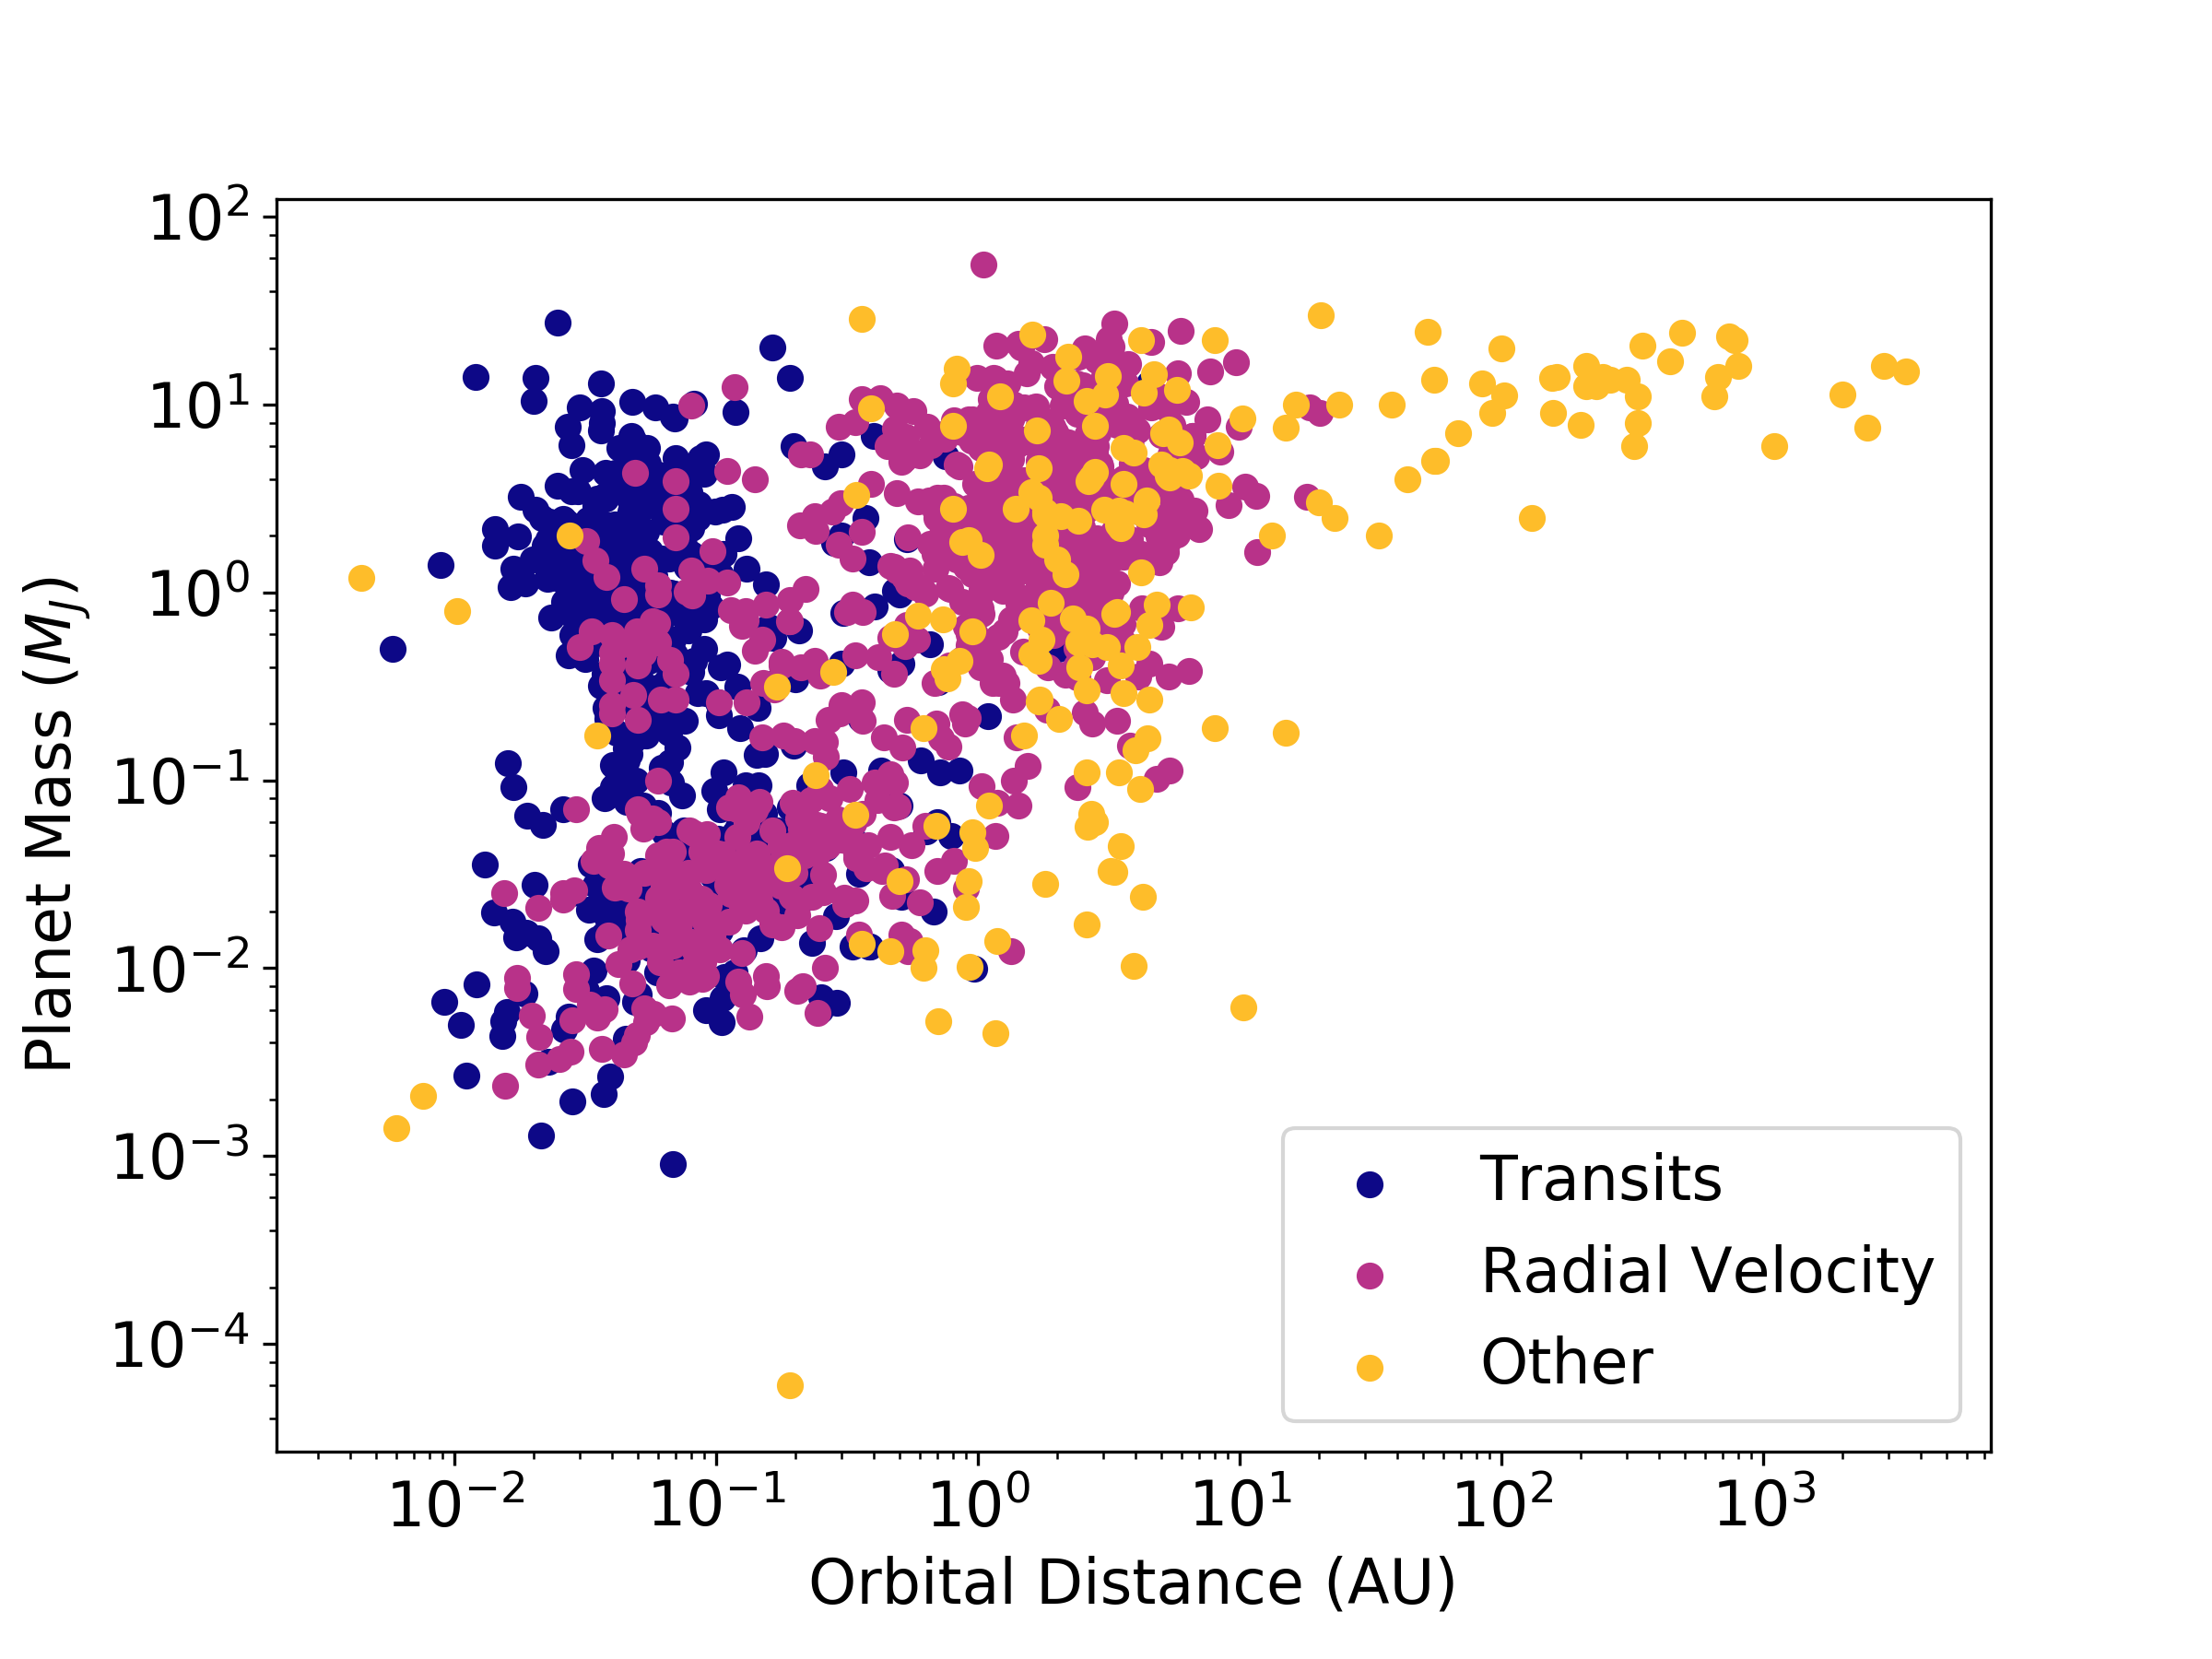
\includegraphics[width = \linewidth]{MA_NASAexo.png}
    \caption{Mass of the planet (or minimum mass for radial velocity planets) in Jupiter masses against the orbital distance in astronomical units for all of the confirmed exoplanets (4340 planets as of 5th February 2021, NASA Exoplanet Archive). Colors show the discovery methods: blue is transiting planets, purple is radial velocity detections and orange is all other detection methods. }
    \label{int:fig:MA}
\end{figure}

% Transit                          3306
% Radial Velocity                   823
% Microlensing                      106
% Imaging                            51
% Transit Timing Variations          21
% Eclipse Timing Variations          16
% Pulsar Timing                       7
% Orbital Brightness Modulation       6
% Pulsation Timing Variations         2
% Astrometry                          1
% Disk Kinematics                     1

On average, 50\% of the stars in our galaxy host at least one planet \citep{Howard2012,Dressing2013,Batalha2013,Silburt2015}. The 4,340 exoplanets confirmed to date range from small rocky planets to large gas giants. Figure  \ref{int:fig:MA} shows a plot of mass vs orbital distance of all these planets colour-coded by discovery technique. Out of the many methods employed, two account for the vast majority of discoveries: transiting planets (3306 planets, shown in blue) and radial velocity planets (823 planets, coded purple).

Transiting planets pass in front of their star and create a periodic shadow in the flux measured from their star. Radial velocity planets are detected by observing a signature of the movement of the host star due to the gravitational pull throughout the planetary orbit. Other techniques - represented by the colour orange in Figure \ref{int:fig:MA} - include microlensing, imaging, transit/eclipse timing variations, and pulsar timing.

The exoplanet population can be broadly classified into four families according to mass. At the lower end of the mass spectrum are the terrestrial planets, similar to the four smallest planets of our solar system: Mercury, Venus, Earth and Mars. Within this group fall  exoplanets with masses similar to the mass of Earth (around 0.5-2 $M_\oplus$ and sometimes even smaller). The second family are the Super-Earths. These planets are more massive than Earth (1 $M_\oplus = 3.1\times10^{-3} M_J$) but less massive than Uranus or Neptune and orbit their host stars at distances shorter than that between Earth and the Sun. Terrestrial planets and Super-Earths occupy the bottom left cluster of Figure \ref{int:fig:MA}. Super-Earths are considered the most abundant in our galaxy \citep{Borucki2011,Howard2012,Morton2014,Batalha2014,Petigura2013,Petigura2018,Fulton2017,Bryson2020}. Rocky planets on short period orbits close to their host stars are known as hot-rocks or lava planets. They are so hot that their surface is mostly or entirely covered by lava oceans \citep[e.g.,][]{Leger2011, Elkins-Tanton2012, Winn2018}.

The third family is the Neptunian exoplanets, with masses similar to those of Neptune and Uranus. These are planets with rocky cores and  hydrogen/helium-dominated atmospheres. Warm-Neptune (2-6$M_\oplus$ on short orbital periods) are a ubiquitous outcome of planet formation, occurring around more than 25\% of all stars \citep[e.g.,][]{Buchhave2014, Fulton2017}.

Finally, the largest exoplanets have masses similar to that of Jupiter. Due to their size, these planets are the easiest to find with current detection techniques. However, in absolute numbers, they are less common as other types of planets \citep[e.g.,][]{Gould2006,Howard2012,Fressin2013,Santerne2012,Wright2012}. Cooler Jupiter-like planets (top right cluster of Figure \ref{int:fig:MA}) are predominantly discovered by radial velocity and are ideal targets for direct imaging. In contrast,  "hot Jupiters" (top left cluster of Figure \ref{int:fig:MA}) are mostly discovered by the transit method. Hot Jupiters are, as the name suggests, a similar mass to Jupiter but are on orbits that lie within the orbit of Mercury and so receive much more insolation from their host stars. As a result, their temperature is typically more than 1500K (1200$^\circ$C).  It is these gas giant planets that are the focus of this thesis.

% Aside from these main groups, there are also rocky planets smaller than super-Earths, some are on extremely short orbits, and these are dubbed the "hot-rocks". There are also ice giants like Neptunes or sub-Neptunes and smaller gas giants like Saturn or sub-Saturn type planets.

\subsection{The strength of the multiple system planets: masses from TTVs}% ( a short section on TTVs)

Out of the 4,000+ exoplantes discovered to date, 1864 belong to 745 multi-planet systems. Gravitational interactions between planets in the same system cause the planets to deviate from Keplerian orbits. This means that the orbital period is no longer a constant value and thus the time between each transit (planet crossing the star) will vary. This phenomenon is called transit timing variation (TTV). TTVs are useful in many areas of exoplanet science \citep[e.g.,][]{Schneider2003, Agol2005, Holman2005}. For example, they have been used to infer the presence of a non-transiting planet in a system where at least one planet is transiting or to confirm that a transit signal is indeed due to a planet and not a false positive. Additionally, TTVs can be used for planet characterization by constraining the masses and other orbital elements \citep[e.g.,][]{Ballard2011, Holman2010, Carter2012}.

 The Kepler mission provided four years of almost continuous optical photometric observation of several hundred multi-planet systems. Several studies have used this data to constrain the parameters of the orbital dynamics and planetary masses. In Chapter \ref{TTVs} of this thesis, we follow up on four of these systems using multiple transit observations per planet. We aim to confirm the TTV signal at another wavelength (near infrared with Spitzer/IRAC compared to optical with Kepler), to lengthen the baseline of the previous Kepler observations and to look for signatures of more planets.

\section{Exoplanet atmospheres}
\subsection{Methods for probing exoplanet atmospheres}% (Look at Jacob’s 1.2)

There are two main methods for characterizing the atmospheres of exoplanets: direct imaging and transmission/emission spectroscopy, at either high or low resolution. The probability of a planet transiting is $R_s/a$, where $R_s$ is the stellar radius and $a$ is the planetary orbital distance \citep{Borucki1984}. This results in a very small fraction of the total planets to be viable for transmission spectroscopy. Direct imaging can be used to observe the atmospheres of non-transiting planets. However, directly imaging exoplanets is difficult since telescopes and observatories have to overcome the very high contrast ratios between the star and the planet. With the detectors quickly becoming saturated by the stellar flux there is often not enough time to gather enough photons from the planet. Nevertheless, with state-of-the-art coronagraphic and adaptive optics systems, several exoplanets have been directly imaged \citep[e.g.,][]{Marois2008,Marois2010,Lagrange2010,Rameau2013,Kuzuhara2013}.

This thesis focuses on characterizing the atmospheres of transiting planets.The transit method is a common technique for discovering planets. The measured transit depth and eclipse depth are wavelength and atmospheric composition-dependent quantities so can also be used to observe and study the atmospheres of planets \citep[e.g.,][]{Seager2000a, Brown2001, Charbonneau2005, Deming2005a}. In Figure \ref{int:fig:phasecurve} we show a schematic of a planet orbiting a star, which includes the transit (the planet in front of the star), the eclipse (the planet behind the star), and this full observation is called a phase curve. These techniques can each be used to study the properties of planetary atmospheres, giving us different parts of the story each time.

\begin{figure}
    \centering
    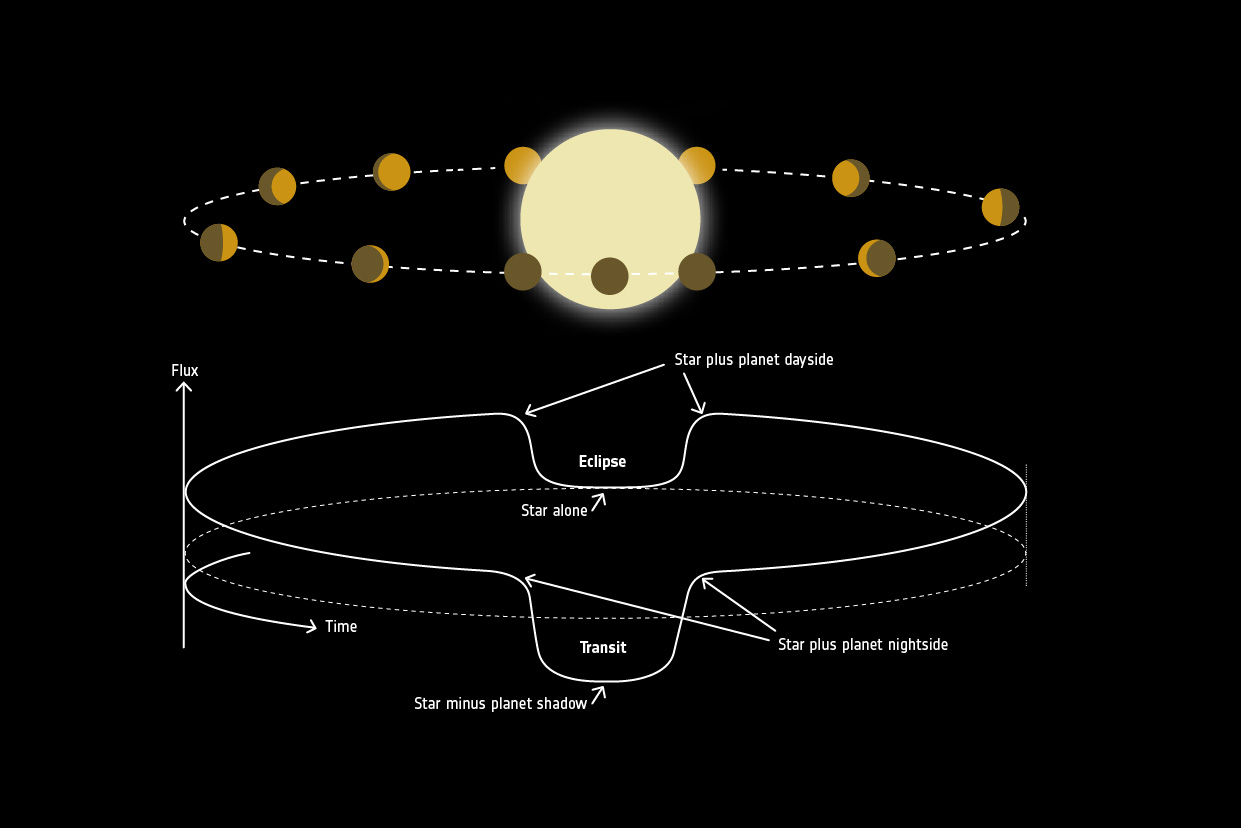
\includegraphics[width = \linewidth]{Exoplanet_phase_curve.jpg}
    \caption{Illustrative graphic detailing the full orbit of a planet around its host star, showing the transit and the eclipse. The full orbit observation is known as the phase curve, it captures all phases of the planet's tidally locked dayside. Image Credit: ESA}
    \label{int:fig:phasecurve}
\end{figure}

\subsubsection{Transmission spectroscopy}

The dimming of the stellar light when the planet passes in front of the star has a characteristic depth. This depth is a measure of the radius of the planet relative to the radius of the star (\rprss). However, during the transit, a small fraction of the starlight passes through and is partially absorbed by the upper atmosphere of the planet. This atmospheric absorption is wavelength dependent due to the opacities of different molecular and atomic species. At wavelengths where the atmosphere is more opaque, the transit depth will appear larger due to absorption of the stellar light, and where it is more transparent the transit depth will be smaller. Observing the planet transit across different wavelengths results in a transmission spectrum of the atmosphere. Models of the chemistry that causes the absorption features can be compared with observations to gain insights into the atmospheric composition \citep{Charbonneau2002, Vidal-Madjar2003, Tinetti2007, Swain2008}.

Typically, differences in the transit depth are larger for hot, puffy atmospheres with large scale heights ($H$), where:

\begin{equation}
    H = \frac{k_B T}{\mu_m g},
\end{equation}

and $T$ is the temperature, $\mu_m$ is the mean molecular mass, $g$ is the gravitational acceleration and $k_B$ is Boltzmann's constant. The scale height is a measure of the increase in altitude when the atmospheric pressure decreases by a factor of $e$, and for hot Jupiter atmospheres is on the order of a few hundred kilometers. In many cases, we use the equilibrium temperature ($T_{\rm eq}$) for $T$ and the planetary surface gravity for $g$. The measured difference in the transit depth (\rprss) resulting from an absorption feature can be written in terms of the number of scale heights crossed ($N_H$),

\begin{equation}
\Delta \delta = \frac{\pi(R_p + N_H H)^2}{\pi R_s^2} -
\frac{\pi R_p^2}{\pi R_s^2}
 \approx 2 N_H \delta \left(\frac{H}{R_p}\right).
\label{int:eq:NH}
\end{equation}

where $\delta$ is the transit depth (\rprss) and $\Delta\delta$ is the difference in the transit depth inside and outside a molecular feature. Hotter planets are expected to have a larger signal, due to the dependence on $H$ which scales with the temperature. However, the technique of transmission spectroscopy has successfully been applied to cooler targets as well \citep[e.g.,][]{Desert2011b, Berta2012, Crossfield2017}. In Chapter \ref{transits} we use equation \ref{int:eq:NH} to determine on average how many scale heights the Spitzer Space Telescope probes between 3.6 and 4.5~\um~for a survey of 49 transiting planets ranging from 600 to 2600 Kelvin. %The mean scale height for this sample of planets is 550$\pm$330~km.
In Chapter \ref{transits} we show that, for our sample of planets, we probe an average of 0.5 scale heights between the two Spitzer/IRAC bandpasses at the 7$\sigma$ level.

\subsubsection{Emission Spectroscopy}

The dayside emission of a planet can be measured by observing the planet before, during, and after it passes behind the star. Similar to the transit, this creates a dip in the light measured throughout time. The depth of that dip, or the eclipse depth, is a measure of the fractional flux of the planet relative to the star (\fpfs). Here, $F_p$ and $F_s$ are used to represent the disk-averaged spectral density multiplied by the disk area for the planet and the star respectively. The eclipse depth, in absence of any spectral features, can be represented by the ratio of two Planck functions multiplied by the transit depth,

\begin{equation}
\frac{F_p(\lambda)}{F_s(\lambda)} = \frac{B_\lambda(T_p)}{B_\lambda(T_s)}~\frac{R_p^2}{R_s^2},
\end{equation}

where $B_\lambda(T)$ is the Planck function,

\begin{equation}
B_\lambda(T) \equiv \frac{2hc^2}{\lambda^5} \frac{1}{e^{hc/(\lambda k_B T)} - 1}
\end{equation}

in which $T$ is the temperature of the planet or the star, $\lambda$ is the wavelength, $h$ is Planck's constant, and $c$ is the speed of light. Assuming the temperature of the star is known, this formulation can also be used to solve for the planetary temperature at a specific wavelength, this is known as the brightness temperature, $T_B$. In Chapter \ref{eclipses}, we use this formula and rigorously integrate it over the stellar models instead of a blackbody for the star. Next we incorporate the Spitzer spectral response functions to accurately calculate the brightness temperatures of a survey of planets with emission at 3.6 and 4.5~\um~.

Unlike transmission spectroscopy, where the starlight is passing through the stellar atmosphere, emission spectroscopy measures the emission of the planet relative to the star. The emission spectrum of the planet will deviate from a blackbody depending on the atmospheric composition and temperature structure probed by the photons traveling through the atmosphere (see Section \ref{} for more on the temperature structure). The crucial difference between the information gathered from transmission spectroscopy and emission spectroscopy is the depth probed in the atmosphere. Due to the slant geometry, an optical depth of 1 is reached at much lower pressures in transmission compared to the normal geometry in emission \citep{Fortney2005}. In general, transmission spectroscopy probes the upper more tenuous layers of the atmosphere at pressures around 1 millibar, whereas emission spectroscopy probes deeper layers at pressures of around 0.1-10 bar (depending on the wavelength).

\subsubsection{Phase curves}

A phase curve observation consists of observing the planet throughout its entire orbit, including the transit and the eclipse. Planets on close-in orbits of $\lesssim10$ days typically become tidally locked, with permanent day and night sides \citep[e.g.,][]{Guillot1996}. Therefore, a phase curve allows us to observe the planet as a function of its rotational phase, as demonstrated in Figure \ref{int:fig:phasecurve}. At each orbital phase, different longitudes of the planet's dayside are rotating into the view of the observer. The difference in brightness between any two points in phase can be used to reconstruct a brightness map of the planet's surface \citep{Knutson2007, Knutson2012, Crossfield2012, Borucki2009, Snellen2009}. At optical wavelengths, the planetary brightness is dominated by reflected light from the star, and so a phase curve observation provides constraints on the planet's albedo. On the other hand, at infrared wavelengths, the planetary brightness is dominated by thermal emission, resulting in longitudinal information about the planet temperature \citep{Parmentier2018b}.

On top of the eclipse depth (\fpfs) and the transit depth (\rprss), a phase curve observation can provide us with the measurement of the maximum flux, the phase of the maximum flux relative to eclipse (known as the phase curve offset), and the relative amplitude of the phase curve (day-to-night temperature contrast). Since these planets are tidally locked, the substellar point is brighter than the limbs of the planet. This brightest point can lag (negative offset, westward shift) or lead the substellar point (positive offset, eastward shift). These shifts are measured with the phase curve offset as well as the day-to-night temperature contrast \citep{Showman2002}. Parameterising the phase curve like this is useful for studying the energy balance and the dynamics of the atmosphere \citep{Cowan2012b, Schwartz2015}. In Chapter \ref{eclipses}, we use the phase curve offset measured in each of the two Spitzer/IRAC bandpasses to determine if a measurement of the efficiency of redistribution from eclipses will change over the two wavelengths.

Similar to transits and eclipses, these phase curves can be measured spectro-photometrically or spectroscopically. At the wavelengths with a strong opacity source and strong atmospheric absorption, a phase curve probes higher in the atmosphere (at low pressures), whereas outside an absorption band the phase curve observation probes deeper (high pressures) \citep{Showman2009, Kataria2015}. This technique allows for maps of the chemistry and temperature structure and a map of the flux and brightness temperature \citep{Cowan2008, Showman2008, Knutson2009c, Stevenson2017}. Furthermore, \citet{Arcangeli2021} measured the first emission spectrum at quadrature without the need to observe a full phase curve observation of WASP-12b.

\subsection{Instrumentation for probing exoplanet atmospheres used in this thesis} %(your previous 2.2)

This thesis mainly focuses on using multi-epoch observations of exoplanet atmospheres in emission and transmission in the two photometric bandpasses of the Spitzer Space Telescopes Infrared Array Camera (Spitzer/IRAC) \citep{Werner2004}. In Chapter \ref{eclipses} we expand on our work with Spitzer by studying full emission spectra taken with the Hubble Space Telescope Wide Field Camera 3 (HST/WFC3) to compare the effects of atmospheric properties at different wavelengths and depths in the atmosphere. Both of these telescopes are space-based observatories, which are advantageous over ground-based observatories as they offer both stability and sensitivity while bypassing the Earth's atmosphere. This is especially  important for this work because the atmosphere of the Earth absorbs in the infrared where there are absorption signatures of the particular  molecules that we study, such as water vapor and carbon dioxide.

\subsubsection{Spitzer/IRAC}

Launched in 2003, Spitzer Space Telescope was cryogenically cooled with liquid helium cryostat to 15K and could observe between 3 and 24~\um~ over four photometric bands with the Infrared Array Camera \citep[IRAC,][]{Fazio2004}. In 2009, Spitzer exhausted its supply of liquid helium and entered the post-cryogenic mission, so called ``Warm-Spitzer'' at $\sim$30K \citep{Mcmurtry2006}, with just the two shorter wavelength bands remaining active, 3.6 and 4.5~\um. After 16 years of observations, the Spitzer Space Telescope was decommissioned on the 30th of January 2020. Nevertheless, there remains a wealth of knowledge available from the archival data, which is a focus of this thesis. The two remaining wavelength bands of Spitzer/IRAC mainly capture the atmospheric signatures of methane (\ce{CH4}), carbon monoxide (\ce{CO}), carbon dioxide (\ce{CO2}), and water (\ce{H2O}). In Chapters \ref{transits} and \ref{eclipses} we show the atmospheric opacities of the molecules probed with Spitzer/IRAC in emission and transmission respectively.

\subsubsection{HST/WFC3}

The Hubble Space Telescope contains some of the current best instruments for measuring the atmospheres of exoplanets. The Wide Field Camera 3 (WFC3) is capable of measuring spectra from 0.8 to 1.7~\um~ with two separate grisms. In Chapter \ref{eclipses} we use the emission spectra measured with the WFC3/G141 grism, which captures the 1.4~\um~ water feature, and combine these observations with our Spitzer/IRAC photometry.

\subsection{Systematics and Noise Sources}

When attempting to measure the precise signal of an exoplanet atmosphere, dealing with the various noise sources becomes very important. The first noise source is unavoidable, photon noise or shot noise. Each atom inside the star emits a photon with some probability, this probability follows a Poisson distribution with a standard deviation of $\sqrt{N}$, where $N$ is the number of events or counts detected. The other noise sources to correct for are the background noise, dark current, and readout noise. Background noise is the incoming light on the detector in the absence of any apparent sources (e.g. zodiacal light). Dark current arises from thermal fluctuations in the electrons of the detector. Readout noise is the amount of noise generated from the electronics itself which is a similar contribution to the background noise for Spitzer. In our analysis, we measured and subtracted the background from our observations using several different techniques and determined which was the best for each planet.

\subsubsection{Spitzer/IRAC intrapixel sensitivity}

\begin{figure}
    \centering
    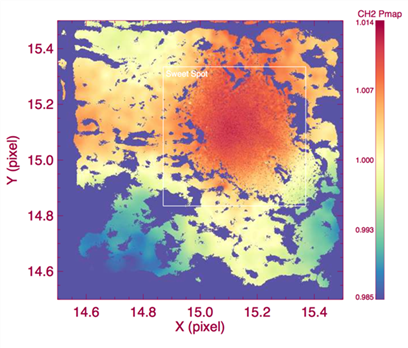
\includegraphics[width = \linewidth]{IRAC_Instrument_Handbook183.png}
    \caption{Map of the intrapixel sensitivity of the central pixel on the detector at 4.5~\um~ for warm-Spitzer/IRAC data. The x and y axis show the fraction of the central pixel and the colour map shows the pixel sensitivity with red showing a higher sensitivity. Image Credit: Spitzer/IRAC Instrument Handbook\footnote{https://irsa.ipac.caltech.edu/data/SPITZER/docs/irac/iracinstrumenthandbook/47/}.  }
    \label{int:fig:pmap}
\end{figure}

Each instrument has challenges regarding detecting the signals of exoplanet atmospheres since none of the facilities used were designed with exoplanet characterization in mind. The most important and strongest instrumental effect that we need to account for with Spitzer data is the gain variations within a single pixel, known as the intrapixel sensitivity effect. Figure \ref{int:fig:pmap} demonstrates the photometric gain at 4.5~\um~of the central pixel of the Spitzer/IRAC detector. The target moves across the detector due to the following effects: a settling drift after slewing, a long-term drift due to an inconsistency in velocity corrections, jitter, and a thermally induced oscillating pointing drift due to periodic on-off cycling of the battery heater within the spacecraft. This movement in combination with the changes in gain causes temporal variations in the amount of flux measured from a constant source. The typical signature of a few scale heights in the atmosphere of a hot Jupiter is about 100 parts per million (0.1\%). The amplitude of the intrapixel variations seen in Spitzer lightcurves is on the order of 1\%. Thus, we need to accurately correct these systematics to obtain the precision required to detect atmospheric signatures.

We typically overcome the settling drift by having a peak-up throw-away observation of about half an hour and by discarding ~15 minutes from the beginning of the observation. Next, we model the long-term settling drift with a linear function of time. There have been many efforts over the years to model and correct the periodic systematics induced from the pointing variations \citep[e.g.,][]{Charbonneau2008,Ballard2010, Knutson2012,Stevenson2012, Evans2015, Morello2015a, Morello2015b, Buzasi2015, Deming2015, Krick2016}.

% \begin{itemize}
% \item Polynomial fitting \citep{Charbonneau2008}
% %\item MCMC Evaluation \citep{Gillon2010}
% \item Kernel Regression Mapping, using the data to be corrected \citep[KR/Data;][]{Ballard2010, Knutson2012}
% \item BiLinearly Interpolated Subpixel Sensitivity \citep[BLISS;][]{Stevenson2012}
% \item Gaussian Process Models \citep[GP;][]{Evans2015}
% \item Independent Component Analysis \citep[ICA;][]{Morello2015a, Morello2015b}
% \item Segmented Polynomial for the K2 Pipeline \citep[SP(K2);][]{Buzasi2015}
% \item Pixel Level Decorrelation \citep[PLD;][]{Deming2015}
% \item Kernel Regression using a calibration pixel mapping dataset \citep[KR/Pmap;][]{Krick2016}
% \end{itemize}
All of these different methods culminated with a repeatability and reliability data challenge, the results of which were presented in \citet{Ingalls2016}. Each of the methods were tested on 10 real and 10 simulated eclipses of XO-3b. The data challenge found that most of the methods were able to estimate accurate uncertainties on individual eclipses. However, they found that BiLinearly Interpolated Subpixel Sensitivity \citep[BLISS;][]{Stevenson2012}, Pixel Level Decorrelation \citep[PLD;][]{Deming2015}, and Independent Component Analysis \citep[ICA;][]{Morello2015a, Morello2015b} were the most accurate and repeatable for correcting systematics on observations of large pointing fluctuations. Furthermore, they found that PLD was also able to obtain the highest accuracy on a similar simulated dataset. In this thesis, we focus on using PLD \citep{Deming2015}, while also testing the original polynomial fitting \citep{Charbonneau2008} as well as Gaussian Process models \citep[GP;][]{Evans2015}.

\subsubsection{Pixel Level Decorrelation}

Unlike several of the other techniques, Pixel Level Decorrelation \citep{Deming2015} does not require knowledge of the sub-pixel position or a map of the variations in the sub-pixel sensitivity. Instead, it assumes that the flux from the star will be a smooth function of position, such that when the target moves on the detector, the neighboring pixels will receive more flux when the target moves towards them and less flux when the target is moving away from them. The sub-pixel position is therefore encoded implicitly in a generalized function of pixel intensity. Such a smooth function can be differentiated and therefore can also be Taylor expanded. Doing this allows us to model the flux in time as a weighted sum of individual pixel fluxes. To model the full photometric lightcurve in time ($t$) we combine the weighted pixel flux sum with a transit/eclipse model ($DT(t)$) and a linear slope in time ($ft$) to model the long-term drift:

\begin{equation}
    \Delta S^t = \sum_{i=1}^{N}c_i \hat{P}_i^t + DT(t) + ft,
\end{equation}

where $S^t$ is the flux measured over time and $\Delta$ represents the total fluctuations from all sources. $\hat{P}_i^t = \frac{P_i^t}{\Sigma_{i=1}^{N}P_i^t}$ represents the normalized flux from pixel $i$ at time $t$, where a grid of $i$ pixels are chosen around the centroiding position.

\subsection{Properties and Climates of exoplanets}%  (look at Arcangeli section 1.3)

\subsubsection{Chemistry}

Since hot Jupiters are gas giants, their atmospheres are primarily composed of gaseous Hydrogen and Helium \citep{Seager1999}, with most of their other constituents also being in gas phase, such as water, methane, and carbon monoxide \citep{Brown2001}.

A typical assumption when modeling atmospheres is that the chemical composition of the atmosphere is  the same as our Sun (solar composition): 74.9\% Hydrogen and 23.8\% Helium, with all the heavier elements (which are known as \textit{metals} in astrophysics) encompassing the other 1.3\%. Starting from this assumption, a series of chemical networks are used to calculate the abundances of molecular species in the atmosphere. A common assumption for these chemical networks is that the atmosphere is in chemical equilibrium, meaning that the molecular abundances can be determined, in the first order, from the temperature and pressure alone. Under these assumptions, predictions can be made about which molecules would be expected to be abundant for different temperatures of planets.

Spitzer is an invaluable tool to test this assumption because it is sensitive to the abundance of methane, water, carbon monoxide and carbon dioxide (\ce{CH4} and \ce{H2O} at 3.6~\um~ and \ce{CO}, \ce{CO2}, \ce{H2O}) at 4.5~\um~). The strength of the \ce{H2O} opacity is approximately equal in both Spitzer/IRAC bandpasses (see Figure 1 of Chapter \ref{eclipses}), therefore Spitzer can be used to probe the relative abundance of CO and \ce{CH4} \citep{Madhusudhan2019}. Since these are both carbon-bearing species, and since carbon (C) is less abundant than hydrogen (H) and oxygen (O), there is a trade-off between CO and \ce{CH4} with temperature. The following summary chemical reaction arising from the \ce{CH4}-CO conversion reaction scheme plays an important role in determining the dominating carbon-bearing species in an atmosphere \citep[e.g.,][]{Visscher2010, Moses2011, Visscher2011}:
\\
\ce{ \centering CH4 + H2O <=> CO + 3H2}.
\\
For a nominal pressure of 1 bar, temperatures higher than $\sim1100$~K favor \ce{CO} creation, and lower temperatures favor \ce{CH4} creation \citep[e.g.][]{Madhusudhan2012, Molliere2015, Molaverdikhani2019}. Therefore, hotter planet atmospheres are predicted to have carbon monoxide and cooler planets are predicted to have methane as the dominant carbon-bearing species, with the transition occurring at around 1100K, depending on the pressure being probed (emission probes deeper than transmission).

In reality, there are several phenomena that can cause an atmosphere to deviate from equilibrium: photochemistry, vertical mixing, higher metallicity, cloud/haze formation, tidal heating, winds, and other dynamical interactions \citep[e.g.,][]{Madhusudhan2019}. In Chapter \ref{transits} we study the effects of some of these processes by modeling them and comparing several different grids of models to a survey of 50 planets in transmission.

%Should I mention Vertical Mixing here? Photochemistry.

\subsubsection{Temperature structure}

% \begin{figure}
%     \centering
%     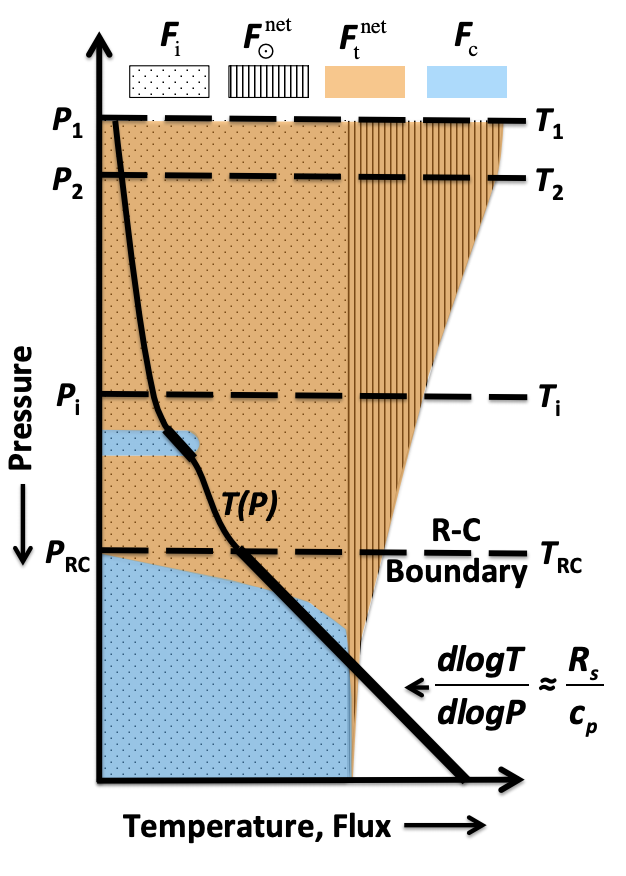
\includegraphics{modelTP.png}
%     \caption{Schematic figure of the temperature structure of a nominal (non-inverted) atmosphere, temperature increases with increasing pressure. $F_{\rm i}$ shows the internal heat flux,  $F_{\rm t}^{\rm net}$ shows the net thermal flux, and $F_{\rm c}$ shows the convective flux and $F_\odot^{\rm net}$ shows the absorbed stellar flux (if irradiated). The net thermal flux, convected flux and irradiated flux (if non-zero) must sum to the internal heat flux i.e. $F_{\rm i}$ = $F_{\rm t}^{\rm net}$ + $F_{\rm c}$ + $F_\odot^{\rm net}$. Image credit \citet{Marley2015}.}
%     \label{fig:my_label}
% \end{figure}

\begin{sidewaysfigure}
    \centering
    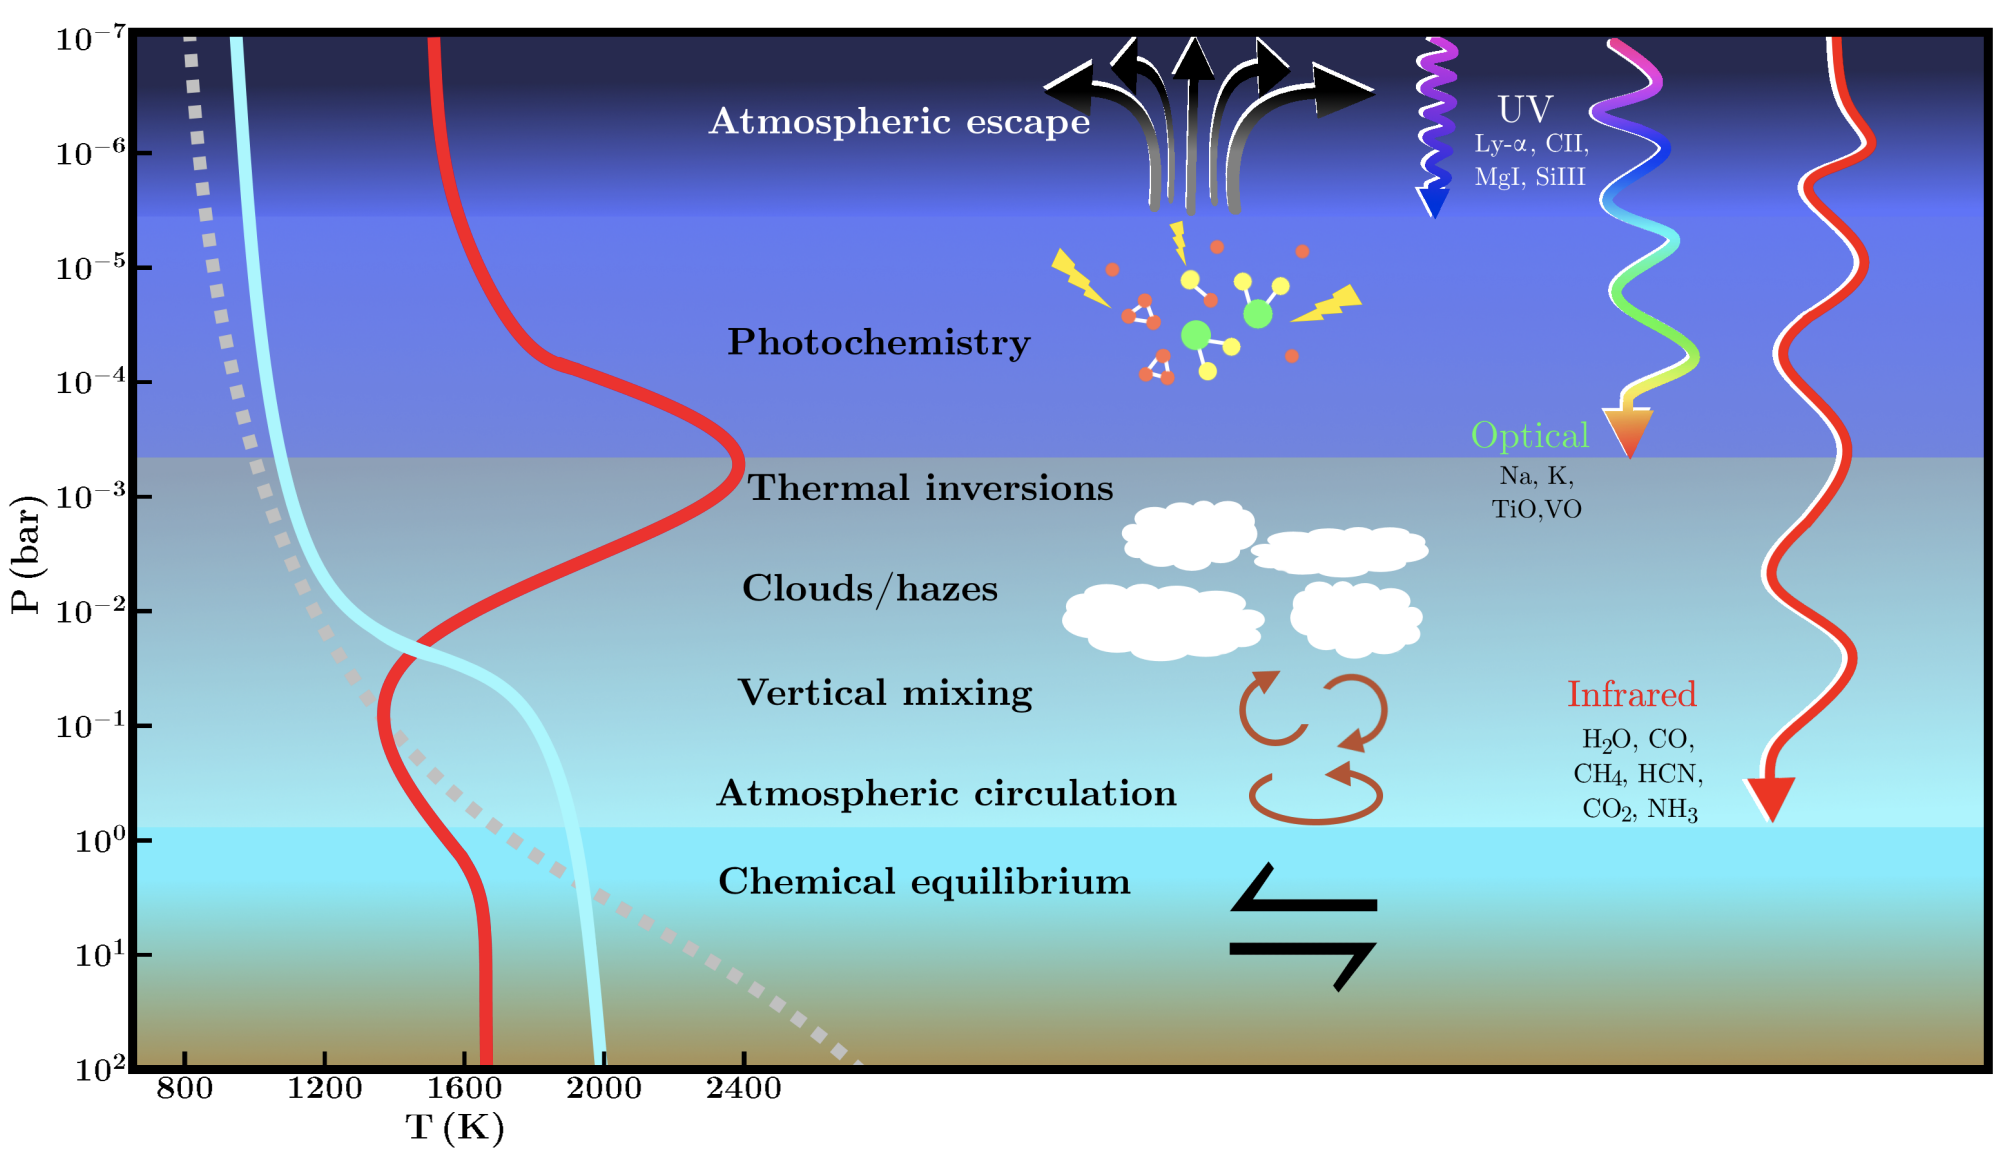
\includegraphics[width = \linewidth]{TPandeffects.png}
    \caption{Properties and processes active in the atmospheres of exoplanets. On the left and 3 model temperature-pressure profiles: grey-dashed is that of a non-irradiated atmospheres, cyan is an irradiated atmospheres with a nominal temperature-pressure profile and red is a highly irradiated atmosphere with a temperature inversion. Image Credit: \citep{Madhusudhan2019}}
    \label{int:fig:TPs}
\end{sidewaysfigure}

Just like on Earth, the temperature of a hot Jupiter atmosphere does not remain constant with altitude, i.e., it is not isothermal. Typically, the atmosphere gets hotter towards higher pressures. The gray dashed line in Figure \ref{int:fig:TPs} shows a typical temperature-pressure profile of a model atmosphere. In the deep atmosphere, at high pressures, the atmosphere is opaque and the energy is therefore transported convectively via bulk movement of gas. This results in inefficient transport and a large temperature gradient. Whereas in the upper more tenuous atmosphere, energy is transported radiatively which is a more efficient process, resulting in less steep temperature gradients.

The cyan line in Figure \ref{int:fig:TPs} shows an irradiated atmosphere with a nominal (non-inverted) temperature-pressure profile. The red line shows that of a highly irradiated atmosphere with a temperature inversion. A temperature inversion is where the temperature starts to increase with decreasing pressure. This is caused by the UV/visible absorption of the strong incident stellar irradiation, leading to the heating of the upper layers of the atmosphere. Earth's stratosphere contains a thermal inversion due to the absorption of Ozone (\ce{O3}). In hot Jupiters, molecules such as titanium oxide (\ce{TiO}) and vanadium oxide (\ce{VO}) are thought to be the cause of their thermal inversions \citep{Hubeny2003, Fortney2008, Desert2008}. However, recent work has also suggested that temperature inversions in ultra-hot Jupiters may be caused by the absorption of metals and metal hydrides \citep[Fe, Mg, SiO][]{Lothringer2018} or other metal-rich species \citep[AlO, CaO, NaH and MgH][]{Gandhi2019}.

The detection of molecular features in exoplanet atmospheres via emission spectroscopy not only tells us about the atmospheric chemistry on the dayside but it is also a probe of these vertical temperature profiles. For a nominal temperature-pressure (TP) profile (temperature decreasing with altitude), if a molecule is present and has an opacity at the wavelength of observation, then it will absorb the radiation and the measured eclipse depth will be smaller than the continuum. For example, Figure \ref{int:fig:w43} shows an HST/WFC3 spectroscopic observation from \citet{Stevenson2014c} where the 1.4~\um~ water absorption feature can be seen clearly in the emission spectrum. The temperature-pressure profile retrieved for the dayside of WASP-43b is very similar in shape to the diagram of an irradiated atmosphere in Figure \ref{int:fig:TPs}.

For an inverted TP profile, a molecule will emit radiation at a temperature higher than the continuum and so the eclipse depth will appear larger at the wavelength of the opacity. Figure \ref{int:fig:w18} shows an emission spectrum of WASP-18b, where you can see the 4.5~\um~ CO feature appearing in emission due to the temperature inversion. There have been a few studies finding evidence for temperature inversions in hot and ultra-hot Jupiters \citep[e.g.,][]{Knutson2008,Knutson2009b,Madhusudhan2010,Haynes2015,Evans2017,Arcangeli2018}. However, some of the early observations were revised \citep[e.g.,][]{Diamond-Lowe2014} as temperature inversions were notoriously difficult to establish in the available observations of hot Jupiters. In Chapter \ref{eclipses} we use our sample of planets in emission with Spitzer/IRAC observations to statistically measure a transition from the hot Jupiters to the ultra-hot Jupiters which is likely due to temperature inversions,among other effects.

\begin{sidewaysfigure}
    \centering
    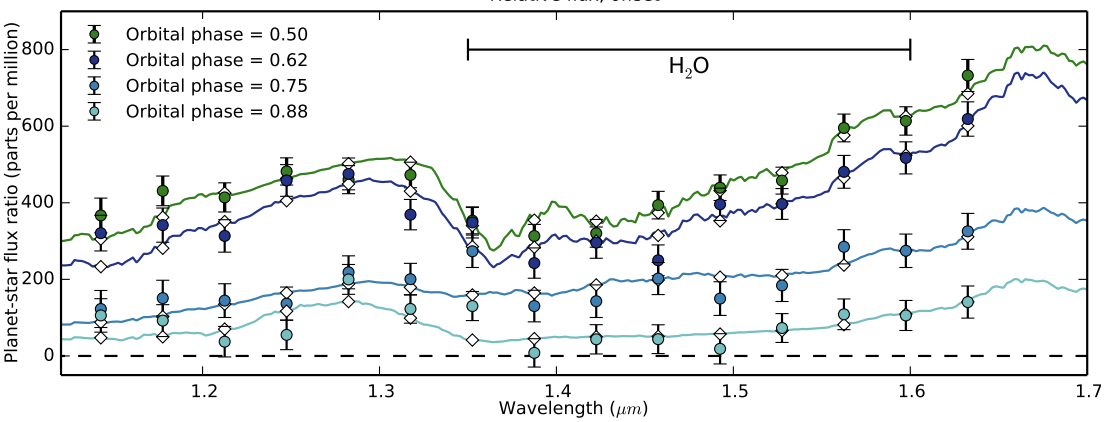
\includegraphics[width = \linewidth]{Wasp-43b_water.png}
    \caption{Emission spectrum of WASP-43b taken from a spectroscopic phase curve observation. Green data and model shows the emission spectrum during phase 0.5, which is what would be observed with an eclipse only observation. This clearly shows the water absorption feature appearing due to a nominal temperature-pressure profile. Other lines show the planet as it approaches quadrature (phase 0.75). At quadrature, you are observing half of the dayside and half of the nightside. Image credit: \citet{Stevenson2014c}.}
    \label{int:fig:w43}
\end{sidewaysfigure}

\begin{sidewaysfigure}
    \centering
    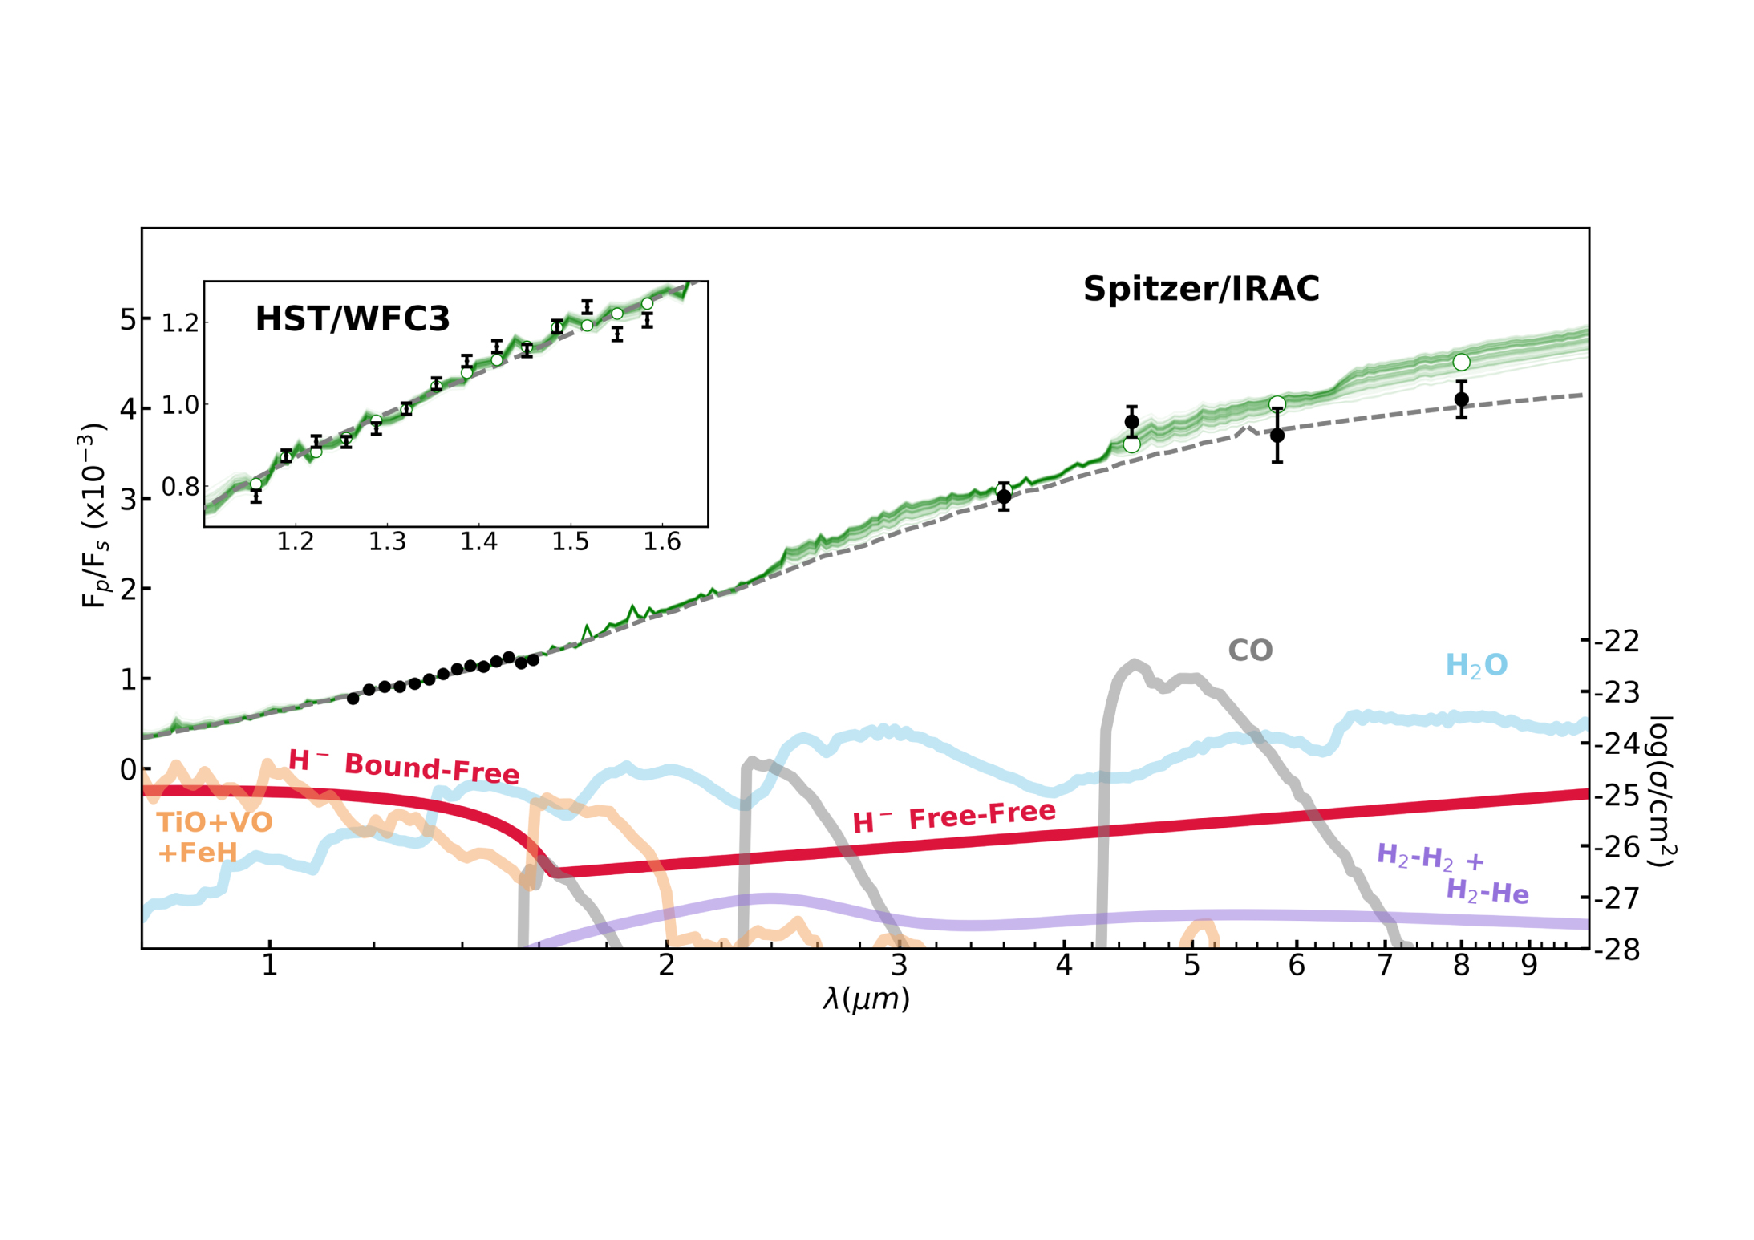
\includegraphics[width = \linewidth]{arcangeli+18.pdf}
    \caption{Emission spectrum of WASP-18b from HST and Spizter/IRAC (black data points). Green lines show the retrieved models, and the cross-sections of the important opacity sources are shown on the bottom of the Figure. The 4.5~\um~ Spitzer eclipse depth shows the CO feature appearing in emission due to the temperature-pressure profile. At the HST/WFC3 wavelengths, we see that the combination of \ce{H2O} and H- bound free opacity makes the emission appear like a blackbody. Image credit: \citet{Arcangeli2018}. }
    \label{int:fig:w18}
\end{sidewaysfigure}

Figure \ref{int:fig:TPs} also shows the pressure levels where several physical processes occur in planetary atmospheres. Each of these processes is also inexorably intertwined with the temperature-pressure structure, and we will discuss some of them individually in the following sections.

\subsubsection{Clouds and hazes}

In this thesis, I study gas giant exoplanets ranging from those cooler than the Earth \citep[Kepler-16b, 200K;][]{Doyle2011} all the way to the hottest ultra-hot Jupiter \citep[KELT-9b, 4000K;][]{Gaudi2017}. It is expected that, somewhere in the range of temperatures, aerosols will form. Aerosol is the all-encompassing term for clouds, hazes, and dust. Clouds are particles forming in the atmospheres as a result of first order phase changes. Due to the temperature-pressure profile crossing a condensation curve of some molecule, e.g. gas to liquid water. Cloud formation can also occur as a result of thermochemical reactions. On the other hand, haze formation can be defined as the formation of particles via the breakdown of molecules due to energy input e.g., photochemistry of energetic particle bombardment. Both clouds and hazes have the effect of dampening the atomic and molecular signatures seen in the atmospheres of exoplanets, sometimes making the transmission spectra appear mostly flat in the visible and near-infrared \citep[e.g.,][]{Charbonneau2002, Fortney2003, Pont2008}.

Even in our own solar system, aerosol composition is extremely diverse, from water on Earth, sulfuric acid on Venus \citep{Hansen1974}, ammonia on Jupiter and Saturn \citep{Booke1998, Baines2009} and many different complex organics and hydrocarbons on the outer solar system planets and moons \citep[e.g.,][]{Sromovsky2011, Romani1988, Sagan1992, Brown2002, Rages1992}. Aerosols were therefore predicted to be found in the atmospheres of exoplanets. In fact, the very first transmission spectrum of an exoplanet showed dampening of the predicted absorption feature by atomic sodium in the atmosphere of HD 209458b. One of the possibilities that could account for the reduced sodium abundance was the presence of high altitude aerosols \citep{Charbonneau2002}. Given equilibrium chemistry, different molecules/elements will condense to form clouds at different pressures \citep{Lodders2004}. This depends on when the temperature-pressure profile of the atmosphere crosses the condensation curves of the cloud forming species. Different molecules will be abundant in the atmospheres of planets of different temperatures, so different cloud layers are expected to form in planets of certain temperatures \citep{Marley2013}.

% transmission spectra
% emission spectra
% reflected light

As well as dampening molecular features in transmission spectra, clouds can leave their own spectral fingerprint. In particular, high altitude H2 particles create a Rayleigh scattering slope in the transmission spectra
%. Rayleigh scattering is the elastic scattering of light by particles, the intensity of light scattered by a particle goes as 1/$\lambda^4$ meaning that smaller wavelengths (bluer light) scatter more than longer wavelengths (redder light). This causes the transit depth to be deeper towards the blue part of the electromagnetic spectrum, creating the typical Rayleigh slope seen by observers
\citep[e.g.,][]{LecavelierdesEtangs2008,Sing2015, Sing2016, Gibson2017}. Similarly, clouds can plague our observations and leave spectral signatures via Mie scattering \citep[e.g.,][]{Benneke2019} or their own absorption features \citep[e.g.,][]{Wakeford2015}. It is hoped that in the future, the James Webb Space Telescope will be used to pin down the composition of aerosols using computations of possible cloud species \citep[e.g.,][]{Gao2020}.

\subsubsection{Dynamics and climate}

Atmospheric dynamics and climate are important factors that we need to consider when studying the spectral features or temporal appearance of exoplanet atmospheres. In Chapter \ref{transits}, we study the transmission spectra in the infrared at pressures where \ce{H2O}, \ce{CH4}, \ce{CO}, and \ce{CO2} are dominant. Dynamical mixing in the atmosphere can affect the local abundances of these observed species. Additionally, in Chapter \ref{eclipses}, we study the dayside brightness temperatures which can also be affected by large-scale atmospheric weather. Finally, in Chapter \ref{w18b} we measure variability in the dayside of an ultra-hot exoplanet atmosphere. This is a direct observation of time-variable atmospheric dynamics.

Based on timescale and gravitational arguments, hot Jupiters are expected to be tidally locked \citep[e.g.,][]{Rasio1996, Guillot1996}. This means that they always have one hemisphere facing the star, a permanent dayside, and one hemisphere facing away from the star, a permanent nightside. These will rotate into and out of view of an observer throughout a full phase curve observation. Phase curves provide a unique opportunity to study the structure of a planet at different longitudes and thus to understand more about their atmospheric dynamics. However, certain aspects of atmospheric dynamics can also be probed with eclipse-only and transit-only observations.

The permanent dayside of a planet receives all of the insolation from the host star, producing a strong horizontal temperature gradient that drives zonal and meridional winds. These winds redistribute heat from the dayside to the nightside of the planet. If the redistribution is very efficient then the temperature difference between the dayside and the nightside will be small, like on Venus. On hot Jupiters, the radiative and advective timescales are a similar order of magnitude, resulting in low efficiency of redistribution and allowing for strong day-night temperature contrasts to remain \citep[e.g.,][]{Showman2002, Perna2012}. The rate at which planets redistribute heat from the dayside to the nightside in their atmospheres is characterized by a so-called heat redistribution factor, $f$, which lies between 2/3 for a planet with no atmosphere and no heat redistribution and 1/4 for a planet that is extremely efficient at redistributing heat \citep[e.g.,][]{Koll2019}. The exact mechanisms involved in determining the value of this redistribution factor are unknown, and it is not parameterised by the physical properties of the atmosphere. However, there has been observational and theoretical evidence that hotter planets should be less efficient at redistributing heat to their nightsides \citep{PerezBecker2013, Schwartz2015}. In Chapter \ref{eclipses} we will revisit these pieces of evidence and propose that ultra-hot Jupiters display a broad range of redistribution efficiencies.

The strong longitudinal winds resulting from this temperature contrast can distort the temperature pattern, shifting the hottest point of the atmosphere eastward \citep[e.g.,][]{Showman2002}. These eastward hot-spot offsets have been observed and have been attributed to equatorial jets \citep[e.g.,][]{Knutson2012, Cowan2012a}. However, there has also been a detection of a westward hot-spot offset in CoRoT-2b \citep{Dang2018} and a variable hot-spot offset in HAT-P-7b \citep{Armstrong2016}. This could be explained by non-synchronous rotation, in the case of CoRoT-2b, or magnetic effects, in the cases of CoRoT-2b and HAT-P-7b. In addition to the day-night temperature contrast, it is possible that condensates can be transported from equatorial to polar regions through means of meridional circulation, which is suggested to be common in sub-Neptunes, hot Jupiters and ultra-hot Jupiters \citep{Parmentier2013, Ehrenreich2020}.

% Vertical mixing
As well as meridional winds and longitudinal winds there is also a vertical component to the dynamics in an atmosphere. The process of vertical (radial) transport prevents the gravitational settling of condensates as well as mixing chemical species from deeper in the atmosphere to observable pressures. This has the effect of changing the observed abundances away from those expected from equilibrium chemistry calculations. In the 1D chemical diffusion framework, vertical mixing is often modeled with an eddy diffusion co-efficient, $K_{zz}$ \citep[e.g.][]{Zhang2018b, Miles2020}. To capture all of these effects, 3D global circulation models are needed.

\subsubsection{Atmospheric variability}
\label{int:sec:variability}

In Chapter \ref{w18b} of this thesis, we measure variability in the brightness of an ultra-hot Jupiter, WASP-18b. Brightness variability is directly related to the dynamics and climate of atmospheres. Variability seems to be a common occurrence in brown dwarfs, with more than 50\% of L and T brown dwarfs displaying temporal variability of a few percent \citep{Metchev2015}. Variability has also been detected in directly imaged free-floating planets \citep{Biller2015} and even in Jupiter, which has been shown to be temporally variable in the equatorial banded structures observed at 5~\um~ \citep{Antunano2019}. The question is whether exoplanets would display some kind of temporal variability as well. Observing variability in an exoplanet requires long observations with high sensitivity and stability. Fortunately, we have 10 observed almost consecutive eclipses of WASP-18b with Spitzer/IRAC at 4.5~\um~, which allows us to study how the emission of the planet changes with time.

Ultra-hot atmospheres like WASP-18b can be significantly ionized, which can couple with the magnetic field of the planet and settle into an oscillatory pattern, creating variability in the brightness and the hot-spot offset \citet{Rogers2017}. Variable wind speeds, causing the advance and retreat of thermal structures, could lead to variable cloud coverage causing the emission from the dayside to vary \citep{Armstrong2016}. Furthermore, clouds can blow onto the dayside where they can then be photochemically destroyed and would generate brightness variability \citep{Jackson2019}.
%The brightness and temperature peak is predicted to be offset eastwards of the substellar point, however, the reflected light peak appears to be offset westwards to the substellar point \citep{Webber2015, Munoz2015}.

\subsubsection{Inflated hot Jupiters}

Due to the intense stellar insolation that a hot Jupiter receives compared to Jupiter, it is expected that their atmospheres and interior structure behave differently. \citet{Guillot1996} predicted that hot Jupiters would not cool as efficiently as Jupiter which would lead to hotter interiors and larger planetary radii. This prediction was confirmed by observations, but, the magnitude of the radius anomaly was even larger than expected. Several mechanisms have been proposed to explain the distribution of hot Jupiter radius anomalies including a reduction of internal cooling \citep{Burrows2007a}, tidal dissipation \citep{Bodenheimer2001}, ohmic dissipation \citep{Batygin2010}, and compositional gradients \citep{Chabrier2007, Burrows2007a, Thorngren2016}.

\citet{Thorngren2018} investigated the inflation of hot Jupiter atmospheres by looking at their radius anomalies as a function against stellar flux. They confirm that the vast majority of transiting gas giants have radii larger than expected. They also find that hot Jupiters have increasingly large radius anomalies that correlate with incident flux, such that the cooler gas giants (<1000K) are not observed to be inflated \citep{Miller2011,Demory2011,Laughlin2011}, implying that the mechanism is linked to the stellar flux. In Chapter \ref{transits} we use the radius anomalies for our sample of planets to test if they correlate with the Spitzer observations. We looked for a correlation between hot Jupiter inflation and the strength of the Spitzer transit difference. We predicted that an inflated atmosphere will have a lower surface gravity (g) and thus a larger scale height (H) and larger atmospheric signature. However, we do not observe such a correlation, suggesting more complex processes are happening in the atmosphere.

% tial locking, phase curve VV
% lateral mixing equatorial winds and jets and hot spot offset and VV
% how this compares to jupiter
% time variable offset and link to variability possibly in the next section.. or in this section Clouds moving
% vertical mixing
% redistribution efficiency VV
% day side night side temperatures with spitzer phase curves VV

%



%\begin{itemize}
  %  \item Chemistry

%\citet{Oberg2011} provided a framework using the locations of molecular ice-lines to create differences in the C/O ratio of a simple disk which could influence the C/O ratio of a gas giant depending on its formation location in the disk.
%Furthermore, the abundance of the dominating carbon bearing molecule is dependent on atmospheric temperature. In particular, equilibrium chemistry solar composition models predict that cooler planets (<1000~K) should be methane dominated whereas hotter planets are expected to be CO dominated \citep{Ebbing2016, Molaverdikhani2019, Benneke2019}.
%It is therefore imperative to gain insights into any possible correlations between a tracer of formation location and atmospheric composition.

%We link the physical properties of 34 hot Jupiters to their atmospheric composition, metallicity and non-equilibrium chemistry effects.

%    \item temperature pressure-profiles, brightness temperatures, Thermal inversions (Fortney 2008)
%    \item day/night temperature contrasts
%    \item Dynamics Heat-circulation, phase curves

%\textbf{One possible factor influencing the transit measurements could be contribution from nightside flux. \citet{Kipping2010} show that accounting for the nightside flux can change the transit depths of HD189733b by 1$\sigma$ and 0.5$\sigma$ for 8~$\mu$m and 24~$\mu$m respectively. We do not correct the nightside flux in our transit measurements since we are studying the normalized difference in the transit depths and we estimate that the difference between 3.6 and 4.5~$\mu$m will be marginal. However, a particularly strong absorption or emission in the nightside of some of the hottest planets could affect the transit depths. We thus hypothesize that the larger scatter in the hotter planets could be a result of diversity in their nightsides. Such an effect could be tested with JWST.}

%    \item Clouds/haze

%\citet{Line2016} find that HD 189733b and HAT-P-11b can be explained by patchy clouds without the need to invoke global clouds or high mean molecular weight atmospheres, both of these planets are consistent with the cloudy and the cloud-free models on Figure \ref{P1:fig:ultimateplot}.

% Given equilibrium chemistry, different molecules/elements will condense to form clouds at different pressures \citep{Lodders2004}. This depends on when the temperature pressure profile crosses the condensation curves. Different chemical reactions will happen in planets of different temperatures, so different cloud layers expected to form in planets of certain temperatures \citep{Marley2013}. \citet{Yang2015} expand on this when they look at how the depth of the clouds in the atmospheres of L/T brown dwarfs affect the water column and thus the strength of the water feature causing variability. A similar effect could be the explanation for the few cooler planets which have the strong transmission features yet are consistent with blackbodies in emission - i.e. if there are deep clouds combined with non-equilibrium chemistry, we might be able to explain the strong feature we see in favour of a CO/H2O rich atmosphere in transit combined with being consistent with a blackbody in emission.

%     \item Sing et al 2016
%     \item Rayleigh scattering (Pont 2008)
%     \item Flat spectra
%     \item Mie-scattering (Benneke 2019)
%    \item Atmosherpheric variability
%    \item Radius Anomaly

\subsection{Models of Exoplanet Atmospheres}%/what to expect

Predictions and conclusions about the composition of exoplanet atmospheres can be made by comparing observations to detailed models. Vast efforts have been made in the field of modeling exoplanets, from 1D radiative transfer codes to 3D global circulation models. In this thesis, we focus on the application of 1D forward models, whereby a grid of models is pre-computed and compared with the data \citep{Zhang2019, Tsai2017, Piskorz2018, Line2013a}. This is different to a retrieval method where the model parameters are tuned statistically in comparison with the data, which is more computationally expensive and so more simplifications are required. Our forward models contain physics and complexity which would not be possible to retrieve statistically, such as complex chemical networks, dynamical effects and self-consistent temperature-pressure calculations.

1D forward models of exoplanet atmospheres are calculated by solving the radiative transfer equation through different layers of an atmosphere. The optical thickness of a layer in an atmosphere is the opacity over all wavelengths, of all spectral lines, of all atomic and molecular species, integrated through the path of the atmosphere. Opacity functions used in radiative transfer codes are often taken from databases where they have been measured in laboratory experiments and/or theoretically calculated \citep[e.g., HITRAN, ExoMol][]{Rothman2010, Freedman2008, Freedman2014}. Creating and completing such databases is an ongoing effort and scientists can dedicate years to just one molecule.

%\subsubsection{The optical depth, opacities and radiative transfer}

% 1D models of exoplanet atmospheres are calculated by solving the radiative transfer equation through different layers of an atmosphere. The optical depth ($\tau$) is the fundamental quantity in the theory of radiative transfer. It is a measure of how transparent or opaque a medium is. A photon will travel a long way through a medium if it is translucent, yet the photon would be attenuated very quickly if the medium was very opaque. A photon will travel through the medium until $\tau\sim1$. The optical depth is formally defined as: $\tau = \int n\sigma dx$, where $n$ is the number density, $\sigma$ is the cross-section and $x$ is the spatial extent of the medium. The cross-section is the probability that photons will interact with a molecule and the number density is the number of molecules in a given volume that the photon can interact with. The cross-section and therefore the optical depth are both wavelength-dependent quantities. This cross-section per unit mass is called the opacity ($\kappa$), such that the optical depth can also be written as $\tau = \int \kappa d\tilde{m}$, where a column of atmosphere has mass $\tilde{m}$ per unit area. When discussing the optical thickness of a layer in an atmosphere, it is the opacity over all wavelengths, of all spectral lines of all atomic and molecular species integrated through the path of the atmosphere.

% Interestingly, due to the slant geometry of transmission spectroscopy, the path traveled by a light ray in transmission is longer than that of the radial path traveled in emission, and thus an optical depth of 1 is reached at lower pressures in comparison with emission spectroscopy.

% Opacity functions used in radiative transfer codes are often taken from databases where they have been measured in laboratory experiments and/or theoretically calculated \citep[e.g., HITRAN, ExoMol][]{Rothman2010, Freedman2008, Freedman2014}. Creating and completing such databases is still an ongoing effort and scientists can dedicate years to just one molecule.

\subsubsection{Exo-Transmit}

The first code that we use in this thesis is a 1D radiative transfer code that produces transmission spectra of planet atmosphere: Exo-Transmit\footnote{https://github.com/elizakempton/Exo\_Transmit} \citep{Kempton2017a}. Exo-Transmit contains the most common assumption when modelling exoplanet atmospheres, equilibrium chemistry. It solves the equation of radiative transfer for absorption of stellar light through an isothermal atmosphere using opacity sources from \citet{Freedman2008,Lupu2014}. Exo-Transmit has the functionality to include a Rayleigh slope or a gray cloud deck at a specific pressure. It is a great tool for first-order predictions of transmission spectra but, it does not include any other sources of disequilibrium chemistry or realistic temperature-pressure profiles, which is the reason we use more complex modeling in Chapter \ref{transits}.

\subsubsection{VULCAN and PLATON}

In Chapter \ref{transits} we use a photochemical kinetics code (VULCAN\footnote{https://github.com/exoclime/VULCAN}, \citet{Tsai2017} to compute the atmospheric composition including disequilibrium effects such as photo-dissociation and vertical mixing via eddy diffusion.

Being able to include the vertical turbulence in the form of a vertical mixing coefficient is a considerable advantage to previous modeling efforts. We do not compute self-consistent temperature-pressure profiles, however, we use a realistic parameterisation from \citet{Heng2014} that allows us to create a grid specific to the planets in our survey and to see the effects of mixing from deeper layers in the atmosphere. In order to calculate the transmission spectra we use a 1D radiative transfer code that can easily handle the temperature-pressure profiles and custom chemistry (PLATON\footnote{https://github.com/ideasrule/platon} \citet{Zhang2019}.)

% Where do the opacities come from?

\subsubsection{ScCHIMERA}

Finally, in Chapter \ref{eclipses} we use a grid of 1D forward models of emission spectra \citep{Piskorz2018, Line2013a}. These models are produced self-consistently, in that their temperature-pressure profiles are calculated solving the two-stream source function technique for the planetary emission combined with a Newton-Raphson iteration scheme \citep{McKay1989}. These models do not include the effects of vertical mixing and non-equilibrium chemistry. However, the self-consistent calculation of the temperature-pressure profiles allows for a demonstration of the formation of temperature inversions due to the absorption of stellar irradiation. In an ideal world, all of these model attributes would be combined, but this is currently too computationally expensive.
% Where do the opacities come from?

% Spitzer transit measurements probe the upper atmosphere at pressures around 10-100 mbar, whereas Spitzer eclipses probe to the deeper 0.1-1 bar. The contribution function of emission therefore probes higher temperatures than the contribution function for transmission in the same planet. This results in the CH4 to CO transition in the grid of models to occur at higher equilibrium temperatures in the emission compared to transmission.

% We also note that due to slant geometry transmission measurements are more sensitive to tenuous clouds and hazes , meaning that a signature of clouds in transmission does not necessarily translate to an expectation of clouds in emission. Comparing transits and eclipses measured with the same instrument at the same wavelengths allows us to probe these two different pressures regimes in an attempt to gain insights on how they influence on each other.

%\paragraph{Opacities}

% \begin{itemize}
%     %\item Opcaities
%     \item Exo-transmit

% \paragraph{Cloud-free models}
% A direct comparison model can be made for each planet in our survey if we make several assumptions. For each planet we used an isothermal atmosphere set at the temperature of our calculated equilibrium temperature, and used the surface gravity, radius of the planet and radius of the host star to obtain a full transmission spectrum with Exo-Transmit. We then calculated the model Spitzer transit depths thus the normalized difference metric by convolving the full transmission spectrum with the Spitzer band-passes and weighing factor using a PHOENIX model of the star \citep{Quijada2004, Husser2013}. We note that including the PHOENIX model as a weighting factor when calculating the simulated transit depths is more important for planets of a higher equilibrium temperature. We see this when comparing the transit depth ratio weighted with a PHOENIX model to a no weighting is higher for planets with a higher equilibrium temperature. This is because in general the higher equilibrium temperature planets in our sample are from stars with a higher effective temperature and thus the stellar spectrum has a steeper slope over the Spitzer bandpasses, which creates a stronger difference in the weighing factor. It is thus important to weight these simulated transit depths by a stellar model in order to correct for the stellar effect as best as possible.

% \paragraph{Cloudy models}
% In \citet{Kempton2017} they demonstrate the effect clouds have on the transmission spectrum, namely they flatten it, especially at the longer wavelengths where there is no effect of Rayleigh scattering. We thus expect that including clouds would make the Spitzer transmission spectrum flat. Nevertheless we tested cloud 5 decks place at different pressure levels from 1e-1 to 1e-5 bars and confirmed that for each of these pressures the transmission spectrum in the Spitzer band-passes becomes flat, and thus our transit depth difference metric becomes zero. The shown as the straight line in Figure \ref{P1:fig:ultimateplot}.

% \begin{figure*}
%     \centering
%     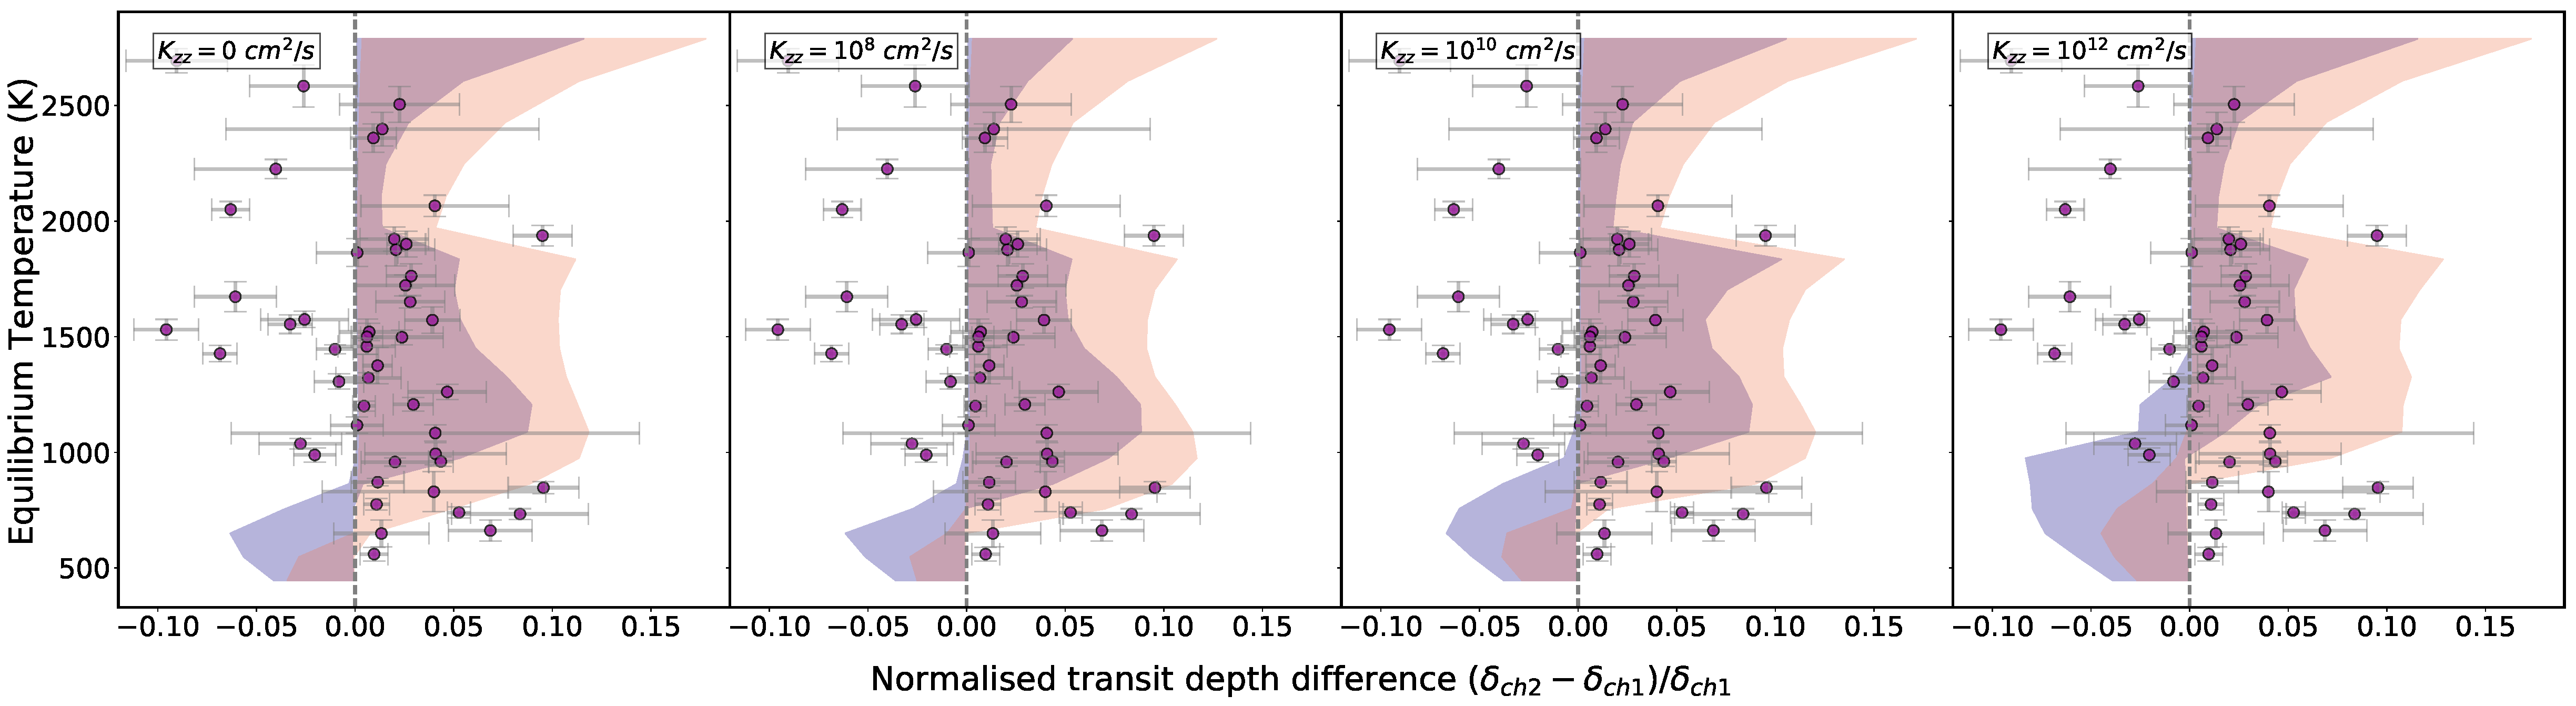
\includegraphics[width=\textwidth]{Kzzmodels.pdf}
%     \caption{Normalised Spitzer transit depth difference as a function of the equilibrium temperature for the full grid of transmission models created with PLATON (\citep{Zhang2019}, see Section \ref{P1:sec:PLATON}). Panels from left to right show no vertical mixing, Kzz = 1e8, Kzz = 1e10 and Kzz = 1e12. First row shows the 1x solar composition and second row shows the 30x solar composition. Gray dashed line represents a gray opacity source showing no spectral features.}
%     \label{P1:fig:Kzz}
% \end{figure*}

    % \item Shami models
%Heng 2014 equation
% \begin{equation}
% \begin{split}
% \bar{T}^4 =& \frac{T_{\rm int}^4}{4} \left[ \frac{1}{\epsilon_{\rm L}} + \frac{m}{\epsilon_{\rm L_3} \beta^2_{\rm L_0}} \left( \kappa_0 + \frac{\kappa_{\rm CIA} m}{2 m_0} \right) \right] \\
% &+ \frac{T_{\rm irr}^4}{8} \left[ \frac{1}{2 \epsilon_{\rm L}} + {\cal E}_2 \left( \frac{\kappa_{\rm S}}{\kappa_{\rm L} \beta_{\rm S_0}} - \frac{\kappa_{\rm CIA} m \beta_{\rm S_0}}{\epsilon_{\rm L_3} \kappa_{\rm S} m_0 \beta_{\rm L_0}^2} \right) \right.\\
% &\left.+ \frac{\kappa_0\beta_{\rm S_0}}{\epsilon_{\rm L_3} \kappa_{\rm S}\beta_{\rm L_0}^2} \left( \frac{1}{3} - {\cal E}_4 \right) + \frac{\kappa_{\rm CIA} \beta_{\rm S_0}^2}{\epsilon_{\rm L_3} \kappa_{\rm S}^2 m_0 \beta_{\rm L_0}^2} \left( \frac{1}{2} - {\cal E}_3 \right) \right].
% \end{split}
% \label{P1:eq:heng}
% \end{equation}
%     \item Mike models
%     \item Equilibrium chemistry vs non-equilibrium
%     \item Effect of the star/photochemistry
% \end{itemize}

\section{Exoplanet atmosphere diversity}

%From the first exoplanet discovery in

% Spitzer/Infrared Array Camera (IRAC) \citep[e.g.,]{Knutson2008, Line2014}, Hubble Space Telescope (HST)/Wide Field Camera 3 (WFC3) \citep[e.g.,][]{Kreidberg2015, Kreidberg2018b, Arcangeli2018}, HST/Space Telescope Imaging Spectrograph (STIS) \citep[e.g.,][]{Charbonneau2002}, and several ground based observatories \citep[e.g.,][]{Swain2010, Sing2011, Huitson2017}.

The last 30 years of exoplanet research has seen the field progress from the first exoplanet detection \citep{Mayor1995}, through to the detection of the first exoplanetary atmosphere \citep{Charbonneau2002} and to the cataloging of thousands of exoplanets (e.g. \citet{Borucki2010, Batalha2013}). Having categorized these planets (e.g. hot Jupiters, warm-Neptunes, and terrestrial planets), the field currently focuses on assessing their characteristics using space and ground-based spectroscopy/photometry. We are now in a realm of comparative exoplanetology. This thesis comprises the largest survey of the emission of exoplanets as well as the largest survey in transmission with Spitzer/IRAC. The following section will discuss some of the notable survey results from the literature.

% From the first exoplanet discovery in 1995 to the first measurement of at atmosphere with Spitzer/IRAC in 2005 we are now in a realm of comparative exoplanetology.

%, ranging from %cool gas giants \citep{Wallack2019},
%warm-neptunes  to
%hot Jupiters .
%and with \citep{Heng2016}
%and ultra-hot Jupiters \citep{Baxter2020}.

\subsection{Looking at planet ensembles}

% Transmission surveys

\subsubsection{Transmission surveys}


In recent years, there have been several studies exploring the trends in HST/WFC3 transmission spectra of warm-Neptunes \citep{Crossfield2017} and hot Jupiters \citep{Stevenson2016a, Sing2016, Heng2016, Barstow2017, Fu2017, Tsiaras2018}. Notably, \citet{Sing2016} performed a survey of 10 transiting planets using HST/STIS (which probes the alkali lines and the Rayleigh slope), HST/WFC3 (which probes the 1.4~\um~ water feature), and Spitzer/IRAC (which probes \ce{CH4} and CO). They find that their sample of hot Jupiters is extremely diverse, exhibiting a continuum from the clear to cloudy atmospheres, see Figure \ref{int:fig:singetal}. They define a metric based on the difference in the transit depth measured in the infrared vs the optical wavelengths. They note that it correlates with the spectral strength of the water feature, indicating that this metric can be used to classify objects.  \citet{Stevenson2016b} similarly creates a metric for measuring the strength of the water feature using HST/WFC3 spectra and finds that it strongly correlates with planet temperature, implying that cooler atmospheres below 700K are likely to have dampened features due to clouds. Around the same time, \citet{Heng2016} creates a dimensionless cloudiness index for a sub-sample of 7 planets from \citet{Sing2016}. Their index is based on the sodium and potassium lines of these planets and thus probing smaller particles than the metric of  \citet{Stevenson2016b}, yet they still find a tentative decreasing cloudiness trend with increasing equilibrium temperature. Additionally, \citet{Crossfield2017} studied a sample of 6 warm-Neptunes with HST/WFC3 observations and found a correlation with the spectral features and the equilibrium temperature suggesting more optically thick clouds at lower temperatures.


\begin{figure}
    \centering
    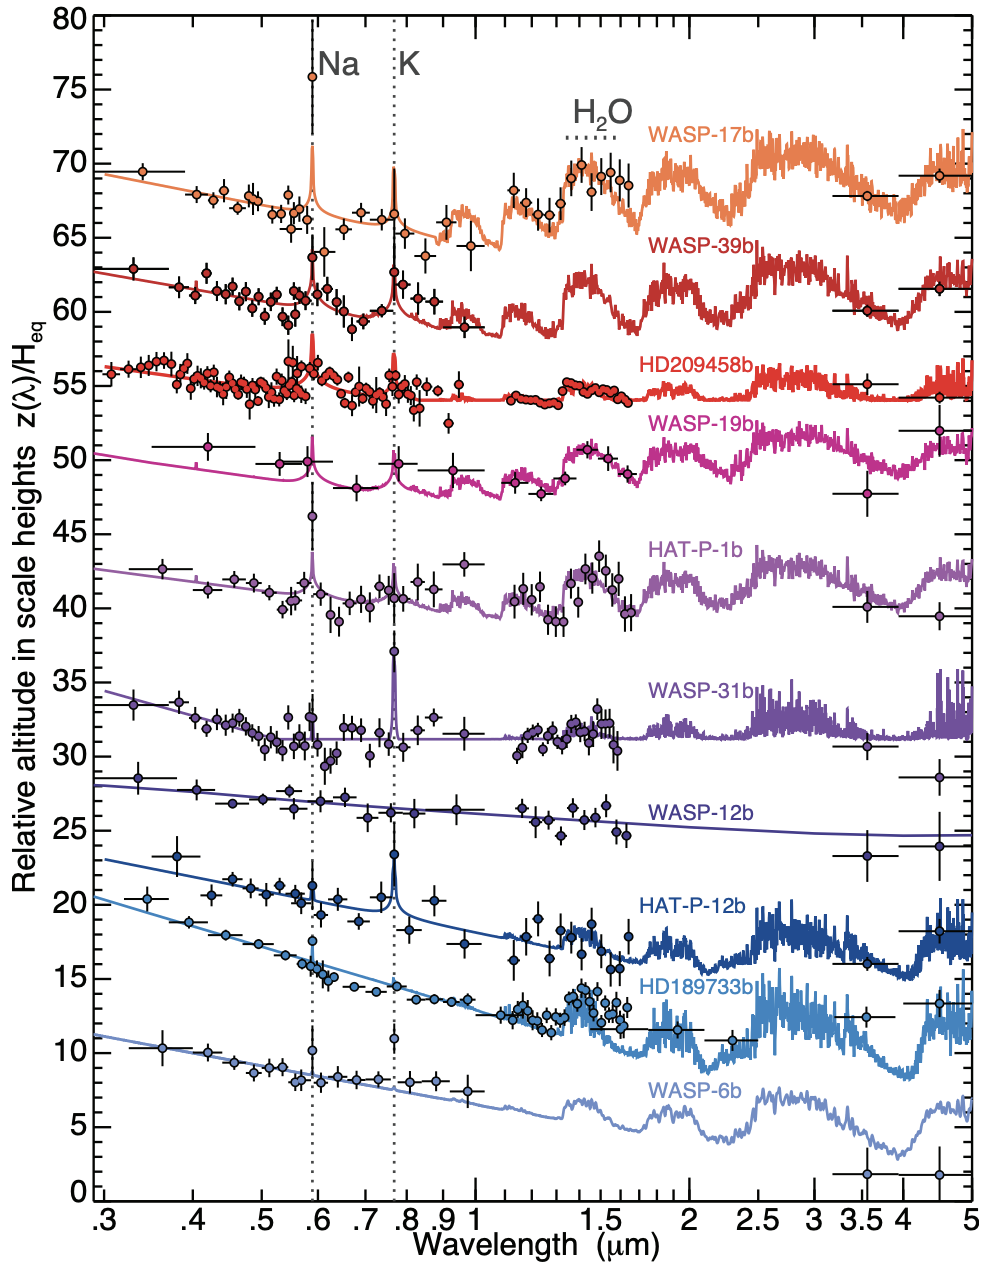
\includegraphics[width = \linewidth]{singetal.png}
    \caption{HST and Spitzer transmission spectra of 10 hot Jupiters. Solid colored lines show fitted atmospheric transmission spectra models where the alkali lines and the water feature are noted. The spectra are ordered in terms of their cloudiness, with the clear atmospheres appearing at the top of the image. The 3.6 and 4.5~\um~ Spitzer/IRAC transit depths probe the \ce{CH4} and CO molecular features respectively. Image credit: \citet{Sing2016}}
    \label{int:fig:singetal}
\end{figure}

\citet{Barstow2017} performed a consistent retrieval of the 10 hot Jupiters presented in \citet{Sing2016}, finding that the planets between 1300-1700K are represented with deeper grayer clouds or clear atmospheres and the rest, cooler or hotter, are better with high altitude hazes causing Rayleigh scattering. And finally, \citet{Fu2017} collected all HST/WFC3 observations of 34 gas giants and compared them with a forward model for each planet calculated using Exo-Transmit. They found a negative slope in the absorption in scale heights vs equilibrium temperature which they attributed to decreasing cloudiness with increasing temperature.

Similar to these works, in Chapter \ref{transits} we use the normalized difference between the two Spitzer infrared bandpasses to classify the chemical composition of the atmospheres of our sample. We tested how our metric correlates with all system parameters of the data and used it to compare our novel grids of forward models to the data. Finally, we incorporated important effects such as varying composition and disequilibrium chemistry into our modelling and compared the model grids with the data over a large range of system parameters.

\subsubsection{Emission surveys}

% Emission Surveys
There has also been a lot of work done studying the atmospheres of surveys of exoplanets by measuring the emission from their daysides. Despite the extreme differences in the amount of insolation they receive, hot Jupiters have similar equilibrium temperatures to late-type brown dwarfs. There have been several studies looking at the color-color and color-magnitude diagrams of exoplanets \citep{Triaud2014a, Triaud2014c, Dransfield2020, Melville2020}. \citet{Triaud2014c} calculate color-magnitude diagrams of a survey of 44 exoplanets using photometric distances and WISE magnitudes in combination with Spitzer emission in the four bandpasses (3.6, 4.5, 5.8, and 8.0~$\mu$m). Figure \ref{int:fig:triaud} displays the color-magnitude diagrams for the warm-Spitzer bandpasses. These figures show increasing scatter with increasing magnitude, which \citet{Triaud2014c} attributes to increased atmospheric diversity at colder temperatures. Furthermore, they found that hot Jupiters have colors similar to brown dwarf (MLT) colors i.e., these planets do not have simply featureless spectra in the infrared. It is likely though, that these similar colors are due to different processes in the atmospheres of hot Jupiters and brown dwarfs.

\begin{figure}
    \centering
    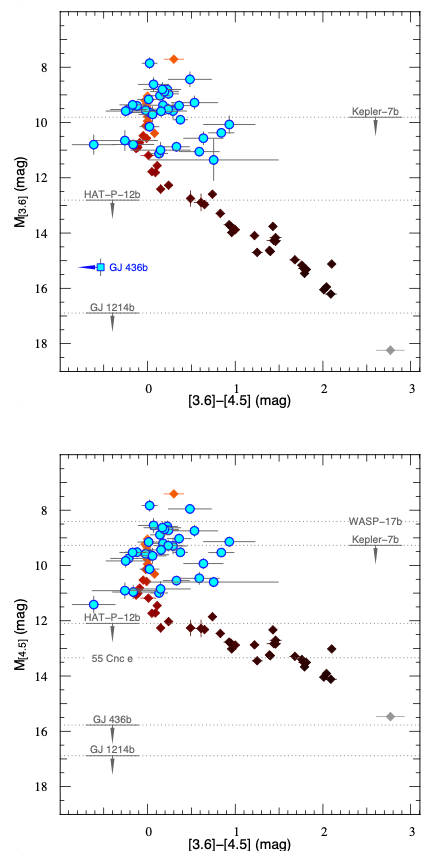
\includegraphics[height = \textheight]{triaud.png}
    \caption{Color-magnitude diagrams using the warm-Spitzer bandpasses. Blue dots show the planetary magnitudes and colors calculated from the secondary eclipse measurements. The colored diamonds show the magnitudes of ultra-cool brown dwarfs whose values were taken from \citet{Dupuy2012}. Image Credit: \citet{Triaud2014c}.}
    \label{int:fig:triaud}
\end{figure}

Additional studies have focused on using the infrared Spitzer emission observations to constrain the energy budgets of hot Jupiters. \citet{Schwartz2015} calculated the dayside effective temperature of a survey of 50 planets with thermal emission measurements in at least two infrared wavelengths (>0.8~$\mu$m). They compared the dayside effective temperature ($T_{\rm eff}$) with the irradiation temperature ($T_0$). If there is full redistribution of stellar irradiation then the effective dayside temperature will be the equilibrium temperature, where $T_{eq,\textit{0}} = (1/4)^{1/4} T_0 \approx 0.71T_0$. They found that the daysides of hotter planets deviate further from equilibrium temperature estimations, implying that the hotter planets do not redistribute heat as efficiently from their day to nightsides. This supports the previous claim by \citet{Cowan2011b} that the hottest planets have lower Bond albedo and/or less efficient heat transport, and is in agreement with theoretical predictions about redistribution efficiency in \citet{Perez-Becker2013}. However, \citet{Schwartz2017} incorporated phase offsets into their energy budget calculations of six planets, which pushes the results for these planets toward the lower Bond albedos scenario with slightly higher heat transport than previous measurements.

Furthermore, \citet{Garhart2020} performed a uniform analysis of 36 planets with Spitzer/IRAC secondary eclipses measured at 3.6 and 4.5~$\mu$m. They calculated the brightness temperatures and found an increasing trend in the brightness temperature ratio with equilibrium temperature. In Chapter \ref{eclipses} we use these results in combination with 42 other planets with both 3.6 and 4.5~$\mu$m emission measurements to study how the dayside emission changes between the hot and the ultra-hot Jupiters. We revisit the trends seen in \citet{Schwartz2015} and \citet{Garhart2020} with our expanded survey of 78 planets in emission. When we carefully analyzed and calculated  the brightness temperatures, we found that the trend with dayside temperature and irradiation temperature is less significant than before when you properly incorporate a stellar model instead of a blackbody for the star.
%Furthermore, typically the effective temperature is calculated by fitting a blackbody to the spectral energy distribution of the planet. In this case, there are just two photometric points, one of which has a strong CO emission feature (4.5~\um~). Therefore, calculating the effective temperature as a weighted mean of the two Spitzer brightness temperatures can bias the effective temperature results towards hotter temperatures. We suggest that the dayside effective temperature is better approximated with just the 3.6~\um~ brightness temperature, as this probes closer to the continuum. When this is done, the trend suggesting lower redistribution efficiency with hotter planets is no longer statistically significant. However, there remains a large scatter in the brightness temperatures of hotter planets compared to cooler planets, which could suggest a range of redistribution efficiencies for the hottest planets.
Additionally, in Chapter \ref{transits} we revisit the color-magnitude diagrams of \citet{Triaud2014} with our expanded survey in combination with GAIA data release 2 distances and find that the larger sample is in agreement with previous works.

\subsection{The Ultra-hot Jupiters as a separate class}

Ultra-hot Jupiters are the newest class of exoplanets, it was only in the last few years that their atmospheres started to be understood \citep[e.g.,][]{Arcangeli2018, Parmentier2018b, Lothringer2018, Kitzmann2018}. Previously, emission spectra of these ultra-hot planets appeared to be blackbodies and the abundances retrieved from model fitting were very different from the general population of hot Jupiters \citep{Stevenson2014b, Haynes2015,Evans2017,Sheppard2017}. Retrieved abundances were driven in part by the strong CO feature seen with Spitzer/IRAC and the lack of \ce{H2O} feature at the HST/WFC3 wavelengths. This resulted in high retrieved C/O ratios, which would have required most of the oxygen to be locked up in CO leaving very little to form \ce{H2O}. These high C/O ratios lead to questions regarding formation, why should the ultra-hot planets differ in metallicity from their cooler counterparts? In \citet{Arcangeli2018} they explored the effect of molecular dissociation of molecules such as \ce{H2O} and TiO, as well as the recombination of H atoms with electrons to form H-, and found that when including these effects they were able to explain the emission spectra without the need to invoke very high metallicity (see Figure \ref{int:fig:w18}). The H- continuum opacity dominates the spectrum at the HST/WFC3 wavelengths and fills in the gap at 1.3~\um~ while we see the bump of \ce{H2O} in emission at 1.5~\um~, making the spectrum appear like a blackbody.

Furthermore, with TiO and VO dissociated on the dayside, there still remained temperature inversions in model atmospheres of ultra-hot Jupiters, which were due to the strong absorption of atomic metals (Fe, Mg), SiO, and metal hydrides such as FeH \citep{Lothringer2018}. Observations of temperature inversions in hot Jupiters were notoriously hard to find, with only hints of emission in the Spitzer bandpasses in a few planets \citep[e.g.,][]{Nymeyer2011, Deming2012}. However, there have now been a few observations of inversions in the ultra-hot Jupiters: WASP-33b, WASP-121b, and WASP-18b (Figure \ref{int:fig:w18}) \citep{Haynes2015, vonEssen2015, Evans2017, Arcangeli2018, Kreidberg2018b}. It is in this context that in Chapter \ref{eclipses}, we look at how the dayside emission in the two Spitzer bandpasses changes as the temperature of the planets increases. We find a transition at 1700K, which is likely caused by temperature inversions resulting in a strong CO feature appearing in emission.

As is mentioned in Section \ref{int:sec:variability}, the extreme atmospheres of ultra-hot Jupiters, in particular the high degree of ionization due to the intense stellar irradiation, could result in the dayside emission being variable in time. Additionally, the effects of dissociation and recombination of \ce{H2} were studied in \citet{Komacek2018b} and \citet{Bell2018}, where it was discovered that recombination of atomic hydrogen occurs when it is transported from the hot dayside to the cooler nightside of these planets. This recombination releases a significant amount of heat that can warm up the nightside of the planet, increasing the global efficiency of heat redistribution \citep{Mansfield2020}. This result is in contrast with previous suggestions of lower efficiency of heat redistribution in the hottest planets and might be why we do not see this trend in the brightness temperatures measured in Chapter \ref{eclipses}. Additionally, dissociation and recombination and transport between the day and nightsides could also be a cause of the variability that we see in the dayside of WASP-18b in Chapter \ref{w18b}.

\subsection{The cool planets}

In this thesis (Chapters \ref{transits} and \ref{TTVs}), we also study some of the coolest gas giants that we know of, with temperatures around 500K. However, cooler exoplanets have lower signal-to-noise ratio both in transmission and emission, making their atmospheres extremely difficult to characterize. There have been several studies focusing on the characterization of individual cool gas-giant exoplanets. Notably, the atmosphere of the Neptune mass planet, GJ436b, has been studied on many occasions in both emission and transmission with HST and Spitzer/IRAC \citep{Deming2007, Demory2007, Gillon2007a, Gillon2007b, Stevenson2010a, Beaulieu2011, Knutson2011, Lanotte2014, Knutson2014a, Morley2017}. With an equilibrium temperature of 670K, chemical equilibrium models would predict that the atmosphere would have a high \ce{CH4} abundance, however, the atmosphere of GJ436b was shown to be substantially methane deficient \citep{Stevenson2010a, Knutson2011, Lanotte2014}. Furthermore, methane depletion compared to equilibrium chemistry expectations has been observed in many other warm giant planets with HST observations, e.g., WASP-107b and WASP-117 b \citep{Kreidberg2018a, Spake2018} or combined HST and Spitzer e.g., GJ3470 b \citep{Benneke2019}, HAT-P-11 b \citep{Chachan2019}, HAT-P-26 b \citep{Wakeford2017}, and WASP-39 b \citep{Wakeford2018}.

\citet{Kammer2015} performed a small uniform survey of 5 cool gas giant planets (HAT-P-19b, WASP-6b, WASP-10b, WASP-39b, WASP-67b) with Spitzer/IRAC 3.6 and 4.5~\um~ and found a tentative correlation in the brightness temperature ratio and planet mass. They did not discover a trend with the equilibrium temperature. However, in Chapter \ref{eclipses} we look for trends with the brightness temperature ratio against equilibrium temperature against the whole sample of planets in emission, including those from \citet{Kammer2015}, and compare to models.
We do find a trend with equilibrium temperature and brightness temperature ratio throughout the entire range of temperatures. However, notably, the models suggest that there is a trend with brightness temperature ratio and equilibrium temperature of the coolest planets. This trend is also highly dependent on the metallicity of the host star and can switch between being correlated when [M/H] = 1 to anti-correlated when [M/H] = -1, see Figure \ref{int:fig:Tbratio}. Furthermore, \citet{Wallack2019} present an analysis of 5 more cool gas giants (HAT-P-15b, HAT-P-17b, HAT-P-18b, HAT-P-26b, and WASP-69b) and find a tentative trend with \ce{CH4}/(CO +\ce{CO2}) ratio and stellar metallicity, which is in agreement with our models.

\begin{figure}
    \centering
    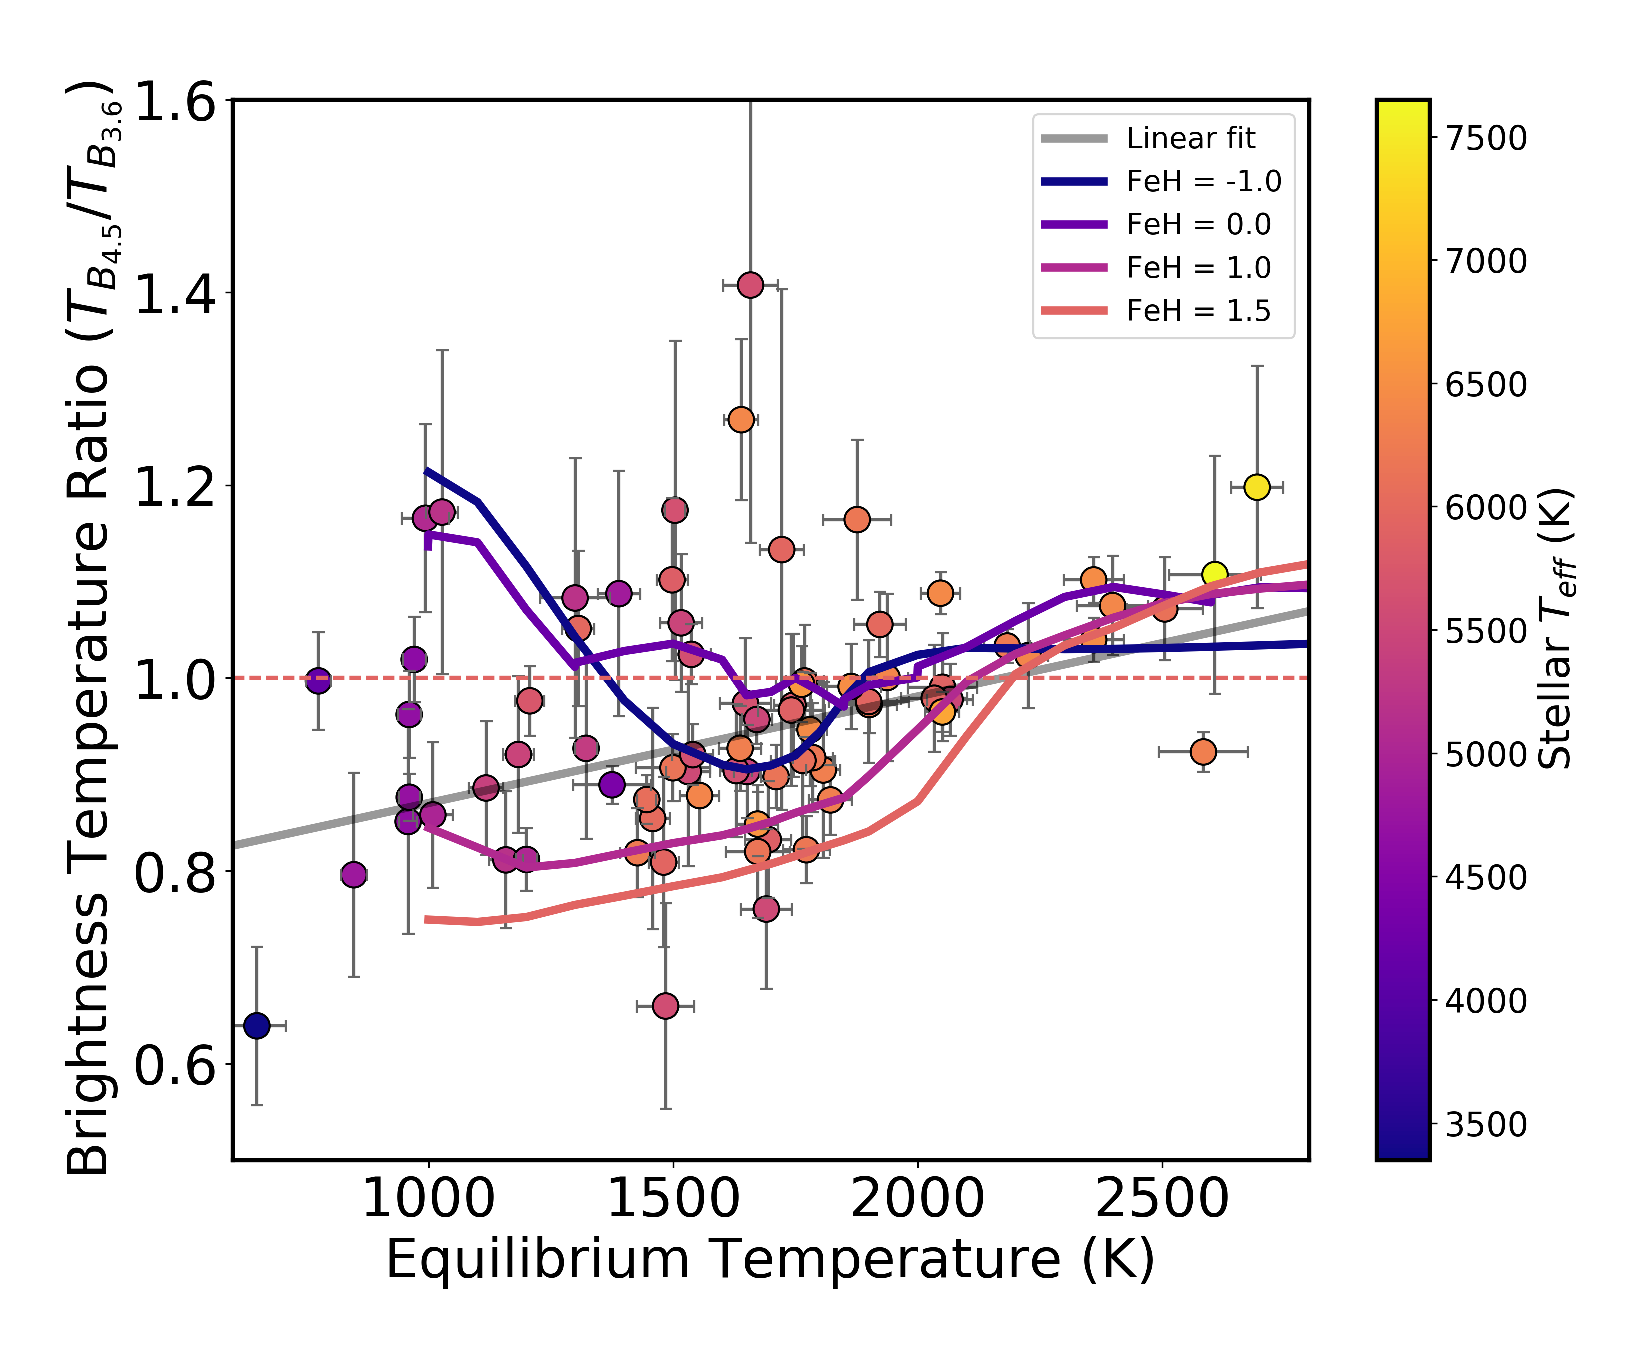
\includegraphics[width = \linewidth]{TbratiovsTeq_PHOENIX_intpl_wlabels.pdf}
    \caption{Brightness temperature ratio from Spitzer/IRAC observations of our survey of 78 planets plotted against the equilibrium temperature. Remake of Figure 4 of Chapter \ref{eclipses} except the grids of models are not interpolated over all parameters, instead we show the tracks for the different metallicities of the host star, which is the largest contributing factor to the spread of the models. The different metallicities indicate both a positive and a negative correlation with ratio of brightness temperatures of the the coolest planets against their equilibrium temperature depending on host star metallicity. }
    \label{int:fig:Tbratio}
\end{figure}


Several theories have been discussed to explain the lack of methane in the coolest hot Jupiters: including using non-equilibrium photochemical models \citep{Line2011}, models with hydrogen depletion \citep{Hu2015}, invoking tidal heating due to high eccentricity \citep{Agundez2014} and finally, high metallicity models (230-1000x solar) \citep{Moses2013b}. Additionally, the trend of brightness temperature against mass from \citet{Kammer2015} and against stellar metallicity from \citet{Wallack2017} all suggest a link between the atmospheric composition and planetary formation scenarios.

Predictions based on the chemical composition of the protoplanetary disks suggest that planets formed close-in to have low C/O ratios \citep[e.g.,][]{Oberg2011,Eistrup2018}. However, there has been evidence for planets having super-solar C/O ratios (C/O > 0.54) \citep[e.g.,][]{Lodders2004,Madhusudhan2011}, with interesting implications for their formation scenarios. In Chapter \ref{eclipses} we compare the sample of 78 planets in emission with a grid of models spanning different regions of parameter space. One of these parameters is the C/O ratio of the planetary atmosphere. We find that our sample of 78 planets statistically disfavors the models with high C/O ratios (C/O = 0.85).

% \subsection{Atmospheres as a tracer of formation}

% The atmospheres of all four of the Solar system gas giant planets have metallicities that are enhanced compared to the Sun. Spectroscopy of these atmospheres results in carbon abundances that show an enrichment factor of $\sim$4, 10, 80, and 80, for Jupiter, Saturn, Uranus, and Neptune, respectively. This was understood using the core accretion model of planetary formation \citep{Pollack1996} i.e. once a solid core reaches 10 earth masses this core will accrete solids and gas from the midplane of the protoplanetary disk. The local composition of this disk determines the atmospheric composition of the planet. Therefore, measuring the atmospheric abundances can help us constrain the chemistry, location and density of the disk where the planet formed \citep[e.g.,][]{Lodders2004,Oberg2011}.

% \citet{Oberg2011} suggested that the role of snow lines of \ce{H2O}, \ce{CO2} and CO can create distinct changes in the local carbon to oxygen ratio of the planet-forming disk, and therefore the C/O ratio of an exoplanet atmosphere can allow us to further distinguish between different formation locations and migration histories. \citet{Eistrup2018} shows a more complete picture by incorporating changes in the disk throughout its lifetime, yet distinct predictions on the C/O ratio based on radial distance and age are still expected. Based on these works, one would expect that planets formed close-in to have low C/O ratios, however, there has been evidence for planets having super-solar C/O ratios (C/O > 0.54) \citep[e.g.,][]{Lodders2004,Madhusudhan2011}, which could lead to questions about their formation scenarios. In Chapter \ref{} we compare the sample of 78 planets in emission with a grid of models spanning different regions of parameter space, one of these parameters is the C/O ratio of the planet atmosphere. We find that our sample of 78 planets statistically disfavours the models with high C/O ratios (C/O = 0.85).

% \section{Miscellaneous}

\section{This Thesis} %forward looking

This thesis focuses on the statistical characterization of exoplanet atmospheres in the infrared using the Spitzer Space Telescope.

Chapter \ref{transits} presents the data analysis pipeline used and augmented throughout the different chapters of this thesis. We reduce the data and simultaneously fit the transit parameters \citep[using Batman;][]{Kreidberg2015} with a pixel level decorrelation model and temporal ramp, and we create an automated search through all of the parameter space to determine the optimum background correction, centroiding, and photometric methods for the reduction. We use the pipeline to uniformly analyse a survey of 49 planets in transmission at 3.6 and 4.5~\um. Using these two wavelengths, we then define a model-independent metric for characterizing the atmospheric composition (probing the relative abundance of \ce{CH4} and \ce{CO}). We search for statistical trends using this Spitzer metric as a function of other planetary and stellar parameters. We hone in on how the equilibrium temperature plays a role in determining the chemistry of the atmosphere and the strength of the Spitzer metric. Finally, we compare the entire survey to custom grids of forward models containing important disequilibrium chemistry and varying metallicities.

Chapter \ref{eclipses} presents a survey of 78 gas giant exoplanets in emission. Using the eclipse depths at 3.6 and 4.5~\um, we carefully calculate the brightness temperatures by integrating properly over the Spitzer spectral response functions and by including a PHOENIX model for the stellar flux. We search for trends in the brightness temperatures and define a new metric for characterizing the dayside emission of the planets, the deviation from a blackbody. Using this metric, we compare the sample to a comprehensive grid of self-consistent forward models, which contain temperature inversions and important phenomena for the ultra-hot Jupiters. Additionally, we alter our custom pipeline to analyse secondary eclipses and analyse the hottest ultra-hot Jupiter known, KELT-9b, and comment on how this planet fits into the population.

Chapter \ref{w18b} presents a focused look at one ultra-hot exoplanet in particular, WASP-18b. Using our custom data analysis pipeline, we analyse 10 almost consecutive eclipses at 4.5~\um~. We find a periodic signal in the brightness variability in time. We confirm the signal by performing different analyses of the data and then explore possible physical phenomena that could be responsible for a time variable brightness in the atmosphere.

Finally, Chapter \ref{TTVs} presents an analysis of seven of the coolest planets from our science exploration program. These planets are part of three multi-planet systems (Kepler-9, Kepler-18 and Kepler-32) and one circumbinary system (Kepler-16). Due to the low signal-to-noise of the multi-planet system planets, we alter the pipeline to extract only the transit times. We then compare the measured transit times to predictions made with timing variation models based on the original Kepler observations, which can help pin down the planetary masses. On the other hand, the signal-to-noise ratio of the Kepler-16b data is high, allowing us to extract exquisite transit lightcurves and to fit for the full range of transit parameters. We make predictions using a photo-dynamical model of the Kepler-16 system and compare this to the 3.6 and 4.5~\um transit lightcurves.


%%% Local Variables:
%%% mode:latex
%%% TeX-master: "../../thesis_renzo"
%%% End:
                          % introduction

\chapter[Evidence for disequilibrium chemistry from vertical mixing in hot Jupiter atmospheres: A comprehensive survey of transiting close-in gas giant exoplanets with warm-\spitzerIRAC]{Evidence for disequilibrium chemistry from vertical mixing in hot Jupiter atmospheres: A comprehensive survey of transiting close-in gas giant exoplanets with warm-\spitzerIRAC}
\chaptermark{Evidence for disequilibrium chemistry from vertical mixing in hot Jupiter atmospheres} %% if you want a different title in the headers
\label{transits}

%\subchapter{A comprehensive survey of transiting close-in gas giant exoplanets with warm-\spitzerIRAC}

% Define the location of your plots
\graphicspath{{./gfx/SpitzerStatisticalSurvey/}}

% List all paper authors
\chauthors{Claire Baxter,
          Jean-Michel D\'esert,
          Shang-Min Tsai,
          Kamen O. Todorov,
          Jacob L. Bean,
          Drake Deming,
          Vivien Parmentier,
          Jonathan J. Fortney,
          Michael Line,
          Daniel Thorngren,
          Raymond T. Pierrehumbert,
          Adam Burrows,
          Adam P. Showman}
\chjournal{Astronomy \& Astrophysics, 648, A127 (2021)}

\begin{abstract}
  % aims heading (mandatory)
  \textit{Aims} We present a large atmospheric study of 49 gas giant exoplanets using infra-red transmission photometry with \spitzerIRAC at 3.6 and 4.5~$\mu$m. \\
  % methods heading (mandatory)
   \textit{Methods} We uniformly analyse 70 photometric lightcurves of 33 transiting planets using our custom pipeline, which implements pixel level decorrelation. Augmenting our sample with 16 previously published exoplanets leads to a total of 49.
   We use this survey to understand how infra-red photometry traces changes in atmospheric chemical properties as a function of planetary temperature. We compare our measurements to a grid of 1-D radiative-convective equilibrium forward atmospheric models which include disequilibrium chemistry. We explore various strengths of vertical mixing ($K_{zz} = 0$ - $10^{12}$~\cmcms) as well as two chemical compositions (1x and 30x solar). \\
  % results heading (mandatory)
   \textit{Results} We find that on average, \spitzer probes a difference of 0.5 atmospheric scale heights between 3.6 and 4.5~$\mu$m, which is measured at $7.5~\sigma$ level of significance.
   Changes in the opacities in the two \spitzer bandpasses are expected with increasing temperature due to the transition from methane dominated to carbon monoxide dominated atmospheres at chemical equilibrium.
   Comparing the data with our model grids, we find that the coolest planets show a lack of methane compared to expectations, which has also been reported by previous studies of individual objects. We show that the sample of coolest planets rule out 1x solar composition with >$3~\sigma$ confidence while supporting low vertical mixing ($K_{zz} = 10^8$~\cmcms). On the other hand, we find that the hot planets are best explained by 1x solar metallicity and high vertical mixing models ($K_{zz}= 10^{12}$~\cmcms). We interpret this as the lofting of \ce{CH4} to the upper atmospheric layers. Changing the interior temperature changes the expectation for equilibrium chemistry in deep layers, hence the expectation from disequilibrium chemistry higher up. We also find a significant scatter in the transmission signatures of the mid-temperate and ultra-hot planets, likely due to increased atmospheric diversity, without the need to invoke higher metallicities. Additionally, we compare \spitzer transmission with emission in the same bandpasses for the same planets and find no evidence for any correlation.
   Although more advanced modelling would test our conclusions further, our simple generic model grid points towards different amounts of vertical mixing occurring across the temperature range of hot Jupiters. This finding also agrees with the observed scatter with increasing planetary magnitude seen in \spitzerIRAC color-magnitude diagrams for planets and brown dwarfs.
\end{abstract}


\section{Introduction}

\label{P1:sec:introduction}


Studying exoplanets is critical for gaining insights into the dominant composition and physical atmospheric processes and for understanding the theory of planet formation and evolution \citep{Seager2010, Crossfield2015, Deming2017}. Hot Jupiters with large scale heights are ideal targets for detecting molecular signatures in their atmospheres via transmission spectroscopy \citep{Seager2000a, Brown2001}. The atmospheres of such planets have been studied across a large range of wavelengths with a myriad of different instruments. Given the number of exoplanet atmospheres already observed, we now enter the era of statistical study of exoplanet atmospheres \citep[e.g.,][]{Triaud2014c, Beatty2014, Gao2020, Keating2019, Garhart2020, Baxter2020, Fu2017, Tsiaras2018, Wallack2019}.

Wavelength dependent transit depths are in principle primarily sensitive to the atmospheric composition \citep{Seager2000a}, in practice these observations have often been plagued by the presence of clouds/hazes dampening the expected molecular signals \citep[e.g.,][]{Fortney2005, Sing2016, Barstow2017}. Nevertheless, cloud-free hot Jupiter atmospheres in chemical equilibrium are predicted to exhibit traces of water, carbon monoxide and methane \citep{Seager2000b, Fortney2005, Fortney2010}. Studies are conducted to demonstrate whether such elements are statistically and systematically observed in exoplanets \citep{Tsai2018}. However, non-equilibrium chemistry and clouds are predicted to be present in close-in giant exoplanet atmospheres, and will impact their observations \citep[e.g.,][]{Agundez2012, Drummond2016, Steinrueck2019}. \citet{Sing2016} performed a mini-survey of the transmission spectra of ten hot Jupiters. They characterize them in terms of a cloud index and find a transition between cloudy and cloud-free atmospheres. They note that a temperature-pressure profile crossing a condensation curve is not solely responsible for the resulting dampened spectra, rather it is likely that non-equilibrium effects such as atmospheric circulation and vertical mixing play a role.

There are several important atmospheric processes to consider that can drive atmospheres away from cloud-free chemical equilibrium. \citet{Zhang2018a} showed that atmospheric transport can move atmospheric abundances away from chemical equilibrium and greatly alter the expected spectroscopic observations. They develop a 1D framework to capture these complex atmospheric processes and parameterize it with an eddy diffusion co-efficient ($K_{zz}$). For hot Jupiters, $K_{zz}$ ranges from $10^8$ to $10^{12}$~\cmcms, based on the estimation of the mean vertical wind in global circulation models (GCM) \citep{Moses2011, Parmentier2013}. Additionally, \citet{Komacek2019} estimated that the strength of vertical mixing will increase for hotter planets. Particularly relevant to this work is the recent advances made in the field of brown dwarf atmospheres: \citet{Miles2020} study the strength of vertical mixing in cool brown dwarf atmospheres with temperatures 250-750~K, and find that the cooler objects support mixing close to the theoretical maximum yet the warmer objects show weaker than predicted mixing.


Additionally, the atmospheres of warm giant close-in exoplanets seem to be deficient in methane. According to equilibrium chemistry, methane is predicted to be abundant in the atmospheres of exoplanets with equilibrium temperatures cooler than 1100~K \citep{Madhusudhan2012}. In this context, \citep{Stevenson2010a} showed that the atmosphere of GJ436b is substantially methane deficient relative to chemical equilibrium models, suggesting the presence of non-equilibrium processes such as those induced by vertical mixing, which has been tested by follow-up studies \citep{Knutson2011, Lanotte2014}. Several other studies have attempted to model the methane depletion of GJ 436b: using non-equilibrium photochemical models \citep{Line2011}, high metallicity (230-1000x solar) models \citep{Moses2013b}, models with hydrogen depletion \citep{Hu2015}, and invoking tidal heating due to high eccentricity \citep{Agundez2014}. \citet{Morley2017} provide new data along with a reanalysis and new modeling, they confirm the methane depletion and find the best fitting models have high metallicity, disequilibrium chemistry and tidal heating resulting in an intrinsic temperature ($T_{\rm int}$) of 300-350~K. $T_{\rm int}$ characterizes the heat flux escaping from the planetary interior, which is written as $\sigma T_{\rm int}^4$. Recently, \citet{Fortney2020} suggested that the ongoing eccentricity damping of three warm Neptunes, including GJ 436b, heats their atmospheres and drives strong convective mixing resulting in a decreased \ce{CH4}/CO ratio.

Furthermore, methane depletion has been observed in a slew of other warm giant planets. HST/WFC3 observations of the transmission spectra of both WASP-107 b and WASP-117 b reveal no detection of methane expected from chemical equilibrium, only upper limits, suggesting a methane depletion in these atmospheres \citep{Kreidberg2018a, Spake2018, Carone2021}. Additionally, combined HST/WFC3 and \spitzerIRAC transmission spectra observations of GJ3470 b \citep{Benneke2019}, HAT-P-11 b \citep{Chachan2019}, HAT-P-26 b \citep{Wakeford2017} and WASP-39 b \citep{Wakeford2018} all have lower than expected abundances of methane given their temperatures. All in all, methane has only been sparsely detected in the atmospheres of a few exoplanets \citep{Swain2008,Tinetti2010,Guilluy2019}.

In this paper, we aim to statistically characterize a large sample of hot Jupiters using the two remaining active detectors on \spitzerIRAC at 3.6~$\mu$m. and 4.5~$\mu$m. \citep{Fazio2004, Werner2004}. At these two wavelengths we expect to see the absorption of methane (\ce{CH4}) and carbon monoxide or carbon dioxide (CO or \ce{CO2}) respectively. We uniformly analyze \spitzerIRAC photometric transit lightcurves of a survey of 34 gas giant planets. This survey represents the largest analysis of \spitzerIRAC observations of gas giants in transmission to date, and it spans equilibrium temperatures from 500~K to 2700~K.

This paper is organized as follows: In Section \ref{P1:sec:observations} we describe the observations and the survey of planets. In Section \ref{P1:sec:Analysis} we describe the data reduction, photometric extraction, lightcurve fitting, and the creation of our grid of 1-D atmospheric models. Section \ref{P1:sec:Results} describes the results for the transit survey and the statistical survey comparison to the grid of models. In Section \ref{P1:sec:Discussion} we discuss the context and implications for the different trends and statistics that we observe. Additionally, in Section \ref{P1:sec:Discussion} we describe the collection and combination of the secondary eclipse data with GAIA distances and discuss and comparison between transits and eclipses.

\section{Observations}

\label{P1:sec:observations}

As part of the survey programs 90092 (PI Desert) and 13044 (PI Deming) we present the transit depth analysis 70 transit lightcurves of 33 planets in the Post Cryogenic Warm \textit{\spitzer}/IRAC bandpasses of 3.6~$\mu$m and 4.5~$\mu$m. With the goal of gaining a stronger understanding of the origins and nature of the exoplanets already discovered, we designed the survey to probe a wide range of masses, radii and equilibrium temperatures: ranging from cooler long-period gas giants ($\sim200$K) from the \textit{Kepler} mission to close-in hot Jupiters (up to 2300~K). Table \ref{P1:tab:obs} presents the observational information for the 33 planets in the survey. These exoplanets were selected due to their high expected signal-to-noise ratio and, in the case of the Kepler planets, their multiplicity. Additionally, we augment this sample with two extra planets to probe the coolest and the hottest regions of parameter space, these are WASP-121b from program 13044 (PI Deming) and WASP-107b from program 13052 (PI Werner). A full list of the observations is displayed in Table \ref{P1:tab:obs}.

All observations from our survey were taken in "peak-up" mode. Meaning the main observation was preceded by a 30 minute peak-up observation allowing for accurate pointing and thus obtaining precise positioning of the target to within 0.1 pixels throughout the observations. This significantly reduces the ramp effect caused by the intrapixel sensitivity (discussed in Section \ref{P1:subsec:systematics}).

We expand our survey to other transiting planets for which the transit depths in the \spitzer bandpasses are taken from the literature. First, we perform a search on exoplanets.org \citep{Wright2011} which yielded 3.6~$\mu$m and 4.5~$\mu$m transits for 16 additional planets. Combining these with our survey allows us to gain insights into the current state of infrared exoplanet transmission spectra in a statistical manner. These additional planets and their transit depths are listed in Table \ref{P1:tab:littransits}. Figure \ref{P1:fig:planets} presents a visualization of the parameter space covered by all planets in our survey (analyzed and literature).

WASP-6b and WASP-34b are part of the original survey program 90092, however, we exclude them from our analysis because the transits were missed. In the case of WASP-6b, the predicted mid-transit times had a large degree of uncertainty on the ephemeris, and the observed transits in both channels did not have sufficient baseline to gain accurate constraints on the atmosphere. In the case of WASP-34b, both transits were missed due to an error in the ephemeris.

\begin{figure}
    \centering
    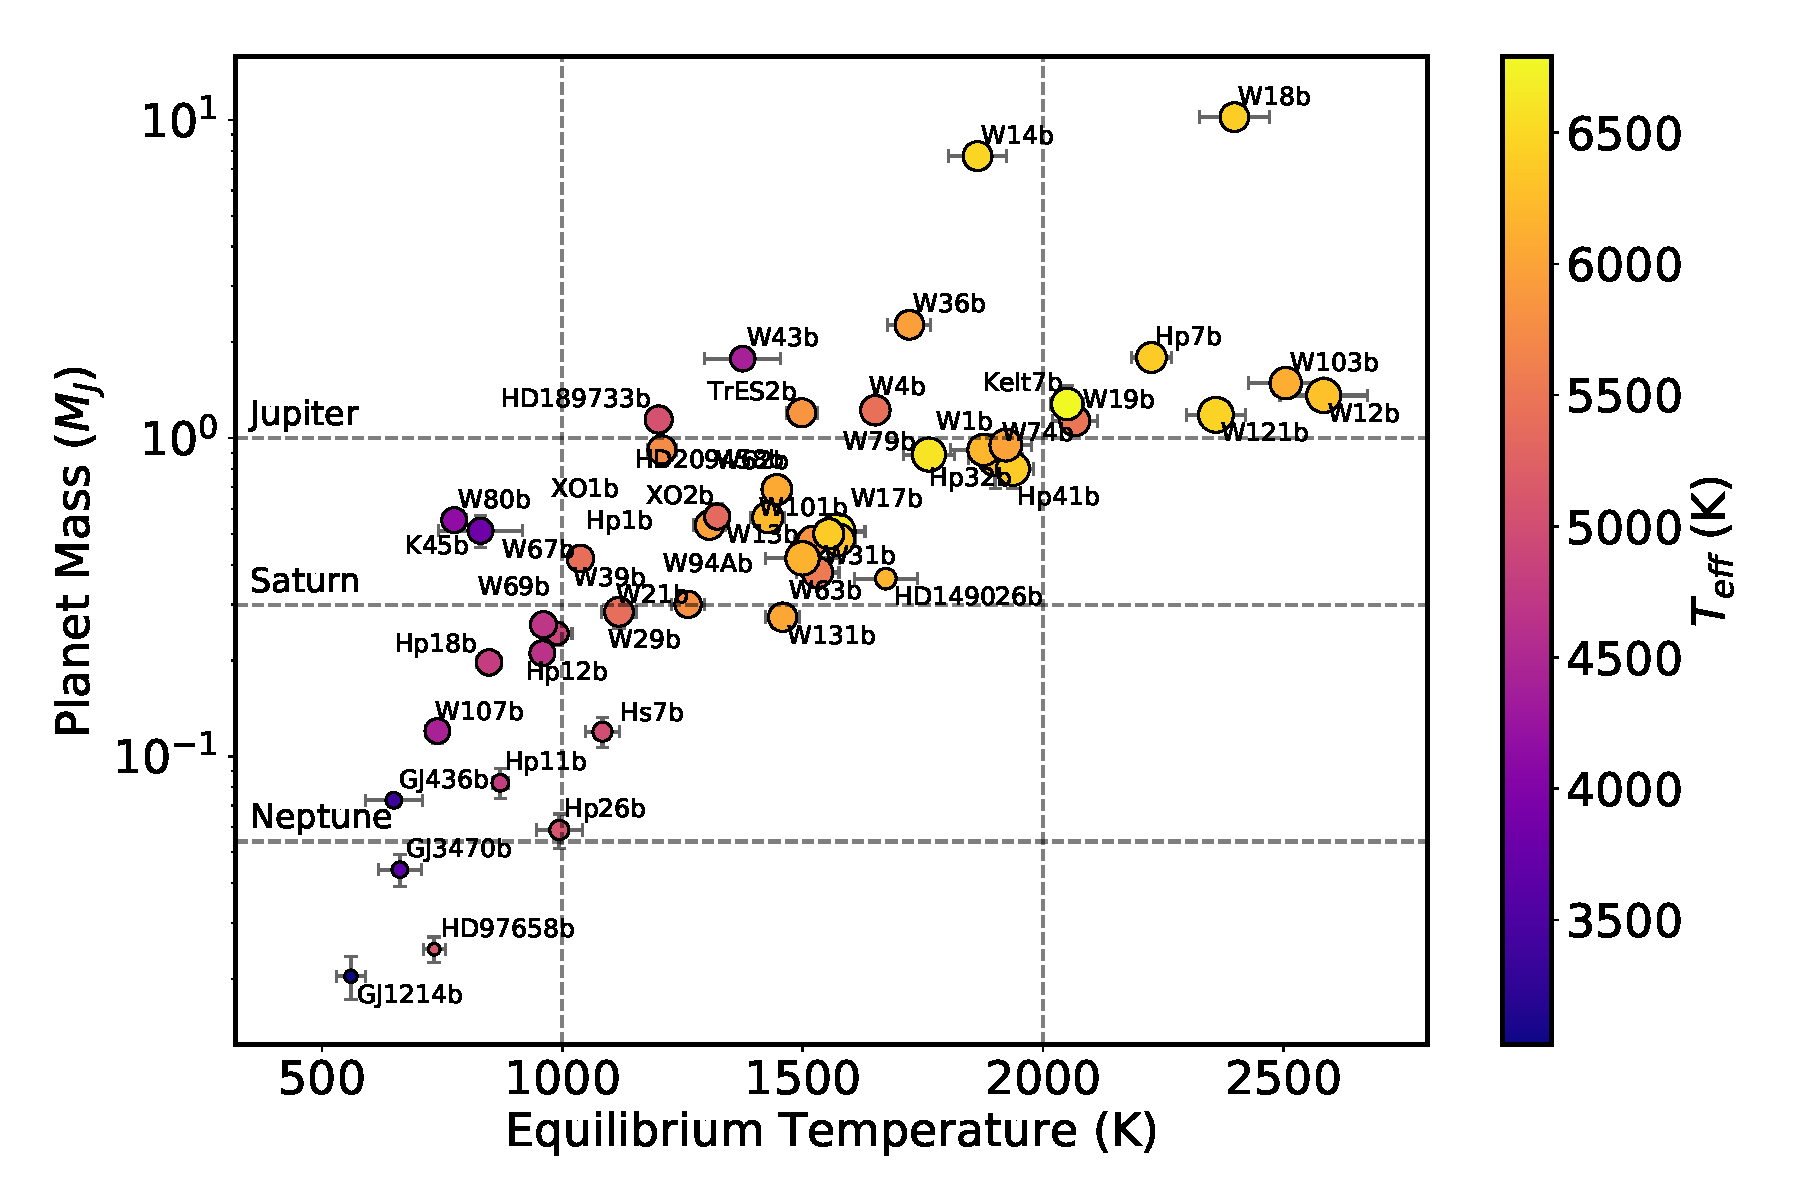
\includegraphics[width = \linewidth]{MassTemperature.pdf}
    \caption{Planet mass ($M_{jup}$) versus equilibrium temperature in Kelvin (assuming zero albedo and full redistribution) for all the planets presented in the current survey. The color of the points shows the stellar temperature ($T_{\rm eff}$) in Kelvin and the size of the points is scaled proportionately to the planetary radius. The gray dashed horizontal lines mark the masses of Jupiter, Saturn and Neptune. The gray dashed vertical lines mark the temperature regions discussed in Section \ref{P1:subsec:TDvsTeq}.}
    \label{P1:fig:planets}
\end{figure}


\begin{longtable}[h]{lllllll}

\caption{Details of the \spitzer Observations used in our survey analysis showing the UT date of observation, the duration of observation in hours, and the program ID of each transit. \label{P1:tab:obs}}\\

\hline\hline
Target & $\lambda$ & UT Start Date &  Duration &  Program ID\\
& $\mu$ m & & Hours &  \\
\hline
\endfirsthead
\caption{continued.} \\
\hline\hline
Target & $\lambda$ & UT Start Date &  Duration &  Program ID\\
& $\mu$ m & & Hours &  \\
\hline
\endhead
\hline
\endfoot

GJ3470 b    &               4.5 &   2013 Jan 01 &         4.4 &       90092 \\
GJ3470 b    &               3.6 &   2012 Dec 22 &         4.4 &       90092 \\
HAT-P-12 b  &               4.5 &   2013 Mar 11 &         4.5 &       90092 \\
HAT-P-12 b  &               3.6 &   2013 Mar 08 &         4.5 &       90092 \\
HAT-P-18 b  &               3.6 &   2013 Jun 17 &         5.0 &       90092 \\
HAT-P-18 b  &               4.5 &   2013 Jul 09 &         5.0 &       90092 \\
HAT-P-1 b   &               4.5 &   2013 Sep 20 &         5.2 &       90092 \\
HAT-P-1 b   &               3.6 &   2013 Sep 11 &         5.2 &       90092 \\
HAT-P-26 b  &               3.6 &   2013 Sep 09 &         4.5 &       90092 \\
HAT-P-26 b  &               4.5 &   2013 Apr 23 &         4.5 &       90092 \\
HAT-P-32 b   &               3.6 &   2012 Nov 18 &         5.4 &       90092 \\
HAT-P-32 b  &               4.5 &   2013 Mar 18 &         5.4 &       90092 \\
HAT-P-41 b   &               3.6 &   2017 Jan 18 &        12.1 &       13044 \\
HAT-P-41 b   &               4.5 &   2017 Feb 03 &        12.1 &       13044 \\
HATS-7 b     &               4.5 &   2016 Nov 04 &         5.2 &       13044 \\
HATS-7 b     &               3.6 &   2016 Nov 01 &         5.2 &       13044 \\
KELT-7 b     &               4.5 &   2017 Jan 04 &        10.3 &       13044 \\
KELT-7 b     &               3.6 &   2016 Dec 27 &        10.3 &       13044 \\
Kepler-45 b &               4.5 &   2013 Sep 29 &         4.5 &       90092 \\
Kepler-45 b &               3.6 &   2013 Sep 22 &         4.5 &       90092 \\
Kepler-45 b &               4.5 &   2013 Sep 12 &         4.5 &       90092 \\
Kepler-45 b &               3.6 &   2013 Sep 07 &         4.5 &       90092 \\
Kepler-45 b &               3.6 &   2013 Oct 16 &         4.5 &       90092 \\
Kepler-45 b &               4.5 &   2013 Nov 15 &         4.5 &       90092 \\
Kepler-45 b &               4.5 &   2013 Aug 21 &         4.5 &       90092 \\
Kepler-45 b &               3.6 &   2013 Aug 06 &         4.5 &       90092 \\
TrES-2 b     &               4.5 &   2012 Nov 26 &         4.3 &       90092 \\
TrES-2 b     &               3.6 &   2012 Nov 21 &         4.3 &       90092 \\
WASP-101 b   &               4.5 &   2017 Jan 17 &         8.0 &       13044 \\
WASP-101 b   &               3.6 &   2017 Jan 06 &         8.0 &       13044 \\
WASP-107 b  &               3.6 &   2017 May 02 &         8.7 &       13052 \\
WASP-107 b  &               4.5 &   2017 Apr 26 &         8.7 &       13052 \\
WASP-121 b   &               4.5 &   2017 Jun 05 &         8.5 &       13044 \\
WASP-121 b   &               3.6 &   2017 Jun 02 &         8.5 &       13044 \\
WASP-131 b   &               4.5 &   2017 Jun 04 &        11.3 &       13044 \\
WASP-131 b   &               3.6 &   2016 Nov 04 &        11.3 &       13044 \\
WASP-13 b   &               3.6 &   2013 Jul 07 &         7.5 &       90092 \\
WASP-13 b   &               4.5 &   2013 Jan 22 &         7.5 &       90092 \\
WASP-17 b   &               4.5 &   2013 May 14 &         8.2 &       90092 \\
WASP-17 b   &               3.6 &   2013 May 10 &         8.2 &       90092 \\
WASP-1 b    &               4.5 &   2013 Mar 20 &         6.8 &       90092 \\
WASP-1 b    &               3.6 &   2013 Mar 10 &         6.8 &       90092 \\
WASP-21 b   &               4.5 &   2013 Sep 01 &         6.1 &       90092 \\
WASP-21 b   &               3.6 &   2013 Aug 27 &         6.1 &       90092 \\
WASP-29 b    &               4.5 &   2017 Mar 14 &         7.8 &       13044 \\
WASP-29 b    &               3.6 &   2017 Feb 22 &         7.8 &       13044 \\
WASP-31 b   &               4.5 &   2013 Mar 19 &         4.6 &       90092 \\
WASP-31 b   &               3.6 &   2013 Mar 09 &         4.6 &       90092 \\
WASP-34 b   &               4.5 &   2013 Mar 25 &         4.5 &       90092 \\
WASP-34 b   &               3.6 &   2013 Mar 17 &         4.5 &       90092 \\
WASP-36 b    &               3.6 &   2017 Feb 20 &         7.3 &       13044 \\
WASP-36 b    &               4.5 &   2017 Aug 10 &         7.3 &       13044 \\
WASP-39 b   &               4.5 &   2013 Oct 10 &         5.0 &       90092 \\
WASP-39 b   &               3.6 &   2013 Apr 18 &         5.0 &       90092 \\
WASP-4 b    &               4.5 &   2012 Dec 31 &         4.3 &       90092 \\
WASP-4 b    &               3.6 &   2012 Dec 27 &         4.3 &       90092 \\
WASP-62 b    &               3.6 &   2016 Nov 24 &        11.3 &       13044 \\
WASP-62 b    &               4.5 &   2016 Dec 07 &        11.3 &       13044 \\
WASP-63 b    &               4.5 &   2017 Jun 17 &        15.8 &       13044 \\
WASP-63 b    &               3.6 &   2017 Apr 21 &        15.8 &       13044 \\
WASP-67 b    &               3.6 &   2017 Jan 22 &         5.6 &       13044 \\
WASP-67 b    &               4.5 &   2017 Aug 13 &         5.6 &       13044 \\
WASP-69 b    &               4.5 &   2017 Aug 30 &         6.5 &       13044 \\
WASP-69 b    &               3.6 &   2017 Aug 26 &         6.5 &       13044 \\
WASP-6 b    &               3.6 &   2013 Jan 21 &         4.6 &       90092 \\
WASP-6 b    &               4.5 &   2013 Jan 14 &         4.6 &       90092 \\
WASP-74 b    &               4.5 &   2017 Jan 16 &         6.7 &       13044 \\
WASP-74 b    &               3.6 &   2017 Jan 14 &         6.7 &       13044 \\
WASP-79 b    &               4.5 &   2016 Nov 27 &        11.1 &       13044 \\
WASP-79 b    &               3.6 &   2016 Nov 20 &        11.1 &       13044 \\
WASP-94 Ab   &               3.6 &   2017 Feb 10 &        13.3 &       13044 \\
WASP-94 Ab   &               4.5 &   2017 Aug 06 &        13.3 &       13044 \\
XO-1 b      &               4.5 &   2013 May 25 &         5.4 &       90092 \\
XO-1 b      &               3.6 &   2013 May 13 &         5.4 &       90092 \\
XO-2 b      &               3.6 &   2013 Jan 02 &         4.9 &       90092 \\
XO-2 b      &               4.5 &   2012 Dec 31 &         4.9 &       90092 \\
\hline
\end{longtable}
}




\begin{table*}
\caption{\spitzer measurements at 3.6~$\mu$m and 4.5~$\mu$m for planets that have already been published. We include these measurements to our survey.}
\label{P1:tab:littransits}
\centering
\begin{tabular}{llllc}
\hline\hline
Planet &    $T_{eq}$ (K) & $\delta_{3.6}$ (\%) & $\delta_{4.5}$ (\%) & Reference \\
\hline
GJ 1214 b   &   560 $\pm$ 30 &     1.354 $\pm$ 0.009 &     1.367 $\pm$ 0.004 & 1 \\
GJ 436 b    &   649 $\pm$ 59 &     0.695 $\pm$ 0.011 &     0.705 $\pm$ 0.012 & 2, 16 \\
HAT-P-11 b  &   871 $\pm$ 16 &     0.338 $\pm$ 0.002 &     0.336 $\pm$ 0.003 & 3 \\
HAT-P-7 b   &  2225 $\pm$ 41 &     0.629 $\pm$ 0.024 &     0.604 $\pm$ 0.012 & 4 \\
HD 149026 b &  1673 $\pm$ 65 &     0.269 $\pm$ 0.004 &     0.253 $\pm$ 0.004 & 5 \\
HD 189733 b &  1200 $\pm$ 22 &     2.405 $\pm$ 0.008 &     2.416 $\pm$ 0.011 & 6 \\
HD 209458 b &  1446 $\pm$ 19 &     1.481 $\pm$ 0.012 &     1.466 $\pm$ 0.007 & 7 \\
WASP-103 b  &  2505 $\pm$ 78 &     1.401 $\pm$ 0.033 &     1.433 $\pm$ 0.026 & 8 \\
WASP-12 b   &  2584 $\pm$ 91 &      1.341 $\pm$ 0.02 &     1.306 $\pm$ 0.031 & 9 \\
WASP-14 b   &  1864 $\pm$ 60 &     0.887 $\pm$ 0.013 &     0.888 $\pm$ 0.013 & 10 \\
WASP-18 b   &  2398 $\pm$ 73 &     0.959 $\pm$ 0.057 &     0.972 $\pm$ 0.049 & 11 \\
WASP-19 b   &  2066 $\pm$ 46 &      1.957 $\pm$ 0.05 &     2.036 $\pm$ 0.051 & 4 \\
WASP-33 b   &  2694 $\pm$ 53 &     1.166 $\pm$ 0.022 &     1.061 $\pm$ 0.023 & 5 \\
WASP-43 b   &  1375 $\pm$ 79 &     2.496 $\pm$ 0.009 &     2.525 $\pm$ 0.016 & 12 \\
WASP-80 b   &   775 $\pm$ 25 &     2.937 $\pm$ 0.013 &     2.969 $\pm$ 0.014 & 13 \\
K2-25b      &   482 $\pm$ 20 &     1.143 $\pm$ 016 &     1.158 $\pm$ 018 & 14   \\
HD97658b    &   733 $\pm$ 23 &     074 $\pm$ 002 &      08 $\pm$ 002 & 15 \\
HAT-P-2 b   &  1540 $\pm$ 30 &      0.465 $\pm$ 01 &     0.496 $\pm$ 008 & 17 \\
\hline
\end{tabular}
\tablebib{\\
(1)~\citet{Fraine2013};
(2) \citet{Knutson2011}; (3) \citet{Chachan2019}; (4) \citet{Wong2016};
(5) \citet{Zhang2018a}; (6) \citet{Pont2013}; (7) \citet{Sing2016};
(8) \citet{Kreidberg2018b}; (9) \citet{Stevenson2014a}; (10) \citet{Wong2015};
(11) \citet{Maxted2013}; (12) \citet{Stevenson2016a}; (13) \citet{Triaud2015};
(14) \citet{Thao2020}; (15) \citet{Guo2020}; (16) \citet{Morley2017};
(17) \citet{Lewis2013}; }



\end{table*}

\section{Analysis}
\label{P1:sec:Analysis}

\subsection{Transit lightcurve analysis}

\subsubsection{Extracting \spitzer photometric lightcurves}
\label{P1:subsec:photometry}

We designed a custom pipeline to produce a photometric lightcurve from the Basic Calibrated Data frames produced by the \spitzer level 1 pipeline. As is standard for these data, our pipeline corrects dark current, flat fields, corrects for pixel non-linearity, and converts to flux units.

We first calculate the mid-exposure timing of each data point in our transit lightcurves using the UTC-based MBJD values from the headers of each fits file. Our custom pipeline then corrects transient bad pixels in the image timeseries by comparing each pixel intensity to a median of the 30 preceding and 30 following frames. We replace the pixel intensity with the median value if it is $\geq4\sigma$ from this value. The fraction of transient bad pixels that are corrected is displayed in Table \ref{P1:tab:tests}, this varies around 0.5\% and 0.06\% for channel 1 and channel 2, respectively. Our pipeline also consists of several different functions for three important steps in the data reduction: background sky subtraction, finding the centroid of the object, and performing aperture photometry. Additionally, in between these steps, a sliding $\sigma$clipping on any outliers is performed on the centroiding and on the resulting photometry.

Previous studies have demonstrated that the data reduction method chosen to produce the lightcurves can have significant effects on the resulting measured transit depths \citep{Ingalls2016}. We thus optimized the background subtraction, centroiding and aperture photometry methods by running the pipeline over a 3 dimensional grid of different methods for each step, we call these methods the pipeline parameters. We tested three methods of background subtraction:
\begin{enumerate}
    \item The "Box" method: Median value from a 2x2 or 4x4 pixel box in all four corners of the frame.
    \item The "Annulus" method: The mean of an annulus centred on the star of radii 6 or 8 pixels and size 2 or 4 pixels (using photutils \cite{}).
    \item The "Histogram" method: Fit a Gaussian to a histogram of all the pixels in the frame, excluding the star.
\end{enumerate}

We also tested three methods of centroiding:
\begin{enumerate}
    \item The "Barycenter" method: Center of light of a 3x3, 5x5 or 7x7 pixel box centered on the approximate position of the star.
    \item The "Gaussian" method: Fit a two dimensional Gaussian function to the entire image using Astropy \citep{AstropyCollaborationandPrice-Whelan2018}. All of the parameters of the 2D Gaussian were let free ($A, x_0, y_0, \sigma_x, \sigma_y,\theta$) for each frame. The centroid position was the $x_0, y_0$ from the Levenberg Marquardt Least Squares fit. \citep{Agol2010}
    \item The "Moffat" method: Same as above but instead a 2D Moffat function was fit to the entire image.
\end{enumerate}
Finally, we varied the aperture radius from 2.5 to 5.0 pixels in increments of 0.25 pixels.

For each instance of the grid and thus each iteration of the data reduction pipeline, we performed a least-squares fit to our model (transit + systematic) and calculated the reduced $\chi^2$. The parameters yielding the lowest reduced $\chi^2$ were used to create the lightcurve used for further analysis. There are a few exceptions to this, for example, some of the cooler planets have a lower signal-to-noise ratio (SNR) meaning the systematics dominate and there is thus a larger scatter in the measured parameters at each pipeline iteration. These planets were examined manually and pipeline parameters were chosen by hand looking for both repeatable measurements and close to the minimum reduced $\chi^2$. The optimum pipeline parameters including centroiding method, aperture size, background subtraction method and data reduction information for each planet are detailed in Table \ref{P1:tab:pipeline}. Although the observations were made in "peak-up" mode, it is common that there is still some persistence at the beginning of the lightcurves. To correct for this, we devised a similar $\chi^2$ test for cutting out the ramp at the beginning of the observations. We performed a series of cuts at the beginning of the lightcurve and refitted the model. Similarly, we chose the time to trim off the beginning of the lightcurve to be the one that gave the lowest reduced $\chi^2$ and root mean square (RMS) of the residuals.

Prior to any further data analysis, the lightcurve intensities are converted to electron counts following the method described in the \spitzer handbook (multiply by \\ EXPTIME*GAIN/FLUXCONV). This allows us to calculate the photometric errors using Poisson statistics.

\subsubsection{Instrumental Systematic Modelling}
\label{P1:subsec:systematics}

\spitzer lightcurves exhibit significant amounts of correlated noise, which has been extensively studied and documented in the literature \citep{Charbonneau2005, Agol2010, Seager2010, Stevenson2010b}. The dominant source of this red noise at 3.6 and 4.5 $\mu$m is caused by an intrapixel sensitivity. Variations in the telescope pointing combined with undersampling of the stellar PSF results in variations in the centroiding with time $\sim10\%$ of a pixel. When combined with the intrapixel sensitivity, this results in variations in the photometric lightcurve of order 1\%, which is problematic since the atmospheric signal we are trying to extract is on the order of 0.01\%. There have been many different methods developed for dealing with these systematics \citep[e.g.,][]{Reach2005, Charbonneau2008, Ballard2010, Stevenson2012, Gibson2012, Morello2015a, Morello2015b, Deming2015}. \citet{Ingalls2016} presented the results of a data challenge on synthetic and real eclipse data of XO-3b, in which several systematic correction methods were tested against each other. They found that BLISS \citep{Stevenson2012}, Pixel Level Decorrelation (PLD) \citep{Deming2015}, and ICA techniques \citep{Morello2015a} were the most precise for correcting the systematics of data of similar quality to XO-3b. PLD achieved the highest accuracy to the synthetic input data \citep{Deming2015}. Thus, we present the results of the pixel level decorrelation function for correcting our systematics and, for comparison, we also test the polynomial function presented in \citet{Knutson2008}.


\paragraph{Pixel Level Decorrelation}

Unlike most methods of systematic correction, PLD does not use the centroid position of the stellar PSF on the pixel as an input \citep{Deming2015}. PLD relates the intensities of the individual pixels directly to the photometry in one numerical step, whereas the other methods used two numerical steps: first finding the centroid position of the and then relating that to the measured photometry with a different numerical process. To bypass this secondary measurement, PLD assumes that the measured brightness of the star is a smooth function of position. One can Taylor expand this continuous and differentiable function such that the flux of the star can be expressed as a linear sum of the individual pixel fluxes (described fully in \citet{Deming2015}).

\begin{equation}
    \Delta S^t = \sum_{i=1}^{N}c_i \hat{P}_i^t + DT(t) + ft + h
\end{equation}

Where $S^t$ is the flux measured over time and $\Delta$ represents the total fluctuations from all sources. $\hat{P}_i^t = \frac{P_i^t}{\Sigma_{i=1}^{N}P_i^t}$ represents the normalized flux from pixel $i$ at time $t$. Here, $i$ is an integer pixel number, where a 2D grid of pixels centered on the PSF is chosen, each pixel being indexed with a single number. The number of pixels included can be selected depending on the size of the PSF and the brightness of the star. In our survey, we uniformly take a 2-dimensional grid of 3x3 pixels containing the PSF of the star on the middle pixel. $DT(t)$ is the transit shape, and $ft+h$ is a temporal ramp which is a typical behavior of warm \spitzer lightcurves due to the residual telescope pointing.

\paragraph{Polynomial}

We also corrected the intrapixel variations using the polynomial function of the position presented in \citet{Knutson2008}. $F_{corr} = F(K_0 + K_1(x-x_0) + K_2(x-x_0)^2 + K_3(y-y_0) + K_4(y-y_0)^2 )$, where $x_0$ and $y_0$ are the integer pixel numbers plus 0.5, such that the polynomial is a function of the distance from the center of the pixel, where it is understood to be the most sensitive \citep{Stevenson2012}. Similarly to the PLD, we opted to use a linear function of time to correct the ramp over the entire lightcurve.

\subsubsection{Fitting lightcurves to obtain transit parameters}

\paragraph{Transit Model}

The transit shape ($DT(t)$) was calculated using Batman \citep{Kreidberg2015}. Batman produces a transit lightcurve with 9 tunable parameters:
time of inferior conjunction (days),
orbital period (days),
planet radius (in units of $R_s$),
semi-major axis (in units of $R_s$),
orbital inclination (deg),
eccentricity,
angle of periastron (deg),
limb darkening model and limb darkening coefficients.

We fixed the orbital period for all of our planets to the values from the literature (Table \ref{P1:tab:jumpParams}). Several planets in our sample have reported values of the eccentricity and angle of periastron passage, as a test for these planets we ran a fit of both a circular and an eccentric orbit and found that the eccentricity did not affect the measured transit depth. We thus fixed the eccentricity and angle of periastron to zero for the remainder of the analysis.

\paragraph{Limb Darkening}

\citet{Southworth2008} demonstrated that the choice of limb darkening can affect the measured planetary radius. This is particularly important in the optical wavelengths where the limb darkening effects are stronger, however we investigated the effects for each of our planets as a standard output of our pipeline.
We started by using linear coefficients for the limb-darkening law, which were calculated using the 1D Atlas code from \citet{Sing2010} for the 3.6~$\mu$m and 4.5~$\mu$m \spitzer channels. We translated the interpolation routine from IDL to Python and interpolated the linear limb-darkening values and their 1$\sigma$ errors using the effective temperature, surface gravity, and metallicity of every star in our sample (Table \ref{P1:tab:jumpParams}). We were then able to vary the limb darkening coefficients within the uncertainties and confirm that the limb-darkening does not have significant impact on the resulting measured transit depth at these wavelengths. For this reason, we fixed the limb-darkening to the linear coefficients for the remainder of the analysis.

This leaves 4 tunable parameters: the time of inferior conjunction ($t_0$), planet radius ($R_p/R_s$), semi-major axis ($a/R_s$) and the orbital inclination ($i$). The fixing and varying of these parameters is discussed in Section \ref{P1:subsec:fitting}.

\paragraph{Estimating Uncertainties using MCMC}
\label{P1:subsec:fitting}

After the optimum pipeline parameters and the cutting time at the beginning and end of the lightcurve were determined we performed a full statistical analysis on the photometric transit lightcurves to estimate the uncertainties and study the co-variances of the parameters.

Before performing any fitting, we normalized the lightcurves, which allowed us to directly compare the PLD values and the photon flux timeseries in each pixel with each other. An initial normalization was done by taking the median of the first 100 data points in the lightcurve. We then performed an initial Levenberg-Marquardt least-squares fit to get the preliminary transit parameters, which were then used to cut out the transit and so that the normalisation scale was recalculated such that the median of the out-of-transit flux was 1.

A second least squares fit was performed before performing a 4 $\sigma$clip of the residuals to remove any outlying photometric points not captured in the centroiding clipping. We performed a final least squares on the normalized $\sigma$clipped data to determine the initial guess for the parameters as an input for our Markov Chain Monte Carlo analysis. We first calculated the errors on the photometric points using Poisson statistics assuming photon noise ($\sqrt{N}$). Then, after the first initial least squares fit, we determine how close we are to photon noise for each fit and scale up the uncertainties. These results are shown in Table \ref{P1:tab:tests}. As is commonly found for \spitzer timeseries transit observations our uncertainties are around 20-50\% above the photon noise limit for the whole survey. Scaling up the uncertainties on the photometric points by this factor before running the final fit results in a reduced $\chi^2$ of $\sim$1, which prevents us from underestimating the uncertainties on the physical transit parameters.

We estimated the uncertainties on the best-fit parameters using emcee, the open source Affine-Invariant Metropolis-Hastings algorithm for Markov Chain Monte Carlo analysis developed by \citet{Foreman-Mackey2013}. We initialized the MCMC chains with 100 walkers, 1000 burn-in steps, and 2000 production steps. We also performed a prayer-bead analysis of the uncertainties as a sanity check, but here we adopt the results from the MCMC analysis, since the sampling can be much larger. For each MCMC run, we checked for convergence with the emcee recommended acceptance fraction (0.2-0.5) and the the Gelmin-Rubin statistic ($\leq1.1$) \citep{Gelman1992}. If the signal to noise of the data was low, sometimes the MCMC had an extremely low acceptance fraction. When this happened, we doubled the number of walkers until proper convergence was achieved. We derived the 1$\sigma$ error bars asymmetrically as 34\% above and below the median.

Our combined astrophysical and instrumental (PLD) noise model has 14 free parameters in total for the first fit. We treated the two distinct groups of planets slightly differently in our data reduction. The planets were split into two groups, lower SNR planets (generally cooler with longer periods) and higher SNR planets (short-period hot Jupiters). For the higher SNR planets, we let $t_0$, $R_p/R_s$, $a/R_s$ and $i$ free in the initial fit with uniform priors on all parameters, then we performed a second MCMC fit where we used a 1$\sigma$ Gaussian prior on $a/R_s$ and $i$ based on the results from the first fit. For the lower SNR planets, where it is difficult to detect the transit in each individual lightcurve, we need to fix $a/R_s$ and $i$ to the literature values for the fitting. For both of these methods, the walkers are initialized in a tight cluster around the best fit Levenberg-Marquardt minimization. These lower SNR planets also had multiple transits in each band-pass, these were each analyzed, and the average transit depth was calculated using the weighted sum, where the weight is the inverse variance multiplied by an "over dispersion" factor as done in \citet{Ingalls2016}. The over dispersion factor allows for underestimation of the individual uncertainties, see \citet{Lyons1992} for further information.

\paragraph{Special Cases}

The systematics of WASP-13b were not properly captured by our pipeline, such that a bump at the end of the transit remained in the reduced light curve at 3.6~$\mu$m. This had the consequence of making our fitted transit depth shallower than it would be. We thus removed this data from our fit and ran the pipeline again to get the optimal parameters and transit depths. In total we removed 36 minutes from the last quarter of the in-transit flux, however, the egress remained intact allowing us to still characterize the system.

Similarly, the 3.6~$\mu$m transit of WASP-131b showed a bump in the baseline before transit, likely a starspot occultation. Therefore, we also removed 50 minutes of flux in our MCMC fit.

Furthermore, our approach was slightly modified for HAT-P-26b due to its low signal-to-noise ratio, we set  Gaussian priors on the semi-major axis and inclination in the initial fits based on the literature values.

\subsection{Interpreting Transmission Spectrophotometry with 1-D Atmospheric Modeling}
\label{P1:sec:modelgrid}

To interpret the results from our survey of transiting hot Jupiters, we compare the IRAC transit depths with a grid of simulated atmospheric spectra. First, double-gray analytical formulae are applied to construct the cloud-free temperature-pressure (T-P) profiles for a wide range of stellar irradiation \citet{Heng2014}. Second, we use a photochemical kinetics model (VULCAN, \citet{Tsai2017} see Section \ref{P1:subsec:VULCAN}) to compute the composition under the effects of photo-dissociation and vertical mixing. The T-P profiles and the chemical composition are not self-consistently computed, here, we focus on how the stellar flux impacts the disequilibrium chemistry. Last, a radiative transfer code (PLATON \citet{Zhang2019}, see Section \ref{P1:subsec:PLATON}) is used to create transmission spectra to compare with the observational data. Our fiducial model grid spans a range of equilibrium temperatures ($T_{\rm eq}$) from around 400~K to around 2400~K in $\sim$100~K steps, planetary surface gravities ($g_p$) 500, 1500, 5000~\cmss, planet radius ($R_p$) 0.5, 1, 1.5, 2~$R_{jup}$ and stellar radius ($R_s$) 0.5, 1, 1.5, 2~$R_{\odot}$ with 1x solar composition and equilibrium chemistry (no vertical mixing, no photo-chemistry, no boundary fluxes). We then expand our modeling in two dimensions. First, we incorporate non-equilibrium processes and capture vertical mixing in the form of an eddy diffusion coefficient ($K_{zz}$). Second, we test the effects of higher metallicity by creating the full set of grids with 30x solar metallicity. We describe the creation of these grids in full detail below.

\subsubsection{Stellar Irradiation and T-P profiles}
\label{P1:subsec:TPcreation}

\begin{figure}
    \centering
    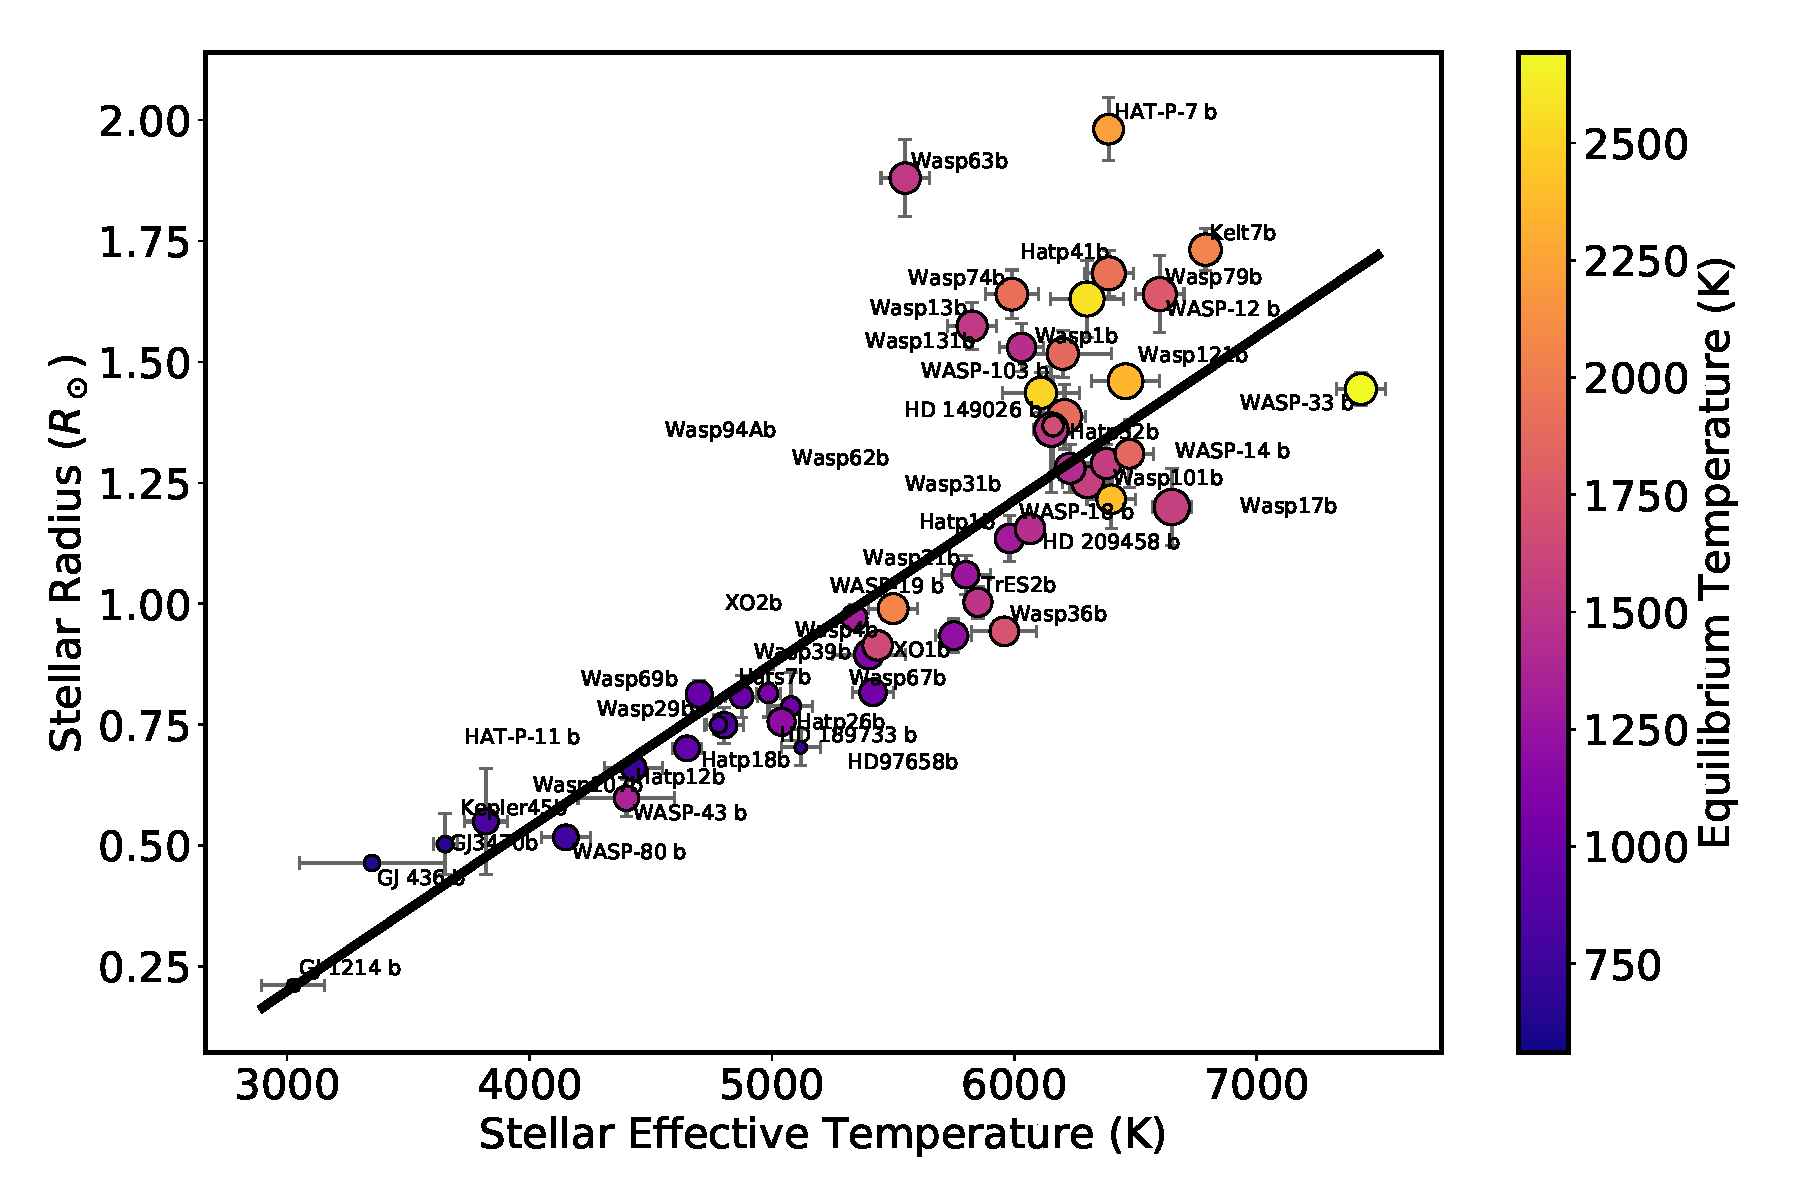
\includegraphics[width=\linewidth]{RsTs.pdf}
    \caption{Stellar Radius as a function of stellar effective temperature. Black line shows first order polynomial best fit used for creation of T-P grid (see Section \ref{P1:subsec:TPcreation}). Color of points shows the equilibrium temperature of the planets, size of points is scaled to the planet radius.}
    \label{P1:fig:RsTs}
\end{figure}

In our survey, most hot Jupiters populate a small range of close-in orbits, $a_{mean}$ = 0.037 $\pm$ 0.013 AU, while the parent stars span several spectral types, from early M stars to F stars. In fact, the stellar temperature varies from about 3000~K to 7000~K, while the radius also increases with earlier stellar types. Since for a planet at orbital distance ($a$) around a star with radius ($R_s$) and effective temperature ($T_{\rm eff}$), the equilibrium temperature of the planet ($T_{\rm eq}$) is proportional to $T_{\rm eff} (R_s/a)^{1/2}$. The stellar flux plays a bigger factor in determining the irradiation the planet received and its effective temperature. In this regard, we assume a fixed orbital distance for our model grid to isolate the effects of stellar irradiation. The mean value of the samples, 0.035 AU, is taken across the grid. In this setting, the effective temperature of the model planet is entirely determined by the stellar luminosity, and not by the orbital distance. We also note that the intrinsic temperature ($T_{\rm int}$) is negligible and thus the effective temperature ($T_{\rm eff}^4 = T_{\rm eq}^4 + T_{\rm int}^4$) is the same as the equilibrium temperature. Additionally, our assumed value of $T_{\rm int}$=150~K has little effect on our model temperature pressure profiles of the hot Jupiters.

The next step is to determine the size, hence the energy flux of the stars. For main-sequence stars which follow the mass--luminosity and mass-radius relations, we fit a power law relation between the radius and effective temperature, see Figure \ref{P1:fig:RsTs}. The power law fitting to our sample yields the following expression for the stellar radius: $R_S = m*T_{\rm eff} + b $ where $m$ and $b$ are 0.0003381 and -0.81495, respectively. Once the effective temperature and the radius of the star are known, there is enough information to specify the incident irradiation of the model atmospheres.

We then compute the T-P profiles for the given stellar irradiation using the analytical double-gray radiative equilibrium solutions in \citet{Heng2014} (Equation 126.).

The parameters used in this calculation are chosen to match numerical radiative transfer results, listed in Table \ref{P1:tab:TPparams}.
Similar to the prescriptions in  \citet{Guillot2010} and \citet{Parmentier2014}, the opacities do not have a pressure dependence.
We reiterate that this relation allows us to uniquely express the equilibrium temperature of a planet at a given orbital distance as a function of stellar temperature. Our stellar grid, with effective temperatures from 3250 to 7000~K, produces irradiated atmospheres of temperature from 446 to 2248 K, at 0.035 AU. To reach the temperatures of the ultra-hot jupiters we also run additional models with an orbital distance at 0.02 AU. The resulting temperature pressure profiles are shown in Figure \ref{P1:fig:TPgrid}.

The simple prescription allows us to explore the parameter space in a basic way and to focus on the correlation with stellar irradiation. Although the intrinsic temperature is held constant in our T-P profiles, the realistic interior can be potentially hotter. \citet{Tremblin2017} and \citet{Sainsbury-Martinez2019} have shown that circulation can transport entropy downward and leads to a hotter deep interior over time. \citet{Thorngren2019} suggested much higher $T_{\rm int}$ for observed hot Jupiters (with $T_{\rm eq}$ $\gtrsim$ 1300 K) than the 100K commonly assumed in GCMs. \citet{Fortney2020} also investigated the effects of heating from tidal dissipation for warm Jupiters (with $T_{\rm eq}$ $\gtrsim$ 1300 K) with simplified chemical timescale analysis. The upshot of the hotter interior is lowering the quenched [\ce{CH4}]/[\ce{CO}] ratio. In short, a hot deep interior changes the expectation for equilibrium chemistry in deep layers, hence the expectation from disequilibrium chemistry higher up. Since the equilibrium abundance of \ce{CH4} generally increases with depth (at least in our solar and 30x solar models), lowering vertical mixing also results in a lower [\ce{CH4}]/[\ce{CO}] ratio and can effectively be degenerate with a hotter interior. However, we find high vertical mixing matches the hot Jupiters better, even with the lower $T_{\rm int}$ of 150 K. Increasing the interior temperature will reduce \ce{CH4}, so even higher vertical mixing would be required to recover the same \ce{CH4} abundance for these planets. As for the cooler planets, the signature leading to our inference of low vertical mixing can also be explained by a hot interior if there is actually no \ce{CH4} in the deep hot atmosphere. However, the sources of internal heating and their exact interior temperature for these cool planets are rather uncertain (see \citet{Fortney2020} for a  detailed discussion).

In addition to this, our prescription for PT profiles is simplified compared to 1D radiative/convective models. Nevertheless, in this study, we are interested in the relative difference between two broad bandpasses (3.6 and 4.5~$\mu$m), and thus the prescription used for the TP profiles is less critical than for absolute measurements. The relative difference between 3.6 and 4.5~$\mu$m is globally similar for our prescription as compared to the 1D RC models. We aknowledge that the vertical mixing is likely to be affected by the choice of TPs, however testing this difference is beyond the scope of our current study.

Our simple model emphasizes the importance of the degeneracies between vertical mixing, interior temperature, and equilibrium chemistry, but is also a limit to the interpretation. A more detailed approach than the simple model we used is required to study the impact of the various processes on the observations with greater accuracy. However, such detailed study will also be limited by the unknown interior temperature. Therefore, we limit ourselves to a simple approach as a sophisticated analysis with more advanced temperature pressure profiles is beyond the scope of this paper.

\begin{table}[]
   \caption{Fixed parameters used in the double-grey radiative
equilibrium solution for creating temperature pressure profiles. For each TP profile we show the fixed irradiation temperature ($T_{\rm irr}$), intrinsic temperature ($T_{\rm int}$), longwave opacity ($\kappa_L$), shortwave opacity ($\kappa_S$), longwave scattering parameter ($\beta_{L}$) and the shortwave scattering parameter ($\beta_{S}$).}
   \centering
   \begin{tabular}{lllllll}
   \hline\hline
    $T_{\rm irr}$ & $T_{\rm int}$  & $\kappa_L$ & $\kappa_S$ &
$\beta_{L}$ & $\beta_{S}$ \\
   \hline
 631 & 150 & 0.02 & 0.00035 & 1 & 1 \\
 775 & 150 & 0.02 & 0.00068 & 1 & 1 \\
 919 & 150 & 0.02 & 0.001 & 1 & 1 \\
1069 & 150 & 0.02 & 0.0014 & 1 & 1 \\
1222 & 150 & 0.02 & 0.0017 & 1 & 1 \\
1379 & 150 & 0.02 & 0.0019 & 1 & 1 \\
1540 & 150 & 0.02 & 0.0022 & 1 & 1 \\
1706 & 150 & 0.02 & 0.0035 & 1 & 1 \\
1875 & 150 & 0.02 & 0.0038 & 1 & 1 \\
2049 & 150 & 0.02 & 0.004 & 1 & 1 \\
2227 & 150 & 0.02 & 0.0043 & 1 & 1 \\
2410 & 150 & 0.02 & 0.006 & 1 & 1 \\
2595 & 150 & 0.02 & 0.006 & 1 & 1 \\
2786 & 150 & 0.02 & 0.006 & 1 & 1 \\
2980 & 150 & 0.02 & 0.0061 & 1 & 1 \\
3179 & 150 & 0.02 & 0.0062 & 1 & 1 \\

   \hline
   \end{tabular}
   \label{P1:tab:TPparams}
\end{table}

\subsubsection{Grid of stellar spectra}

As the effective temperature of the star rises, the spectral energy distribution shifts to shorter wavelengths. We therefore adopted the stellar spectral grid from \citep{Rugheimer2013}, which ranges from 4250 to 7000 K and covers F0 to K7 spectral types. The models start with the synthetic ATLAS spectra \citep{Kurucz1979} and then we co-add the observed spectra from International Ultraviolet Explorer for UV (<= 300 nm). See \citep{Rugheimer2013} for the detailed stellar grid setup. Additionally, for late K and M stars ($T_{\rm eff}$ < 4250 K), we picked GJ 436 ($T_{\rm eff}$ = 3350 K) as our fiducial star. The high resolution spectrum of GJ436 is taken from the MUSCLES survey \citep{France2016}\footnote{http://cos.colorado.edu/~kevinf/muscles.html} and scaled for the stellar fluxes with effective temperatures of 3250~K, 3500~K, 3750~K, and 4000~K.

\subsubsection{Modeling the photo-chemical kinetics with VULCAN}
\label{P1:subsec:VULCAN}

We explore the effects of photolysis, atmospheric mixing, and metallicity by using a photochemical kinetics model, VULCAN \citep{Tsai2017}\footnote{https://github.com/exoclime/VULCAN}. The code solves the steady-state chemical compositions for a given temperature-pressure profile and has been benchmarked for hot Jupiters. In this work, we use the updated version that includes nitrogen chemistry and photochemistry (Tsai et al. in preparation). The chemical model with updated nitrogen chemistry and photochemistry has been tested on nitrogen dominated atmospheres for super-Earths \citep{Zilinskas2020}. The N-C-H-O network consists of about 600 thermal reactions (including forward and reverse) and 40 photodissociation reactions. We validate our updated model against the one-dimensional photochemical and thermochemical kinetics and diffusion model presented in \citet{Moses2011} for HD209458b, see Figure \ref{P1:fig:HD209}.

Vertical mixing is simulated through means of an eddy diffusion co-efficient ($K_{zz}$), which assumes that atmospheric motion resembles diffusion when convection and turbulence occur on much smaller scales than the magnitude of the pressure scale height. We vary the eddy diffusion coefficient to explore various strengths of vertical mixing, with constant values of 10$^8$, 10$^{10}$, and 10$^{12}$~\cmcms. The choice of the values is consistent with those extracted from GCM simulations \citep{Moses2011, Parmentier2013, Zhang2018c, Komacek2019}. Furthermore, the elemental abundance of the atmosphere is assigned to two different metallicities: 1x solar and 30x solar \citep{Lodders2009a}.




\subsubsection{Creating the transmission spectra with PLATON}
\label{P1:subsec:PLATON}

Finally, transmission spectra are then simulated using the open-source, transit-depth calculator and retrieval tool, PLATON \citep{Zhang2019}\footnote{https://platon.readthedocs.io/en/latest/intro.html}. The code has been modified to take non-equilibrium compositions from our calculation, including \ce{CH4}, \ce{CO}, \ce{CO2}, \ce{C2H2}, \ce{H2O}, \ce{O2}, \ce{OH}, \ce{C2H4}, \ce{C2H6}, \ce{H2CO}, \ce{HCN}, \ce{NH3}, \ce{NO}. The main opacities relevant for the wavelengths of \spitzerIRAC are displayed in Figure \ref{P1:fig:opacities}. We assume chemical equilibrium for the rest of the species in PLATON. The details of the forward model can be found in \citet{Zhang2019}. We neglect stellar limb darkening in these models and the synthetic transit depth is expressed as $(R_p/R_s)^2$.

\begin{figure}
    \centering
    \includegraphics[width=\linewidth]{opacities2.png}
    \caption{Opacities for a chemical equilibrium atmosphere at 600~K (left) and 1400~K (right) at 0.1 bar. Top panels show the abundance weighted opacities for a solar composition atmosphere and the bottom panels show the abundance weighted opacities for a 30x solar composition atmosphere. Carbon monoxide, water, methane and carbon dioxide (for 30x solar) are the dominant absorbing species at the two IRAC channels (3.6 and 4.5~$\mu$m).}
    \label{P1:fig:opacities}
\end{figure}


\subsubsection{Calculating the model \spitzerIRAC transit depths}

We integrate the simulated transmission spectra with \spitzerIRAC spectral response functions and weight with the stellar flux using the following equation:
\begin{equation}
\overline{\delta}_{\lambda} = \frac{\int_0^\infty  \delta(\lambda) \lambda R(\lambda) F_{s}(\lambda) d\lambda}{\int_0^\infty  \lambda R(\lambda) F_{s}(\lambda) d\lambda}
\end{equation}
where $R(\lambda)$ is the spectral response function at either 3.6~$\mu$m or 4.5~$\mu$m [e-/photon] \citep{Quijada2004} and $\delta(\lambda)$ is the transmission spectrum from PLATON and $F_{s}(\lambda)$ is the stellar flux. The output, $\overline{\delta}_{\lambda}$, is the weighted average transit depth that would be observed with \spitzerIRAC in either of the two bandpasses.

Figure \ref{P1:fig:ultimateplot} shows the interpolated grid of fiducial models (solar composition, cloud-free with equilibrium chemistry), we plot the normalized IRAC transit depth difference against the equilibrium temperature, and overplot the results from our transit survey. Figure \ref{P1:fig:tracks} shows the different tracks of the model grid that made up the shaded regions and Figure \ref{P1:fig:Kzzmodels} shows the different vertical mixing and metallicity interpolated grids with the data. For the cloudy grid, we simply assume a gray cloud opacity such that the spectra are flat and thus the transit depth difference would be zero, which is shown as a vertical line on Figures \ref{P1:fig:ultimateplot} and \ref{P1:fig:Kzzmodels}.

\begin{figure}[ht]
    \centering
    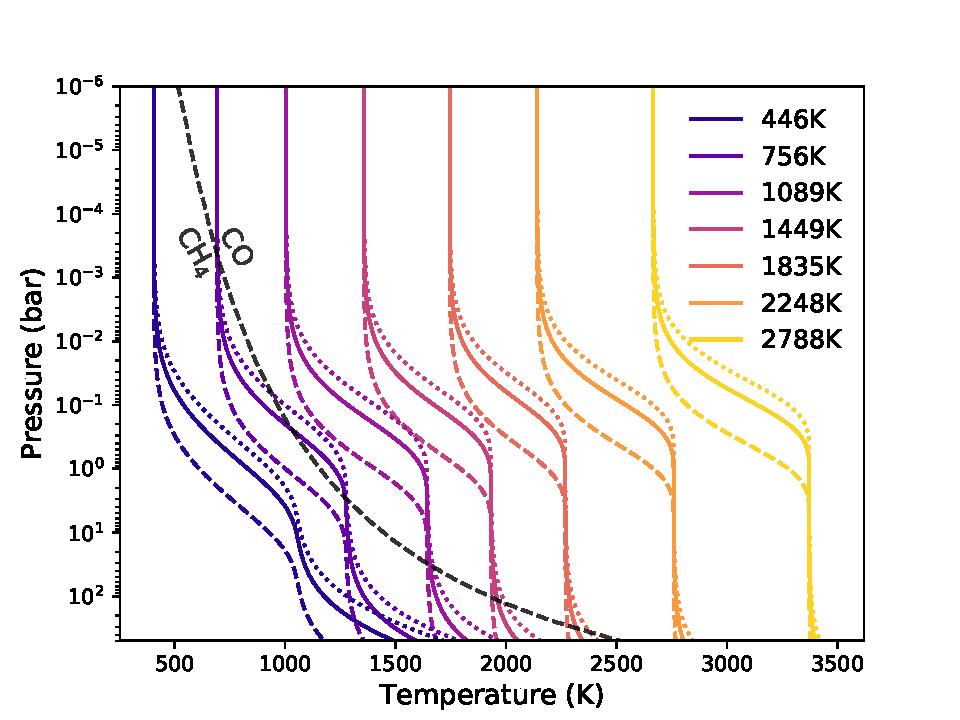
\includegraphics[width=\linewidth]{TPgrid2.pdf}
    \caption{Analytical Temperature-Pressure profiles for grid of models spanning equilibrium temperatures $\sim$400-2800~K, showing every $\sim$400~K. For each temperature we show three profiles where the surface gravity is varied: dotted, solid and dashed lines represent 500, 1000 and 5000~\cmss~respectively. Grey dashed line represents the gas transition between \ce{CH4} and \ce{CO} dominated atmospheres when chemical equilibrium is assumed.}
    \label{P1:fig:TPgrid}
\end{figure}


\section{Results}
\label{P1:sec:Results}

\subsection{Measured transit depths and their ratios}

\subsubsection{Results of measured transit depths}

\longtab{

\setlength{\tabcolsep}{3pt}

\begin{longtable}[h]{lllllll}

\caption{\label{P1:tab:results} Results from the MCMC analysis, we show the semi-major axis (a/R*), the inclination (degrees), the percentage transit depth $(R_p/R_s)^2$, the corresponding impact parameter (b) and the mid-transit time in BJD\_UTC. Values for the semi-major axis and the inclination are from the initial MCMC fits and then these are fixed with gaussian priors for a second MCMC run where the final values for the transit depths are determined.}\\

\hline\hline
Planet & $\lambda$  & a/R* & inc  & depth  &     b & T0 \\
& $(\mu m)$ & & degrees & $(R_p/R_s)^2$ & &  BJD\_UTC \\
& & & & (\%) & & \\

\hline
\endfirsthead
\caption{continued.} \\
\hline\hline
Planet & $\lambda$  & a/R* & inc  & depth  &     b & T0 \\
& $(\mu m)$ & & degrees & $(R_p/R_s)^2$ & & BJD\_UTC \\
& & & & (\%) & & \\

\hline
\endhead
\hline
\endfoot

HAT-P-32 b   &               3.6 &   ${6.13}^{+0.02}_{-0.02}$ &  ${89.5}^{+0.3}_{-0.5}$ &  ${2.15}^{+0.01}_{-0.01}$ &    ${0.05}^{+2.06}_{-2.90}$ &  ${2456250.103520}^{+0.000112}_{-0.000120}$ \\
HAT-P-32 b   &               4.5 &   ${6.13}^{+0.02}_{-0.04}$ &  ${89.4}^{+0.4}_{-0.6}$ &  ${2.21}^{+0.02}_{-0.02}$ &    ${0.06}^{+2.62}_{-3.95}$ &  ${2456370.504208}^{+0.000154}_{-0.000152}$ \\
XO-1 b      &               3.6 &  ${11.46}^{+0.05}_{-0.11}$ &  ${89.5}^{+0.3}_{-0.4}$ &  ${1.67}^{+0.01}_{-0.01}$ &    ${0.09}^{+3.56}_{-4.43}$ &  ${2456426.076095}^{+0.000115}_{-0.000120}$ \\
XO-1 b      &               4.5 &  ${11.24}^{+0.20}_{-0.23}$ &  ${88.8}^{+0.5}_{-0.4}$ &  ${1.72}^{+0.01}_{-0.01}$ &    ${0.24}^{+5.40}_{-4.49}$ &  ${2456437.900819}^{+0.000158}_{-0.000157}$ \\
HAT-P-1 b    &               3.6 &   ${9.91}^{+0.13}_{-0.13}$ &  ${85.7}^{+0.1}_{-0.1}$ &  ${1.40}^{+0.01}_{-0.01}$ &    ${0.74}^{+0.99}_{-0.99}$ &  ${2456547.478364}^{+0.000156}_{-0.000150}$ \\
HAT-P-1 b    &               4.5 &  ${10.07}^{+0.16}_{-0.15}$ &  ${85.8}^{+0.1}_{-0.1}$ &  ${1.39}^{+0.01}_{-0.01}$ &    ${0.73}^{+1.25}_{-1.17}$ &  ${2456556.409109}^{+0.000187}_{-0.000190}$ \\
WASP-17 b   &               3.6 &   ${7.16}^{+0.14}_{-0.16}$ &  ${88.1}^{+0.8}_{-0.7}$ &  ${1.52}^{+0.01}_{-0.01}$ &    ${0.24}^{+6.05}_{-4.97}$ &  ${2456423.188874}^{+0.000233}_{-0.000221}$ \\
WASP-17 b   &               4.5 &   ${7.24}^{+0.09}_{-0.15}$ &  ${88.6}^{+0.8}_{-0.8}$ &  ${1.57}^{+0.02}_{-0.02}$ &    ${0.17}^{+6.13}_{-5.89}$ &  ${2456426.923243}^{+0.000288}_{-0.000285}$ \\
WASP-39 b   &               3.6 &  ${10.47}^{+0.19}_{-0.17}$ &  ${87.0}^{+0.2}_{-0.2}$ &  ${2.15}^{+0.02}_{-0.02}$ &    ${0.56}^{+1.83}_{-1.68}$ &  ${2456401.396438}^{+0.000159}_{-0.000176}$ \\
WASP-39 b   &               4.5 &  ${11.38}^{+0.28}_{-0.25}$ &  ${87.7}^{+0.3}_{-0.2}$ &  ${2.16}^{+0.02}_{-0.02}$ &    ${0.45}^{+3.14}_{-2.66}$ &  ${2456575.774315}^{+0.000200}_{-0.000194}$ \\
HAT-P-12 b   &               3.6 &  ${11.23}^{+0.26}_{-0.26}$ &  ${88.0}^{+0.3}_{-0.3}$ &  ${1.89}^{+0.01}_{-0.01}$ &    ${0.39}^{+3.64}_{-3.30}$ &  ${2456359.882148}^{+0.000131}_{-0.000138}$ \\
HAT-P-12 b   &               4.5 &  ${10.90}^{+0.35}_{-0.30}$ &  ${87.8}^{+0.4}_{-0.3}$ &  ${1.93}^{+0.03}_{-0.03}$ &    ${0.41}^{+4.47}_{-3.60}$ &  ${2456363.095398}^{+0.000197}_{-0.000187}$ \\
HAT-P-18 b   &               3.6 &  ${15.28}^{+0.47}_{-0.41}$ &  ${88.5}^{+0.3}_{-0.3}$ &  ${1.77}^{+0.02}_{-0.02}$ &    ${0.41}^{+5.19}_{-4.07}$ &  ${2456461.067141}^{+0.000195}_{-0.000197}$ \\
HAT-P-18 b   &               4.5 &  ${15.48}^{+0.45}_{-0.44}$ &  ${88.5}^{+0.3}_{-0.3}$ &  ${1.93}^{+0.02}_{-0.02}$ &    ${0.41}^{+5.07}_{-4.47}$ &  ${2456483.099518}^{+0.000215}_{-0.000215}$ \\
TrES-2 b    &               3.6 &   ${7.96}^{+0.16}_{-0.15}$ &  ${83.9}^{+0.2}_{-0.2}$ &  ${1.37}^{+0.02}_{-0.02}$ &    ${0.84}^{+1.33}_{-1.34}$ &  ${2456252.834601}^{+0.000203}_{-0.000196}$ \\
TrES-2 b    &               4.5 &   ${8.20}^{+0.25}_{-0.23}$ &  ${84.2}^{+0.3}_{-0.2}$ &  ${1.40}^{+0.02}_{-0.02}$ &    ${0.83}^{+2.09}_{-1.92}$ &  ${2456257.775215}^{+0.000268}_{-0.000267}$ \\
WASP-4 b    &               3.6 &   ${5.58}^{+0.03}_{-0.04}$ &  ${89.3}^{+0.5}_{-0.7}$ &  ${2.28}^{+0.02}_{-0.02}$ &    ${0.07}^{+2.71}_{-4.14}$ &  ${2456288.955465}^{+0.000137}_{-0.000142}$ \\
WASP-4 b    &               4.5 &   ${5.46}^{+0.05}_{-0.11}$ &  ${88.7}^{+0.9}_{-1.3}$ &  ${2.34}^{+0.03}_{-0.03}$ &    ${0.12}^{+4.80}_{-7.20}$ &  ${2456292.969500}^{+0.000208}_{-0.000212}$ \\
XO-2 b      &               3.6 &   ${8.17}^{+0.09}_{-0.17}$ &  ${88.9}^{+0.7}_{-0.8}$ &  ${1.07}^{+0.01}_{-0.01}$ &    ${0.15}^{+5.81}_{-6.13}$ &  ${2456295.370617}^{+0.000139}_{-0.000140}$ \\
XO-2 b      &               4.5 &   ${7.77}^{+0.22}_{-0.22}$ &  ${87.6}^{+0.7}_{-0.6}$ &  ${1.07}^{+0.01}_{-0.01}$ &    ${0.33}^{+5.43}_{-4.50}$ &  ${2456292.754728}^{+0.000198}_{-0.000191}$ \\
GJ3470 b   &               3.6 &  ${14.63}^{+0.52}_{-0.50}$ &  ${88.4}^{+0.3}_{-0.3}$ &  ${0.57}^{+0.01}_{-0.01}$ &    ${0.42}^{+4.13}_{-3.73}$ &  ${2456284.001794}^{+0.000118}_{-0.000115}$ \\
GJ3470 b   &               4.5 &  ${14.41}^{+0.65}_{-0.54}$ &  ${88.4}^{+0.4}_{-0.3}$ &  ${0.61}^{+0.01}_{-0.01}$ &    ${0.41}^{+5.23}_{-4.09}$ &  ${2456294.011801}^{+0.000151}_{-0.000150}$ \\
WASP-21 b   &               3.6 &   ${9.55}^{+0.30}_{-0.28}$ &  ${87.1}^{+0.4}_{-0.4}$ &  ${1.08}^{+0.01}_{-0.01}$ &    ${0.49}^{+3.75}_{-3.34}$ &  ${2456532.561048}^{+0.000261}_{-0.000260}$ \\
WASP-21 b   &               4.5 &   ${9.61}^{+0.40}_{-0.34}$ &  ${87.1}^{+0.5}_{-0.4}$ &  ${1.14}^{+0.02}_{-0.02}$ &    ${0.48}^{+5.28}_{-4.23}$ &  ${2456536.882998}^{+0.000308}_{-0.000322}$ \\
WASP-31 b   &               3.6 &   ${8.06}^{+0.20}_{-0.18}$ &  ${84.5}^{+0.2}_{-0.2}$ &  ${1.54}^{+0.02}_{-0.02}$ &    ${0.77}^{+1.81}_{-1.66}$ &  ${2456360.907660}^{+0.000317}_{-0.000328}$ \\
WASP-31 b   &               4.5 &   ${8.86}^{+0.34}_{-0.32}$ &  ${85.2}^{+0.3}_{-0.3}$ &  ${1.50}^{+0.03}_{-0.03}$ &    ${0.74}^{+2.86}_{-2.77}$ &  ${2456371.125690}^{+0.000407}_{-0.000412}$ \\
WASP-1 b    &               3.6 &   ${5.72}^{+0.03}_{-0.05}$ &  ${89.3}^{+0.5}_{-0.8}$ &  ${1.07}^{+0.01}_{-0.01}$ &    ${0.07}^{+2.91}_{-4.60}$ &  ${2456361.902274}^{+0.000263}_{-0.000250}$ \\
WASP-1 b    &               4.5 &   ${5.41}^{+0.17}_{-0.20}$ &  ${86.5}^{+1.2}_{-1.1}$ &  ${1.09}^{+0.02}_{-0.02}$ &    ${0.33}^{+6.58}_{-6.12}$ &  ${2456371.982150}^{+0.000354}_{-0.000364}$ \\
HAT-P-26 b   &               3.6 &  ${13.22}^{+0.75}_{-0.94}$ &  ${88.3}^{+0.8}_{-0.7}$ &  ${0.53}^{+0.01}_{-0.01}$ &   ${0.39}^{+10.08}_{-9.85}$ &  ${2456545.361384}^{+0.000296}_{-0.000288}$ \\
HAT-P-26 b   &               4.5 &  ${13.92}^{+0.16}_{-0.32}$ &  ${89.5}^{+0.3}_{-0.6}$ &  ${0.55}^{+0.01}_{-0.01}$ &    ${0.11}^{+4.33}_{-8.72}$ &  ${2456405.622835}^{+0.000356}_{-0.000364}$ \\
WASP-107 b  &               3.6 &  ${18.19}^{+0.03}_{-0.04}$ &  ${89.9}^{+0.1}_{-0.1}$ &  ${1.96}^{+0.01}_{-0.01}$ &    ${0.04}^{+1.45}_{-2.26}$ &  ${2457876.124941}^{+0.000060}_{-0.000064}$ \\
WASP-107 b  &               4.5 &  ${18.09}^{+0.05}_{-0.09}$ &  ${89.8}^{+0.1}_{-0.2}$ &  ${2.06}^{+0.01}_{-0.01}$ &    ${0.06}^{+2.54}_{-3.09}$ &  ${2457870.403743}^{+0.000081}_{-0.000077}$ \\
WASP-13 b   &               3.6 &   ${7.64}^{+0.20}_{-0.19}$ &  ${85.6}^{+0.4}_{-0.3}$ &  ${0.86}^{+0.01}_{-0.01}$ &    ${0.58}^{+2.70}_{-2.50}$ &  ${2456480.940869}^{+0.000231}_{-0.000246}$ \\
WASP-13 b   &               4.5 &   ${7.78}^{+0.27}_{-0.23}$ &  ${85.7}^{+0.4}_{-0.4}$ &  ${0.87}^{+0.01}_{-0.01}$ &    ${0.59}^{+3.43}_{-2.85}$ &  ${2456315.526437}^{+0.000293}_{-0.000303}$ \\
WASP-121 b  &               3.6 &   ${3.84}^{+0.02}_{-0.03}$ &  ${88.9}^{+0.8}_{-1.1}$ &  ${1.47}^{+0.01}_{-0.01}$ &    ${0.07}^{+2.95}_{-4.10}$ &  ${2457906.807311}^{+0.000148}_{-0.000144}$ \\
WASP-121 b  &               4.5 &   ${3.82}^{+0.02}_{-0.03}$ &  ${89.0}^{+0.8}_{-1.3}$ &  ${1.49}^{+0.01}_{-0.01}$ &    ${0.07}^{+3.02}_{-4.80}$ &  ${2457910.632374}^{+0.000183}_{-0.000171}$ \\
WASP-69 b   &               3.6 &  ${12.26}^{+0.09}_{-0.08}$ &  ${86.8}^{+0.0}_{-0.0}$ &  ${1.60}^{+0.00}_{-0.00}$ &    ${0.68}^{+0.60}_{-0.58}$ &  ${2457992.354188}^{+0.000053}_{-0.000054}$ \\
WASP-69 b   &               4.5 &  ${12.30}^{+0.11}_{-0.10}$ &  ${86.8}^{+0.1}_{-0.1}$ &  ${1.67}^{+0.01}_{-0.01}$ &    ${0.68}^{+0.77}_{-0.71}$ &  ${2457996.222243}^{+0.000066}_{-0.000069}$ \\
WASP-67 b   &               3.6 &  ${13.50}^{+0.39}_{-0.33}$ &  ${86.2}^{+0.2}_{-0.2}$ &  ${1.97}^{+0.03}_{-0.03}$ &    ${0.91}^{+2.28}_{-2.72}$ &  ${2457776.271136}^{+0.000219}_{-0.000220}$ \\
WASP-67 b   &               4.5 &  ${13.90}^{+0.31}_{-0.39}$ &  ${86.3}^{+0.1}_{-0.1}$ &  ${1.92}^{+0.03}_{-0.03}$ &    ${0.89}^{+1.84}_{-1.93}$ &  ${2457979.305753}^{+0.000282}_{-0.000276}$ \\
HATS-7 b    &               3.6 &  ${11.09}^{+0.62}_{-1.07}$ &  ${88.2}^{+1.0}_{-1.3}$ &  ${0.38}^{+0.02}_{-0.02}$ &  ${0.35}^{+11.03}_{-14.14}$ &  ${2457694.120917}^{+0.000590}_{-0.000538}$ \\
HATS-7 b    &               4.5 &  ${10.80}^{+0.48}_{-0.91}$ &  ${88.4}^{+1.1}_{-1.2}$ &  ${0.40}^{+0.03}_{-0.03}$ &  ${0.30}^{+12.05}_{-13.12}$ &  ${2457697.305788}^{+0.000797}_{-0.000795}$ \\
WASP-29 b   &               3.6 &  ${12.58}^{+0.05}_{-0.11}$ &  ${89.7}^{+0.2}_{-0.4}$ &  ${0.95}^{+0.01}_{-0.01}$ &    ${0.07}^{+2.95}_{-4.91}$ &  ${2457807.234478}^{+0.000115}_{-0.000120}$ \\
WASP-29 b   &               4.5 &  ${12.53}^{+0.05}_{-0.08}$ &  ${89.7}^{+0.2}_{-0.3}$ &  ${0.93}^{+0.01}_{-0.01}$ &    ${0.06}^{+2.59}_{-4.13}$ &  ${2457826.848225}^{+0.000150}_{-0.000149}$ \\
HAT-P-41 b   &               3.6 &   ${5.53}^{+0.03}_{-0.06}$ &  ${89.0}^{+0.7}_{-0.9}$ &  ${1.00}^{+0.01}_{-0.01}$ &    ${0.10}^{+3.76}_{-4.92}$ &  ${2457772.203860}^{+0.000220}_{-0.000217}$ \\
HAT-P-41 b   &               4.5 &   ${5.55}^{+0.03}_{-0.04}$ &  ${89.3}^{+0.5}_{-0.8}$ &  ${1.09}^{+0.01}_{-0.01}$ &    ${0.07}^{+2.78}_{-4.43}$ &  ${2457788.367795}^{+0.000274}_{-0.000263}$ \\
WASP-101 b  &               3.6 &   ${8.60}^{+0.17}_{-0.16}$ &  ${85.2}^{+0.2}_{-0.2}$ &  ${1.18}^{+0.01}_{-0.01}$ &    ${0.73}^{+1.55}_{-1.54}$ &  ${2457760.332526}^{+0.000170}_{-0.000175}$ \\
WASP-101 b  &               4.5 &   ${8.51}^{+0.19}_{-0.18}$ &  ${85.0}^{+0.2}_{-0.2}$ &  ${1.14}^{+0.01}_{-0.01}$ &    ${0.74}^{+1.72}_{-1.64}$ &  ${2457771.089626}^{+0.000225}_{-0.000227}$ \\
WASP-131 b  &               3.6 &   ${8.34}^{+0.20}_{-0.19}$ &  ${85.0}^{+0.2}_{-0.2}$ &  ${0.61}^{+0.01}_{-0.01}$ &    ${0.73}^{+1.88}_{-1.80}$ &  ${2457696.837080}^{+0.000253}_{-0.000256}$ \\
WASP-131 b  &               4.5 &   ${8.41}^{+0.28}_{-0.26}$ &  ${85.0}^{+0.3}_{-0.3}$ &  ${0.61}^{+0.01}_{-0.01}$ &    ${0.73}^{+2.63}_{-2.53}$ &  ${2457909.718452}^{+0.000336}_{-0.000332}$ \\
WASP-36 b   &               3.6 &   ${6.06}^{+0.25}_{-0.22}$ &  ${83.7}^{+0.6}_{-0.5}$ &  ${1.78}^{+0.03}_{-0.03}$ &    ${0.67}^{+3.75}_{-3.19}$ &  ${2457805.166629}^{+0.000262}_{-0.000262}$ \\
WASP-36 b   &               4.5 &   ${6.19}^{+0.44}_{-0.39}$ &  ${84.4}^{+1.1}_{-1.0}$ &  ${1.82}^{+0.03}_{-0.03}$ &    ${0.60}^{+6.70}_{-6.13}$ &  ${2457975.813843}^{+0.000346}_{-0.000353}$ \\
WASP-63 b   &               3.6 &   ${6.26}^{+0.23}_{-0.21}$ &  ${86.6}^{+1.0}_{-0.8}$ &  ${0.61}^{+0.01}_{-0.01}$ &    ${0.37}^{+6.38}_{-5.07}$ &  ${2457865.520635}^{+0.000353}_{-0.000330}$ \\
WASP-63 b   &               4.5 &   ${6.52}^{+0.16}_{-0.21}$ &  ${87.7}^{+1.1}_{-1.0}$ &  ${0.55}^{+0.01}_{-0.01}$ &    ${0.26}^{+7.01}_{-6.45}$ &  ${2457922.436423}^{+0.000470}_{-0.000461}$ \\
WASP-79 b   &               3.6 &   ${7.31}^{+0.15}_{-0.14}$ &  ${85.9}^{+0.3}_{-0.3}$ &  ${1.20}^{+0.01}_{-0.01}$ &    ${0.52}^{+2.36}_{-2.05}$ &  ${2457713.374126}^{+0.000167}_{-0.000167}$ \\
WASP-79 b   &               4.5 &   ${7.12}^{+0.15}_{-0.14}$ &  ${85.6}^{+0.3}_{-0.3}$ &  ${1.17}^{+0.01}_{-0.01}$ &    ${0.55}^{+2.29}_{-2.02}$ &  ${2457720.699409}^{+0.000215}_{-0.000213}$ \\
WASP-94 Ab  &               3.6 &   ${7.34}^{+0.02}_{-0.04}$ &  ${89.5}^{+0.3}_{-0.5}$ &  ${1.12}^{+0.01}_{-0.01}$ &    ${0.06}^{+2.43}_{-3.56}$ &  ${2457795.021530}^{+0.000147}_{-0.000147}$ \\
WASP-94 Ab  &               4.5 &   ${7.34}^{+0.02}_{-0.04}$ &  ${89.5}^{+0.4}_{-0.5}$ &  ${1.13}^{+0.01}_{-0.01}$ &    ${0.07}^{+2.62}_{-3.61}$ &  ${2457972.780291}^{+0.000187}_{-0.000180}$ \\
WASP-74 b   &               3.6 &   ${4.75}^{+0.08}_{-0.07}$ &  ${79.7}^{+0.3}_{-0.2}$ &  ${0.87}^{+0.01}_{-0.01}$ &    ${0.85}^{+1.17}_{-1.01}$ &  ${2457768.164558}^{+0.000178}_{-0.000176}$ \\
WASP-74 b   &               4.5 &   ${5.13}^{+0.11}_{-0.10}$ &  ${80.8}^{+0.3}_{-0.3}$ &  ${0.86}^{+0.01}_{-0.01}$ &    ${0.82}^{+1.44}_{-1.42}$ &  ${2457770.304101}^{+0.000228}_{-0.000230}$ \\
WASP-62 b   &               3.6 &   ${9.47}^{+0.16}_{-0.16}$ &  ${88.2}^{+0.4}_{-0.3}$ &  ${1.29}^{+0.01}_{-0.01}$ &    ${0.30}^{+3.57}_{-3.02}$ &  ${2457717.229937}^{+0.000138}_{-0.000138}$ \\
WASP-62 b   &               4.5 &   ${9.32}^{+0.20}_{-0.18}$ &  ${87.9}^{+0.4}_{-0.3}$ &  ${1.20}^{+0.01}_{-0.01}$ &    ${0.35}^{+3.88}_{-3.05}$ &  ${2457730.466206}^{+0.000165}_{-0.000167}$ \\
Kepler-45 b &               3.6 &      - &   - &  ${3.37}^{+0.13}_{-0.13}$ &       - &  - \\
Kepler-45 b &               4.5 &      - &   - &  ${3.50}^{+0.14}_{-0.14}$ &       - &  - \\
\end{longtable}
}

\begin{figure}
    \centering
    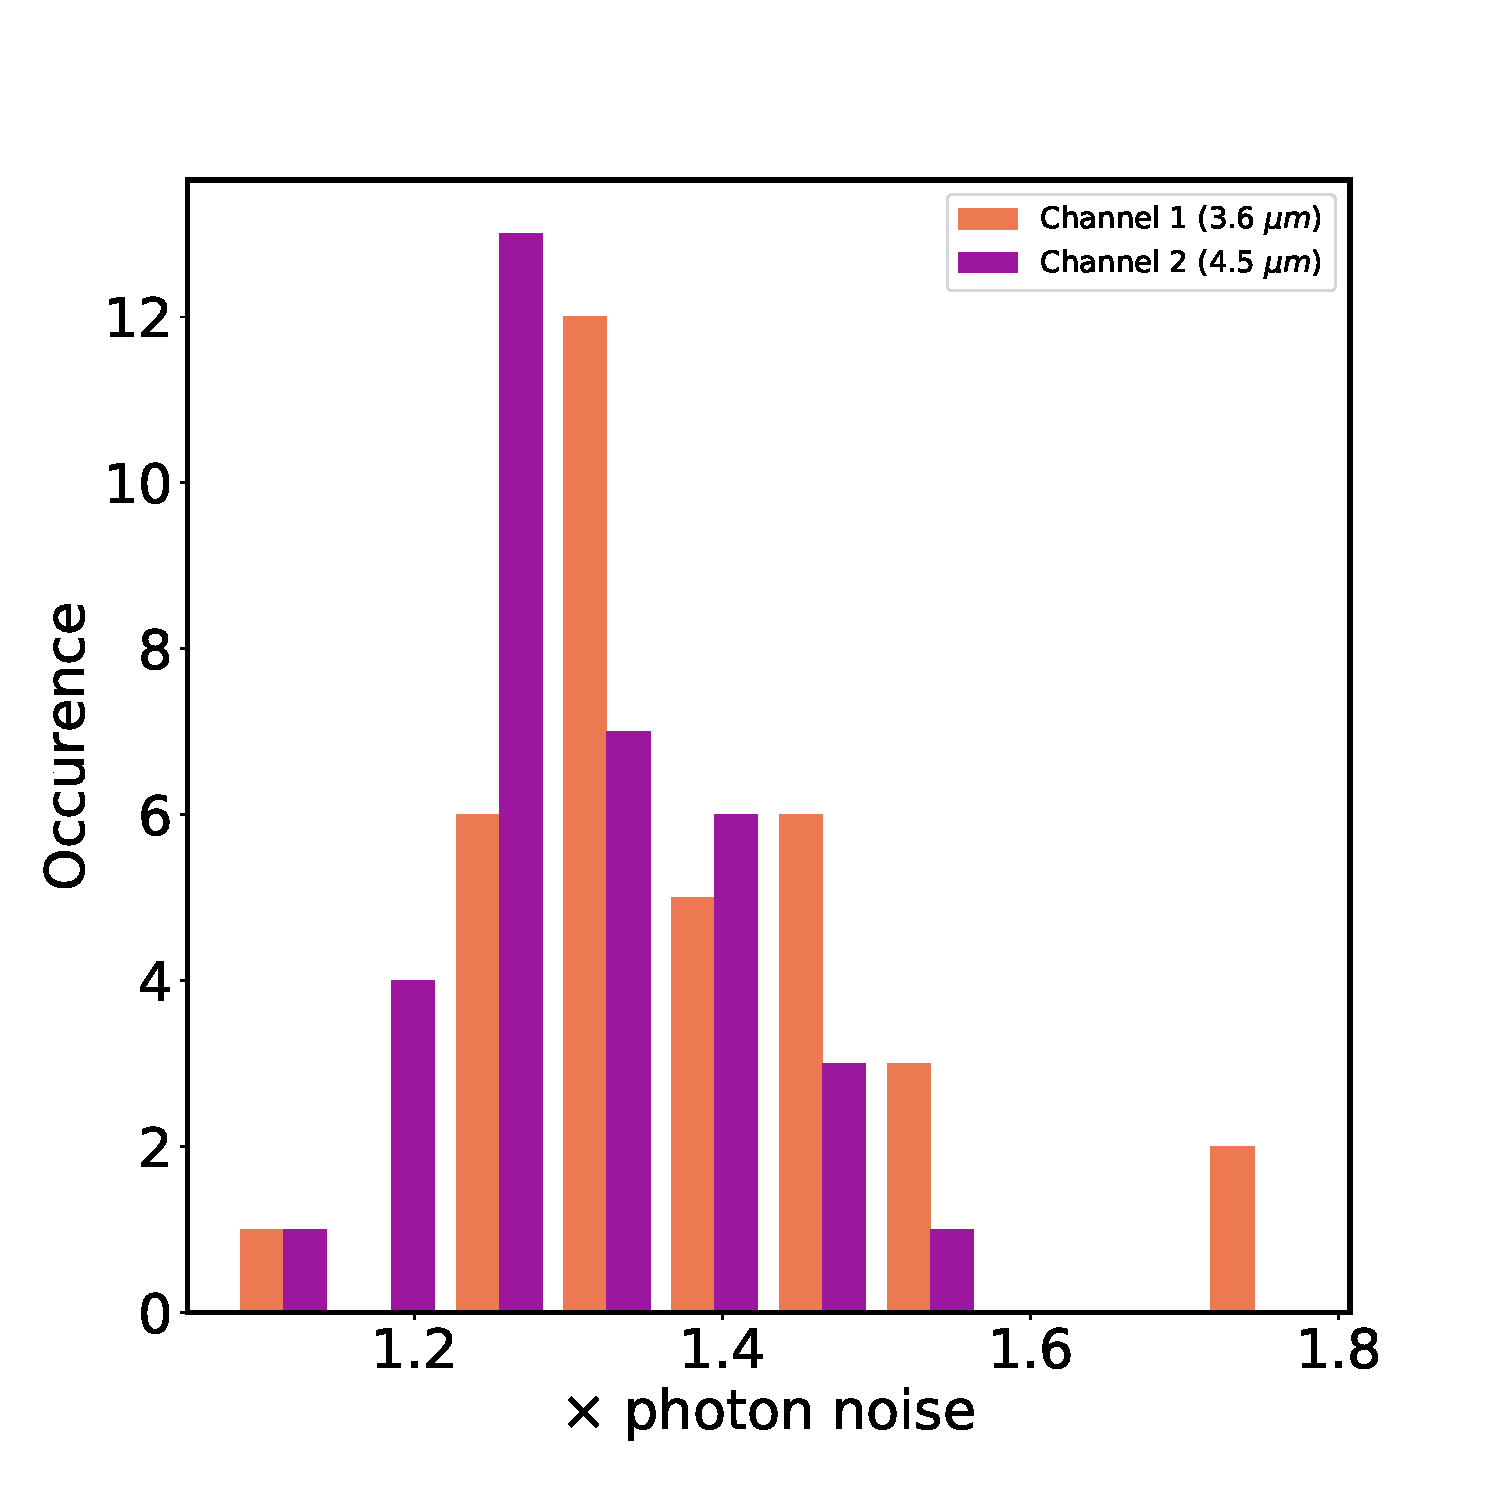
\includegraphics[width = \linewidth]{photonnoisehist.pdf}
    \caption{Histogram showing the percentage above photon noise for each of the individual lightcurves. Channel 1 (3.6~$\mu$m) is displayed in orange and channel 2 (4.5~$\mu$m) in purple.}
    \label{P1:fig:photonnoise}
\end{figure}

Table \ref{P1:tab:results} summarizes the results of the MCMC analysis of the lightcurves, and it lists the final values and uncertainties for the transit depths, mid transit times and impact parameters from the final fits as well as the inclination and semi-major axis obtained from the first fits. We checked that the initial fits of the semi-major axis and the inclination are in agreement with the literature values before fixing them with Gaussian priors for the second fit. The survey as a whole was in statistical agreement with the literature values within $<1\sigma$.

We also show the raw photometry with the best fit model for each visit in Appendix \ref{P1:app:piperes}, and we show the corresponding RMS vs binsize plots in Appendix \ref{P1:app:piperes}. Figure \ref{P1:fig:normlc1} shows the reduced, normalized and systematic corrected transit lightcurves for all planets in our sample for both channel 1 and channel 2 with the best fit model resulting from the MCMC. We calculate the residuals, the $\chi^2$ and the RMS of the residuals as sanity checks for each lightcurve (Table \ref{P1:tab:tests}).

As mentioned in Section \ref{P1:subsec:fitting}, before performing a complete MCMC analysis, we first check the fraction above photon noise and scale up the errors accordingly. Figure \ref{P1:fig:photonnoise} displays a histogram of the fraction above photon noise for all analyzed lightcurves. The histograms have a median of 1.36 and 1.27 times photon noise for 3.6~$\mu$m and 4.5~$\mu$m respectively, which is typical for what has been achieved with \spitzer in the past \citep{Ingalls2016}.

\subsubsection{Comparison to literature}

Several of the planets from our survey have had their \spitzer lightcurves previously analyzed \citet[e.g.,][]{Sing2016, Garhart2020}. We compare our results with those from \citet{Sing2016} and \citet{Garhart2020}. Our measured transits are consistent within 3-$\sigma$with those from the literature apart from a couple of outliers described below. Two of the largest outliers are the channel 2 transit depth of KELT-7b and the channel 1 transit depth of WASP-62b, both analyzed in \citet{Garhart2020} with PLD. We interpret the differences as due to the brightness of the host stars, and more specifically as due to the number of pixels selected for the pixel level decorrelation. These stars are bright and therefore 12 pixels are selected to model the systematics in \citet{Garhart2020} whereas we use 9 pixels uniformly for the entire survey. We emphasize that these differences do not affect the general conclusion of the paper.

\subsubsection{Transit depth ratio}
\label{P1:subsec:transit}

We combine our results with transit measurements from the literature, which results in a survey of transit depths at 3.6 and 4.5~$\mu$m for 49 planets spanning a large range of equilibrium temperatures. We now compare all targets in our survey in a statistical manner. To do this, we opt to use a metric that is as free as possible from any assumptions - the normalized difference of the transit depths:

\begin{equation}
     \bar{\Delta}_{tr} = \frac{(\delta_{ch2} - \delta_{ch1})}{\delta_{ch1}}
\end{equation}

With this calculation, we tested for correlations with a number of other parameters:  stellar parameters (Teff, logg, Fe/H, $R_s$), orbital parameters (semi-major axis (AU), eccentricity, inclination) and planetary parameters ($T_{\rm eq}$, logg, $R_p$, $M_p$, scale height). We looked for correlations between using two statistical methods. First, we calculated the Pearson correlation coefficient (r) and its associated chance probability (p). Then, we fit a straight line using an orthogonal distance regression (ODR) to account for the errors on both the abscissa and ordinate values \citet{Boggs1989} and look at the resulting residual variance of the fits.

\subsubsection{Searching for trends in the difference of transit depths}

We analyse our \spitzer survey by looking at the normalized difference in the transit depths. Our normalized transit depth difference metric has the benefit that it does not include any additional assumptions on the composition of the atmosphere.  Several studies look at the number of scale heights crossed at different wavelengths, including the strength of the water feature in the HST/ WFC3 bandpass \citep[e.g.,][]{Sing2016}. Including the scale height requires assuming the mean molecular weight, which includes errors from the surface gravity and equilibrium temperature. Furthermore, our metric is also independent of the stellar radius - unlike the difference in transit depths ($\delta_{ch2} - \delta_{ch1}$). Ultimately, this metric is a proxy for the ratio of the optical depths at these two wavelengths. We expect that the strength and magnitude of this metric can be used to test how the dominant expected atmospheric opacities change with the equilibrium temperature of the planets, see Section \ref{P1:subsec:Chemistry}.

\begin{table}
    \caption{Correlations between parameters and the transit depth ratio. We show the Pearson correlation coefficient ($r$), the associated chance probability ($p$) and the residual variance from an ODR linear fit to the data. }
    \label{P1:tab:pearson}
    \centering
\begin{tabular}{lccc}
%\centering
\hline\hline
Parameter &  $r$ &  $p$ &  Res Var \\
\hline
$T_{\rm eq}$ (a=0)      &                            -0.35 &            0.01 &               7.23 \\
$T_{\rm eff}$           &                            -0.34 &            0.02 &               7.14 \\
Stellar log(g)          &                             0.13 &            0.36 &               6.98 \\
$[$Fe/H$]$  &                            -0.21 &            0.15 &               4.48 \\
$R_p$              &                            -0.26 &            0.07 &               8.11 \\
Inclination            &                             0.20 &            0.18 &               7.03 \\
a (AU)         &                             0.07 &            0.63 &               8.46 \\
Planetary log(g)          &                             0.01 &            0.92 &               8.47 \\
$M_p$ ($M_J$)      &                             0.09 &            0.56 &               8.78 \\
H (km)             &                            -0.17 &            0.25 &               8.50 \\
$R_s$ ($R_{\odot}$)      &                            -0.40 &            0.00 &               7.06 \\
Radius Anomaly &                            -0.25 &            0.14 &               6.86 \\
\hline
\end{tabular}
\end{table}


We search for any correlations that could be present between the calculated normalized transit depth difference and the physical parameters of the planetary systems that we are exploring. Table \ref{P1:tab:pearson} summarizes the correlations for each of the parameters. The three parameters with the strongest Pearson correlation coefficients and the lowest chance probabilities are $T_{\rm eq}$, $T_{\rm eff}$ and $R_s$. Both $T_{\rm eff}$ and $R_s$ are incidentally included in the calculation of the equilibrium temperature, $T_{\rm eq}$ (in our case with zero albedo and full redistribution). We also observe that the weakest correlations are with the planetary mass, planetary radius, and semi-major axis. This is not surprising since our sample is highly biased towards hot Jupiters with a relatively small range of radii and masses, and with similarly close-in orbits. This means that the span of these parameters is small and therefore the uncertainties will be large and the correlations will not be obvious.

\subsubsection{Transit depth versus equilibrium temperature}
\label{P1:subsec:TDvsTeq}

\begin{sidewaysfigure}
    \centering
    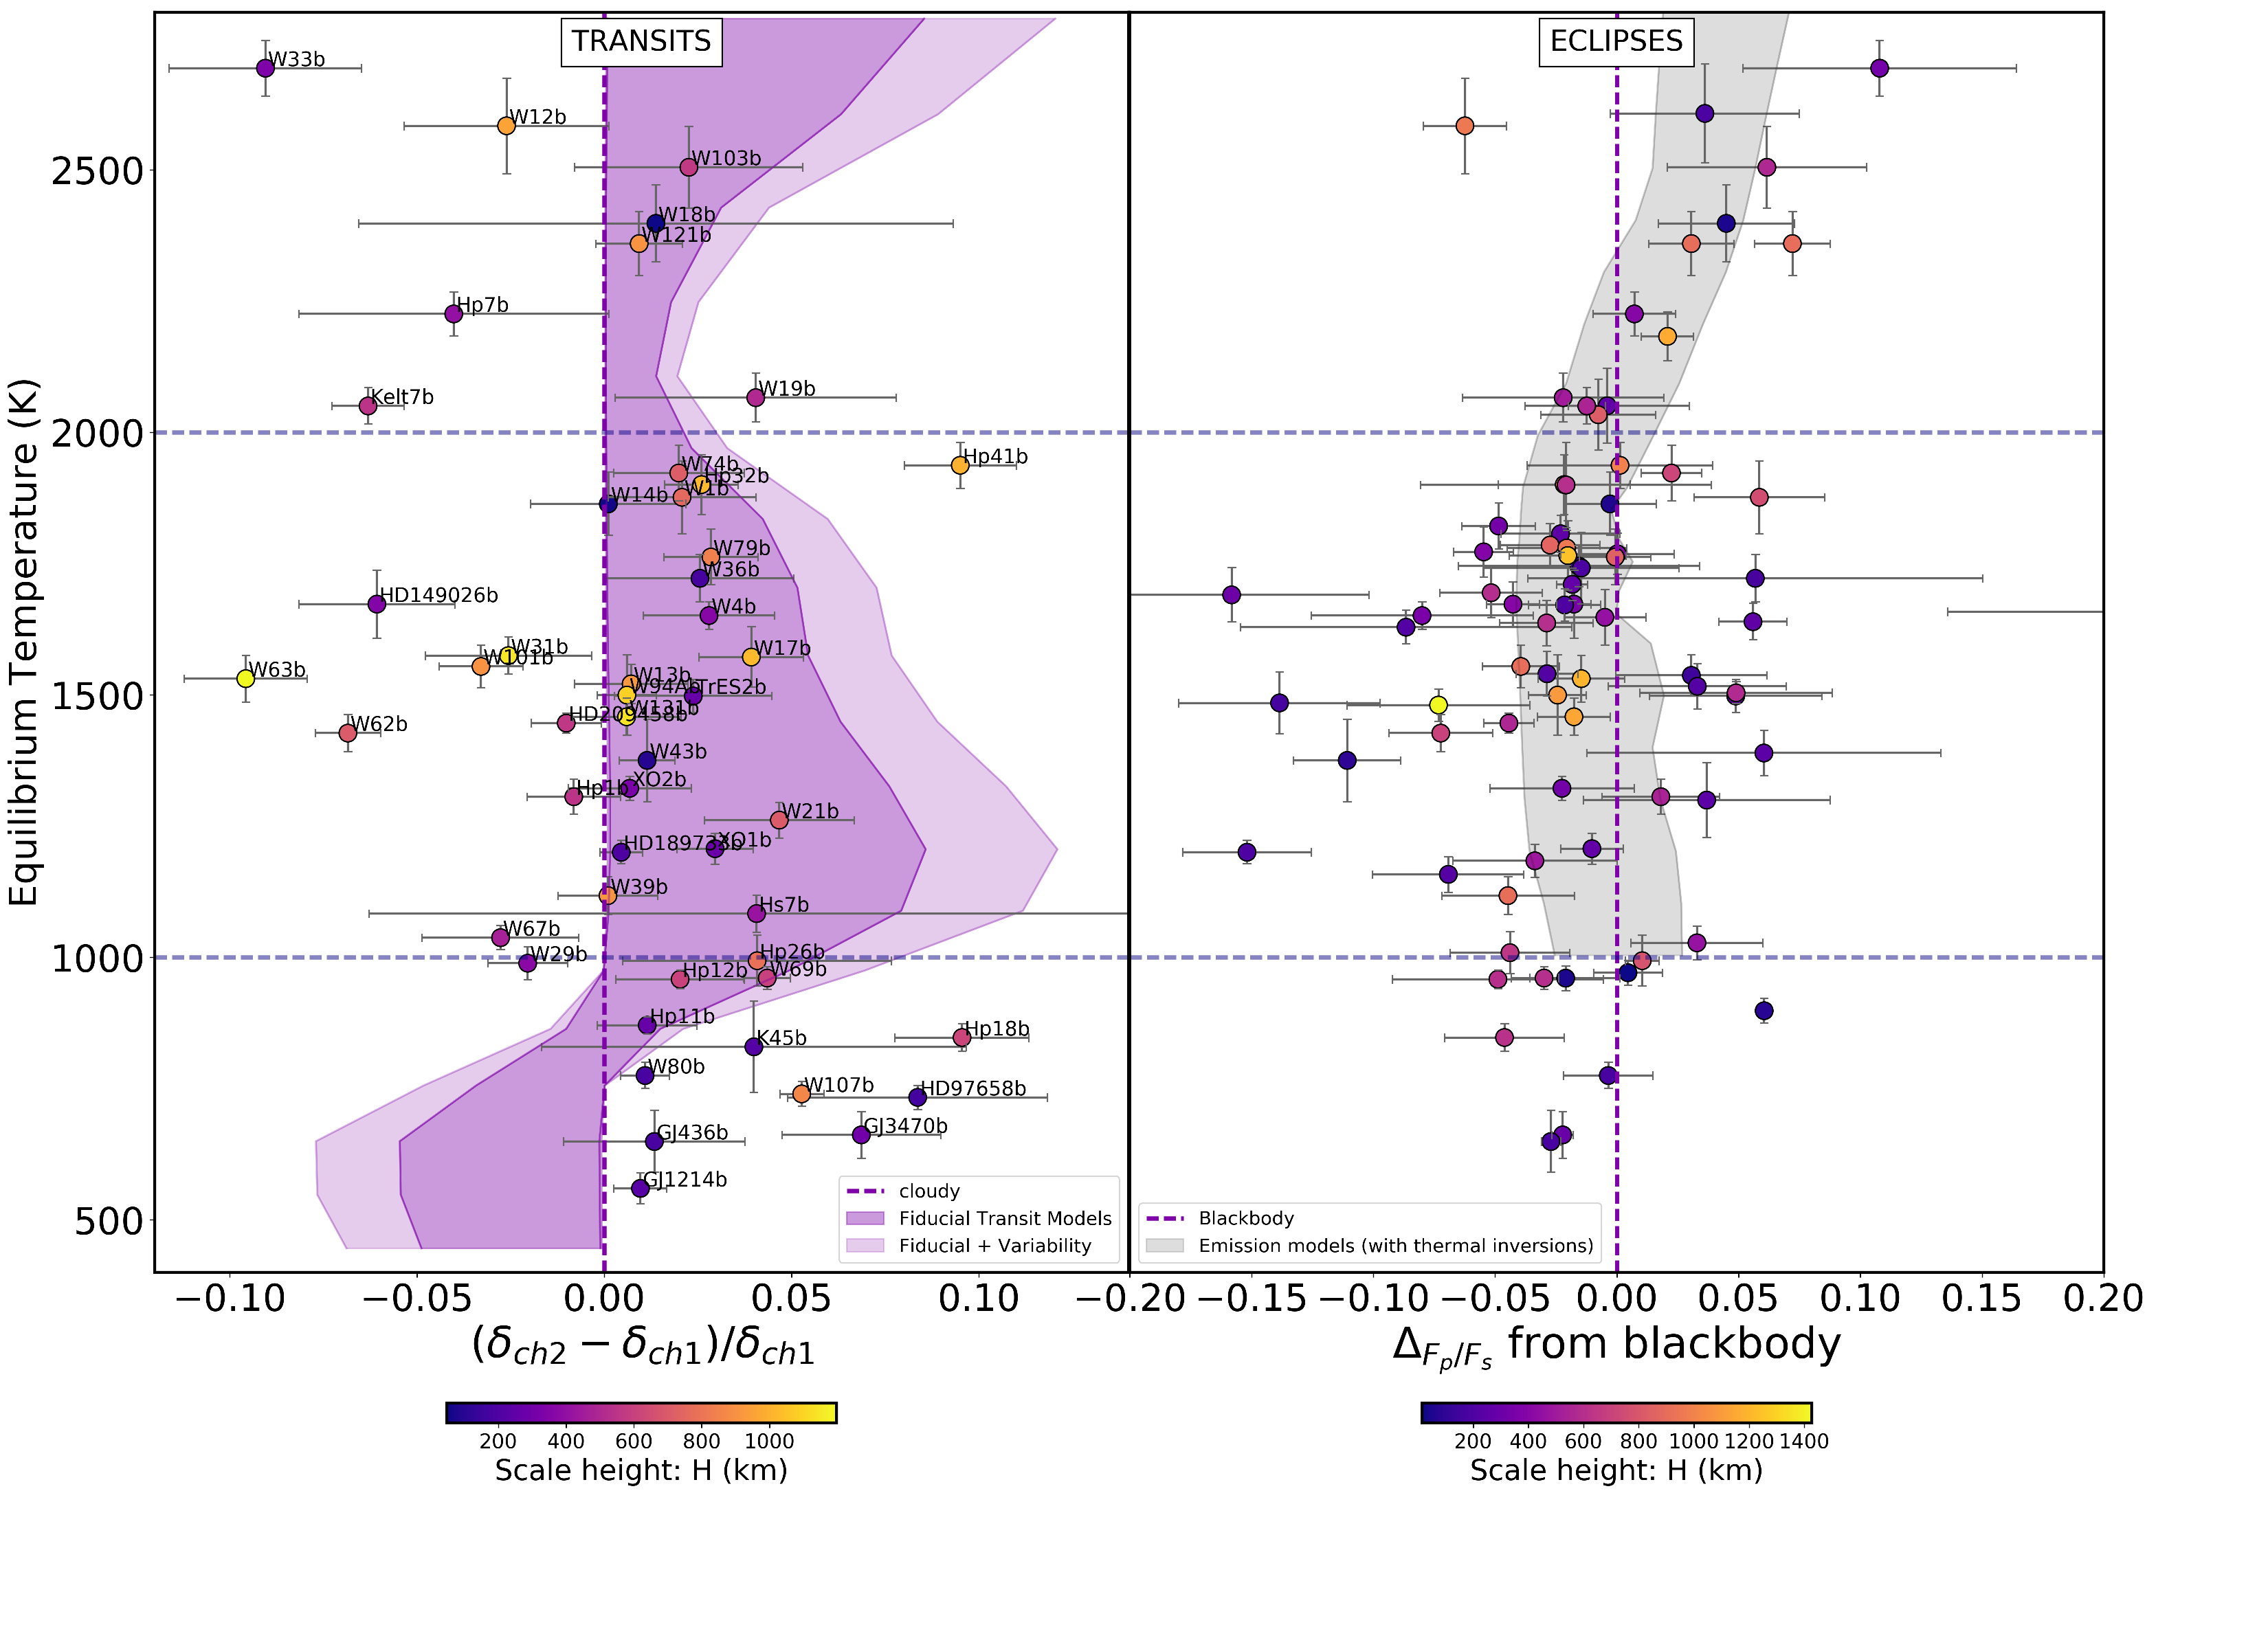
\includegraphics[trim={0 4cm 0 0},clip, width=0.8\textwidth]{UltimatePaperPlot_PHOENIX_intpl.pdf}
    \caption{Left panel: difference in transit depths between 4.5~$\mu$m and 3.6~$\mu$m normalized to the transit depth at 3.6~$\mu$m plotted against equilibrium temperature, 1-$\sigma$uncertainties are shown in gray, color bar depicts the scale height in km. The shaded area on the left panel shows our grid of solar composition cloud-free equilibrium chemistry models, the extended lighter region is corrected for stellar variability. The dashed purple vertical line at zero is where planets with low pressure gray clouds would lie. Right panel: the deviation from the blackbody in emission against the equilibrium temperature, presented in \citet{Baxter2020}. Color scale shows the scale height in km and the shaded region shows grid of models containing temperature inversions.}
    \label{P1:fig:ultimateplot}
\end{sidewaysfigure}

In Figure \ref{P1:fig:ultimateplot} (left panel), we plot the normalized transit depth difference ($(\delta_{ch2} - \delta_{ch1}) / \delta_{ch1}$) against the equilibrium temperature for all planets in our sample. This plot contains 49 planets with masses 0.02 - 10.2 $M_{jup}$, radii 0.24 - 1.9 $R_{jup}$ and equilibrium temperatures 550 - 2690 K. The color scale on the data points shows the scale height ($H$) of each planet, ($H = kT_{\rm eq}/\mu g$) calculated assuming a hydrogen dominated atmosphere with mean molecular weight ($\mu$) of 2.3, equilibrium temperature ($T_{\rm eq}$) calculated with zero albedo and zero redistribution and planetary surface gravity ($g$) from the literature.

In Table \ref{P1:tab:significance} we show the weighted mean of the normalized transit depth difference and the corresponding number of scale heights for each temperature bin in Figure \ref{P1:fig:ultimateplot}. We also calculate the weighted mean of the absolute value of the normalized transit depth difference and the number of scale heights.

We find that the weighted mean of the absolute value normalized transit depth difference and the number of scale heights to be significant to 8.0$\sigma$ and 7.5$\sigma$ respectively. This means that we are statistically detecting the atmosphere with a very high significance.

All 9 of the cool (<1000~K) planets lie on the positive side of the transit depth metric with a weighted mean transit depth of $0.029 \pm 0.007$, 4.0~$\sigma$ from zero (gray assumption). We also find that the weighted mean transit depth difference and the number of scale heights of the 1000-2000~K planets and the >2000~K planets are not significant ($<3\sigma$). We therefore treat all planets >1000~K as one sample. These 36 hot planets have an absolute value weighted mean 0.3 $\sigma$from zero (cloudy) assumption. In total, 14 of these planets are consistent with the cloudy models (zero) within 1$\sigma$. However, since these hot planets span both positive and negative values of the transit depth difference, it is unsurprising that their weighted mean transit depth is only marginally deviating from zero. The weighted mean of the absolute value of the difference in the transit depths for the hot planets is $0.025 \pm 0.004$ (5.9 $\sigma$) and is more scattered than the cooler planets.

\begin{table*}
    \centering
    \setlength{\tabcolsep}{3.5pt}
    \caption{Weighted means of the normalized transit depth difference ($(\delta_{ch2} - \delta_{ch1}) / \delta_{ch1}$), the absolute value of the normalized transit depth difference, the corresponding number of scale heights (NH), and its absolute value. This is shown for the different temperature ranges (<1000~K, 1000-2000~K, and >2000~K) presented in Figure \ref{P1:fig:ultimateplot}. The intermediate columns labeled N$\sigma$ indicate the significance of the previous weighted mean and weighted error.   }
    \label{P1:tab:significance}
\begin{tabular}{lllll}
\hline\hline
Planet Selection & $(\delta_{ch2} - \delta_{ch1}) / \delta_{ch1}$ & N$\sigma$ & $|(\delta_{ch2} - \delta_{ch1}) / \delta_{ch1}|$ & N$\sigma$ \\
\hline
All planets &   0.010 $\pm$ 0.005 & 1.9 $\sigma$ &        0.028 $\pm$ 0.003 & 8.0 $\sigma$ \\
<1000~K &        0.029 $\pm$ 0.007 & 4.0 $\sigma$ &        0.032 $\pm$ 0.006 & 5.1 $\sigma$ \\
1000-2000~K &    0.002 $\pm$ 0.006 & 0.3 $\sigma$ &       0.023 $\pm$ 0.005 & 5.0 $\sigma$ \\
>2000~K &        -0.032 $\pm$ 0.015 & 2.2 $\sigma$ &       0.042 $\pm$ 0.010 & 4.1 $\sigma$  \\
\hline \\
\hlinh\hline
Planet Selection & NH & N$\sigma$ & |NH| & N$\sigma$ \\
\hline
All planets &  0.2201 $\pm$ 0.0935 & 2.4 $\sigma$ &      0.5032 $\pm$ 0.0669 & 7.5 $\sigma$ \\
<1000~K &       0.4515 $\pm$ 0.1179 & 3.8 $\sigma$ &      0.4900 $\pm$ 0.1043 & 4.7 $\sigma$ \\
1000-2000~K &  0.0130 $\pm$ 0.1343 & 0.1 $\sigma$ &     0.4840 $\pm$ 0.0968 & 5.0 $\sigma$ \\
>2000~K &       -0.5907 $\pm$ 0.4271 & 1.4 $\sigma$ &     0.9239 $\pm$ 0.3322  & 2.8 $\sigma$ \\

\end{tabular}
\end{table*}

\subsection{Results from the 1-D grid of model transmission spectra}

\subsubsection{General trends observed in the grids of models}

\begin{figure}
    \centering
    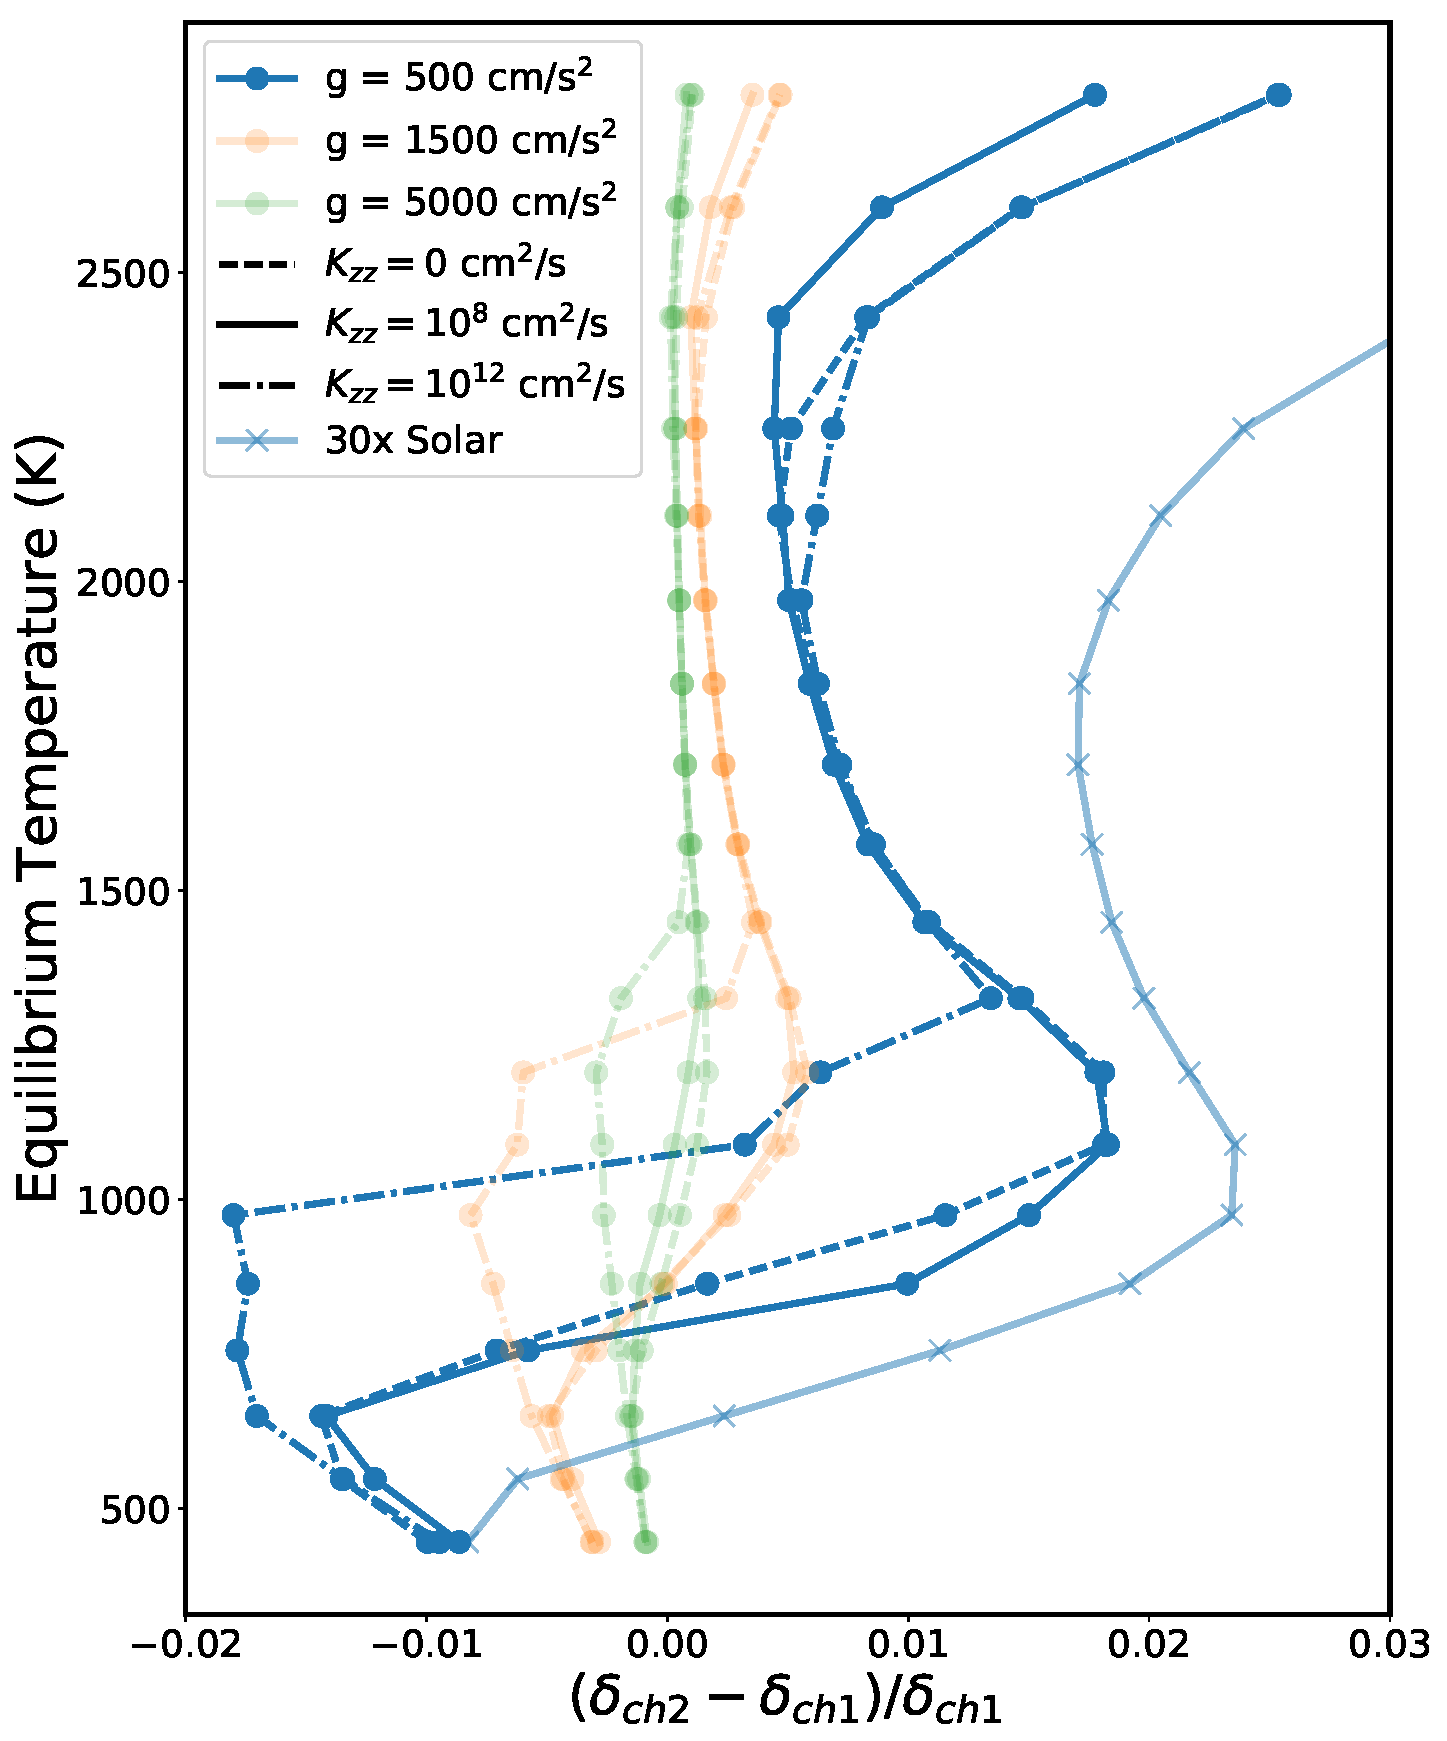
\includegraphics[width=\linewidth]{gridtracks.pdf}
    \caption{Normalized \spitzer transit depth difference as a function of the equilibrium temperature for a selection of the grid tracks created with our atmospheric model framework described in Sections \ref{P1:subsec:VULCAN} and \ref{P1:subsec:PLATON}. We show a selection of grids with 1x solar composition and $R_p = 2R_J$. Different colors show different surface gravities: blue is g = 500~\cmss, orange is g = 1500~\cmss~and green is g = 5000~\cmss. Different line styles show the effect of vertical mixing: solid line shows equilibrium chemistry, dashed is $K_{zz}=10^8$~\cmcms~and dot-dashed is $K_{zz}=10^{12}$~\cmcms. Lighter blue line with 'x' markers shows a 30x solar track with $R_p = 2R_J$, g = 500~\cmss and $K_{zz}=0$~\cmcms.}
    \label{P1:fig:tracks}
\end{figure}

\begin{sidewaysfigure}
    \centering
    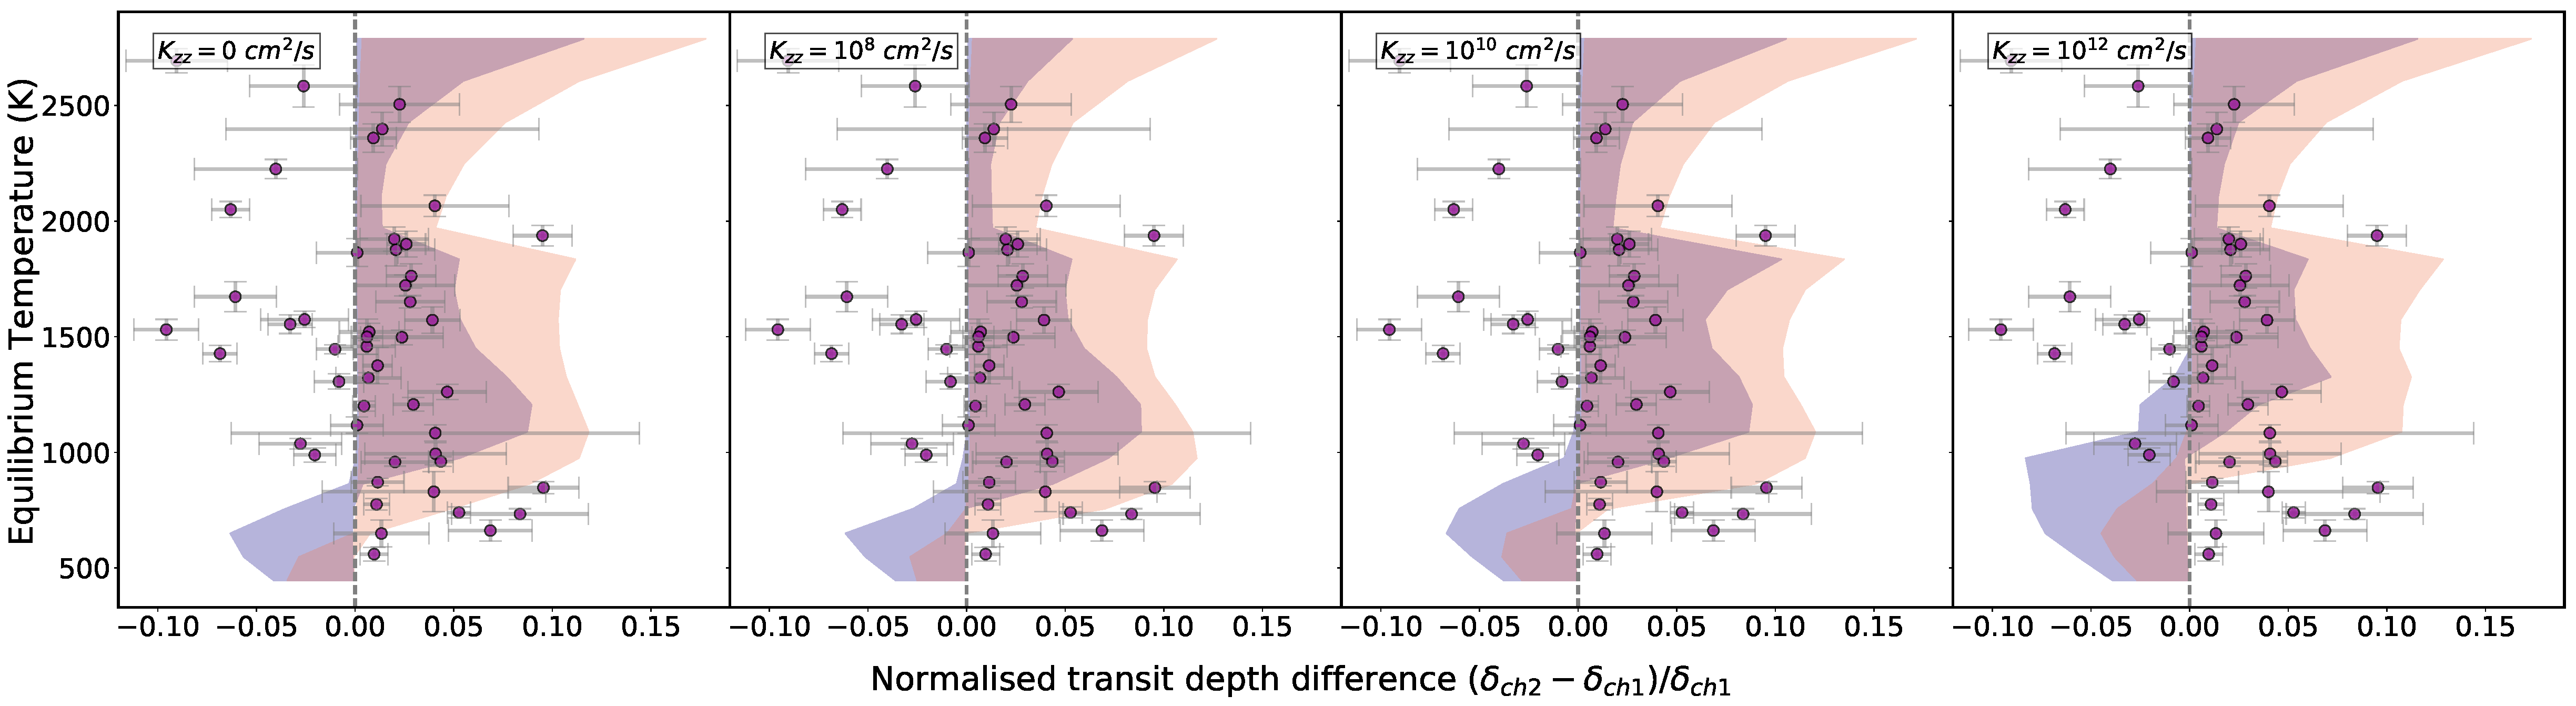
\includegraphics[width=\linewidth]{Kzzmodels.pdf}
    \caption{Normalized \spitzer transit depth difference as a function of the equilibrium temperature for the complete grids of transmission models created with our atmospheric model framework described in Sections \ref{P1:subsec:VULCAN} and \ref{P1:subsec:PLATON}. At each temperature we show the models where the surface gravity is representative of our survey, i.e. at $T_{\rm eq}>1800$~K we only plot g = 1500 and 5000~\cmss. Panels from left to right show equilibrium chemistry (no vertical mixing), $K_{zz} = 10^8$, $K_{zz} = 10^{10}$ and $K_{zz} = 10^{12}$~\cmcms. Blue translucent shaded region shows the 1x solar composition and orange translucent shaded region shows the 30x solar composition (overlap in purple). Gray dashed line represents a gray opacity source showing no spectral features. Planets from our sample are overplotted in purple circles with their $1\sigma$ errorbars.}
    \label{P1:fig:Kzzmodels}
\end{sidewaysfigure}

In Figure \ref{P1:fig:tracks} we show a selection of tracks from the complete grid of models and in Figure \ref{P1:fig:Kzzmodels} we show each interpolated grid as a shaded region in comparison with the survey data. The fiducial model grid (1x solar and equilibrium chemistry, no vertical mixing $K_{zz}=0$), plotted in Figure \ref{P1:fig:tracks} shows the effect of increasing equilibrium temperatures on the transit depths, at $\sim$900~K the model grid switches from a negative transit depth difference to a positive transit depth difference.

The interpolated grid shows a spread in the expected difference in the two transit depths. An important aspect of the model grid, which largely influences the spread is the surface gravity. Lower surface gravities result in larger scale heights and lead to a larger signal in the difference of the two \spitzerIRAC transit depths. The surface gravity also changes the shape of the TP profile as seen in Figure \ref{P1:fig:TPgrid}. Figure \ref{P1:fig:tracks} shows the effect of different surface gravities. We designed the model grid to span the parameters of the survey, notably with surface gravities of g = 500, 1000, 1500, and 5000~\cmss. However, the for ultra-hot model planets with low surface gravity of g = 500~\cmss~the upper atmosphere exceeds the Hill radius. These models do not represent any planets in our survey since the hottest planets in our survey tend to have larger surface gravity (g$\sim1000$~\cmss), we therefore discard these model planets from Figure \ref{P1:fig:Kzzmodels}.

The effect of vertical mixing can be seen in Figure \ref{P1:fig:tracks}. A large amount of mixing results in the transition between \ce{CH4} to CO occurring at higher temperatures. Increasing the metallicity to 30x solar has the effect of lowering the temperature of the transition between negative and positive transit depth difference. Increased metallicity also results in a stronger positive signal for the hotter planets >1000~K.

\subsubsection{Statistical comparison of planet atmospheres with model grid}
\label{P1:sec:gridstats}

We compare the data with the grids of models quantitatively by calculating the average number of standard deviations (based on the 1$\sigma$ uncertainties) between each of the planets and their corresponding model grid point with the closest input parameters ($T_{\rm eq}$, log($g_p$), $R_s$ and $R_p$). We then compute a weighted average for the whole grid, such that we can express the statistical significance of each grid with one number. We split this comparison into different temperature regimes based on the expected carbon chemistry. We compare the data to a transit depth difference of 0, representing a gray cloud opacity. Additionally, we also compare the data with the grids of models qualitatively by interpolating a shaded region between grid points, allowing us to visually compare the models with the \spitzerIRAC transit depth difference e.g., see Figure \ref{P1:fig:ultimateplot}.

In Section \ref{P1:subsec:TPcreation} we fix the orbital distance to 0.035 AU in our model grid creation. We do this because in our sample of planets the equilibrium temperature has a much larger correlation with the stellar effective temperature than with the semi-major axis. The range of semi-major axes in our sample spans $\sim$0.017 to $\sim$0.06 AU. We explore how much our choice of model parameterization (fixing the orbital distance to 0.035 AU) affects our results with the following two tests. We start by creating models with the minimum and maximum orbital distance of our sample, 0.017 and 0.06 AU.

In the first test, we match the equilibrium temperature by changing the effective temperature of the star. For a 650 K planet, an orbital distance of 0.017 AU corresponds to a stellar effective temperature of 3250 K and 0.06 AU corresponds to 4250 K. Figure \ref{P1:fig:Tefftest} shows the effects on chemistry, where the star with higher $T_{\rm eff}$ provides greater flux even at larger orbit and leads to more photolysis. Nevertheless, it mainly impacts the main species at the lower pressures (P < 1 mbar). We find that the resulting difference in our transit depth metric for a planet placed at the minimum and maximum orbital distance is 0.0025. This is a factor of 10 smaller than the mean errorbar in our sample, so we do not expect this to change our results.

\begin{figure}
    \centering
    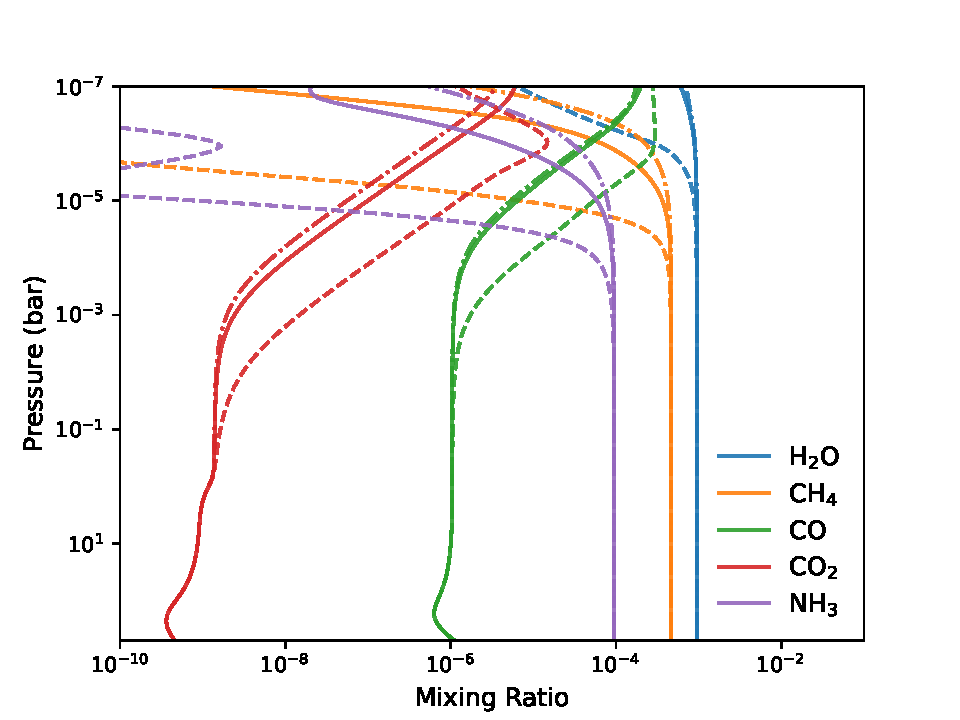
\includegraphics[width=\linewidth]{a-test.pdf}
    \caption{Abundance mixing ratios at different pressures for the main species in the \spitzer bandpasses. The solid line shows the nominal situation (a = 0.035 AU, $T_{\rm eff}$ = 3750K) dashed line shows a = 0.06 AU, $T_{\rm eff}$ = 4250K, and the dashed-dotted line shows a = 0.017 AU, $T_{\rm eff}$ = 4250K.}
    \label{P1:fig:Tefftest}
\end{figure}

In the second test, we match the equilibrium temperature by changing the stellar radius. This time the resulting difference in our transit depth metric is 3.2e-6, which is three orders of magnitude smaller than the mean errorbar of our sample. Since the changes in the models are so small compared to the size of the uncertainties, we do not expect that the different orbital distances are the reason behind the scatter seen in Figure \ref{P1:fig:ultimateplot}.

Figure \ref{P1:fig:gridstats} displays the results of the statistical comparison of each model grid with the planets in our survey. Each planet transit depth measurement is compared to the corresponding transmission model with the closest parameters ($T_{\rm eq}$, log($g_p$), $R_s$ and $R_p$). We calculate the statistical significance for a set of planets, which is quantified by the average number of sigmas, for all eight grids of models. In the two panels of Figure \ref{P1:fig:gridstats} we show the results of the cool planets ($T_{\rm eq}$<1000~K), followed by the hot planets ($T_{\rm eq}$>1000~K). We find that the hot planets are best fit by 1x solar and high vertical mixing, $K_{zz} = 10^{12}$~\cmcms. We rule out high metallicity models for these planets to $\sim3\sigma$ confidence.

On the other hand, we find that the cool planets are best fit by 30x solar and a low amount of vertical mixing ($K_{zz} = 10^{8}$ or $K_{zz} = 0$~\cmcms). We find that the 1x solar composition and high amounts of vertical mixing ($K_{zz} = 10^{12}$~\cmcms) are ruled out with $>3\sigma$ confidence for these cool planets.

We also find that the results of comparing the model grids to the full sample are that the full sample mimics the cool sample. This is because the different grids of models are divergent at the cool temperatures, so the results from the cool temperatures drive the statistical results for the full grid.

\begin{figure}
    \centering
    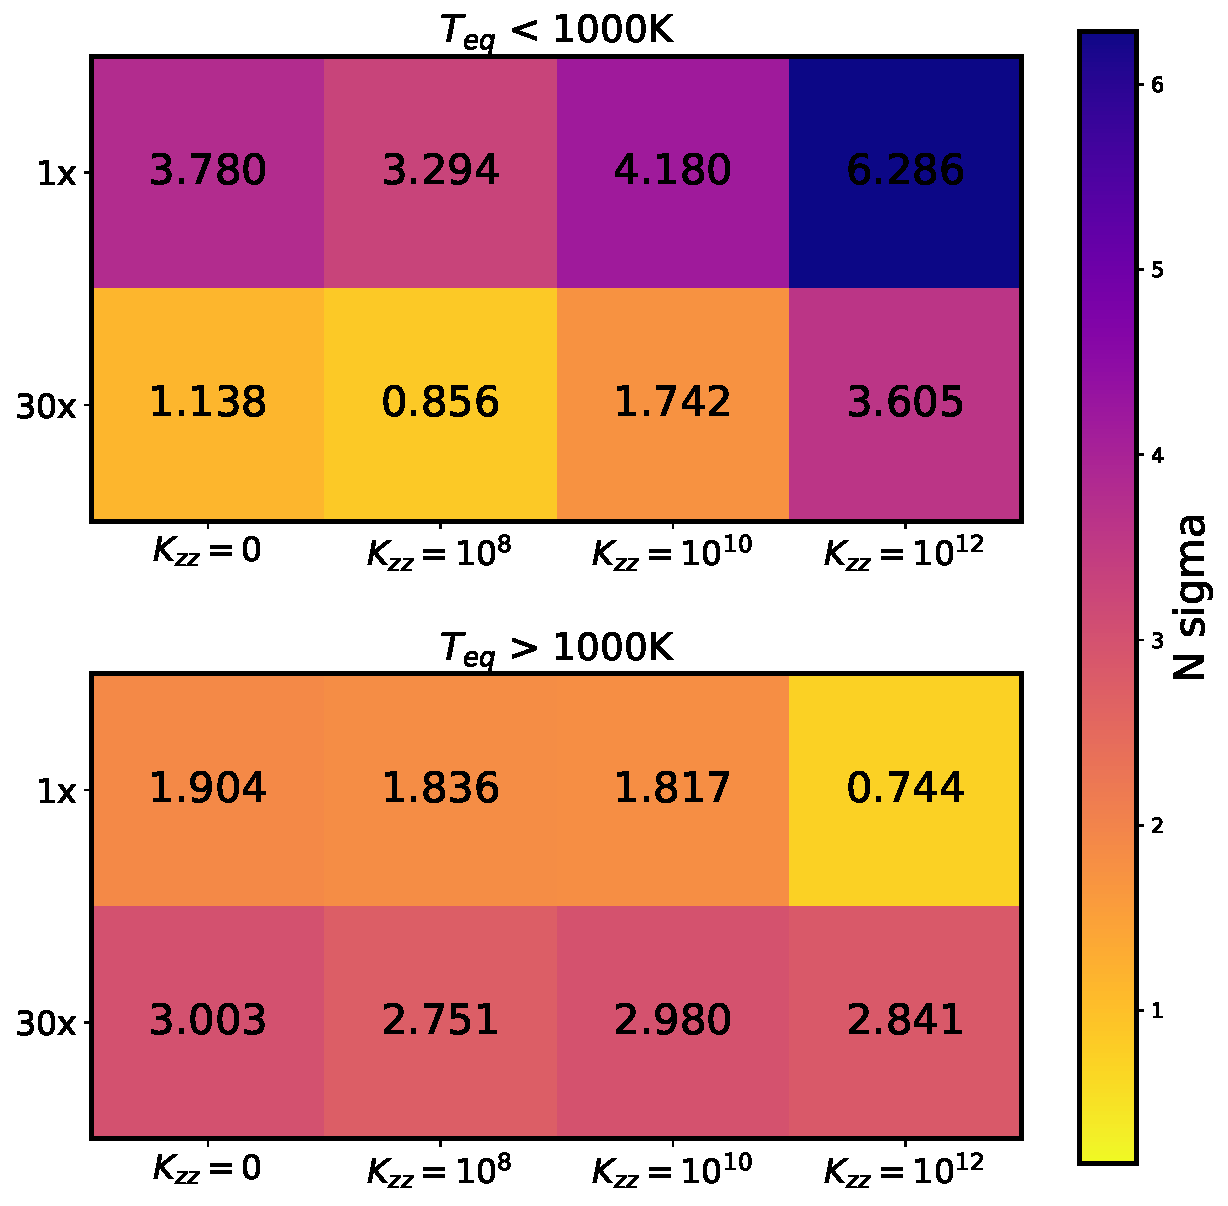
\includegraphics[width=\linewidth]{ShamiModelStatistics.pdf}
    \caption{Plot of the number of sigmas the data is from each model grid. We do this for eight grids and three sets/subsets of planets. The eight model grids are composed of two different metalicities (1x and 30x Solar) and four different vertical mixing scenarios ($K_{zz} = 0, 10^{8}, 10^{10}$ and $10^{12}$~\cmcms). The color bar represents the average number of sigmas each model grid is from the set of data, a lower N sigma (blue) means a better fit. The top panel shows the results for the cool planets ($T_{\rm eq}$<1000~K) and the bottom panel shows the  hot planets ($T_{\rm eq}$>1000~K). The number of sigmas are written on each cell.}
    \label{P1:fig:gridstats}
\end{figure}

\section{Discussion}
\label{P1:sec:Discussion}

\subsection{Expected opacities at 3.6 and 4.5~$\mu$m}
\label{P1:subsec:Chemistry}

The features we see in the transmission spectra are a result of the underlying chemistry at the pressures probed by our observations. Figure \ref{P1:fig:opacities} shows the abundance weighted opacities for the dominant opacity sources in the grid of models at the wavelengths of the \spitzer bandpasses. The dominating absorbing molecules in the \spitzer bandpasses are \ce{CH4} and \ce{H2O} at 3.6~$\mu$m and \ce{CO}, \ce{H2O} and \ce{CO2} (for high metallicities) at 4.5~$\mu$m. Since \ce{H2O} opacity is about equally present in both IRAC bandpasses, the two \spitzer transit depths can be used to understand the relative abundance of CO and \ce{CH4}. The following summary chemical reaction plays an important role in determining the dominating carbon-bearing species in an atmosphere \citep[e.g.,][]{Visscher2010, Moses2011, Visscher2011, Ebbing2016}:
\\
\ce{ \centering CH4 + H2O <=> CO + 3H2}
\\
At temperatures higher than $\sim1100$~K the forward reaction is favored (CO creation), for nominal pressures of $\sim$ 1 bar, whereas at temperatures lower than $\sim1100$~K the reverse reaction is favored (\ce{CH4} creation) \citep[e.g.][]{Madhusudhan2012, Molliere2015, Molaverdikhani2019}. The gas transition between \ce{CH4} and CO is plotted as a function of temperature on Figure \ref{P1:fig:TPgrid}, it shows where the abundance of \ce{CH4} and CO are the same \citet{Visscher2012}. A temperature pressure profile crossing this line results in CO or \ce{CH4} becoming the dominant absorber.

We thus expect that the atmospheres of planets in thermochemical equilibrium with temperatures above $\sim1100$~K have \ce{CO} as the dominating carbon bearing species and the cooler atmospheres have \ce{CH4}. The result of this on the normalized difference of the transit depths (Figure \ref{P1:fig:ultimateplot}) is that the \ce{CH4} planets would have a negative difference whereas CO planets have a positive difference. The transition from negative to positive transit depth differences seen in Figures \ref{P1:fig:ultimateplot}, \ref{P1:fig:tracks} and \ref{P1:fig:Kzzmodels} shows the changing carbon chemistry (\ce{CH4} to \ce{CO}) with increasing equilibrium temperature. We find that the equilibrium temperature of the transition in the fiducial model grid (thermochemical equilibrium, 1x solar) is slightly lower than 1100~K presented in previous work \citep[e.g.,][]{Madhusudhan2012}. We emphasize that the transition from \ce{CH4} to \ce{CO} depends on the temperature and pressure of the layer being probed with \spitzerIRAC transmission photometry, and that this temperature is not necessarily at the planet's equilibrium temperature.

\subsection{Discussion on Transit Survey}
\subsubsection{Comparing transit depths to fiducial model grid}

Figure \ref{P1:fig:ultimateplot} shows the normalized difference of the two \spitzer transit depths with the fiducial grid of models. The fiducial models are calculated with opacities from thermochemical equilibrium and 1x solar composition. The sample of planets with temperatures hotter than 1000~K follow the fiducial models, however, we see that the cool planets appear to deviate from this model grid. Since we see that different chemical and physical processes are likely occurring at these different equilibrium temperatures we proceed by splitting Figure \ref{P1:fig:ultimateplot} into three temperature regimes based on the expected chemistry from our model grid: the cooler, methane planets (<1000~K), the hotter carbon monoxide hot planets (1000~K - 2000~K) and the few ultra-hot planets where molecular dissociation can occur ($T_{\rm eq}$>2000~K).

% Cool planets
There are 13 planets in our survey with $T_{\rm eq}<$1000~K. Our fiducial (1x solar and no vertical mixing) models demonstrate that the predicted carbon-bearing species for planets in this temperature regime is methane, which results in the models occupying the negative side of Figure \ref{P1:fig:ultimateplot}. However, we find that the data show the opposite trend, all planets lie on the right side of Figure \ref{P1:fig:ultimateplot}. We find that this equilibrium chemistry grid is ruled out at 3.8$\sigma$, which is statistically capturing the dearth of methane in the sample of coolest planets, see Section \ref{P1:sec:gridstats}. This supports previous individual studies of cool gas giants with HST/WFC3 and it indicates that there are more complex physical processes happening not included in the fiducial models.

% Hot planets
There are 28 planets in the mid-temperate/hot range (1000-2000~K) and 8 planets in the hot/ultra-hot range (>2000~K) of Figure \ref{P1:fig:ultimateplot}. Of these 36 hot/ultra-hot planets, 14 of them are consistent to less than 1 $\sigma$with the cloud-free solar composition model grid. In Section \ref{P1:sec:gridstats} we show that these planets are consistent with the fiducial model grid to 2$\sigma$. Additionally, we find that there is only 1 of these 36 hot/ultra-hot planets with a stronger positive signal than the fiducial model grid, meaning that a model grid with a higher CO abundance (e.g. 30x solar) is not required to explain our sample of observations. 30x solar is ruled out with 3 $\sigma$ confidence for the hotter planets.

There are several effects not included in the fiducial grid of models which contribute to the statistical deviation. For example, we assume solar metallicity, no vertical mixing and cloud-free atmospheres. We compare the survey of planets to the model grids in a statistical manner and discuss the effects of each of these in detail below.

\subsubsection{Effect of metallicity in hot Jupiter atmospheric spectra}
\label{P1:sec:metallicitydisc}

% Metallicity
The metallicity of a planet contributes to the atmospheric molecular abundances. Our fiducial model grid assumes 1x solar composition and solar metallicity. Increasing the metallicity would increase the amount of CO in the atmosphere \citep[e.g.,][]{Venot2014}. Figure \ref{P1:fig:tracks} shows a 30x solar track and Figure \ref{P1:fig:Kzzmodels} shows the whole interpolated grid (with no vertical mixing, see the first panel). Increasing the metallicity to 30x solar results in a lower temperature at which the model atmospheres transition between \ce{CH4} and CO. This transition occurs at a temperature of around 600~K, much lower than the transition of 900~K for the fiducial grid.

In Section \ref{P1:sec:gridstats} we show that the cool planets lack the methane signature and are better fit with 30x solar composition models, with a significance of >2.5$\sigma$. This is the case for the lower values of vertical mixing ($K_{zz} = 0$,  $10^8$ and $10^{10}$~\cmcms), discussed in more detail in Section \ref{P1:sec:Kzzdisc}. These cool planets are also generally lower mass planets because of the detection biases for these systems, see Figure \ref{P1:fig:planets}. Lower mass planets typically have higher metallicities \cite{Fortney2013, Welbanks2019}. Therefore, a higher average metallicity in the 13 planets with temperatures <1000~K likely explains the lack of methane. Our findings support the predicted high metal enrichment in cool gas giants presented in \citet{Espinoza2017}. They predict C/O ratios for a sample of 50 gas giants with $T_{\rm eq}<1000$~K, 6 of our 13 planets in this temperature range are also in their sample. Furthermore, our finding of high metallicity for these coolest warm giant planets supports the individual high metallicity measurements of several planets in the literature: HAT-P-12b \citep{Line2013b}, HAT-P-26b \citep{Wakeford2017}, GJ 436b \citep{Morley2017} and HAT-P-11b \citep{Mansfield2018b}.  All of these exoplanet atmospheres are found to have super-solar metallicities, except for GJ 3470b which is suggested to have a relatively low atmospheric metallicity for its planet mass \citep{Benneke2019}.

On the other hand, the planets with equilibrium temperatures >1000~K are consistent with the 1x solar composition models to less than 2$\sigma$ for all values of $K_{zz}$. The higher metallicity grid is less favored for these planets (2.6$\sigma$ deviation). Similar to the high abundance of CO at cooler temperatures, the high metallicity model grid shows stronger CO features throughout the entire temperature range, which is not favored by the planets in our survey. We do not find it necessary to statistically invoke high metallicity to explain the near-infrared spectral features of hot Jupiters.

Figure \ref{P1:fig:opacities} shows the opacities for the 1x and 30x metallicity used in the creation of our model grids. In practice, differences in the opacities for the two cases would also affect the temperature pressure profile, however, in our analysis we do not compute the temperature pressure profiles self consistently. Nevertheless, we can predict what effect this might have. Higher metallicities would result in hotter temperatures in our TP profiles, which would in turn result in a larger \ce{CO}/\ce{CH4} ratio. This means that we could explain the dearth of methane with less extreme enhancements in the metallicity of the models.

\subsubsection{Vertical mixing and non-equilibrium effects}
\label{P1:sec:Kzzdisc}

Another aspect not included in our fiducial model grid is the presence of non-equilibrium effects such as photochemistry, advection, convection, and turbulence in the atmosphere. To capture some of these non-equilibrium atmospheric processes, we introduce an eddy diffusion coefficient, $K_{zz}$, into our modeling (see Section \ref{P1:subsec:VULCAN}). Theory suggests that for hot Jupiters $K_{zz}$ can range from $10^8$ to $10^{12}$~\cmcms~based on the estimation from the mean vertical wind in GCMs \citep{Moses2011}. We create four different grids of models spanning the range of eddy diffusion coefficients: equilibrium chemistry, $K_{zz} = 10^8$, $K_{zz} = 10^{10}$ and $K_{zz} = 10^{12}$~\cmcms.

The model incorporating different $K_{zz}$ show that the transition between \ce{CH4} and CO being the dominating carbon bearer in these atmospheres occurs at higher temperatures for larger values of $K_{zz}$. This is because with larger values of $K_{zz}$, the mixing penetrates deeper into the atmosphere and can therefore dredge up methane to the observable pressures of hotter planets where methane is not expected. The models on Figure \ref{P1:fig:Kzzmodels} (right panel) demonstrate that $K_{zz} = 10^{12}$~\cmcms~can dredge up \ce{CH4} for planets up to 1300~K.

For the cool planet data (T<1000~K), we find that the models containing low amounts of vertical mixing are significantly favored over high vertical mixing for both metallicities. For 30x solar metallicity, the low mixing $K_{zz}$ = $10^8$~\cmcms~fits marginally better than equilibrium chemistry ($K_{zz}$ = 0) and is a 3$\sigma$ better fit than the high vertical mixing ($K_{zz}$ = $10^{12}$~\cmcms). On the other hand, for the hot planets we find that $K_{zz}$ = $10^{12}$~\cmcms~is favored over the lower mixing or no mixing for both the 1x and 30x solar metallicities.

\citet{Komacek2019} showed that for tidally locked hot Jupiters, vertical mixing increases with increasing equilibrium temperature and rotation rates: starting at $K_{zz} = 10^{7}-10^{8}$~\cmcms~for the coolest (500~K) planets and going to $K_{zz} = 10^{11}-10^{12}$~\cmcms~for the hottest (1500-3000~K). We find that the cool planets support these results, with a vertical mixing of $K_{zz} = 10^{8}$~\cmcms~favored by the data. However, the hotter planets seem to suggest a lower level of mixing than theory predicts, our models with $K_{zz} = 10^{10}$~\cmcms~are marginally supported over the equilibrium and $K_{zz} = 10^{8}$~\cmcms~grids, which is lower than the theoretical maximum of $K_{zz} = 10^{12}$~\cmcms. These findings are in line with the findings of \citet{Miles2020} for non-equilibrium processes in brown dwarfs. They found warmer brown dwarfs showed lower mixing than theory predicts, yet the cooler objects were close to the theoretical maximum.

Additionally, our non-equilibrium chemistry models include the effects of photochemical reactions. For hot planets ($T_{\rm eq}$ > 1000 K), CO is only dissociated in the upper atmosphere due to its strong bond, which has negligible influence on the \spitzer bandpasses. For cooler planets ($T_{\rm eq} \leq$ 1000 K), \ce{CH4} is dissociated by atomic hydrogen produced by photolysis. This destruction of \ce{CH4} can penetrate down to around 0.1 mbar with lower mixing ($K_{zz}=10^{8}$~\cmcms). Yet the competing effects of mixing can overtake and efficiently transport methane to the upper atmosphere. HCN is also produced by photochemistry and can reach abundances close to CH4 in some cases. Nevertheless, HCN absorbs similarly at the two IRAC wavelengths, so we do not expect that it would have significant effects on the normalized transit depth difference.

Since vertical mixing is responsible for dredging \ce{CH4} to the hotter planets, and not CO in the cooler planets, we conclude that the dearth of methane is not due to strong atmospheric mixing, it is likely due to the higher metallicity of these atmospheres. Another possible factor affecting the lack of methane signatures in the cool planets could be the amount of interior heating, see \citet[e.g.,][]{Fortney2020}. We find that several of the coolest planets are eccentric (see Table \ref{P1:tab:jumpParams}, which could cause some tidal heating. Our temperature pressure profile calculation assumes an interior heating of $T_{\rm int}= 150$~K. However, substantial interior heating, $T_{\rm int}$>300~K, could result in pushing the deeper layers of these atmospheric TP profiles towards the CO regime \citep{Morley2017, Benneke2019, Thorngren2019, Thorngren2020}. If the interior is more CO dominated, then vertical mixing could dredge up CO in the cooler planets, resulting in a dearth of methane \citep[e.g.,][]{Moses2013a}. We did not test this as it is beyond the scope of our paper.


\subsubsection{Effects of clouds on the cool and hot Jupiter atmospheric spectra}

Clouds are ubiquitous in transiting exoplanet atmospheres \citep{Sing2016}.
There are several mechanisms responsible for producing homogeneous and inhomogeneous clouds on tidally locked planets \citep{Parmentier2013, Parmentier2021, Helling2016, Helling2019a, Helling2019b}.
An example can be found in \citet{Line2016a} in which HD 189733b and HAT-P-11b can be explained by patchy clouds without the need to invoke global clouds or high mean molecular weight atmospheres.


% cool clouds
Hazes are expected to be prominent in the cooler atmospheres. \citet{Morley2015} predicted that a transition between haze-free and hazy atmospheres will occur at 800-1100~K, implying that any planet below this temperature might show no molecular features. \citet{Gao2020} showed that the amplitude of the HST/WFC3 water feature on planets with temperatures <900~K is such that these atmospheres become dominated by haze formation. However, \citep{Kawashima2019} predict that molecular features such as CO and \ce{CH4} are still detectable in the infrared for their sample of warm Jupiters (<1000~K) with hazy atmospheres.

Furthermore, if all planets with temperatures <1000~K in our survey were characterized by a gray cloud opacity, then we would expect the the transit depth difference to be evenly distributed around zero in Figure \ref{P1:fig:ultimateplot}. However, these 13 planets have a mean transit depth of $0.026 \pm 0.008$. This rules out a gray cloud (flat spectrum) at 4.0~$\sigma$ confidence for all planets. Suggesting that these planets cannot be characterized by a gray cloud opacity, and that there is a molecular feature.

\citet{Molaverdikhani2020} suggested that clouds could play a role in the heating of the atmosphere, resulting in a lack of \ce{CH4}. However, such clouds would also dampen the \ce{CO} feature significantly. This effect could be the reason for the few planets consistent with zero, but we do not expect that this effect explains the 4.0$\sigma$ detection for the sample of cool planets (<1000~K).

% hotter clouds
There are 14 planets with equilibrium temperature >1000~K that have transit depth differences consistent with zero (flat spectrum). The weighted mean transit depth difference of all these planets is -0.002 $\pm$ 0.006, only 0.3$\sigma$. However, the weighted mean of the absolute value of the transit depth difference is 0.025 $\pm$ 0.004 (5.9$\sigma$).


Based on the prediction by \citet{Morley2015} we would not expect to have hazes at these temperatures. However, \citet{Gao2020} show that the HST water feature is dampened when compared to a cloud-free atmosphere, and they find the data is better fit by their models containing silicate clouds. Furthermore, \citep{Line2016a} suggested that patchy cloud cover can mimic the spectral features of a high mean molecular weight atmosphere, resulting in a flatter transmission spectrum. Additionally, due to the varying temperature across the day and night sides of tidally locked highly irradiated hot Jupiters, clouds and hazes may behave differently at the east and west terminators of the planet \citep{Kempton2017b}. Such that photochemically generated hazes formed on the day side can be blown over to the nightside and dampen the transmission features. We therefore expect that clouds do play a role in dampening the spectral features in some of our planets, namely, those in the temperature region predicted to be cloudy by \citet{Gao2020} (>1000~K).

However, since there is still a strong signal in the absolute value of the transit depths of these planets (5.9$\sigma$), there is indication that the population cannot be captured by a completely featureless model. Mie scattering theory results in a drop off in cloud opacity at ~2-3~$\mu$m \citep[e.g.,][]{Benneke2019}, since we are detecting molecular features between 3-5~$\mu$m it may be that any possible cloud particles could exhibit Mie scattering in this regime. Including Mie scattering as a cloud prescription in our transmission spectrum forward modeling is beyond the scope of this paper. However, since the cloud opacity would be lower at 4.5~$\mu$m than it is at 3.6~$\mu$m, it would result in a negative transit depth metric, similar to the expected methane signature. However, we do not find planets with a negative transit depth metric, and hence find no evidence for Mie scattering clouds.


\subsubsection{Outliers and the effect of nightsides}
\label{P1:subsec:additionaleffects}

% Outliers
According to our grids of models, we do not expect any of the planets above 1400~K to have \ce{CH4} as the dominating carbon bearing species in any of the metallicity or mixing scenarios. However, there are two hot planets which are significantly on the left: HD149026b and WASP-33b (2.9$\sigma$ and 3.5$\sigma$ from zero respectively). HD 149026b has previously been discrepant from models, for example, \citet{Zhang2018a} found that they needed 30x solar metallicity to reproduce the \spitzer 3.6 and 4.5~$\mu$m phase curves. Furthermore, the biggest outlier, WASP-33 b, is a planet that is orbiting a $\delta$ Scuti star, with pulsating periods close to the transit duration \citep{Herrero2011}. Both of these planets indicate that there may be additional factors that could significantly affect the transit light curves, however, statistically it is not unexpected to have a couple of outliers. In Section \ref{P1:sec:stellarVariabilitiy} we discuss how we treat stellar variability for the whole survey.

Additionally, three of the seven hottest planets above 2000~K (WASP-33b, WASP-121b, and WASP-18b) have evidence of a temperature inversion \citep{vonEssen2015, Haynes2015, Evans2017, Arcangeli2018}. However, since transmission spectroscopy is not as sensitive to the temperature profile at low resolution \citep[e.g.,][]{Brown2001} so we do not expect to see the effect of temperature inversions in the transit depth difference of the two \spitzerIRAC bandpasses. Additionally, the \ce{H-} opacity seen at the WFC3 bandpass \citep[e.g.][]{Arcangeli2018} does not become important at the \spitzerIRAC bandpasses until equilibrium temperatures as high as 3500~K.

\subsubsection{Radius Anomaly}

Our sample subsequently spans a very large range of scale heights, ranging from HAT-P-2b with a scale height of 26~km to WASP-31b with a scale height of 1150~km. Figure \ref{P1:fig:ultimateplot} demonstrates that there is no trend with the atmospheric scale height and the strength of the spectral features indicated by the magnitude of the transit depth metric. Furthermore, the radius anomaly is thought to correlate with incident flux, with hotter planets having a more inflated radius \citep{Thorngren2018}. However, we do not find a trend with the radius anomaly and the strength of the spectral features seen with \spitzer (see Figure \ref{P1:fig:RadiusAnomaly}).

\subsubsection{Stellar Variability}
\label{P1:sec:stellarVariabilitiy}

Contamination of the transmission spectrum from starspots, faculae and flares generate brightness temperature differences between the disk-integrated spectra of the star and the region occulted by a transiting planet \citep{Desert2011d, Pont2008, Sing2011}. If a planet occults a star spot at a different temperature to the photospheric one, it can change the shape of the lightcurve by appearing as a change in the flux during transit. On the other hand, if the star spot is not occulted, then the disk integrated spectrum of the star is  fainter or brighter, depending on the spot properties, which can cause the measured transit depth to be different than the nominal one. Stellar variability can occur when star spots rotate in and out of view of the integrated stellar disk, which depends on the rotation period of the star.

To estimate the possible effect of stellar variability on our results, we aim to provide a quantitative estimate of how this would affect the sample as a whole, by expanding the interpolated model grid. We do this by looking at a worst case scenario variable star, HD 189733, which has a peak-to-peak variability of $\sim 3$\% in the visible \citep{Henry2008}. We follow the method in \citet{Desert2011d, Sing2011} and \citet{Berta2012} to calculate the effect of this variability on the transit depth metric. We first translate this 3\% in V-band to 0.8\% at 3.6~$\mu$m using the ratio of blackbodies, we set 2.8\% spot coverage with spots at 1000~K less than the stellar photosphere. We can propagate this to a relative error on the transit depth and assuming it will affect 4.5~$\mu$m as much as 3.6~$\mu$m (in reality it will be a smaller effect), we can then propagate this to an error on the transit depth metric ($\delta_{ch2} - \delta_{ch1} / \delta_{ch1}$). This leads to a 42\% maximum error on the transit depth metric, we thus extend the models positive and negative by this percentage, which is plotted on Figure \ref{P1:fig:ultimateplot}.

Despite choosing the worst case scenario to expand our model grid, the features arising from the changing chemistry with equilibrium temperature can still be clearly distinguished in the grid of models in Figure \ref{P1:fig:ultimateplot}, i.e. the transition regions at $\sim1000$~K and $\sim 2200$~K remain clear. The relative size of the variability region is on average one-third of the size of the average uncertainty on the data points. Nevertheless, this is a conservative upper estimate and will not apply as strongly to all planets in our sample, since not all stars are as variable as HD 189733. If the temperature difference between spot and photosphere is less or if the spot covering fraction is smaller, then this would result in a lower variability amplitude and smaller effect on the transmission spectrum. Additionally, 3\% is the maximum peak-to-peak variability, this would only apply if the observations where taken at the peak and trough of the variability period. Since we designed the observations to have as few orbital periods as possible to be within one variability period of the star, it is unlikely that we reach the maximum variability between our two \spitzer observations.

\subsection{Comparing Transmission and Emission with warm \spitzerIRAC}
\label{P1:sec:TvsE}

Several of the planets from our survey have published secondary eclipse measurements. We utilize the secondary eclipse literature survey from \citet{Baxter2020} (and references therein) which contains 3.6~$\mu$m and 4.5~$\mu$m eclipses for 78 planets in total. Several of the eclipse depths presented in Table 1 of \citet{Baxter2020} were taken from \citet{Garhart2020}, and some of these planets had dilution corrections due to companions in the field of view. The dilution corrections were applied before any analysis in \citet{Baxter2020}, but this was not reported in their Table 1. We have thus reported the eclipse depths with dilution corrections in Table \ref{P1:tab:eclipses} of this work using the dilution correction factors presented in Table 4 of \citet{Garhart2020}. We use the eclipse depth, equilibrium temperature, brightness temperatures at 3.6~$\mu$m and 4.5~$\mu$m and the deviation from the blackbody presented in \citet{Baxter2020}. The deviation from the blackbody probes the temperature pressure profile. A positive deviation is either methane in absorption at 3.6~$\mu$m with a nominal TP profile or CO in emission at 4.5~$\mu$m if the TP profile is inverted. Twenty-four of the planets in \citep{Baxter2020} are also in our transmission survey, which allows us to statistically compare the two samples. To better understand the dearth of methane planets presented in Section \ref{P1:sec:gridstats}, we compare the difference in brightness temperature from emission with the normalized difference in transit depths for planets with both emission and transmission observations. Additionally, we create a color-magnitude plot and compare the emission to the brown dwarf spectral sequence with a focus on the coolest planets.

\subsubsection{Probing different pressures with emission and transmission}
\begin{figure}
    \centering
    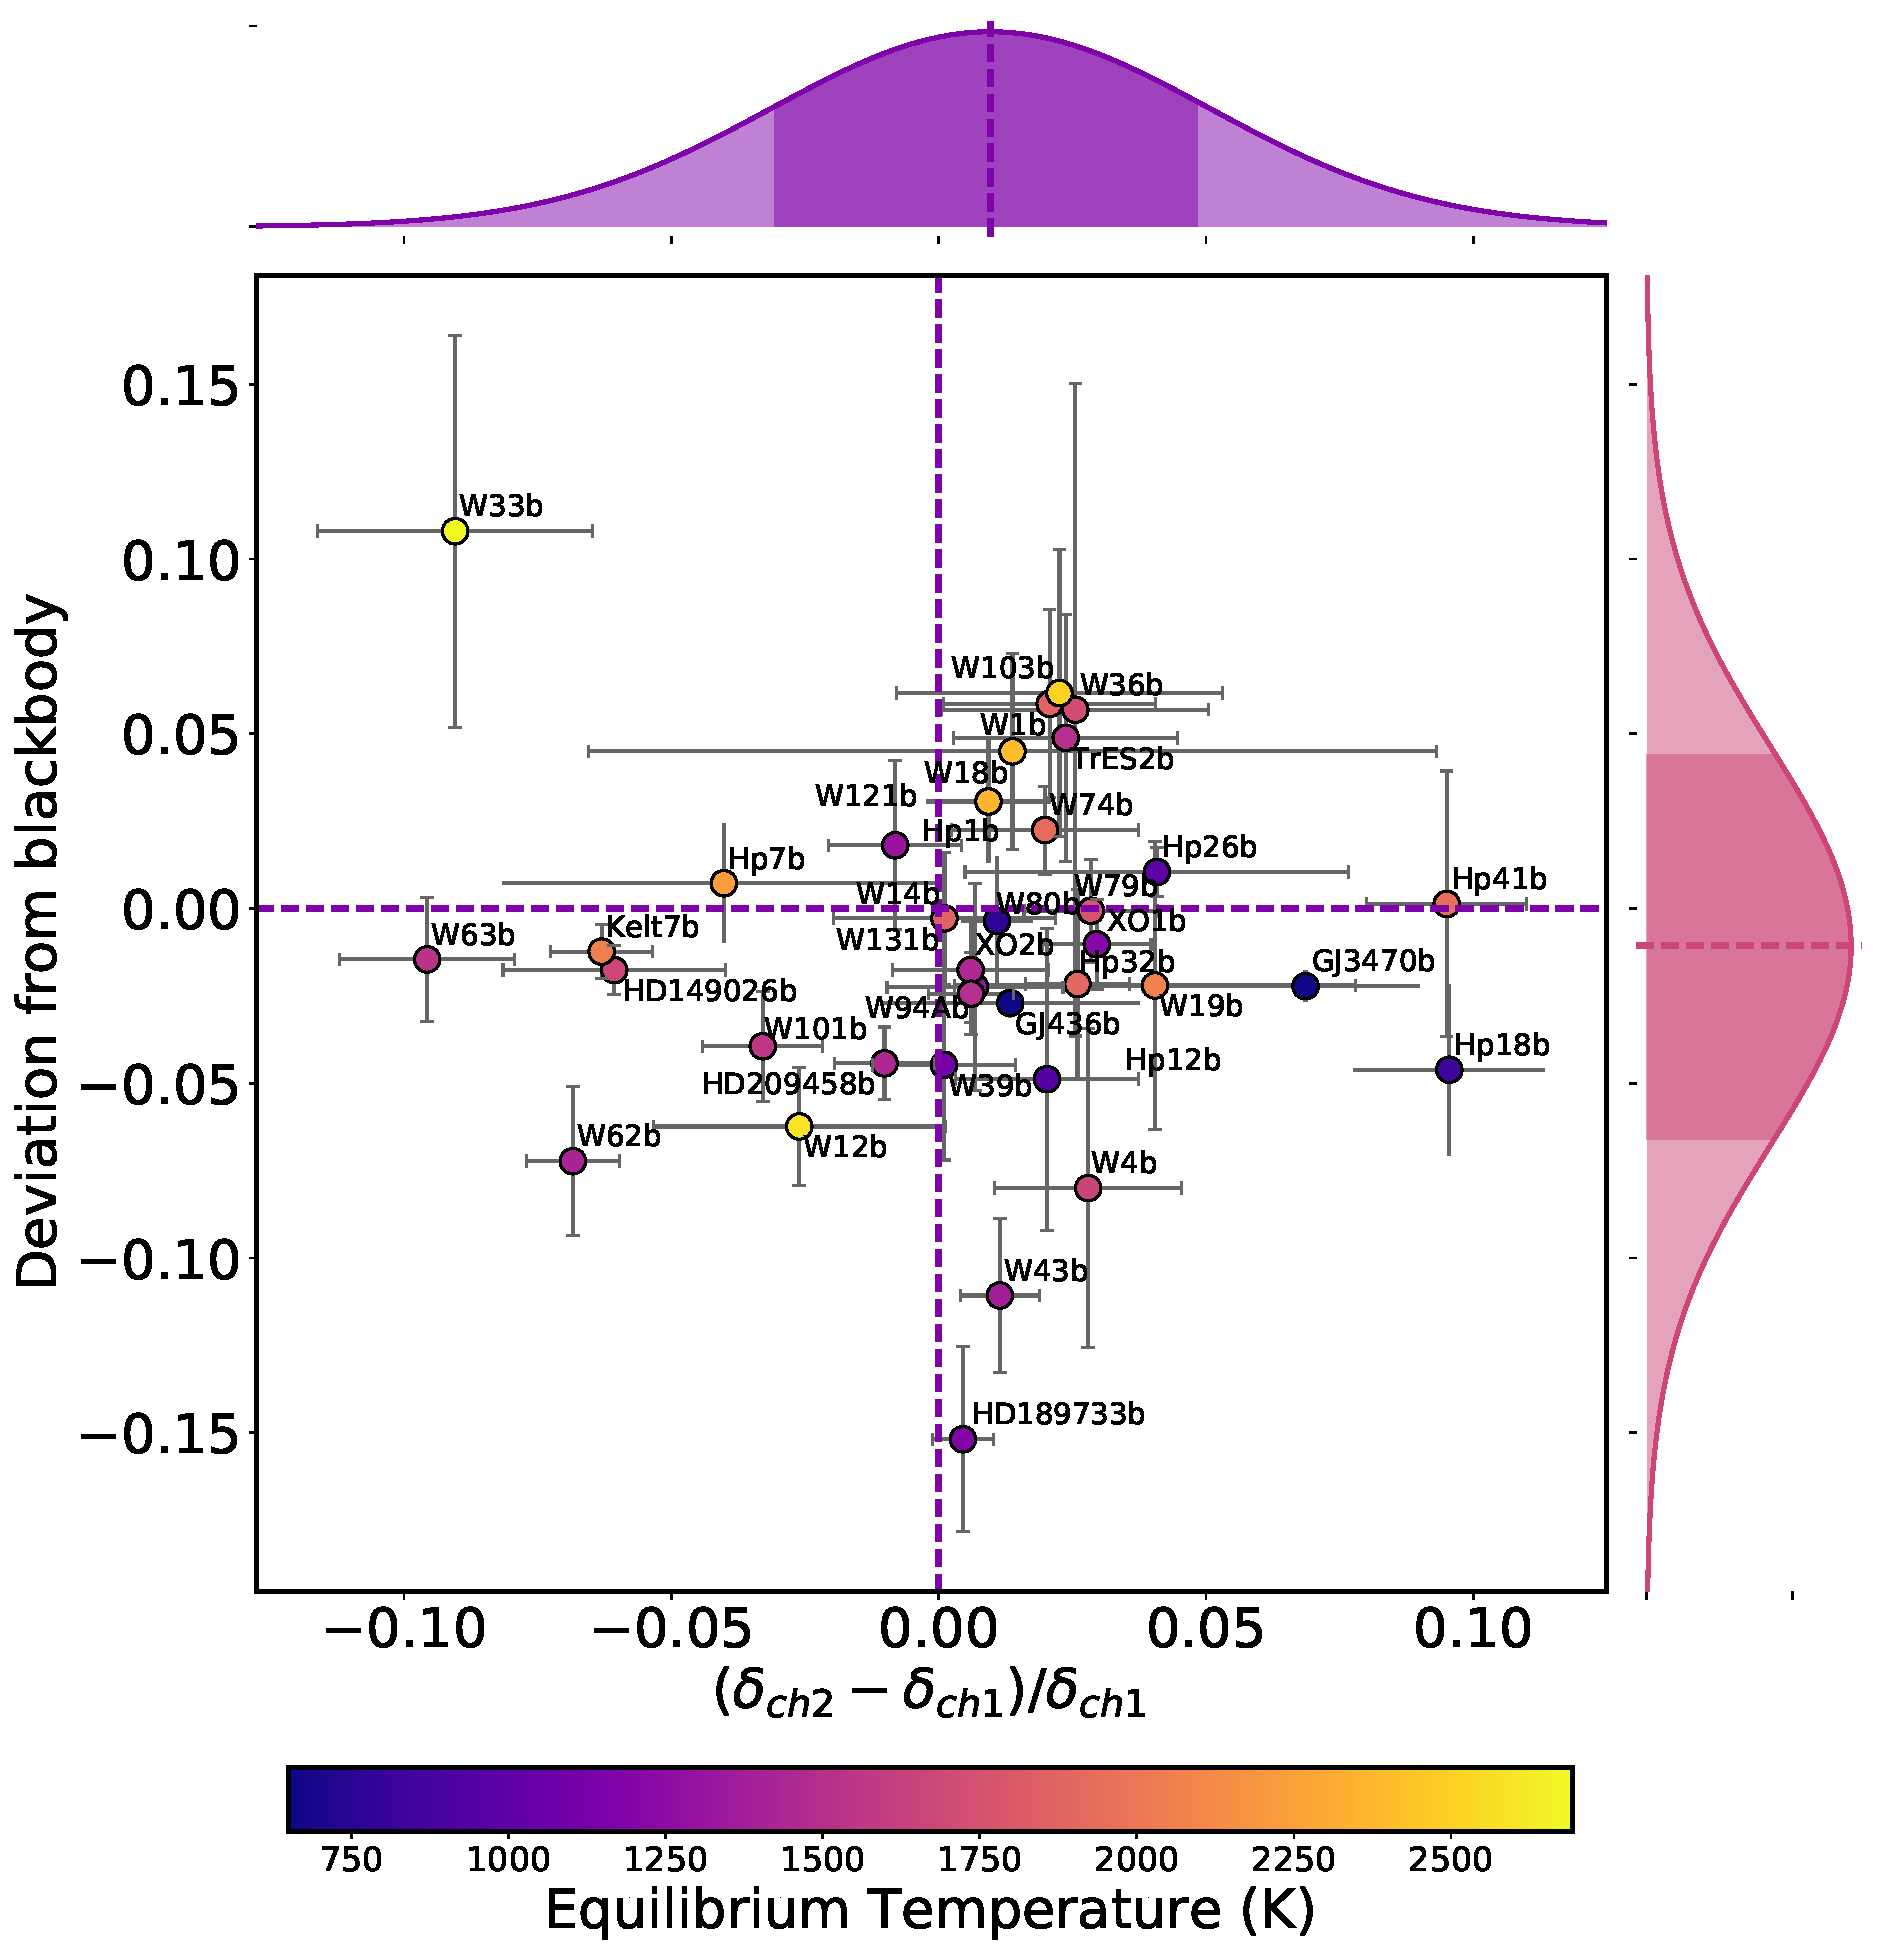
\includegraphics[width = \linewidth]{TvsE+hist+emily.pdf}
    \caption{Deviation from a blackbody calculated from emission against the normalized difference in the transit depth presented in Figure \ref{P1:fig:ultimateplot}. Histograms on each axis show the mean and standard deviation of each axis. The equilibrium temperature of each planet is shown with the color scale.}
    \label{P1:fig:TvsE}
\end{figure}

In \citet{Baxter2020}, we demonstrate that the relative opacities in the two \spitzerIRAC bandpasses can act as a probe of the atmospheric temperature structure when observing the dayside emission. The deviation from blackbody metric described in \citet{Baxter2020} plotted against the equilibrium temperature shows that ultra-hot Jupiters have statistical evidence for thermal inversion. In a non-inverted atmosphere, a positive deviation indicates that the 3.6~$\mu$m brightness temperature is lower than that at 4.5~$\mu$m due to methane absorption at 3.6~$\mu$m and a negative deviation indicates that the 4.5~$\mu$m $T_b$ is lower due to CO absorption at 4.5~$\mu$m. On the other hand, if the atmosphere is inverted, CO being the dominating carbon bearing species in the atmosphere would result in a positive deviation due to seeing CO in emission at 4.5~$\mu$m. In this work we are focusing on the \ce{CH4} to \ce{CO} transition temperature and thus we do not account for temperature inversions.

In Figure \ref{P1:fig:TvsE} we compare the difference of the two IRAC brightness temperatures against the normalized difference in the transit depth. There appear to be no trends in the emission and transmission of the planets in our survey with both eclipses and transits, and we also find that the top left quadrant is almost empty, with the main outlier being WASP-33b. Given that the deviation from the blackbody can be positive or negative for a CO dominated atmosphere depending on the TP profile, we test for trends in the planets with equilibrium temperatures below 1800~K, which are not expected to have thermally inversions in their atmospheres. We find that the top left quadrant, which indicates \ce{CH4} in transmission and \ce{CH4} in emission, is empty. Meaning that any planets which show signs of methane in either emission or transmission do not show it in the other. For example, HD 149026b lies in the bottom left quadrant, it has a negative deviation from a blackbody, which indicates a CO absorption feature in emission (assuming a non-inverted TP profile). The expected corresponding transmission spectrum would predict a positive transit depth difference. However, this is not what we see. Possible reasons for these differences include: longitudinal abundance differences, more complex atmospheric processes such as atmospheric mixing, different cloud composition/abundances at different layers in the atmosphere, or changes in the thermal structure between emission and transmission \citep[e.g.,][]{Fortney2005}. Additionally, similar to the results for the planets in transmission, we do not find a correlation between the deviation of the blackbody and the radius anomaly.


\subsubsection{Comparing to brown dwarfs with a Color-Magnitude diagram}


We create also a color-magnitude plot using these \spitzer secondary eclipses. Our work expands on that presented in \citet{Triaud2014c} by extending their survey from 37 planets to the 78 planets presented in \citet{Baxter2020} and by using the newly released GAIA dr2 for more accurate distances \citep{GaiaCollaborationandBrown2018}. We calculate the planetary apparent magnitudes by using the apparent stellar magnitudes from the WISE spacecraft \citep{Cutri2012} in combination with the planet to star flux ratio from \textit{Spitzer}. The two WISE channels W1 and W2 are known to overlap the two remaining \spitzer channels \citep{Kirkpatrick2011}. We then use the GAIA dr2 distances which were calculated using a Bayesian prior from \citet{GaiaCollaborationandBrown2018} and \citet{Bailer-Jones2018} to calculate the planetary absolute magnitudes. The equilibrium temperature, GAIA distances, and WISE magnitudes used are tabulated in Table \ref{P1:tab:eclipses}. Errors are propagated fully throughout the calculation from the errors on all input properties.

\begin{figure}
    \centering
    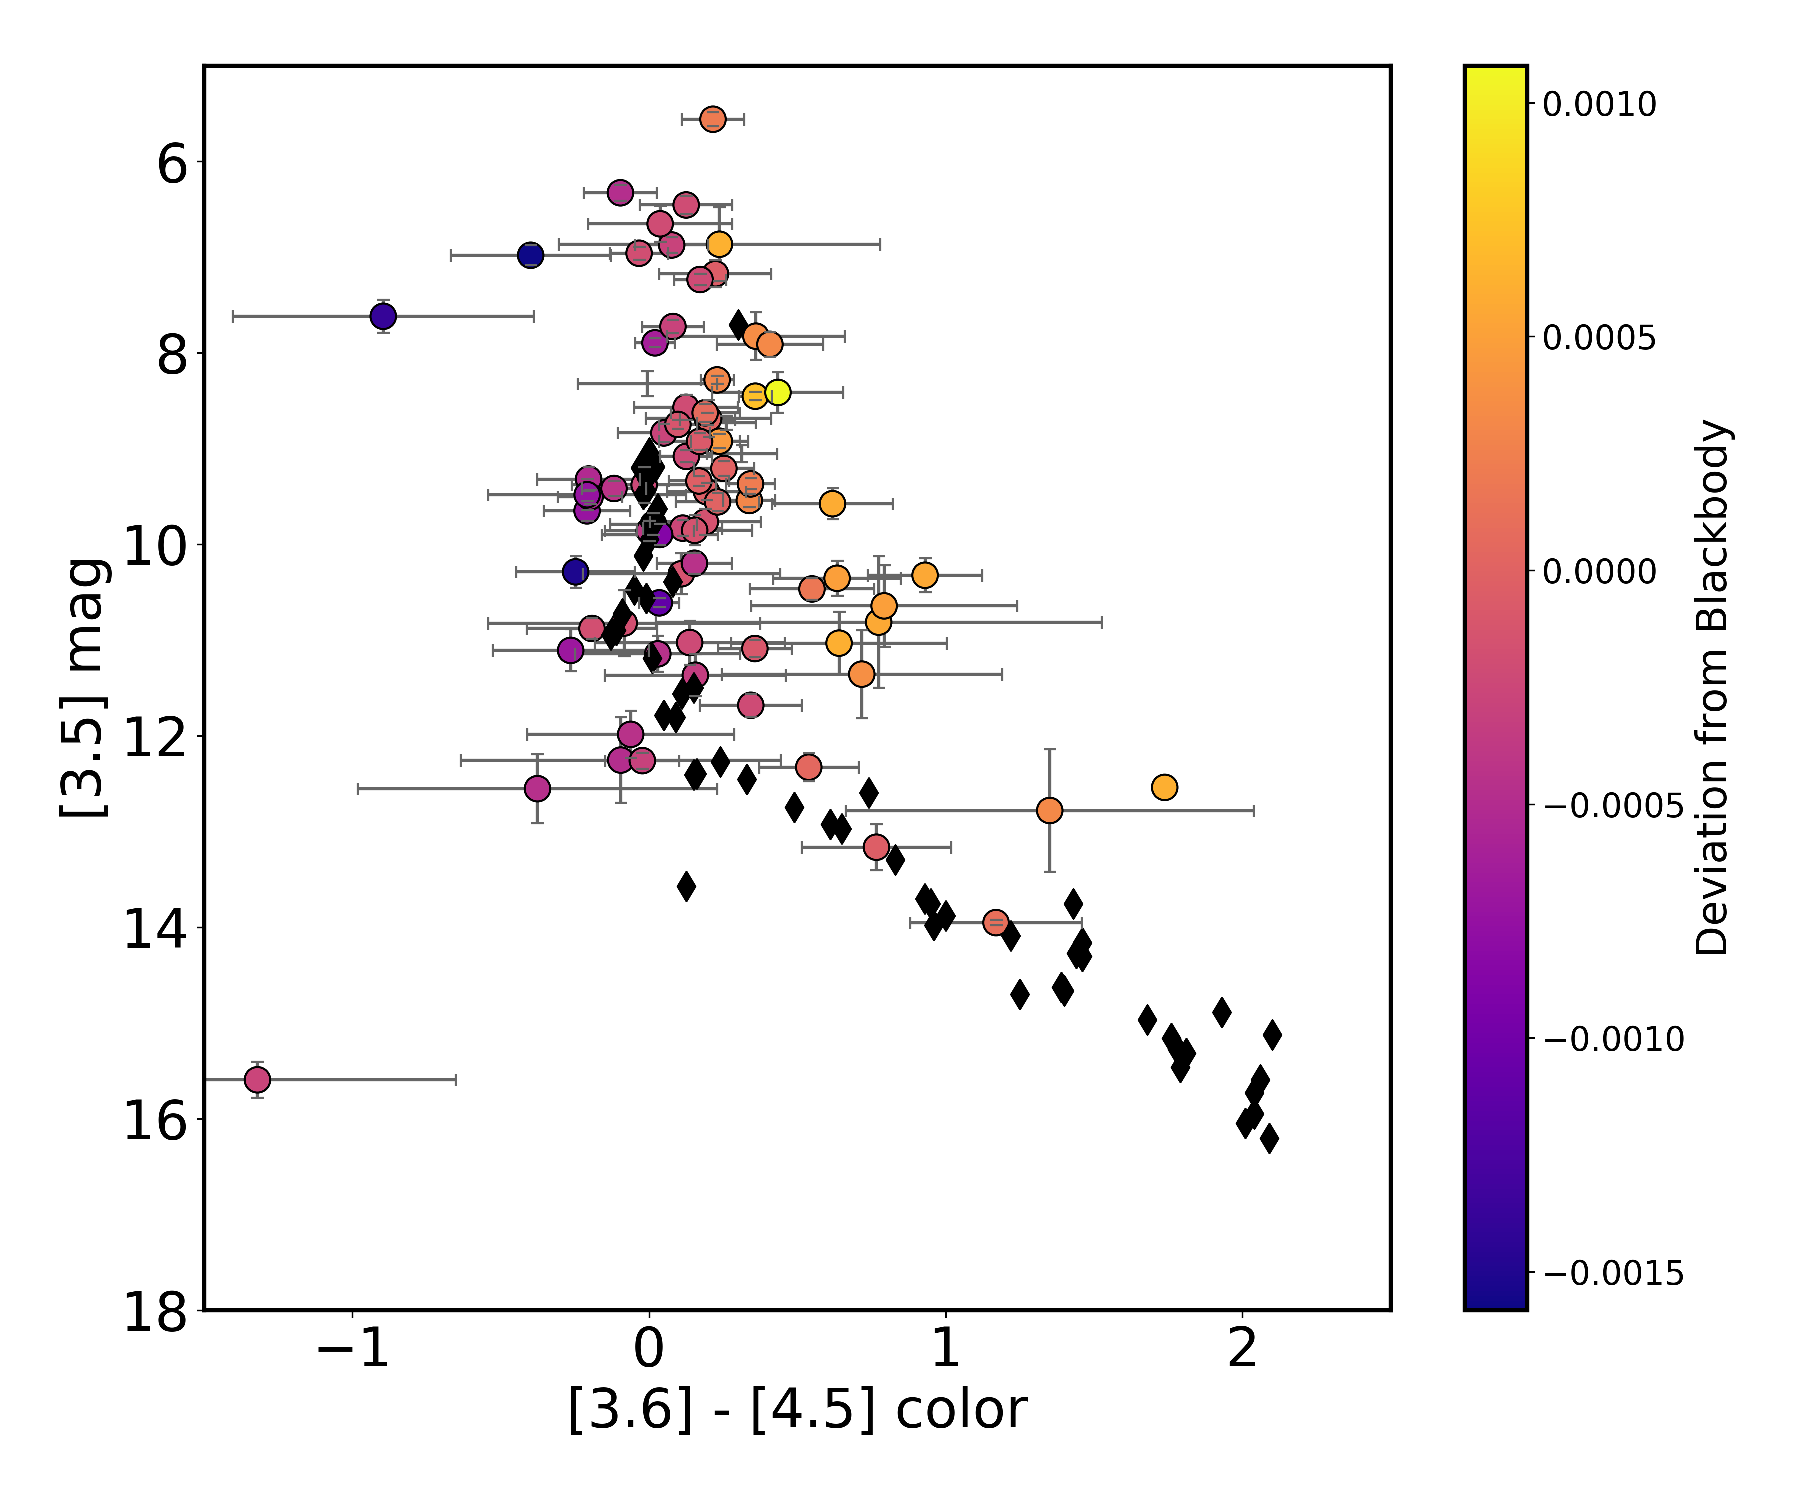
\includegraphics[width = \linewidth]{color+bd+emily.pdf}
    \caption{[3.6] - [4.5] color vs [3.6] magnitude diagram of exoplanets and brown dwarfs planets with available eclipse depth measurements in the two warm \spitzer band-passes. Brown dwarf colors (estimated from the WISE catalog) are shown as black diamonds from \citet{Dupuy2012}. The color scale is the deviation from a blackbody metric described \citet{Baxter2020}.}
    \label{P1:fig:colourmag}
\end{figure}

Figure \ref{P1:fig:colourmag} shows the [3.6] - [4.5] color vs [3.6] magnitude diagram, we have over-plotted the survey of brown dwarfs spanning M, L, and T spectral classes from \citet{Dupuy2012} for comparison. The planets plotted on Figure \ref{P1:fig:colourmag} show an increasing scatter with increasing 3.6~$\mu$m magnitude. This is unlike the brown dwarf spectral sequence which follows the a very tight L/T transition. This increase in scatter confirms the one seen in \citet{Triaud2014c, Beatty2014, Melville2020} and \citet{Dransfield2020}, which is suggested to be due to an increase in atmospheric diversity.

Figure \ref{P1:fig:colourmag} shows that the increase in scatter is driven by a small family of planets which lie redder than the brown dwarf spectral sequence. The color scale shows that this family of planets shows a positive deviation from a blackbody \citep{Baxter2020}. The positive deviation from a blackbody indicates methane absorption (nominal TP profile) or CO emission (inverted TP profile). Since these planets are around 1200-1500~K, we do not expect their atmospheres to be inverted, and we therefore think that these warmer planets could be displaying a signature of methane in their atmospheres. In Section \ref{P1:subsec:TDvsTeq} we show that the cooler planets (<1000~K) deviate from equilibrium chemistry models by not showing signatures of methane in their atmospheres. Similarly, these warmer planets are not expected to have a high methane abundance given equilibrium chemistry, we again have to invoke non-equilibrium processes such as vertical mixing. Warmer planets are expected to have larger vertical mixing than their cooler counterparts \citep{Komacek2019}, creating an ideal scenario for dredging up methane. Furthermore, brown dwarfs are expected to have smaller mixing than gas giant planets, with $K_{zz}$ ranging from $10^4-10^8.5$ for brown dwarfs and $10^7-10^{12}$ \citep{Zahnle2014, Leggett2017, Miles2020}. Although this prediction is based on non-irradiated, higher gravity objects with mostly convective atmospheres, GCMs of highly irradiated, radiative atmospheres of hot Jupiters do display stronger mixing \citep{Parmentier2013, Komacek2019}. We therefore propose that the increased atmospheric diversity of planets compared to their brown dwarf counterparts seen in Figure \ref{P1:fig:colourmag} could be due, in part, to the diversity of processes involved, such as the presence of vertical mixing.

Furthermore, brown dwarfs are expected to have smaller mixing than gas-giant planets \citep{Zahnle2014}. Although this prediction is based on non-irradiated, higher gravity objects with mostly convective atmospheres, GCMs of highly irradiated, essentially radiative atmospheres of hot Jupiters do display stronger mixing \citep{Parmentier2013, Komacek2019}. With $K_{zz}$ ranging from $10^4-10^{8.5}$~\cmcms~for brown dwarfs \citep{Zahnle2014, Leggett2017, Miles2020} and $10^7-10^{12}$~\cmcms~for gas giants \citep{Parmentier2013, Komacek2019}. We therefore propose that the increased atmospheric diversity of planets compared to their brown dwarf counterparts seen in Figure \ref{P1:fig:colourmag} could be due, in part, to the diversity of processes involved, such as the presence of vertical mixing.

\section{Conclusion}
\label{P1:sec:conclusion}

We have performed the data analysis of 70 lightcurves and presented in total 49 planets with transit depths at 3.6 and 4.5~$\mu$m with \textit{Spitzer}/IRAC. This survey represents the largest analysis of \spitzerIRAC observations of gas giant transits to date, and it spans equilibrium temperatures from 500~K to 2700~K. We have implemented our custom \spitzerIRAC data analysis pipeline which thoroughly searches over a grid of data reduction parameters before employing pixel level decorrelation \citep{Deming2015} to correct for the strong \spitzer systematics and extract the transit depths using an MCMC transit fitting algorithm.

We then statistically studied the sample of all planets with transmission in these two bandpasses. We create a fiducial cloud-free 1-D atmospheric model grid with 1x solar composition and equilibrium chemistry spanning the parameters of the planets in our sample. We compare the survey of planets with this model grid and note a family of outliers with equilibrium temperature <1000~K, they do not show the expected methane abundance from these equilibrium chemistry models.

Next, we expand our grid in two dimensions by extending to 30x solar metallicity and incorporating non-equilibrium effects with different values of an eddy diffusion co-efficient ($K_{zz}$). We find that the best fitting grid for the cool planets (T<1000~K) has high metallicity (30x solar) and low or no vertical mixing ($K_{zz}=0$ or $10^8$~\cmcms). On the other hand, we find that the hot planets (T>1000~K) are best explained with 1x solar composition with a marginal better fit with the high vertical mixing model ($K_{zz}=10^{12}$~\cmcms). We conclude that the cool planets are better fit by models with higher metallicity as due to an observational bias resulting in lower masses. We find evidence supporting non-equilibrium chemistry in a survey of planets and find that our work agrees with the theory that hotter planets have higher vertical mixing.

Furthermore, we combine our transits with our previous literature eclipse survey. We do not find any trend between eclipses and transits, and propose that this is due to several effects: clouds at different pressures or more complex atmospheric processes. We then create a color magnitude diagram using the emission observations and compare to L/T transition brown dwarfs. With a larger sample size than previous studies, we also see the increase in scatter with increasing magnitude first seen in \citet{Triaud2014c}. We see that the increase in scatter is driven by a family of mid-temperate planets showing a methane signature, which is not expected from equilibrium chemistry. We propose that this increase in scatter is due to methane being dredged up due to high levels of vertical mixing in the atmosphere. Which supports the theory that brown dwarfs have $\sim$100x lower levels of vertical mixing than planets.

\begin{subappendices}

  \section{Pipeline results Figures and Tables}
  \label{P1:app:piperes}


  \longtab{
  \begin{landscape}
  \setlength{\tabcolsep}{3pt}
  \begin{longtable}{llllllllll}

  \caption[]{\label{P1:tab:jumpParams} Jump Parameters used as starting points for the MCMC analysis. Eccentricity was fixed to 0 for all planets since it did not affect the resulting transit depths. Stellar parameters (Teff, logg and [Fe/H]) are used to calculate linear limb-darkening parameters.} \\

  \hline\hline
  Planet & $a/R_s$ & inc & $R_p/R_s$ & Period &  Eccentricity &        $T_{\rm eff}$ & $log(g_*)$ & [Fe/H] & Ref  \\
   &  & $^{\circ}$ &  & days &   & Kelvin & $\log_{10}(cm/s^2)$ & dex &          \\
  \hline
  \endfirsthead
  \caption{continued.} \\
  \hline\hline
  Planet & $a/R_s$ & inc & $R_p/R_s$ & Period &  Eccentricity &        $T_{\rm eff}$ & $log(g_*)$ & [Fe/H] & Ref  \\
   &  & $^{\circ}$ &  & days &   & Kelvin & $\log_{10}(cm/s^2)$ & dex &          \\
  \hline
  \endhead
  \hline
  \endfoot
  HAT-P-32 b    &   6.05(4) &     88.9(4) &       0.1508(4) &         2.150008(1) &       0.16(6) &   6207(88) &      4.33(1) &  -0.04(8) &                                13          \\
  XO-1 b       &  11.24(9) &    88.8(2) &       0.1320(5) &         3.94150685(91) &    0 &         5750(75) &      4.50(1) &   0.02(8) &                                  6 \\
  HAT-P-1 b     &   9.85(7) &    85.63(06) &     0.1180(2) &         4.46529976(55) &    0 &         5980(49) &      4.36(1) &   0.13(1) &                                19       \\
  WASP-17 b    &   7.05(7) &    86.83(68) &     0.13 &              3.7354380(68) &     0.03(2) &   6650(80) &      4.16(3) &  -0.19(9) &                               1        \\
  WASP-39 b    &  11.37(24) &   87.75(27) &     0.1457(16) &        4.0552765(35) &     0 &         5400(150) &     4.4(2) &   -0.12(10) &                            18,10      \\
  HAT-P-12 b    &  11.77(21) &   89.0(4) &       0.1406(13) &        3.2130598(21) &     0.03(3) &   4650(60) &      4.61(1) &  -0.29(5) &                               11      \\
  HAT-P-18 b    &  16.04(75) &   88.8(3) &       0.1365(15) &        5.508023(6) &       0.08(5) &   4803(80) &      4.57(4) &    0.10(08) &                                14    \\
  TrES2 b     &    7.90(2) &   83.87(02) &     0.1254(5) &         2.47061317(9) &     0.02(2) &   5850(50) &      4.43(2) &   -0.15(10) &                                9, 22   \\
  WASP-4 b     &   5.46(2) &    88.52(39) &     0.1544(2) &         1.33823204(16) &    0.003(7) &  5436(34) &      4.46(5) &  -0.05(4) &                                  15,20    \\
  XO-2 b       &   8.18(3) &    88.9(7) &       0.1 &               2.615857(50) &      0 &         5340(32) &      4.48(5) &   0.45(2) &                                         5  \\
  GJ3470 b    &  13.94(49) &   88.88(72) &     0.0764(4) &         3.3366487(43) &     0.02(2) &   3652(50) &      4.78(12) &   0.17(6) &                                 3        \\
  WASP-21 b    &   9.62(17) &   87.12(24) &     0.1030(8) &         4.3225126(22) &     0 &         5800(100) &     4.2(1) &  -0.46(11) &                               21,4        \\
  WASP-31 b    &    8.00(19) &  84.41(22) &     0.127 &             3.4059096(50) &     0 &         6302(102) &     4.31(2) &   -0.20(09) &                               2       \\
  WASP-1 b     &   5.69(6) &    90.0(1.3) &     0.1036(8) &         2.5199454(5) &      0.01(3) &   6200(200) &     4.3(3) &     0.1(2) &                            17,7       \\
  HAT-P-26 b    &  13.44(83) &   88.6(9) &       0.0737(12) &        4.234516(15) &      0.12(6) &   5079(88) &      4.56(6) &  -0.04(8) &                               12     \\
  WASP-107 b   &    18.2(1) &   89.56(08) &     0.1446(2) &         5.72149242(46) &    0 &         4430(120) &     4.5(1) &    0.02(10) &                                 23 \\
  WASP-13 b    &   7.58(15) &   85.64(24) &     0.0922(8) &         4.353011(13) &      0 &         5826(100) &     4.04(20) &     0.0(2) &                                 24,25    \\
  WASP-121 b   &   3.75(3) &    87.6(6) &       0.1245(5) &         1.27492550(25) &    0 &         6459(140) &     4.24(1) &   0.13(9) &                                 26  \\
  WASP-69 b    &  11.96(17) &   86.71(20) &     0.1336(16) &        3.8681382(17) &     0 &         4700(50) &      4.54(2) &   0.15(8) &                                35    \\
  WASP-67 b    &  13.42(13) &   85.8(3) &       0.1345(48) &        4.61442(1) &        0 &         5417(85) &      4.53(2) &   0.18(6) &                                36       \\
  HATS7 b     &  10.59(51) &   87.92(75) &     0.0711(19) &        3.185315(5) &       0 &         4985(50) &      4.54(5) &   0.25(8) &                               37  \\
  WASP-29 b    &  12.15(44) &   88.8(7) &       0.101(2) &          3.922719(7) &       0.03(5) &   4875(65) &      4.54(4) &   0.11(14) &                                38   \\
  HAT-P-41 b    &   5.45(18) &   87.7(1.0) &     0.1028(16) &        2.694050(4) &       0 &         6390(100) &     4.14(2) &    0.21(10) &                                32\\
  WASP-101 b   &    8.45(30) &  85.0(2) &       0.1140(9) &         3.585720(4) &       0 &         6380(120) &     4.31(8) &    0.20(12) &                                32\\
  WASP-131 b   &   8.53(9) &    85.0(3) &       0.0815(7) &         5.322023(5) &       0 &         6030(90) &      4.09(3) &  -0.18(8) &                                39       \\
  WASP-36 b    &   5.85(6) &    83.15(13) &     0.1368(6) &         1.53736596(24) &    0 &         5959(134) &     4.49(1) &   -0.26(10) &                                40     \\
  WASP-63 b    &    6.59(30) &  87.8(1.3) &     0.0781(11) &        4.378080(6) &       0 &         5550(100) &     4.01(3) &   0.08(7) &                                32\\
  WASP-79 b    &   7.03(36) &   85.4(6) &       0.1049(24) &        3.662380(5) &       0 &         6600(100) &     4.20(15) &    0.03(1)&                                32\\
  WASP-94 Ab   &    7.3(7) &    88.7(7) &       0.1094(8) &         3.9501907(44) &     0 &         6153(75) &      4.18(1) &   0.26(15) &                          41          \\
  WASP-74 b    &    4.86(20) &  79.81(24) &     0.0964(7) &         2.137750(1) &       0 &         5990(110) &     4.39(7) &    0.03(10) &                                33 \\
  WASP-62 b    &   9.55(41) &   88.30(75) &     0.1095(9) &         4.411950(3) &       0 &         6230(80) &      4.45(10) &   0.04(6) &                                34 \\
  Kepler-45 b  &    10.6(1.0) & 87.0(7) &       0.179(2) &          2.455239(4) &       0.11(10) &  3820(90) &      3.1(1) &   0.13(13) &                                16      \\
  \hline
  \end{longtable}
  \tablebib{(1)~\citet{Anderson2011b};
    (2) \citet{Anderson2011a}; (3) \citet{Biddle2014}; (4) \citet{Bouchy2010};
    (5) \citet{Burke2007}; (6) \citet{Burke2010}; (7) \citet{CollierCameron2007};
    (8) \citet{Doyle2011}; (9) \citet{Esteves2015}; (10) \citet{Faedi2011};
    (11) \citet{Hartman2009}; (12) \citet{Hartman2011b}; (13) \citet{Hartman2011c};
    (14) \citet{Hartman2011a}; (15) \citet{Hoyer2013}; (16) \citet{Johnson2012};
    (17) \citet{Maciejewski2014}; (18) \citet{Maciejewski2016}; (19) \citet{Nikolov2014};
    (20) \citet{Petrucci2013}; (21) \citet{Seeliger2015}; (22) \citet{Sozzetti2007};
    (23) \citet{Mocnik2017}; (24) \citet{Barros2012}; (25) \citet{Skillen2009};
    (26) \citet{Delrez2016}; (27) \citet{Holman2010}; (28) \citet{Torres2011};
    (32) \citet{Stassun2017}; (33) \citet{Stassun2018}; (34) \citet{Stassun2019};
    (35) \citet{Anderson2014}; (36) \citet{Hellier2012}; (37) \citet{Bakos2015};
    (38) \citet{Hellier2010}; (39) \citet{Hellier2017}; (40) \citet{Mancini2016};
    (41) \citet{Neveu-VanMalle2014}.}
  \end{landscape}
  }


  \begin{figure*}[!b]
    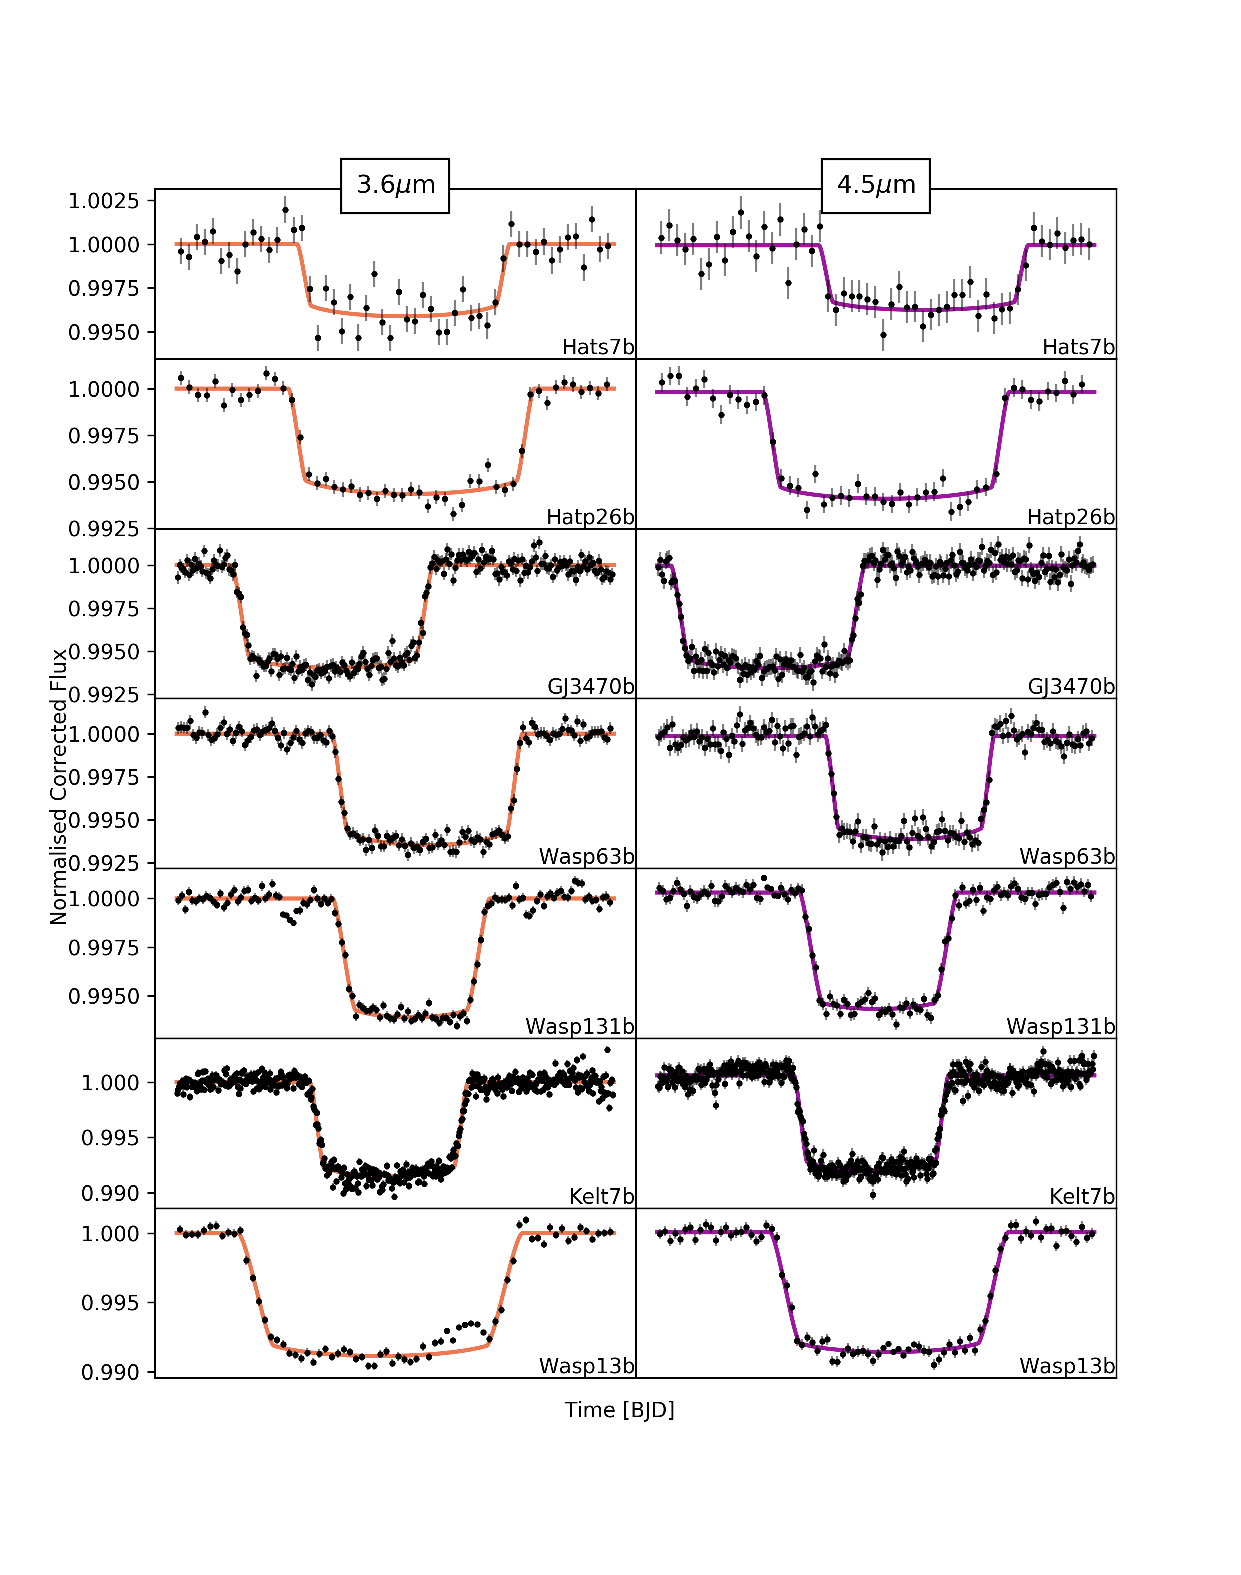
\includegraphics[trim={0 2cm 0 0},clip,width=\textwidth]{CorrectedLighctuves0.pdf}
    \caption{Normalized and systematic corrected transit lightcurves for each planet  at 3.6 (left column, orange) and 4.5~$\mu$m (right column, purple). 1 $\sigma$errorbars are those originally calculated from scaled photon noise. The data and the errorbars are binned in 5 minute intervals for display purposes. Continuous curves show the best fit transit models in each band-pass for comparison. Kepler-45b displays the result of 4 phase folded lightcurves in each channel.}
    \label{P1:fig:normlc}
  \end{figure*}

  \addtocounter{figure}{-1}
  \begin{figure*}
    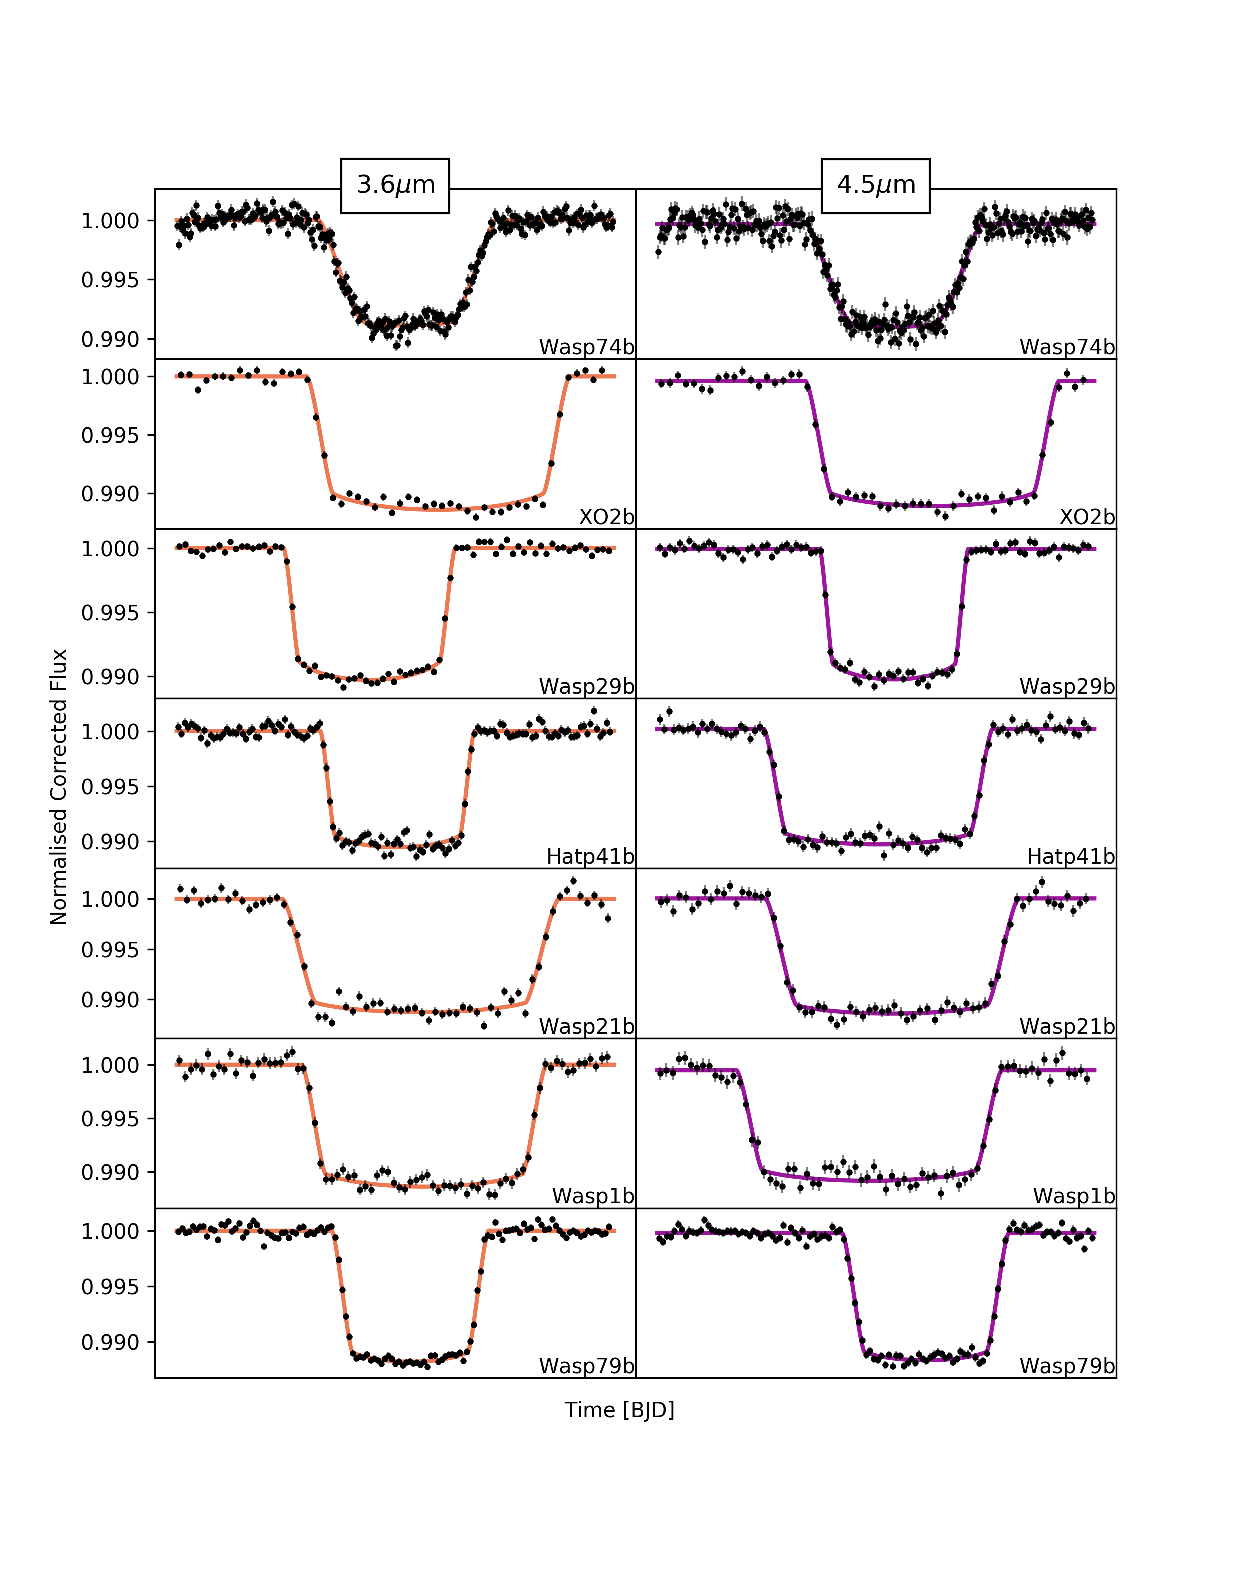
\includegraphics[trim={0 2cm 0 0},clip,width=\textwidth]{CorrectedLighctuves1.pdf}
    \caption{}
    \label{P1:fig:normlc1}
  \end{figure*}

  \addtocounter{figure}{-1}
  \begin{figure*}
    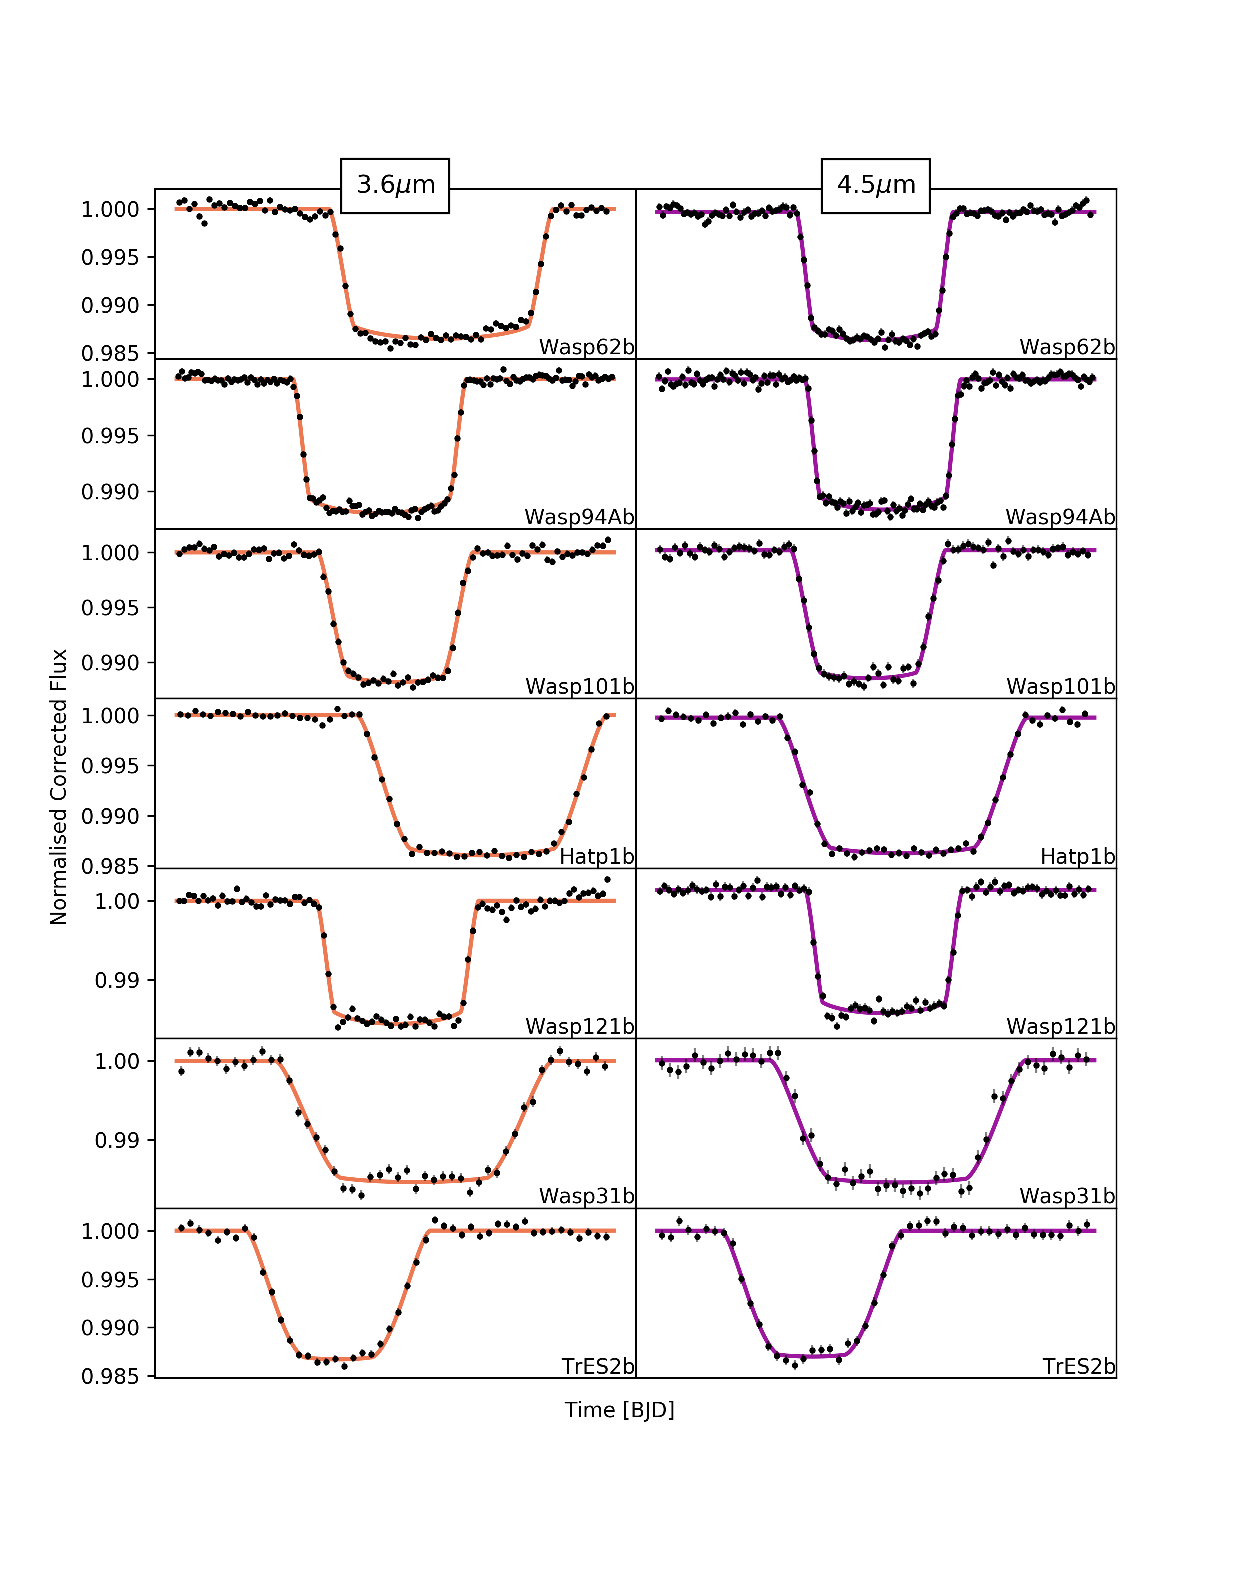
\includegraphics[trim={0 1cm 0 0},clip,width=\textwidth]{CorrectedLighctuves2.pdf}
    \caption{\textit{Continued.}}
    \label{P1:fig:normlc2}
  \end{figure*}

  \addtocounter{figure}{-1}
  \begin{figure*}
    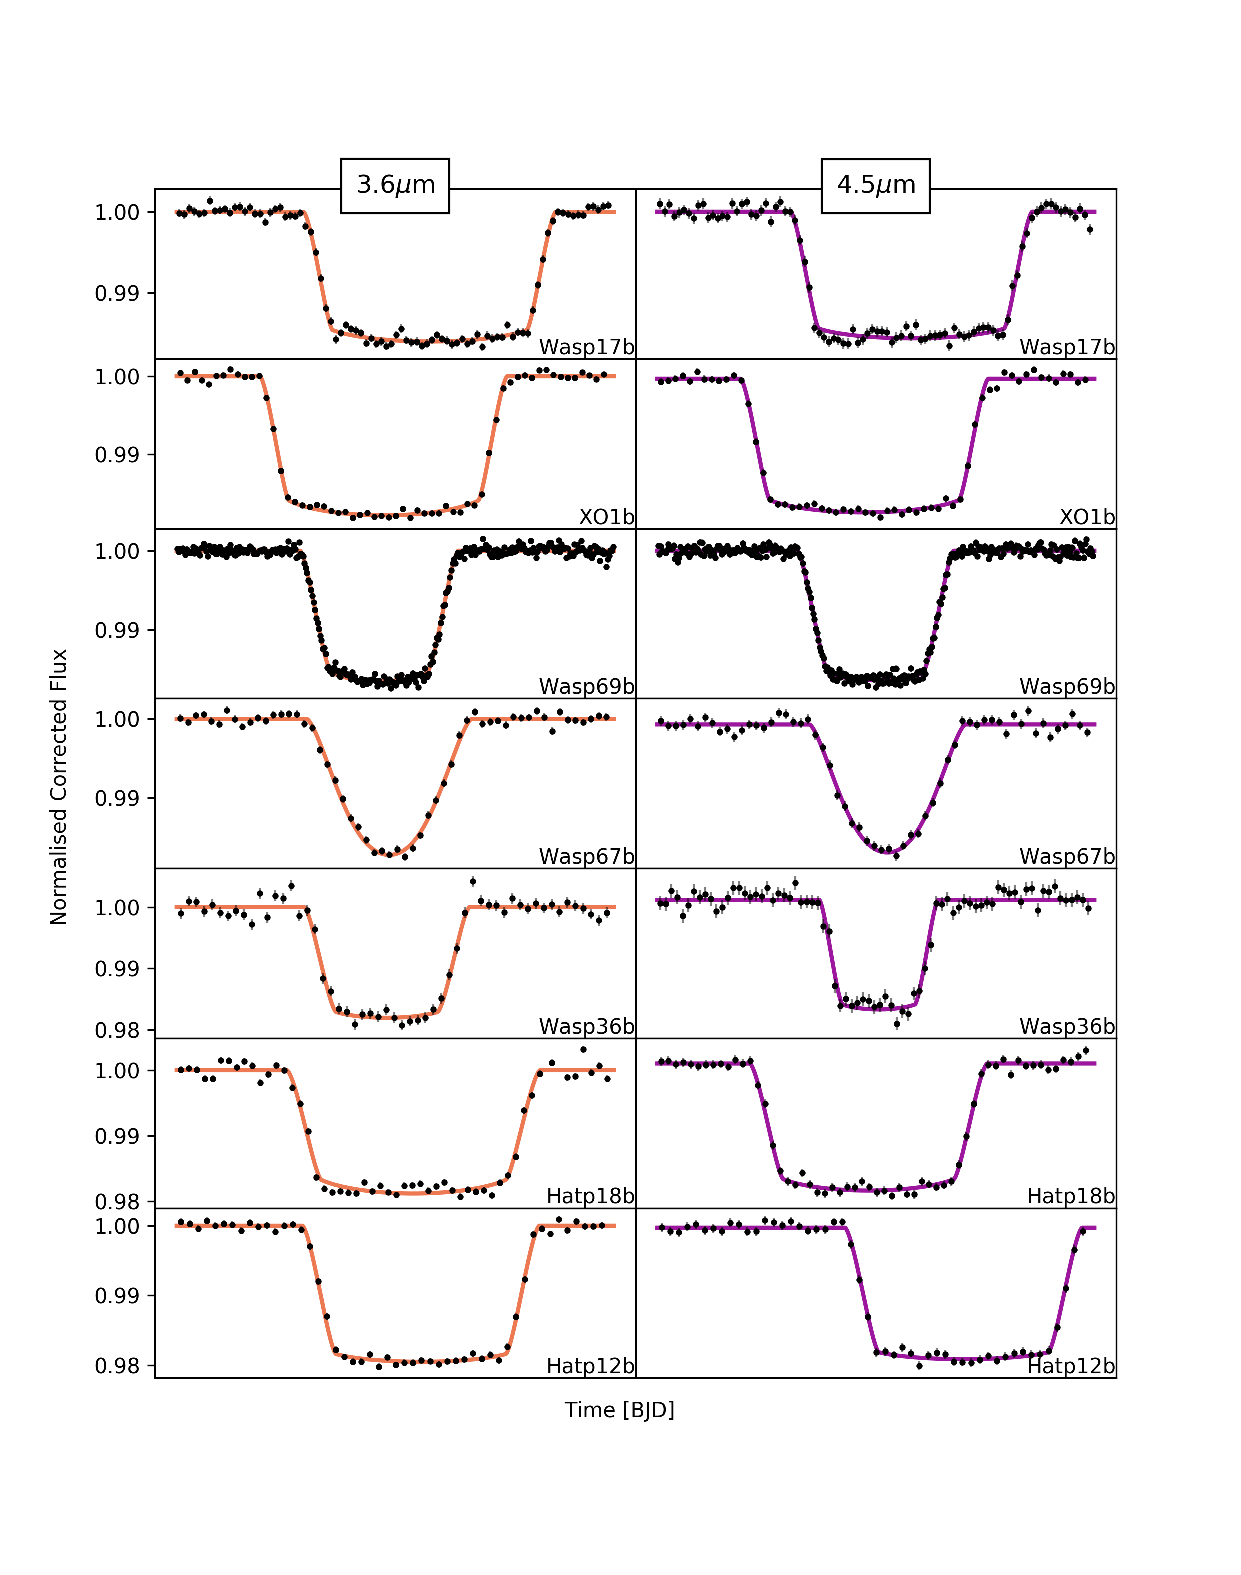
\includegraphics[trim={0 1cm 0 0},clip,width=\textwidth]{CorrectedLighctuves3.pdf}
    \caption{\textit{Continued.}}
    \label{P1:fig:normlc3}
  \end{figure*}

  \addtocounter{figure}{-1}
  \begin{figure*}
    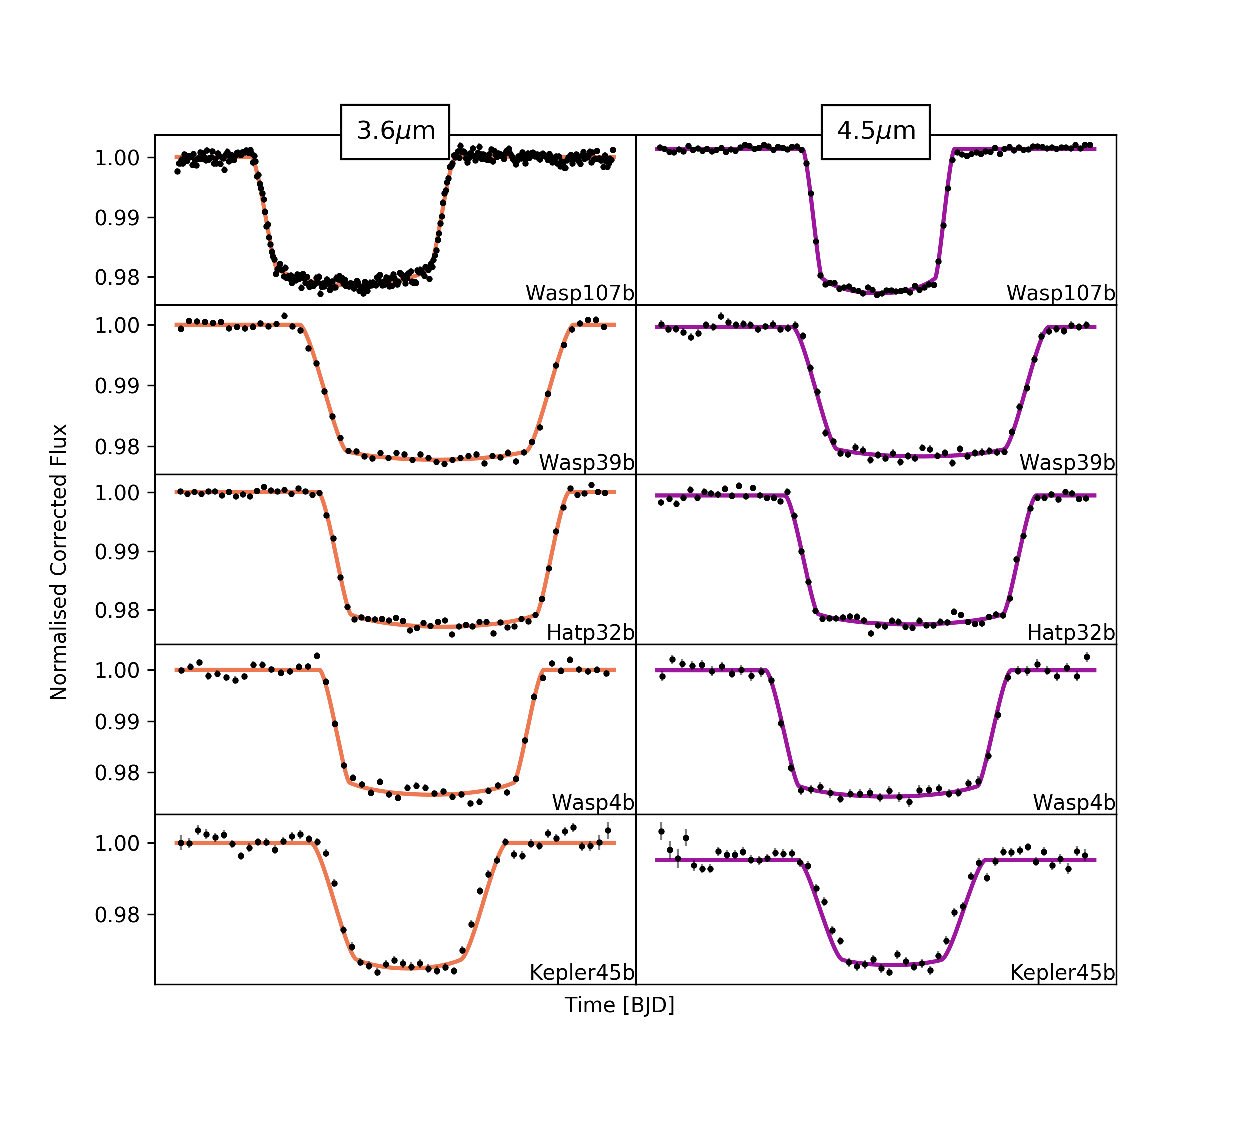
\includegraphics[trim={0 1cm 0 0},clip,width=\textwidth]{CorrectedLighctuves4.pdf}
    \caption{\textit{Continued.}}
    \label{P1:fig:normlc4}
    \end{figure*}



  \longtab{
  \begin{landscape}
  \setlength{\tabcolsep}{2pt}
  \begin{longtable}{llllllllllc}

  \caption{\label{P1:tab:eclipses} Eclipse depths at 3.6 and 4.5$\mu$m collected from the literature ( $(F_p/F_s)_{3.6}$ and $(F_p/F_s)_{4.5}$ respectively). $T_{eq}$ is the equilibrium temperature assuming no redistribution and 0 albedo, Distance is the estimated distance in parsec taken from \citet{Bailer-Jones2018}. $m_{W1}^{s}$ and $m_{W2}^{s}$ are the stellar apparent  magnitudes. $M_{3.6}^{pl}$ and $M_{4.5}^{pl}$ and the planetary absolute magnitudes in the wise 1 and wise 2 bandpasses (which are equivalent to the \spitzer channel 1 and channel 2 respectively), calculated using the planet to star flux ratio. Color is the 4.5 minus 3.6 micron magnitude color of the planets. The final column details the reference for each of the eclipse depths in the literature, the majority of which were collected from exoplanets.org \citep{Wright2011} and have been individually verified.} \\

  \hline\hline
  Planet & $(F_p/F_s)_{3.6}$ & $(F_p/F_s)_{4.5}$ & $T_{eq}$ (a=0) &  Distance  & $M_{3.6}^{pl}$ &    $M_{4.5}^{pl}$ &  $m_{W1}^{s}$ &  $m_{W2}^{s}$ &         color  &  Ref.
  & ppm & ppm & Kelvin & parsec & mag & mag & mag & mag & mag &  \\
  \hline
  \endfirsthead
  \caption{continued.} \\
  \hline\hline
  Planet & $(F_p/F_s)_{3.6}$ & $(F_p/F_s)_{4.5}$ & $T_{eq}$ (a=0) &  Distance  & $M_{3.6}^{pl}$ &    $M_{4.5}^{pl}$ &  $m_{W1}^{s}$ &  $m_{W2}^{s}$ &         color  &  Ref. \\
  & ppm & ppm & Kelvin & parsec & mag & mag & mag & mag & mag &  \\
  \hline
  \endhead
  \hline
  \endfoot
  HAT-P-32 b     &    3640$\pm$160 &    4380$\pm$200 &   1901$\pm$57 &    289.2$\pm$5.3 &   8.7$\pm$0.1 &    8.5$\pm$0.07 &    9.9$\pm$0.02 &   9.91$\pm$0.02 &    0.2$\pm$0.09 &        1 \\
  XO-1 b        &      860$\pm$70 &     1220$\pm$90 &   1207$\pm$30 &    163.6$\pm$0.6 &  11.1$\pm$0.1 &  10.73$\pm$0.08 &   9.49$\pm$0.02 &   9.52$\pm$0.02 &   0.36$\pm$0.12 &        2 \\
  HAT-P-1 b      &      800$\pm$80 &    1350$\pm$220 &   1306$\pm$33 &    159.0$\pm$1.0 &  10.5$\pm$0.1 &   9.92$\pm$0.18 &   8.73$\pm$0.02 &   8.75$\pm$0.02 &   0.55$\pm$0.21 &        3 \\
  WASP-39 b     &     880$\pm$150 &     960$\pm$180 &   1118$\pm$35 &    214.0$\pm$1.7 &  11.1$\pm$0.2 &  11.12$\pm$0.21 &  10.16$\pm$0.02 &  10.22$\pm$0.02 &   0.03$\pm$0.28 &        4 \\
  HAT-P-12 b     &     660$\pm$270 &     640$\pm$180 &    958$\pm$18 &    142.8$\pm$0.5 &  12.3$\pm$0.4 &  12.35$\pm$0.31 &  10.08$\pm$0.02 &  10.14$\pm$0.02 &   -0.1$\pm$0.54 &        5 \\
  HAT-P-18 b     &     437$\pm$145 &     326$\pm$146 &    847$\pm$26 &    161.4$\pm$0.6 &  12.6$\pm$0.4 &  12.93$\pm$0.49 &   10.2$\pm$0.02 &  10.25$\pm$0.02 &  -0.38$\pm$0.61 &        6 \\
  TrES2 b      &    1270$\pm$210 &    2300$\pm$240 &   1498$\pm$32 &    215.3$\pm$1.0 &  10.4$\pm$0.2 &   9.72$\pm$0.12 &   9.78$\pm$0.02 &   9.79$\pm$0.02 &   0.63$\pm$0.21 &        7 \\
  WASP-4 b      &    3190$\pm$310 &    3430$\pm$270 &   1651$\pm$27 &    267.2$\pm$3.7 &   9.8$\pm$0.1 &   9.78$\pm$0.09 &  10.68$\pm$0.02 &  10.75$\pm$0.02 &   0.01$\pm$0.15 &        8 \\
  XO-2 b        &     810$\pm$170 &     980$\pm$200 &   1322$\pm$23 &    154.3$\pm$1.4 &  11.0$\pm$0.2 &  10.89$\pm$0.22 &   9.24$\pm$0.02 &   9.31$\pm$0.02 &   0.14$\pm$0.32 &        9 \\
  GJ3470 b     &      113$\pm$24 &        3$\pm$22 &    662$\pm$45 &     29.4$\pm$0.1 &  15.3$\pm$0.2 &  19.25$\pm$7.96 &   7.81$\pm$0.03 &   7.78$\pm$0.02 &  -3.92$\pm$7.97 &       10 \\
  WASP-1 b      &    1170$\pm$160 &    2120$\pm$210 &   1876$\pm$69 &   393.1$\pm$10.5 &   9.6$\pm$0.2 &   8.96$\pm$0.12 &  10.22$\pm$0.02 &  10.25$\pm$0.02 &    0.62$\pm$0.2 &       11 \\
  HAT-P-26 b     &        85$\pm$0 &      265$\pm$70 &    994$\pm$48 &    141.8$\pm$1.1 &  14.0$\pm$0.0 &  12.78$\pm$0.29 &   9.54$\pm$0.02 &    9.6$\pm$0.02 &   1.17$\pm$0.29 &        6 \\
  WASP-121 b    &    3685$\pm$114 &    4684$\pm$121 &   2359$\pm$61 &    269.9$\pm$1.6 &   8.3$\pm$0.0 &   8.05$\pm$0.04 &   9.36$\pm$0.02 &   9.39$\pm$0.02 &   0.23$\pm$0.06 &       12 \\
  WASP-87 b     &    2080$\pm$127 &    2708$\pm$137 &   2343$\pm$68 &    298.4$\pm$3.6 &   8.7$\pm$0.1 &   8.47$\pm$0.06 &    9.4$\pm$0.02 &   9.43$\pm$0.02 &    0.26$\pm$0.1 &       12 \\
  WASP-100 b    &     1267$\pm$98 &    1720$\pm$119 &  2200$\pm$171 &    364.4$\pm$2.7 &   9.1$\pm$0.1 &   8.74$\pm$0.08 &   9.62$\pm$0.02 &   9.64$\pm$0.02 &   0.31$\pm$0.12 &       12 \\
  WASP-78 b     &    2001$\pm$218 &    2013$\pm$351 &  1957$\pm$256 &   754.3$\pm$16.7 &   8.3$\pm$0.1 &    8.33$\pm$0.2 &  10.96$\pm$0.02 &  10.98$\pm$0.02 &  -0.01$\pm$0.24 &       12 \\
  HAT-P-41 b     &    1842$\pm$319 &    2303$\pm$177 &   1937$\pm$44 &    348.2$\pm$4.5 &   8.7$\pm$0.2 &   8.49$\pm$0.09 &   9.56$\pm$0.02 &    9.6$\pm$0.02 &    0.2$\pm$0.21 &       12 \\
  WASP-101 b    &    1161$\pm$111 &    1194$\pm$113 &   1554$\pm$40 &    201.2$\pm$1.1 &   9.9$\pm$0.1 &   9.86$\pm$0.11 &   9.04$\pm$0.02 &   9.07$\pm$0.02 &    0.0$\pm$0.15 &       12 \\
  WASP-131 b    &      304$\pm$96 &      289$\pm$80 &   1458$\pm$35 &    200.1$\pm$2.6 &  10.8$\pm$0.3 &   10.91$\pm$0.3 &   8.54$\pm$0.02 &   8.57$\pm$0.02 &  -0.08$\pm$0.46 &       12 \\
  WASP-36 b     &     914$\pm$578 &    1953$\pm$544 &   1722$\pm$45 &    386.3$\pm$5.2 &  10.8$\pm$0.7 &   10.04$\pm$0.3 &  11.15$\pm$0.02 &   11.2$\pm$0.02 &   0.77$\pm$0.75 &       12 \\
  WASP-63 b     &      486$\pm$96 &     560$\pm$130 &   1531$\pm$45 &    290.7$\pm$2.0 &  10.3$\pm$0.2 &   10.2$\pm$0.25 &   9.34$\pm$0.02 &   9.39$\pm$0.02 &   0.11$\pm$0.33 &       12 \\
  WASP-94 A b    &      867$\pm$59 &      995$\pm$93 &   1500$\pm$76 &    211.2$\pm$2.5 &   9.8$\pm$0.1 &   9.72$\pm$0.11 &    8.8$\pm$0.02 &   8.84$\pm$0.02 &   0.11$\pm$0.13 &       12 \\
  WASP-62 b     &    1616$\pm$146 &    1359$\pm$130 &   1427$\pm$35 &    175.6$\pm$0.6 &   9.7$\pm$0.1 &   9.86$\pm$0.11 &    8.9$\pm$0.02 &   8.92$\pm$0.02 &  -0.21$\pm$0.15 &       12 \\
  CoRoT-1 b   &    4150$\pm$420 &    4820$\pm$420 &   1900$\pm$81 &   787.9$\pm$23.5 &   8.6$\pm$0.1 &   8.45$\pm$0.12 &   12.1$\pm$0.02 &  12.14$\pm$0.02 &   0.12$\pm$0.17 &       13 \\
  CoRoT-2 b   &    3550$\pm$200 &    5000$\pm$200 &   1537$\pm$40 &    213.3$\pm$2.5 &   9.5$\pm$0.1 &   9.21$\pm$0.05 &  10.06$\pm$0.02 &   10.1$\pm$0.02 &   0.34$\pm$0.09 &       13 \\
  GJ 436 b    &      155$\pm$22 &       34$\pm$20 &    649$\pm$59 &      9.8$\pm$0.0 &  15.6$\pm$0.2 &  16.92$\pm$0.64 &   6.02$\pm$0.11 &   5.69$\pm$0.05 &  -1.32$\pm$0.67 &       14 \\
  HAT-P-19 b  &     620$\pm$140 &     620$\pm$140 &   1009$\pm$40 &    202.1$\pm$1.5 &  12.0$\pm$0.2 &  12.05$\pm$0.25 &   10.5$\pm$0.02 &  10.56$\pm$0.02 &  -0.06$\pm$0.35 &        4 \\
  HAT-P-2 b   &      996$\pm$72 &     1031$\pm$61 &   1540$\pm$30 &    127.8$\pm$0.4 &   9.5$\pm$0.1 &   9.52$\pm$0.07 &   7.57$\pm$0.02 &   7.58$\pm$0.02 &   0.03$\pm$0.11 &       15 \\
  HAT-P-20 b  &      615$\pm$82 &     1096$\pm$77 &    971$\pm$24 &     71.0$\pm$0.2 &  12.3$\pm$0.1 &  11.79$\pm$0.08 &   8.56$\pm$0.03 &   8.65$\pm$0.02 &   0.54$\pm$0.17 &       16 \\
  HAT-P-23 b  &    2480$\pm$190 &    3090$\pm$260 &   2051$\pm$71 &    364.8$\pm$4.7 &   9.5$\pm$0.1 &    9.26$\pm$0.1 &  10.75$\pm$0.02 &  10.79$\pm$0.02 &   0.19$\pm$0.13 &       17 \\
  HAT-P-26 b  &      -27$\pm$50 &      223$\pm$81 &    994$\pm$48 &    141.8$\pm$1.1 &   -$\pm$2.0 &   12.97$\pm$0.4 &   9.54$\pm$0.02 &    9.6$\pm$0.02 &    -$\pm$2.05 &        6 \\
  HAT-P-3 b   &    1120$\pm$225 &     940$\pm$125 &   1158$\pm$34 &    134.6$\pm$0.5 &  11.1$\pm$0.2 &  11.37$\pm$0.15 &   9.38$\pm$0.02 &   9.45$\pm$0.02 &  -0.26$\pm$0.26 &        5 \\
  HAT-P-4 b   &    1420$\pm$160 &    1220$\pm$130 &   1694$\pm$47 &    320.5$\pm$2.8 &   9.3$\pm$0.1 &   9.52$\pm$0.12 &   9.73$\pm$0.02 &   9.77$\pm$0.02 &   -0.2$\pm$0.17 &        5 \\
  HAT-P-6 b   &     1170$\pm$80 &     1060$\pm$60 &   1673$\pm$42 &    275.4$\pm$3.6 &   9.4$\pm$0.1 &   9.54$\pm$0.07 &   9.29$\pm$0.02 &    9.3$\pm$0.02 &  -0.12$\pm$0.11 &       18 \\
  HAT-P-7 b   &    1560$\pm$130 &    1900$\pm$110 &   2225$\pm$41 &    341.1$\pm$2.4 &   8.6$\pm$0.1 &   8.44$\pm$0.07 &   9.28$\pm$0.02 &    9.3$\pm$0.02 &   0.19$\pm$0.12 &       19 \\
  HAT-P-8 b   &     1310$\pm$85 &     1110$\pm$75 &   1772$\pm$48 &    211.6$\pm$1.7 &   9.5$\pm$0.1 &   9.71$\pm$0.08 &   8.93$\pm$0.02 &   8.95$\pm$0.02 &   -0.2$\pm$0.11 &       18 \\
  HD 149026 b &      400$\pm$30 &      340$\pm$60 &   1673$\pm$65 &     75.9$\pm$0.2 &  10.9$\pm$0.1 &  11.07$\pm$0.19 &   6.79$\pm$0.07 &    6.8$\pm$0.02 &  -0.19$\pm$0.22 &       20 \\
  HD 189733 b &    2560$\pm$140 &    2140$\pm$200 &   1200$\pm$22 &     19.8$\pm$0.0 &  10.3$\pm$0.2 &  10.54$\pm$0.11 &   5.29$\pm$0.15 &   5.34$\pm$0.05 &   -0.25$\pm$0.2 &       21 \\
  HD 209458 b &     1190$\pm$70 &     1230$\pm$60 &   1446$\pm$19 &     48.3$\pm$0.1 &  10.2$\pm$0.1 &  10.05$\pm$0.06 &   6.31$\pm$0.09 &   6.19$\pm$0.03 &   0.15$\pm$0.13 &       22 \\
  Kepler-12 b &    1370$\pm$200 &    1160$\pm$310 &   1481$\pm$31 &    881.4$\pm$9.7 &   9.5$\pm$0.2 &   9.69$\pm$0.29 &  12.05$\pm$0.02 &  12.08$\pm$0.02 &  -0.21$\pm$0.33 &       23 \\
  Kepler-17 b &    2500$\pm$300 &    3100$\pm$350 &   1745$\pm$39 &   720.8$\pm$10.3 &   9.8$\pm$0.1 &   9.58$\pm$0.13 &  12.55$\pm$0.02 &  12.59$\pm$0.02 &   0.19$\pm$0.19 &       24 \\
  Kepler-5 b  &    1030$\pm$170 &    1070$\pm$150 &   1807$\pm$35 &   899.8$\pm$16.5 &   9.4$\pm$0.2 &    9.4$\pm$0.16 &  11.68$\pm$0.02 &  11.74$\pm$0.02 &  -0.02$\pm$0.24 &       26 \\
  Kepler-6 b  &     690$\pm$270 &    1510$\pm$190 &   1504$\pm$21 &    587.0$\pm$5.0 &  10.6$\pm$0.4 &   9.85$\pm$0.14 &  11.58$\pm$0.02 &  11.64$\pm$0.02 &   0.79$\pm$0.45 &       26 \\
  KOI-13 b    &    1560$\pm$310 &    2220$\pm$230 &   2607$\pm$94 &   519.1$\pm$29.1 &   7.8$\pm$0.2 &   7.47$\pm$0.17 &   9.39$\pm$0.02 &   9.41$\pm$0.02 &    0.36$\pm$0.3 &       27 \\
  Qatar-1 b   &    1511$\pm$455 &    2907$\pm$415 &   1389$\pm$43 &    185.6$\pm$0.8 &  11.0$\pm$0.3 &  10.39$\pm$0.16 &  10.32$\pm$0.02 &   10.4$\pm$0.02 &   0.64$\pm$0.36 &       28 \\
  TrES-3 b    &    3460$\pm$350 &    3720$\pm$540 &   1629$\pm$32 &    231.3$\pm$1.3 &   9.9$\pm$0.1 &   9.86$\pm$0.16 &  10.57$\pm$0.02 &  10.61$\pm$0.02 &    0.04$\pm$0.2 &       29 \\
  TrES-4 b    &    1370$\pm$110 &    1480$\pm$160 &   1785$\pm$41 &    516.0$\pm$6.9 &   8.8$\pm$0.1 &   8.79$\pm$0.12 &  10.24$\pm$0.02 &  10.28$\pm$0.02 &   0.05$\pm$0.15 &       30 \\
  WASP-10 b   &    1000$\pm$110 &    1460$\pm$160 &    960$\pm$24 &    141.0$\pm$0.7 &  11.7$\pm$0.1 &  11.34$\pm$0.12 &   9.93$\pm$0.02 &   10.0$\pm$0.02 &   0.34$\pm$0.17 &        4 \\
  WASP-103 b  &    4458$\pm$383 &    5686$\pm$138 &   2505$\pm$78 &  883.3$\pm$153.1 &   6.9$\pm$0.4 &   6.63$\pm$0.38 &  10.72$\pm$0.02 &  10.75$\pm$0.02 &   0.24$\pm$0.54 &       31 \\
  WASP-12 b   &    4210$\pm$110 &    4280$\pm$120 &   2584$\pm$91 &    427.2$\pm$6.0 &   7.9$\pm$0.0 &   7.88$\pm$0.05 &  10.11$\pm$0.02 &  10.11$\pm$0.02 &   0.02$\pm$0.07 &       32 \\
  WASP-121 b  &    3150$\pm$103 &    4510$\pm$107 &   2359$\pm$61 &    269.9$\pm$1.6 &   8.5$\pm$0.0 &    8.1$\pm$0.03 &   9.36$\pm$0.02 &   9.39$\pm$0.02 &   0.36$\pm$0.06 &       12 \\
  WASP-14 b   &     1870$\pm$70 &    2240$\pm$180 &   1864$\pm$60 &    162.0$\pm$0.8 &   9.3$\pm$0.0 &   9.17$\pm$0.09 &   8.57$\pm$0.02 &    8.6$\pm$0.02 &    0.17$\pm$0.1 &       33 \\
  WASP-18 b   &    3000$\pm$200 &    3900$\pm$200 &   2398$\pm$73 &    123.5$\pm$0.4 &   8.9$\pm$0.1 &   8.69$\pm$0.06 &   8.07$\pm$0.02 &   8.12$\pm$0.02 &    0.24$\pm$0.1 &       34 \\
  WASP-19 b   &    4830$\pm$250 &    5720$\pm$300 &   2066$\pm$46 &    268.3$\pm$1.7 &   9.1$\pm$0.1 &   8.96$\pm$0.06 &  10.44$\pm$0.02 &  10.49$\pm$0.02 &   0.13$\pm$0.09 &       35 \\
  WASP-2 b    &     830$\pm$350 &    1690$\pm$170 &   1300$\pm$71 &    153.2$\pm$1.6 &  11.4$\pm$0.5 &  10.64$\pm$0.11 &   9.58$\pm$0.02 &   9.64$\pm$0.02 &   0.72$\pm$0.47 &       11 \\
  WASP-24 b   &    1590$\pm$130 &    2020$\pm$180 &   1769$\pm$39 &    322.1$\pm$4.4 &   9.6$\pm$0.1 &    9.33$\pm$0.1 &   10.1$\pm$0.02 &  10.13$\pm$0.02 &   0.23$\pm$0.14 &       36 \\
  WASP-33 b   &    2600$\pm$500 &    4100$\pm$200 &   2694$\pm$53 &    121.9$\pm$1.0 &   8.4$\pm$0.2 &   7.98$\pm$0.06 &   7.38$\pm$0.04 &   7.44$\pm$0.02 &   0.43$\pm$0.22 &       37 \\
  WASP-43 b   &    3460$\pm$130 &    3820$\pm$150 &   1375$\pm$79 &     86.7$\pm$0.3 &  10.6$\pm$0.0 &  10.58$\pm$0.05 &   9.15$\pm$0.02 &   9.22$\pm$0.02 &   0.03$\pm$0.07 &       38 \\
  WASP-48 b   &    1760$\pm$130 &    2140$\pm$200 &   2033$\pm$68 &    454.1$\pm$4.4 &   8.9$\pm$0.1 &   8.76$\pm$0.11 &  10.33$\pm$0.02 &  10.37$\pm$0.02 &   0.17$\pm$0.14 &       17 \\
  WASP-5 b    &    1970$\pm$280 &    2370$\pm$240 &   1742$\pm$68 &    309.1$\pm$3.4 &   9.9$\pm$0.2 &    9.7$\pm$0.11 &  10.54$\pm$0.02 &  10.59$\pm$0.02 &   0.15$\pm$0.19 &       39 \\
  WASP-6 b    &     940$\pm$190 &    1150$\pm$220 &   1184$\pm$32 &    197.1$\pm$1.6 &  11.4$\pm$0.2 &  11.21$\pm$0.21 &  10.28$\pm$0.02 &  10.34$\pm$0.02 &    0.16$\pm$0.3 &        4 \\
  WASP-67 b   &     220$\pm$130 &     800$\pm$180 &   1028$\pm$32 &    189.5$\pm$1.5 &  12.8$\pm$0.6 &  11.43$\pm$0.25 &  10.03$\pm$0.02 &  10.08$\pm$0.02 &   1.35$\pm$0.69 &        4 \\
  WASP-69 b   &      421$\pm$29 &      463$\pm$39 &    961$\pm$21 &     50.0$\pm$0.1 &  12.3$\pm$0.1 &  12.28$\pm$0.09 &   7.32$\pm$0.04 &   7.44$\pm$0.02 &  -0.02$\pm$0.13 &        6 \\
  WASP-8 b    &    1130$\pm$180 &      690$\pm$70 &    927$\pm$27 &     90.0$\pm$0.4 &  10.5$\pm$0.2 &  11.05$\pm$0.11 &   7.91$\pm$0.02 &   7.92$\pm$0.02 &  -0.55$\pm$0.21 &       40 \\
  WASP-80 b   &     455$\pm$100 &      944$\pm$65 &    775$\pm$25 &     49.8$\pm$0.1 &  13.2$\pm$0.2 &   12.4$\pm$0.08 &    8.3$\pm$0.02 &   8.32$\pm$0.02 &   0.77$\pm$0.25 &       41 \\
  XO-3 b      &     1010$\pm$40 &     1580$\pm$36 &   2046$\pm$40 &    213.1$\pm$2.7 &   9.6$\pm$0.1 &   9.13$\pm$0.04 &   8.75$\pm$0.02 &   8.76$\pm$0.02 &   0.47$\pm$0.07 &       42 \\
  XO-4 b      &      560$\pm$90 &     1350$\pm$85 &   1639$\pm$35 &    272.7$\pm$2.9 &  10.3$\pm$0.2 &   9.39$\pm$0.08 &   9.37$\pm$0.02 &    9.4$\pm$0.02 &   0.93$\pm$0.19 &       18 \\
  HAT-P-13 b  &     851$\pm$107 &    1090$\pm$124 &   1648$\pm$53 &    246.8$\pm$2.2 &   7.2$\pm$0.1 &   6.95$\pm$0.13 &   8.96$\pm$0.02 &   9.01$\pm$0.02 &   0.22$\pm$0.19 &       12 \\
  HAT-P-30 b  &    1603$\pm$107 &    1783$\pm$147 &   1637$\pm$43 &    214.0$\pm$2.2 &   6.9$\pm$0.1 &    6.8$\pm$0.09 &   9.04$\pm$0.02 &   9.08$\pm$0.02 &   0.08$\pm$0.12 &       12 \\
  HAT-P-33 b  &    1663$\pm$127 &    1896$\pm$199 &   1780$\pm$34 &    396.1$\pm$7.5 &   6.5$\pm$0.1 &   6.33$\pm$0.12 &   10.0$\pm$0.02 &  10.02$\pm$0.02 &   0.13$\pm$0.16 &       12 \\
  HAT-P-40 b  &     988$\pm$168 &    1057$\pm$145 &   1765$\pm$66 &    464.5$\pm$6.4 &   6.7$\pm$0.2 &   6.62$\pm$0.15 &   9.98$\pm$0.02 &  10.01$\pm$0.02 &   0.04$\pm$0.24 &       12 \\
  KELT-2 A b  &      739$\pm$38 &      761$\pm$47 &   1710$\pm$31 &    134.1$\pm$0.8 &   7.0$\pm$0.1 &   6.99$\pm$0.07 &   7.27$\pm$0.04 &   7.34$\pm$0.02 &   -0.03$\pm$0.1 &       12 \\
  KELT-3 b    &     1788$\pm$97 &    1677$\pm$104 &   1822$\pm$44 &    210.3$\pm$5.4 &   6.3$\pm$0.1 &   6.43$\pm$0.09 &   8.57$\pm$0.02 &    8.6$\pm$0.02 &   -0.1$\pm$0.12 &       12 \\
  WASP-104 b  &    1709$\pm$195 &    2643$\pm$303 &   1516$\pm$43 &    185.9$\pm$1.5 &   7.9$\pm$0.1 &    7.5$\pm$0.13 &   9.84$\pm$0.02 &   9.91$\pm$0.02 &   0.41$\pm$0.18 &       12 \\
  WASP-46 b   &    1360$\pm$701 &    4446$\pm$589 &   1658$\pm$55 &    375.3$\pm$4.4 &   8.1$\pm$0.6 &   6.88$\pm$0.15 &  11.35$\pm$0.02 &  11.37$\pm$0.02 &   1.27$\pm$0.58 &       12 \\
  WASP-64 b   &    2859$\pm$270 &    2071$\pm$471 &   1690$\pm$52 &    369.9$\pm$3.0 &   7.0$\pm$0.1 &   7.38$\pm$0.25 &  10.96$\pm$0.02 &  11.01$\pm$0.02 &   -0.4$\pm$0.27 &       12 \\
  WASP-65 b   &    1587$\pm$245 &     724$\pm$318 &   1485$\pm$59 &    273.7$\pm$2.7 &   7.6$\pm$0.2 &   8.52$\pm$0.48 &  10.31$\pm$0.02 &  10.35$\pm$0.02 &   -0.9$\pm$0.51 &       12 \\
  WASP-76 b   &     2979$\pm$63 &     3762$\pm$82 &   2183$\pm$47 &    194.5$\pm$6.0 &   5.6$\pm$0.1 &   5.35$\pm$0.07 &   8.19$\pm$0.02 &   8.23$\pm$0.02 &    0.22$\pm$0.1 &       12 \\
  WASP-77 A b &     2016$\pm$94 &    2487$\pm$127 &   1671$\pm$31 &    105.2$\pm$1.2 &   7.2$\pm$0.1 &   7.06$\pm$0.06 &   8.11$\pm$0.02 &   8.16$\pm$0.02 &   0.17$\pm$0.09 &       12 \\
  WASP-97 b   &     1359$\pm$84 &    1534$\pm$101 &   1540$\pm$42 &    151.1$\pm$0.5 &   7.7$\pm$0.1 &   7.65$\pm$0.07 &   8.96$\pm$0.02 &   9.01$\pm$0.02 &    0.08$\pm$0.1 &       12 \\
  WASP-74 b     &     1446$\pm$66 &    2075$\pm$100 &   1923$\pm$53 &    149.2$\pm$1.1 &   9.4$\pm$0.1 &   9.03$\pm$0.06 &   8.14$\pm$0.02 &   8.19$\pm$0.02 &   0.34$\pm$0.08 &       12 \\
  KELT-7 b      &     1688$\pm$46 &     1896$\pm$57 &   2050$\pm$35 &    136.7$\pm$0.9 &   8.7$\pm$0.0 &   8.65$\pm$0.04 &    7.5$\pm$0.03 &   7.52$\pm$0.02 &    0.1$\pm$0.06 &       12 \\
  WASP-79 b     &     1394$\pm$88 &    1783$\pm$106 &   1762$\pm$53 &    246.7$\pm$1.8 &   9.2$\pm$0.1 &   8.96$\pm$0.07 &   9.03$\pm$0.02 &   9.04$\pm$0.02 &    0.25$\pm$0.1 &       12 \\
  \hline
  \end{longtable}
  \tablebib{(1) \citet{Zhao2014};
  (2) \citet{Machalek2008};
  (3) \citet{Todorov2010};
  (4) \citet{Garhart2020};
  (5) \citet{Kammer2015};
  (6) \citet{Todorov2013};
  (7) \citet{Wallack2019};
  (8) \citet{ODonovan2010};
  (9) \citet{Beerer2011};
  (10) \citet{Machalek2009};
  (11) \citet{Benneke2019};
  (12) \citet{Wheatley2010};
  (13) \citet{Deming2011};
  (14) \citet{Morley2017};
  (15) \citet{Lewis2013};
  (16) \citet{Deming2015};
  (17) \citet{ORourke2014};
  (18) \citet{Todorov2012};
  (19) \citet{Christiansen2010};
  (20) \citet{Stevenson2012};
  (21) \citet{Charbonneau2008};
  (22) \citet{Diamond-Lowe2014};
  (23) \citet{Fortney2011};
  (24) \citet{Desert2011d};
  (25) \citet{Desert2011b};
  (26) \citet{Desert2011c};
  (27) \citet{Shporer2014};
  (28) \citet{Garhart2020};
  (29) \citet{Fressin2010};
  (30) \citet{Knutson2009b};
  (31) \citet{Kreidberg2018b};
  (32) \citet{Stevenson2014b};
  (33) \citet{Blecic2013};
  (34) \citet{Nymeyer2011};
  (35) \citet{Anderson2013};
  (36) \citet{Smith2012};
  (37) \citet{Deming2012};
  (38) \citet{Blecic2014};
  (39) \citet{Baskin2013};
  (40) \citet{Cubillos2013};
  (41) \citet{Triaud2015};
  (42) \citet{Machalek2010}.}
  \end{landscape}
  }


  \longtab{
  \begin{landscape}
  \setlength{\tabcolsep}{3pt}

  \begin{longtable}{lllllll}

  \caption{\label{P1:tab:pipeline} The optimum parameters used for our pipeline which minimise the $\chi^2$ of a least-squares fit to the systematics and the transit. If background method is ``Annulus'', then the two parameters are the radius and width of a circular annulus, if it is ``box'' then the parameter is the size of the box taken in all of the 4 corners of the image. If the centroiding method is ``baycenter'' then the parameter is the number of pixels over which to create a box over the star for the flux weighting.}\\

  \hline\hline
  Planet & Channel &  Aperture Size & Background Method &   Background Params & Centroiding Method &  Centroiding Params \\
  & & Pixels & & Pixels & & Pixels \\
  \hline
  \endfirsthead
  \caption{continued.} \\
  \hline\hline
  Planet & Channel &  Aperture Size & Background Method &   Background Params & Centroiding Method &  Centroiding Params \\
  & & Pixels & & Pixels & & Pixels \\
  \hline
  \endhead
  \hline
  \endfoot
  %%
  HAT-P-32 b  &     ch1 &           2.50 &           Annulus &         -, 6, 4  &         Barycenter &                 3.0 \\
  HAT-P-32 b  &     ch2 &           2.50 &           Annulus &         -, 6, 4  &         Barycenter &                 5.0 \\
  XO-1 b     &     ch1 &           2.50 &           Annulus &         -, 6, 4  &             Moffat &                 - \\
  XO-1 b     &     ch2 &           2.50 &           Annulus &         -, 6, 4  &           Gaussian &                 - \\
  HAT-P-1 b   &     ch1 &           3.00 &               Box &      4, -, -  &         Barycenter &                 5.0 \\
  HAT-P-1 b   &     ch2 &           3.50 &               Box &      4, -, -  &         Barycenter &                 5.0 \\
  WASP-17 b  &     ch1 &           2.50 &           Annulus &         -, 6, 4  &         Barycenter &                 5.0 \\
  WASP-17 b  &     ch2 &           2.50 &           Annulus &         -, 6, 4  &         Barycenter &                 3.0 \\
  WASP-39 b  &     ch1 &           2.50 &           Annulus &         -, 6, 4  &         Barycenter &                 3.0 \\
  WASP-39 b  &     ch2 &           2.50 &           Annulus &         -, 6, 4  &         Barycenter &                 7.0 \\
  HAT-P-12 b  &     ch1 &           2.50 &           Annulus &         -, 6, 4  &             Moffat &                 - \\
  HAT-P-12 b  &     ch2 &           2.50 &           Annulus &         -, 6, 4  &             Moffat &                 - \\
  HAT-P-18 b  &     ch1 &           2.50 &           Annulus &         -, 6, 4  &         Barycenter &                 5.0 \\
  HAT-P-18 b  &     ch2 &           2.50 &           Annulus &         -, 6, 4  &             Moffat &                 - \\
  TrES-2 b   &     ch1 &           2.50 &           Annulus &         -, 6, 4  &         Barycenter &                 5.0 \\
  TrES-2 b   &     ch2 &           2.50 &         Histogram &   -, -, -  &         Barycenter &                 3.0 \\
  WASP-4 b   &     ch1 &           2.50 &           Annulus &         -, 6, 4  &             Moffat &                 - \\
  WASP-4 b   &     ch2 &           2.50 &           Annulus &         -, 6, 4  &         Barycenter &                 5.0 \\
  XO-2 b      &     ch1 &           2.50 &           Annulus &         -, 6, 4  &             Moffat &                 - \\
  XO-2 b      &     ch2 &           2.50 &           Annulus &         -, 6, 4  &          Barycenter &                 7.0 \\
  GJ3470 b   &     ch1 &           2.50 &           Annulus &         -, 6, 4  &         Barycenter &                 3.0 \\
  GJ3470 b  &     ch2 &           2.50 &           Annulus &         -, 6, 4  &         Barycenter &                 3.0 \\
  WASP-21 b  &     ch1 &           2.50 &           Annulus &         -, 6, 4  &         Barycenter &                 5.0 \\
  WASP-21 b  &     ch2 &           2.50 &           Annulus &         -, 6, 4  &         Barycenter &                 5.0 \\
  WASP-31 b  &     ch1 &           2.50 &           Annulus &         -, 6, 4  &         Barycenter &                 7.0 \\
  WASP-31 b  &     ch2 &           2.50 &           Annulus &         -, 6, 4  &         Barycenter &                 7.0 \\
  WASP-1 b   &     ch1 &           2.50 &           Annulus &         -, 6, 4  &         Barycenter &                 7.0 \\
  WASP-1 b   &     ch2 &           2.50 &           Annulus &         -, 6, 4  &         Barycenter &                 3.0 \\
  HAT-P-26 b  &     ch1 &           2.50 &           Annulus &         -, 6, 4  &         Barycenter &                 7.0 \\
  HAT-P-26 b  &     ch2 &           2.50 &           Annulus &         -, 6, 4  &         Barycenter &                 5.0 \\
  WASP-107 b &     ch1 &           2.25 &         Histogram &   -, -, -  &         Barycenter &                 5.0 \\
  WASP-107 b &     ch2 &           2.25 &         Histogram &   -, -, -  &         Barycenter &                 3.0 \\
  WASP-13 b  &     ch1 &           2.25 &         Histogram &   -, -, -  &           Gaussian &                 - \\
  WASP-13 b  &     ch2 &           2.50 &         Histogram &   -, -, -  &         Barycenter &                 3.0 \\
  WASP-121 b &     ch1 &           1.00 &         Histogram &   -, -, -  &         Barycenter &                 3.0 \\
  WASP-121 b &     ch2 &           1.00 &               Box &      4, -, -  &         Barycenter &                 3.0 \\
  WASP-69 b  &     ch1 &           2.00 &         Histogram &   -, -, -  &           Gaussian &                 - \\
  WASP-69 b  &     ch2 &           2.25 &         Histogram &   -, -, -  &         Barycenter &                 3.0 \\
  WASP-67 b  &     ch1 &           2.00 &         Histogram &   -, -, -  &             Moffat &                 - \\
  WASP-67 b  &     ch2 &           2.00 &         Histogram &   -, -, -  &             Moffat &                 - \\
  HATS-7 b   &     ch1 &           2.00 &         Histogram &   -, -, -  &         Barycenter &                 3.0 \\
  HATS-7 b   &     ch2 &           2.00 &         Histogram &   -, -, -  &           Gaussian &                 - \\
  WASP-29 b  &     ch1 &           2.25 &         Histogram &   -, -, -  &           Gaussian &                 - \\
  WASP-29 b  &     ch2 &           2.25 &         Histogram &   -, -, -  &         Barycenter &                 3.0 \\
  HAT-P-41 b  &     ch1 &           2.25 &         Histogram &   -, -, -  &         Barycenter &                 3.0 \\
  HAT-P-41 b  &     ch2 &           2.25 &         Histogram &   -, -, -  &           Gaussian &                 - \\
  WASP-101 b &     ch1 &           2.25 &         Histogram &   -, -, -  &         Barycenter &                 5.0 \\
  WASP-101 b &     ch2 &           2.25 &         Histogram &   -, -, -  &         Barycenter &                 3.0 \\
  WASP-131 b &     ch1 &           2.25 &         Histogram &   -, -, -  &         Barycenter &                 5.0 \\
  WASP-131 b &     ch2 &           2.25 &         Histogram &   -, -, -  &         Barycenter &                 3.0 \\
  WASP-36 b  &     ch1 &           2.00 &         Histogram &   -, -, -  &           Gaussian &                 - \\
  WASP-36 b  &     ch2 &           2.00 &         Histogram &   -, -, -  &         Barycenter &                 3.0 \\
  WASP-63 b  &     ch1 &           2.25 &         Histogram &   -, -, -  &         Barycenter &                 5.0 \\
  WASP-63 b  &     ch2 &           2.25 &         Histogram &   -, -, -  &           Gaussian &                 - \\
  WASP-79 b  &     ch1 &           2.50 &         Histogram &   -, -, -  &         Barycenter &                 5.0 \\
  WASP-79 b  &     ch2 &           2.25 &         Histogram &   -, -, -  &         Barycenter &                 3.0 \\
  WASP-94 Ab &     ch1 &           2.50 &         Histogram &   -, -, -  &             Moffat &                 - \\
  WASP-94 Ab &     ch2 &           2.25 &         Histogram &   -, -, -  &         Barycenter &                 3.0 \\
  WASP-74 b  &     ch1 &           2.25 &         Histogram &   -, -, -  &         Barycenter &                 3.0 \\
  WASP-74 b  &     ch2 &           2.00 &         Histogram &   -, -, -  &         Barycenter &                 3.0 \\
  WASP-62 b  &     ch1 &           2.25 &         Histogram &   -, -, -  &         Barycenter &                 3.0 \\
  WASP-62 b  &     ch2 &           2.25 &               Box &      4, -, -  &         Barycenter &                 3.0 \\
  KELT-7 b   &     ch1 &           2.25 &         Histogram &  -, -, - &             Moffat &                 - \\
  KELT-7 b   &     ch2 &           2.00 &         Histogram &  -, -, - &         Barycenter &                 3.0 \\
  Kepler-45 b &     ch1 &           1.00 &         Histogram &   -, -, -  &         Barycenter &                 3.0 \\
  Kepler-45 b &     ch1 &           1.00 &         Histogram &   -, -, -  &           Gaussian &                 - \\
  Kepler-45 b &     ch1 &           1.00 &         Histogram &   -, -, -  &           Gaussian &                 - \\
  Kepler-45 b &     ch1 &           1.00 &         Histogram &   -, -, -  &           Gaussian &                 - \\
  Kepler-45 b &     ch2 &           1.00 &         Histogram &   -, -, -  &           Gaussian &                 - \\
  Kepler-45 b &     ch2 &           1.00 &         Histogram &   -, -, -  &         Barycenter &                 3.0 \\
  Kepler-45 b &     ch2 &           1.00 &         Histogram &   -, -, -  &             Moffat &                 - \\
  Kepler-45 b &     ch2 &           1.00 &               Box &      2, -, -  &           Gaussian &                 - \\
  \end{longtable}
  \end{landscape}
  }


  \longtab{
  \begin{landscape}
  \setlength{\tabcolsep}{3pt}

  \begin{longtable}[h]{llrrrrrr}

  \caption{\label{P1:tab:tests} Statistical tests outputted by our custom built pipeline. We measure the strength of the dependence on the chosen limb darkening parameters by varying them within 3$\sigma$ of their error for 500 iterations, for each iteration we perform a least-squares fit and measure the variation on the measured Rp/Rs as a function of the final calculated error on Rp/Rs. Bad pix - the number of bad pixels corrected at the beginning of the analysis. Cut time (min) - the number of minutes cut from the beginning of each observation, this value is chosen such that we keep as much baseline as possible while minimizing the chi2 of the different possible baselines. Photon noise - the percentage above pure statistical noise we have for each lightcurve, typical values for \spitzer are 30-60\% above photon noise.}\\
  \hline\hline
  Planet & $\lambda (\mu m)$ &  Vary ld 3$\sigma$ &  Bad pix \% &  Cut time (min) &  photon noise \% &  MCMC acceptance fraction \\
  \hline
  \endfirsthead
  \caption{continued.} \\
  \hline\hline
  Planet & $\lambda (\mu m)$ &  Vary ld 3$\sigma$ &  Bad pix \% &  Cut time (min) &  photon noise \% &  MCMC acceptance fraction \\
  \hline
  \endhead
  \hline
  \endfoot

  HAT-P-32 b   &               3.6 &           0.804 &      0.306 &      0.0 &          1.31 &                0.384 \\
  HAT-P-32 b   &               4.5 &           0.603 &      0.056 &      0.0 &          1.32 &                0.383 \\
  XO-1 b      &               3.6 &           0.442 &      0.113 &     10.0 &          1.31 &                0.384 \\
  XO-1 b      &               4.5 &           0.194 &      0.061 &     10.0 &          1.23 &                0.385 \\
  HAT-P-1 b    &               3.6 &           0.018 &      0.270 &     10.0 &          1.47 &                0.386 \\
  HAT-P-1 b    &               4.5 &           0.035 &      0.052 &     10.0 &          1.34 &                0.385 \\
  WASP-17 b   &               3.6 &           0.198 &      0.309 &     50.0 &          1.41 &                0.385 \\
  WASP-17 b   &               4.5 &           0.106 &      0.058 &     30.0 &          1.37 &                0.386 \\
  WASP-39 b   &               3.6 &           1.188 &      0.294 &     20.0 &          1.39 &                0.382 \\
  WASP-39 b   &               4.5 &           0.416 &      0.062 &      0.0 &          1.32 &                0.381 \\
  HAT-P-12 b   &               3.6 &           0.387 &      0.289 &     10.0 &          1.35 &                0.382 \\
  HAT-P-12 b   &               4.5 &           0.273 &      0.062 &     10.0 &          1.34 &                0.383 \\
  HAT-P-18 b   &               3.6 &           0.382 &      0.243 &     20.0 &          1.47 &                0.382 \\
  HAT-P-18 b   &               4.5 &           0.183 &      0.067 &      0.0 &          1.34 &                0.385 \\
  TrES2 b    &               3.6 &           0.332 &      0.275 &     10.0 &          1.33 &                0.383 \\
  TrES2 b    &               4.5 &           0.193 &      0.069 &      5.0 &          1.26 &                0.385 \\
  WASP-4 b    &               3.6 &           1.424 &      0.295 &     10.0 &          1.53 &                0.384 \\
  WASP-4 b    &               4.5 &           0.771 &      0.049 &     30.0 &          1.48 &                0.385 \\
  XO-2 b      &               3.6 &           0.156 &      0.250 &     30.0 &          1.27 &                0.385 \\
  XO-2 b      &               4.5 &           0.052 &      0.048 &     20.0 &          1.24 &                0.383 \\
  GJ3470 b   &               3.6 &           0.523 &      0.007 &      5.0 &          1.22 &                0.382 \\
  GJ3470 b   &               4.5 &           0.246 &      0.006 &      5.0 &          1.28 &                0.383 \\
  WASP-21 b   &               3.6 &           0.029 &      0.242 &     40.0 &          1.39 &                0.383 \\
  WASP-21 b   &               4.5 &           0.020 &      0.070 &     10.0 &          1.32 &                0.383 \\
  WASP-31 b   &               3.6 &           0.034 &      0.317 &     30.0 &          1.46 &                0.383 \\
  WASP-31 b   &               4.5 &           0.037 &      0.055 &     10.0 &          1.43 &                0.383 \\
  WASP-1 b    &               3.6 &           0.742 &      0.331 &     10.0 &          1.43 &                0.384 \\
  WASP-1 b    &               4.5 &           0.490 &      0.055 &     40.0 &          1.39 &                0.387 \\
  HAT-P-26 b   &               3.6 &           1.501 &      0.265 &     10.0 &          1.35 &                0.384 \\
  HAT-P-26 b   &               4.5 &           0.689 &      0.069 &     10.0 &          1.29 &                0.383 \\
  WASP-107 b  &               3.6 &           9.628 &      0.010 &     95.0 &          1.30 &                0.384 \\
  WASP-107 b  &               4.5 &           4.939 &      0.048 &     15.0 &          1.26 &                0.385 \\
  WASP-13 b   &               3.6 &           0.319 &      0.263 &     55.0 &          1.25 &                0.383 \\
  WASP-13 b   &               4.5 &           0.137 &      0.060 &     10.0 &          1.26 &                0.384 \\
  WASP-121 b  &               3.6 &           0.585 &      0.248 &     45.0 &          1.13 &                0.384 \\
  WASP-121 b  &               4.5 &           0.343 &      0.070 &     30.0 &          1.08 &                0.382 \\
  WASP-69 b   &               3.6 &           0.078 &      0.008 &     30.0 &          1.25 &                0.383 \\
  WASP-69 b   &               4.5 &           0.057 &      0.009 &     25.0 &          1.21 &                0.382 \\
  WASP-67 b   &               3.6 &           0.548 &      0.193 &     45.0 &          1.33 &                0.385 \\
  WASP-67 b   &               4.5 &           0.196 &      0.075 &     30.0 &          1.24 &                0.385 \\
  HATS-7 b    &               3.6 &           0.039 &      0.240 &     35.0 &          1.38 &                0.386 \\
  HATS-7 b    &               4.5 &           0.017 &      0.056 &     30.0 &          1.40 &                0.385 \\
  WASP-29 b   &               3.6 &           1.719 &      0.274 &     70.0 &          1.35 &                0.384 \\
  WASP-29 b   &               4.5 &           0.822 &      0.054 &     10.0 &          1.22 &                0.381 \\
  HAT-P-41 b   &               3.6 &           0.403 &      0.221 &     30.0 &          1.31 &                0.382 \\
  HAT-P-41 b   &               4.5 &           0.201 &      0.061 &    150.0 &          1.27 &                0.384 \\
  WASP-101 b  &               3.6 &           0.231 &      0.261 &     30.0 &          1.33 &                0.385 \\
  WASP-101 b  &               4.5 &           0.140 &      0.064 &     30.0 &          1.21 &                0.384 \\
  WASP-131 b  &               3.6 &           0.027 &      0.304 &     30.0 &          1.26 &                0.383 \\
  WASP-131 b  &               4.5 &           0.033 &      0.068 &     35.0 &          1.25 &                0.383 \\
  WASP-36 b   &               3.6 &           0.001 &      0.320 &    110.0 &          1.49 &                0.384 \\
  WASP-36 b   &               4.5 &           0.003 &      0.075 &     40.0 &          1.42 &                0.383 \\
  WASP-63 b   &               3.6 &           0.298 &      0.307 &     60.0 &          1.30 &                0.385 \\
  WASP-63 b   &               4.5 &           0.107 &      0.058 &     10.0 &          1.23 &                0.384 \\
  WASP-79 b   &               3.6 &           0.169 &      0.291 &     35.0 &          1.45 &                0.385 \\
  WASP-79 b   &               4.5 &           0.158 &      0.062 &     10.0 &          1.22 &                0.385 \\
  WASP-94 Ab  &               3.6 &           0.591 &      0.268 &    105.0 &          1.35 &                0.384 \\
  WASP-94 Ab  &               4.5 &           0.348 &      0.065 &     30.0 &          1.21 &                0.385 \\
  WASP-74 b   &               3.6 &           0.894 &      0.008 &     90.0 &          1.26 &                0.384 \\
  WASP-74 b   &               4.5 &           0.560 &      0.007 &     70.0 &          1.24 &                0.384 \\
  WASP-62 b   &               3.6 &           0.373 &      0.255 &     85.0 &          1.47 &                0.384 \\
  WASP-62 b   &               4.5 &           0.239 &      0.064 &     40.0 &          1.21 &                0.384 \\
  KELT-7 b    &               3.6 &           0.248 &      0.009 &     60.0 &          1.29 &                0.384 \\
  KELT-7 b    &               4.5 &           0.182 &      0.007 &     50.0 &          1.21 &                0.382 \\
  Kepler-45 b &               3.6 &           0.022 &      0.277 &     30.0 &          1.50 &                0.383 \\
  Kepler-45 b &               3.6 &           0.021 &      0.280 &     10.0 &          1.55 &                0.384 \\
  Kepler-45 b &               3.6 &           0.026 &      0.269 &     40.0 &          1.71 &                0.384 \\
  Kepler-45 b &               3.6 &           0.024 &      0.265 &     20.0 &          1.78 &                0.384 \\
  Kepler-45 b &               4.5 &           0.005 &      0.047 &     20.0 &          1.44 &                0.384 \\
  Kepler-45 b &               4.5 &           0.006 &      0.065 &     20.0 &          1.51 &                0.383 \\
  Kepler-45 b &               4.5 &           0.008 &      0.059 &     20.0 &          1.41 &                0.383 \\
  Kepler-45 b &               4.5 &           0.005 &      0.052 &     20.0 &          1.46 &                0.385 \\
  \hline
  \end{longtable}
  \end{landscape}
  }

  % \section{Raw lightcurves}
  % \label{P1:app:lc}

  \begin{figure*}
    \label{P1:fig:rawlc}
    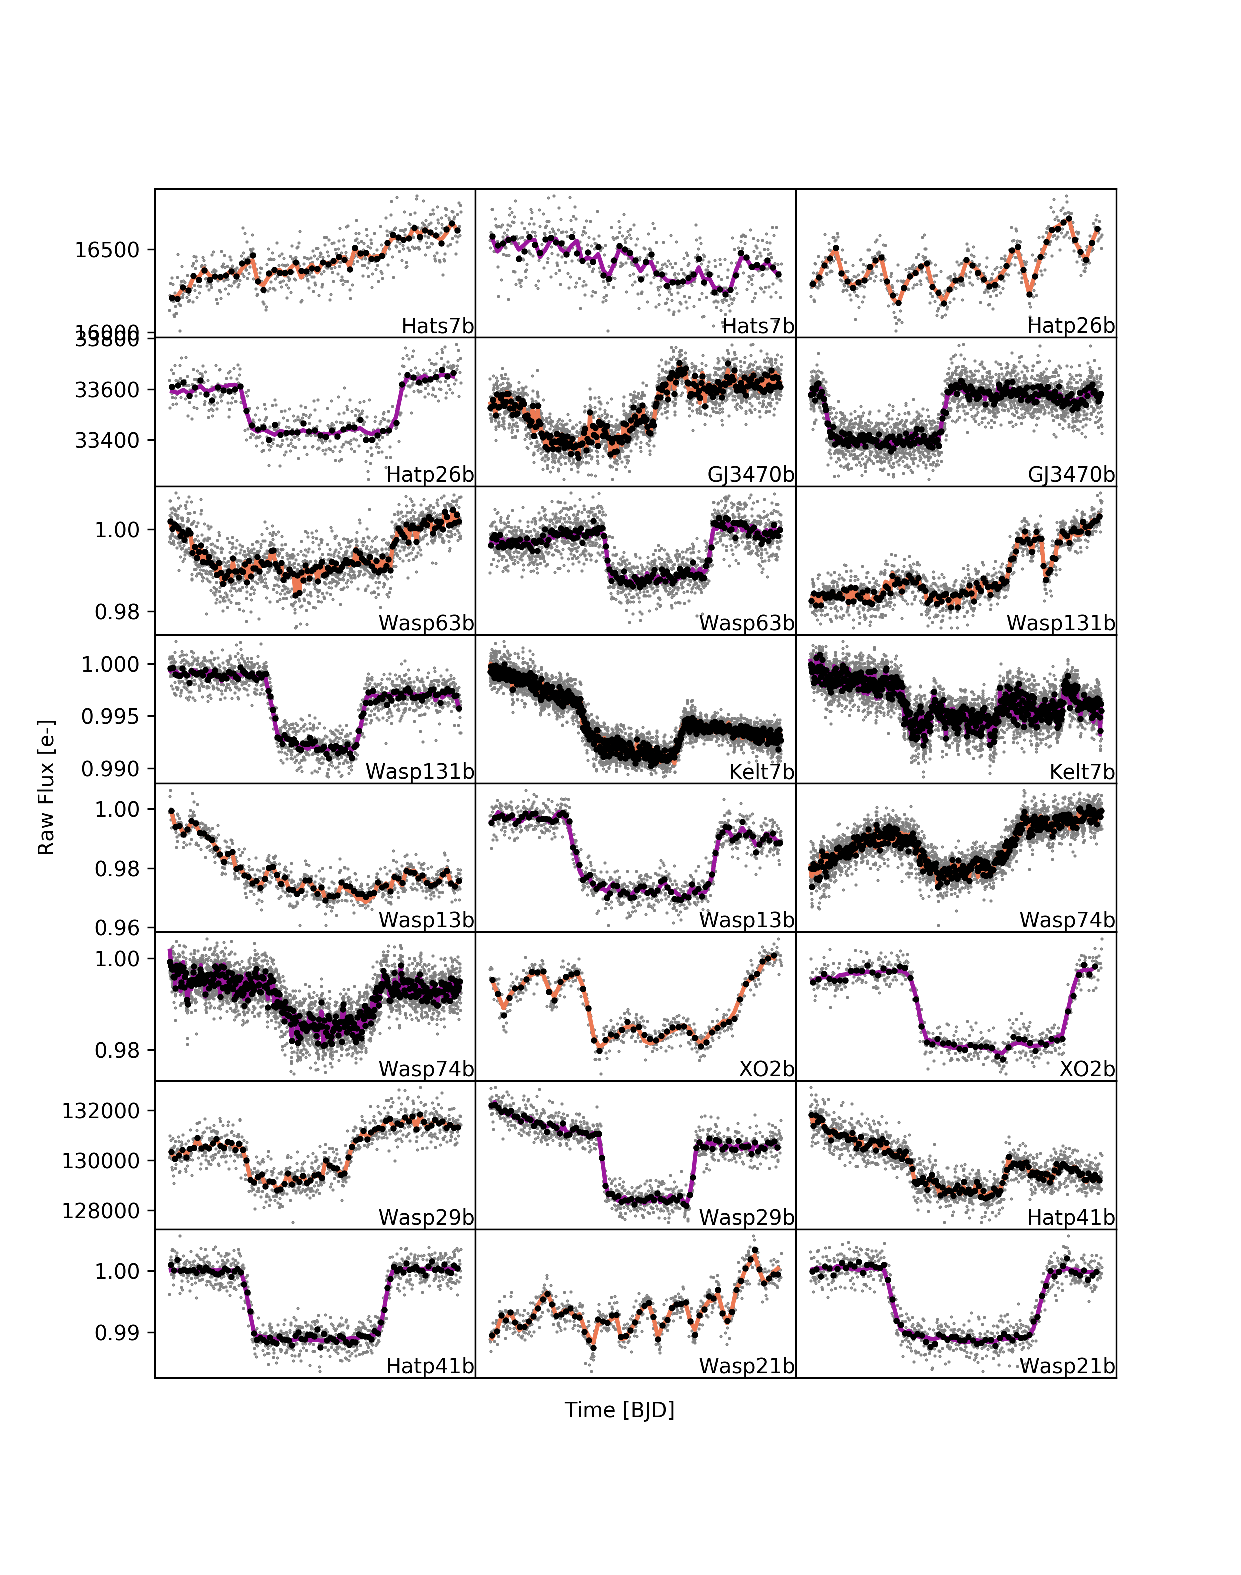
\includegraphics[width=\textwidth]{RawLighctuves0.pdf}
    \caption{Raw lightcurves for each planet. Flux binned in 5 minutes is show in black and 30 seconds is shown in gray. Colored lines indicate the best-fit instrumental and transit model from our MCMC analysis.}
  \end{figure*}

  \addtocounter{figure}{-1}
  \begin{figure*}
      %\label{P1:fig:rawlc1}
    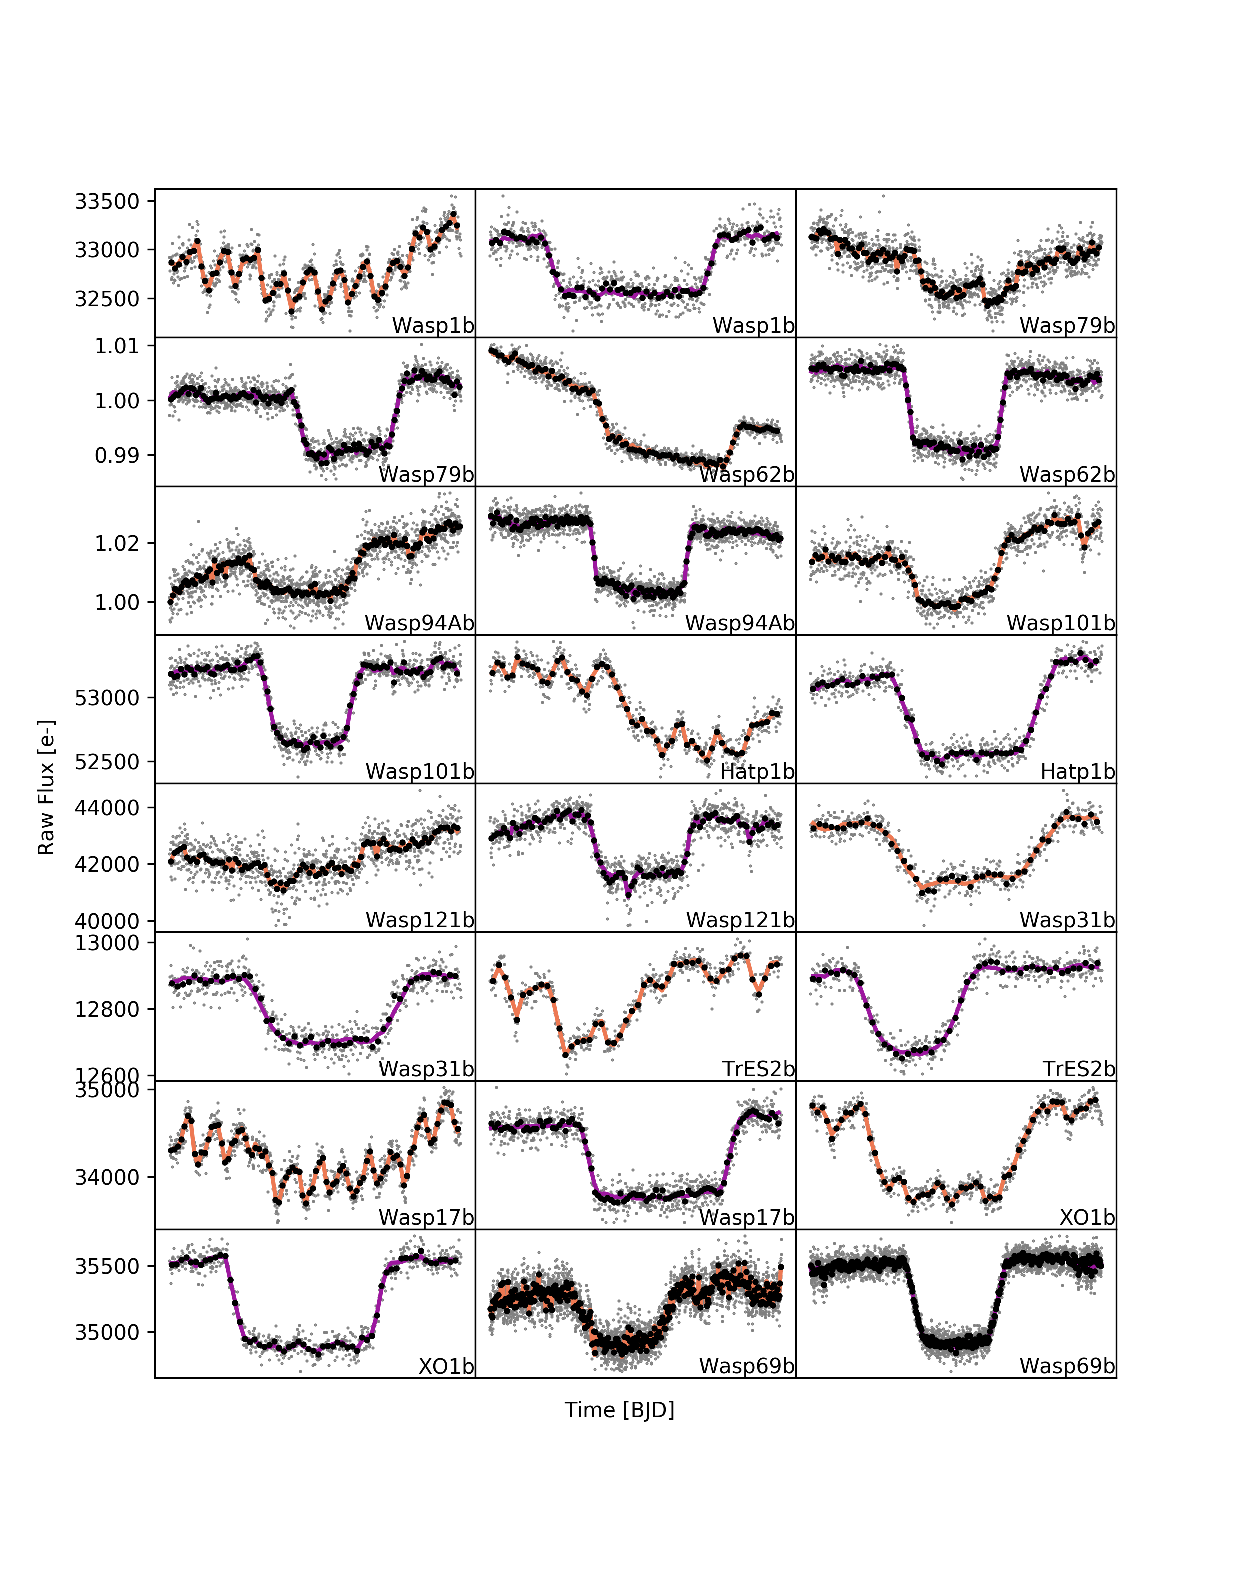
\includegraphics[width=\textwidth]{RawLighctuves1.pdf}
    \caption{\textit{Continued.}}
  \end{figure*}

  \addtocounter{figure}{-1}
  \begin{figure*}
      %\label{P1:fig:rawlc2}
    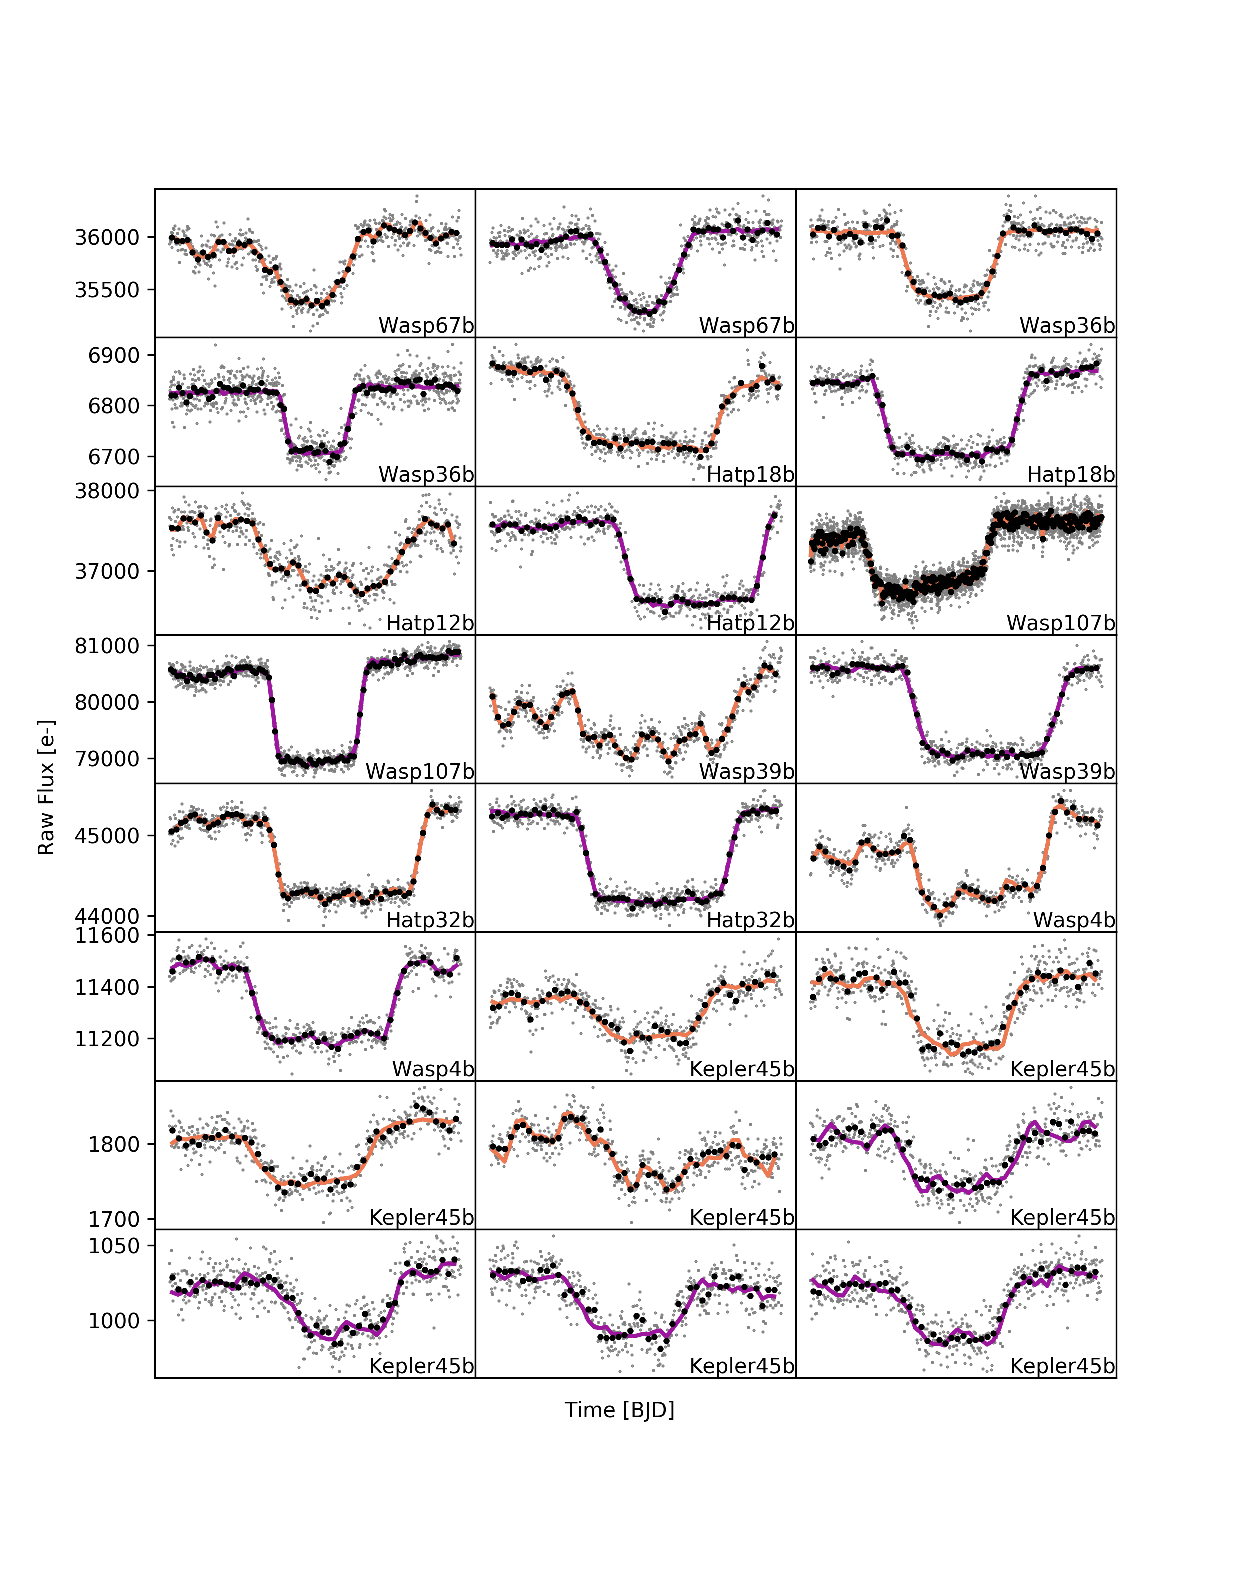
\includegraphics[width=\textwidth]{RawLighctuves2.pdf}
    \caption{\textit{Continued.}}
  \end{figure*}

  % \section{RMS vs Binsize}
  % \label{P1:app:rmsvsbinsize}

  \begin{figure*}
    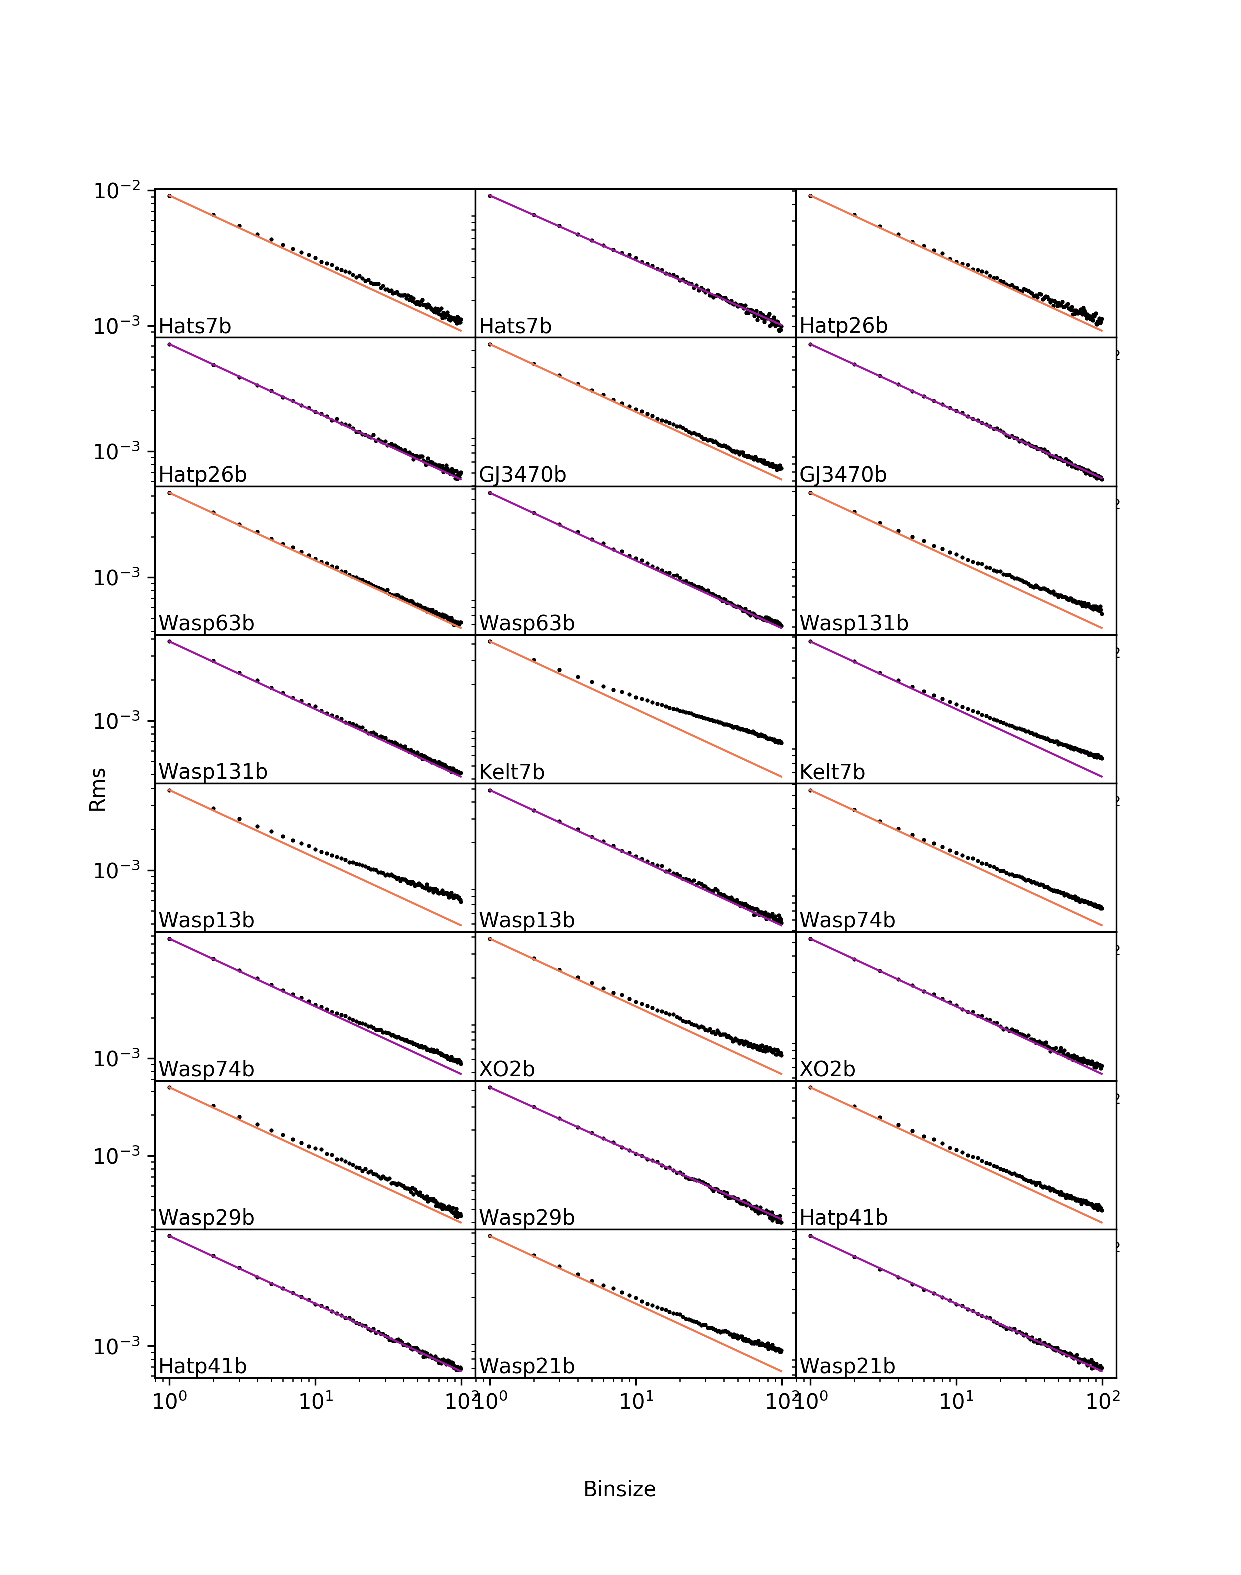
\includegraphics[width=\textwidth]{rmsVsbinsize0.pdf}
    \caption{RMS vs normalized binsize of each of the fitted lightcurves. Straight line is the sqrt(N) theoretical value.\label{P1:fig:rmsvsbin}}
  \end{figure*}

  \addtocounter{figure}{-1}
  \begin{figure*}
      %\label{P1:fig:rmsvsbin1}
    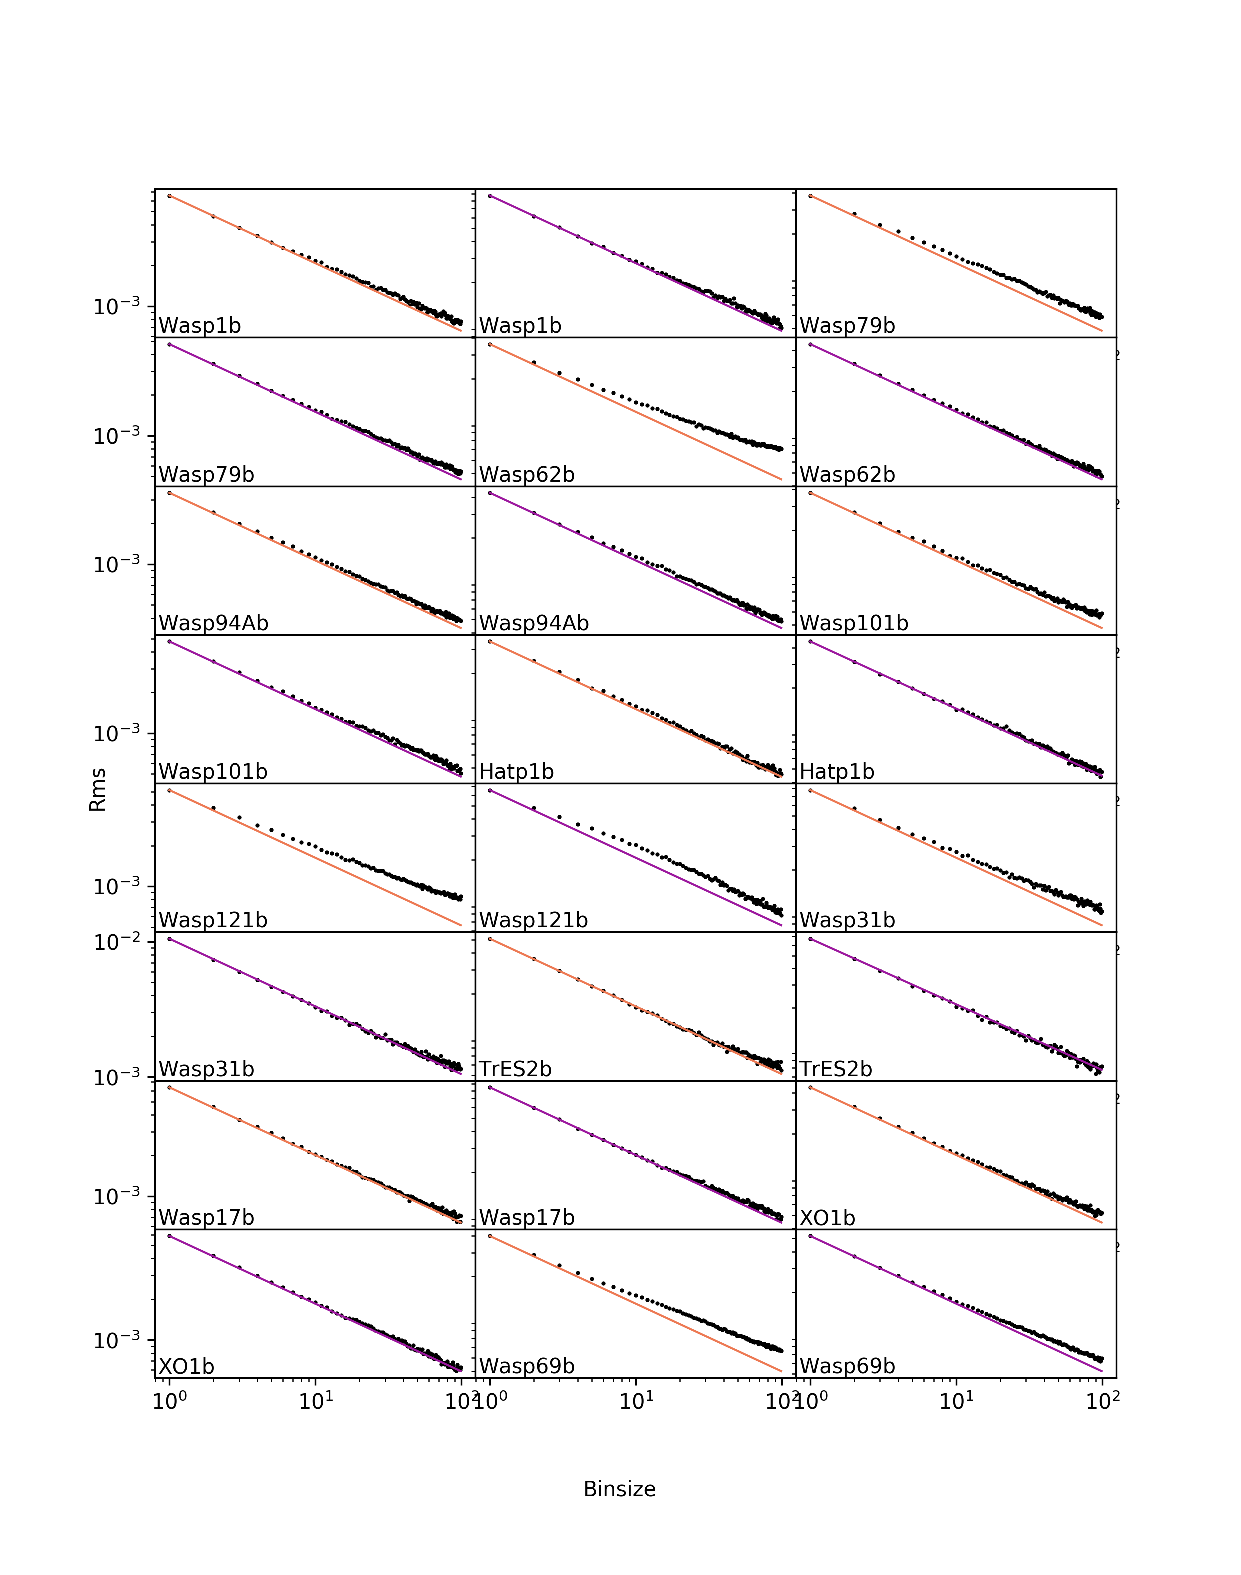
\includegraphics[width=\textwidth]{rmsVsbinsize1.pdf}
    \caption{\textit{Continued.}}
  \end{figure*}

  \addtocounter{figure}{-1}
  \begin{figure*}
      %\label{P1:fig:rmsvsbin2}
    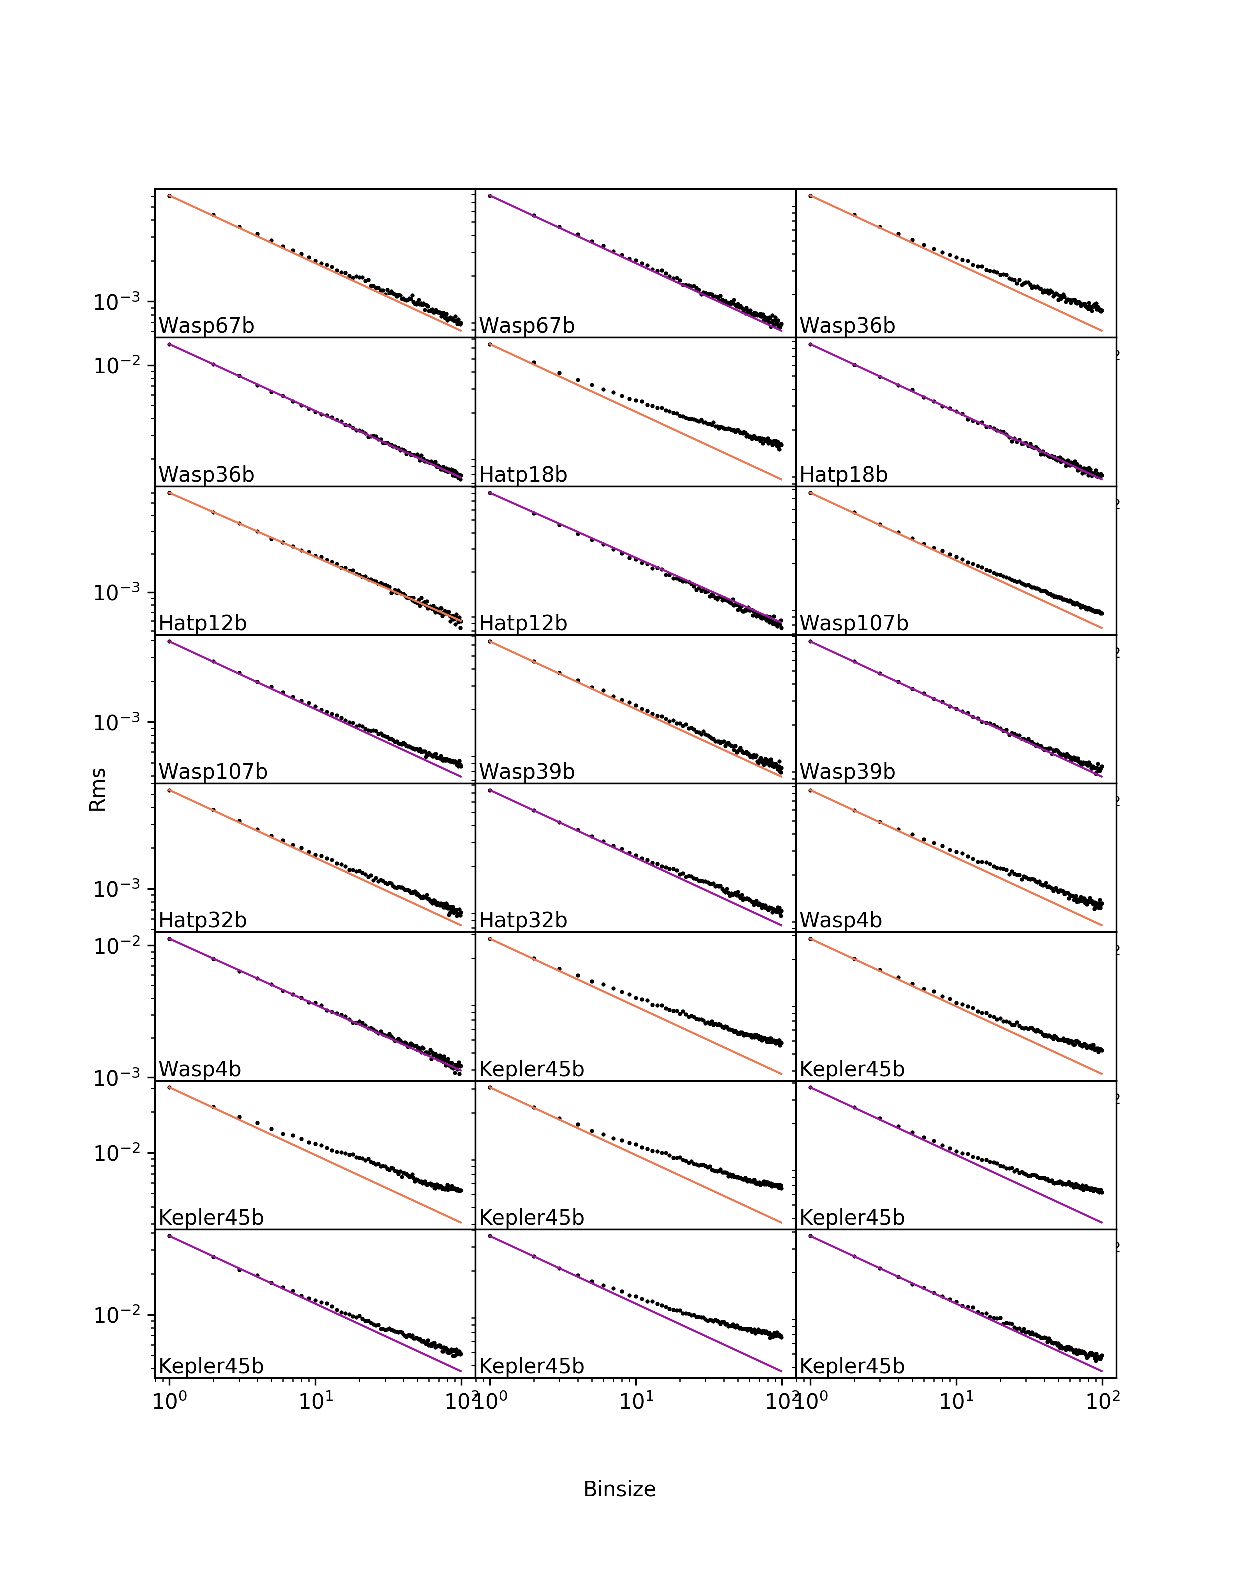
\includegraphics[width=\textwidth]{rmsVsbinsize2.pdf}
    \caption{\textit{Continued.}}
  \end{figure*}


  \section{VULCAN validation on HD 209458b}

  \begin{figure}
      \centering
      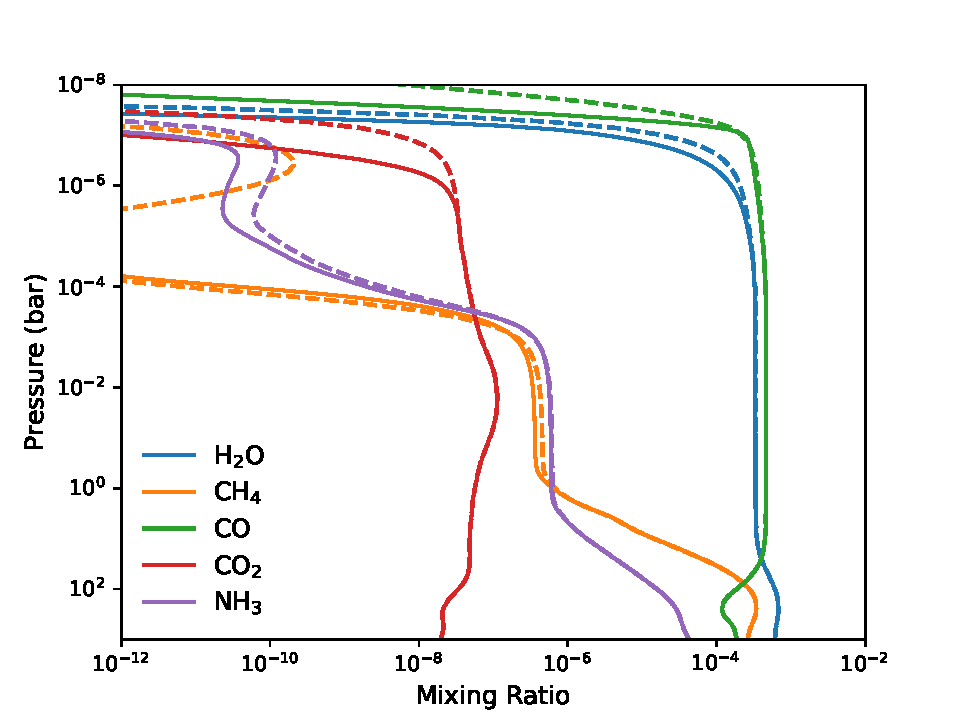
\includegraphics[width = \linewidth]{HD209-referee.pdf}
      \caption{Abundance mixing ratios at different pressures for the main species in the \spitzer bandpasses in HD 209458 b. The solid line shows the results from our VULCAN calculation and the dashed line the results from \citet{Moses2011}. The temperature and eddy-diffusion structure are taken the same as the dayside-average P-T profile in \citet{Moses2011}. The solar flux is also used as an analog for HD 290458 at a distance of 0.04747 AU.}
      \label{P1:fig:HD209}
  \end{figure}

  \section{Radius Anomaly}

  \begin{sidewaysfigure}
      \centering
      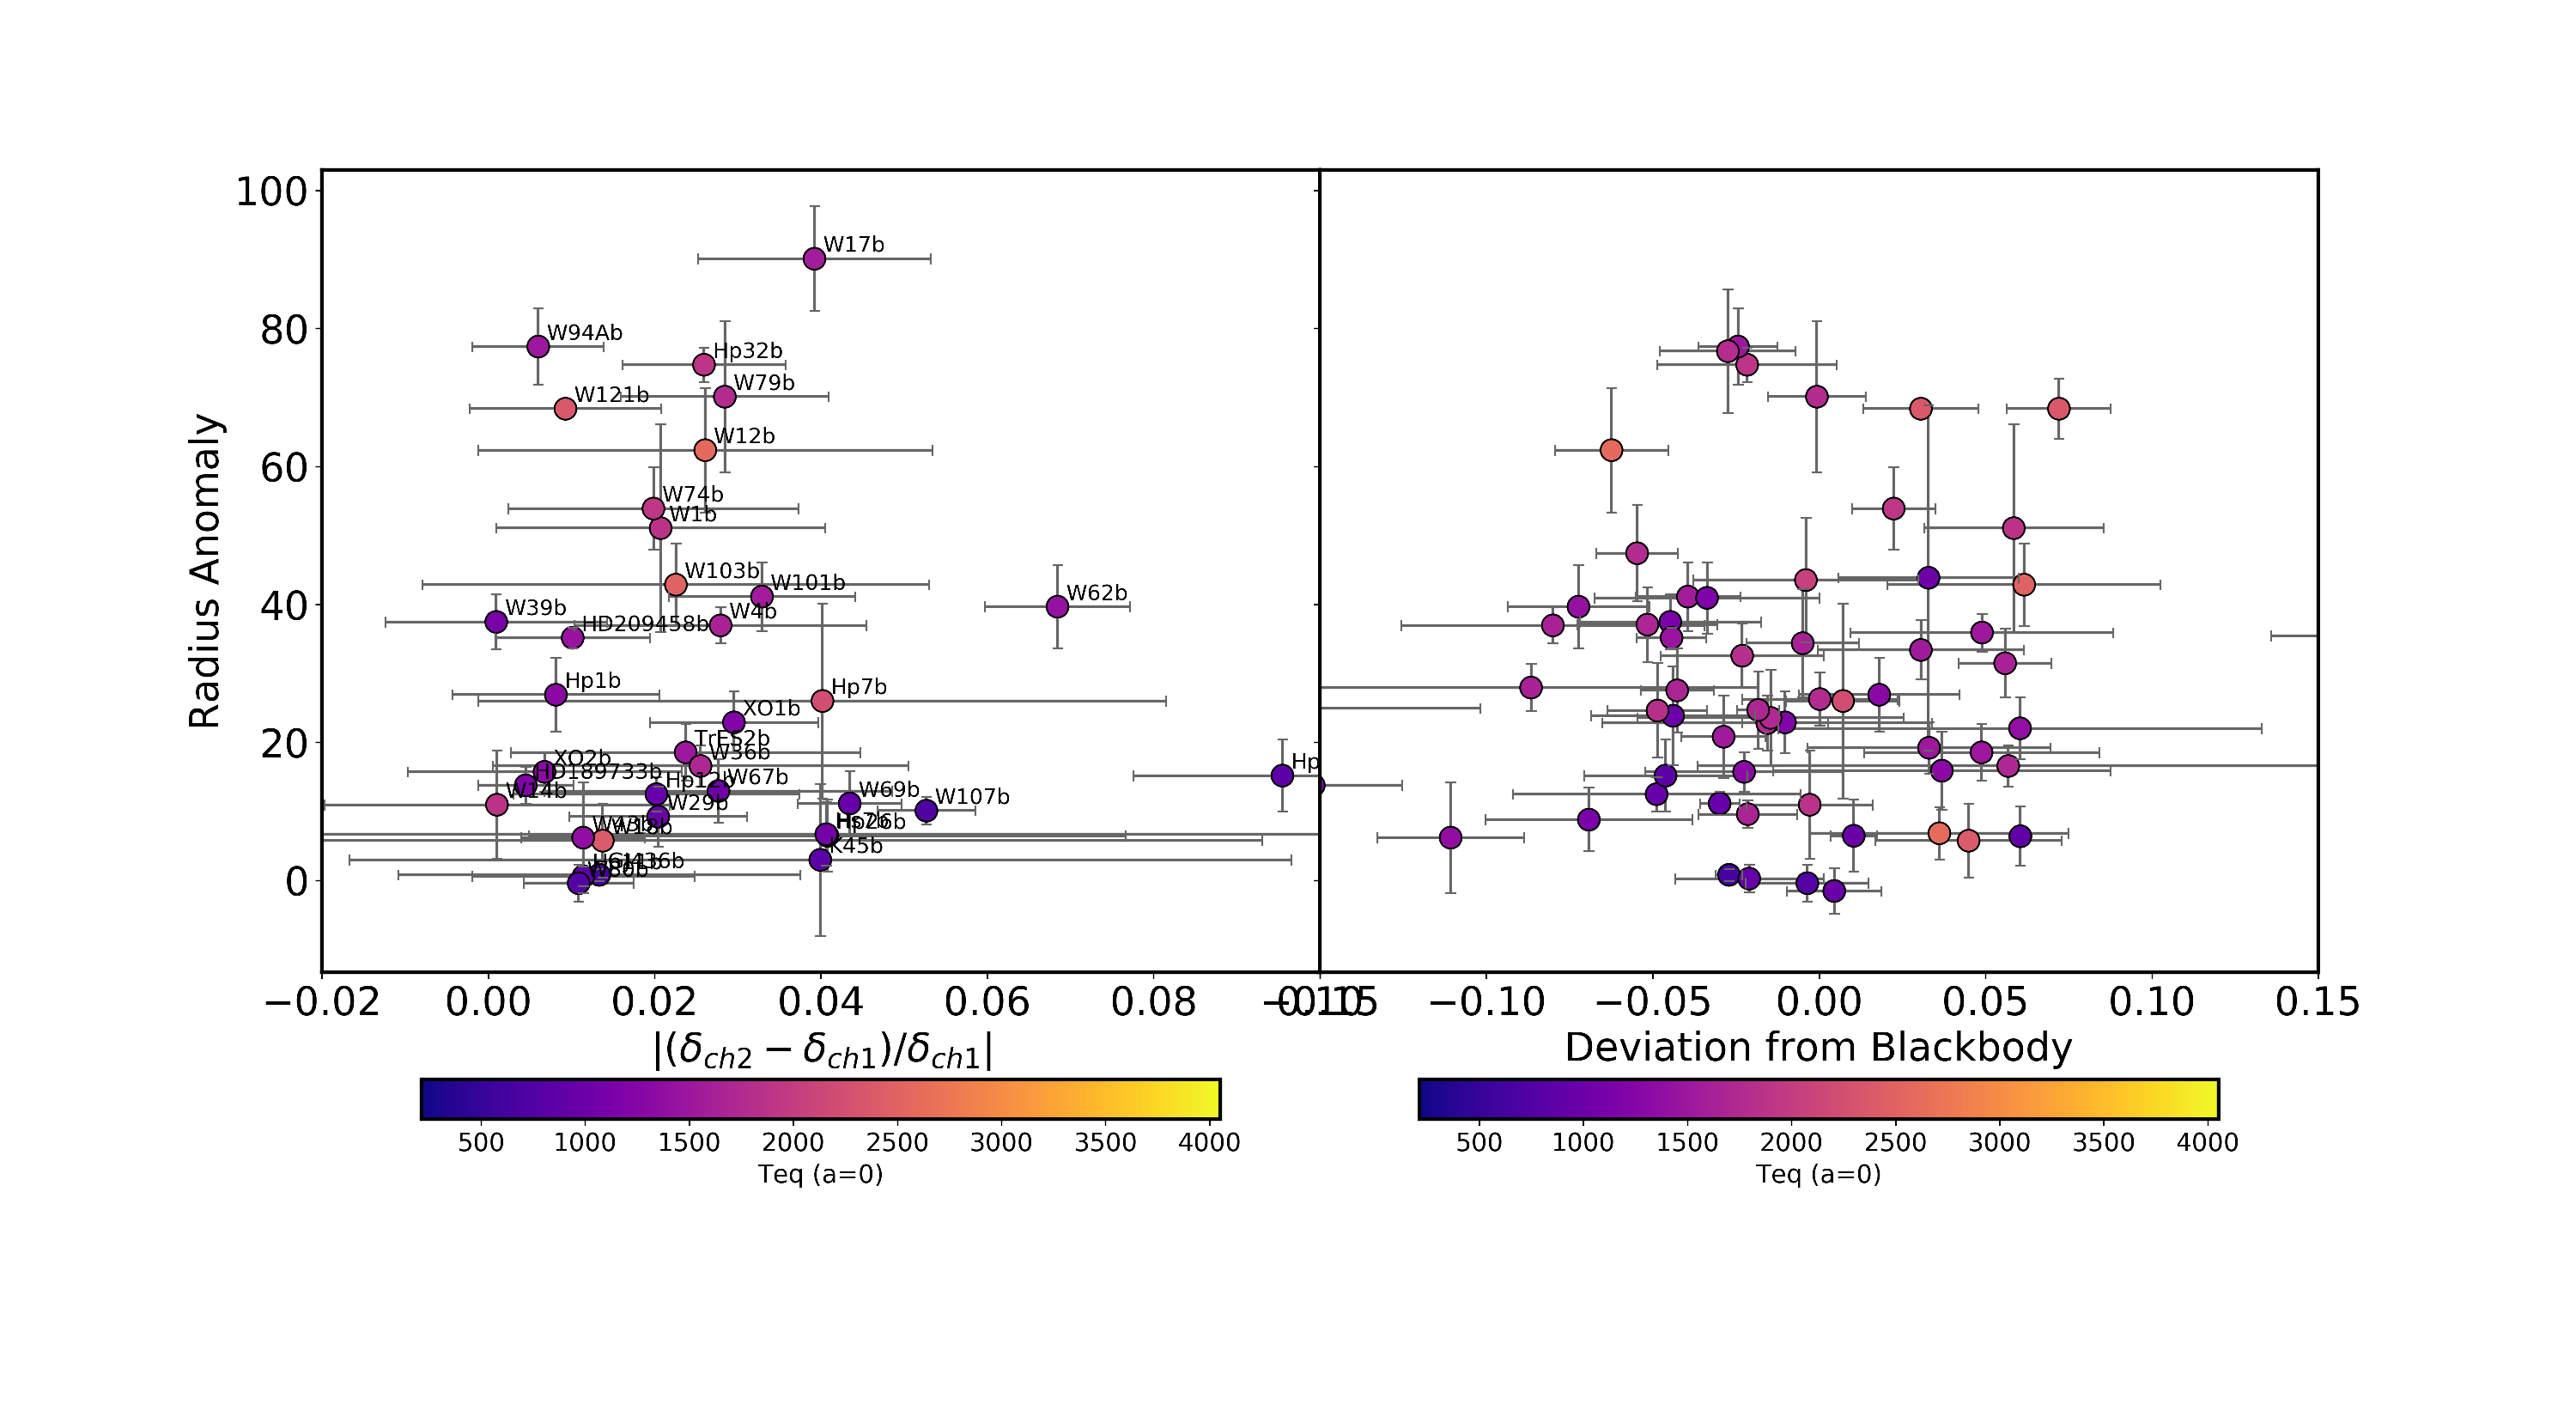
\includegraphics[width = \textwidth]{RadiusAnomaly.pdf}
      \caption{Radius Anomaly (calculated using models from \citet{Thorngren2016, Thorngren2018} against the absolute value of the normalized difference in transit depths for the available planets. Color scale is the equilibrium temperature of the planet.}
      \label{P1:fig:RadiusAnomaly}
  \end{sidewaysfigure}

\end{subappendices}



%%% Local Variables:
%%% mode: latex
%%% TeX-master: "../../main"
%%% End:

\include{content/chapter3/chapter3}
\chapter[Periodic variability in the brightness of an ultra-hot Jupiter atmosphere]{Periodic variability in the brightness of an ultra-hot Jupiter atmosphere}
\chaptermark{header title} %% if you want a different title in the headers
\label{w18b}

% Define the location of your plots
\graphicspath{{./gfx/Wasp18b/}}

% List all paper authors
\chauthors{Claire Baxter \&
          Jean-Michel D\'esert}

\chjournal{Astronomy \& Astrophysics, (to be submitted)}

\newcommand{\micron }{$\mu$m }
\newcommand{\CO}{\ce{CO}}
\newcommand{\water}{\ce{H2O}}
\newcommand{\methane}{\ce{CH4}}

\begin{abstract}
  % {} leave it empty if necessary
  \textit{Context} With close-in orbits and strong stellar irradiation on tidally locked daysides, hot Jupiter atmospheres are predicted to form large-scale weather structures. Observing the variability of a hot Jupiter is a key probe of such weather patterns as well as probing the atmospheric dynamics and temperature structures.\\
  % aims heading (mandatory)
  \textit{Aims} We aim to characterize the brightness variability of the ultra-hot Jupiter WASP-18b by analyzing ten secondary eclipses at 4.5~$\mu$m with Spitzer/IRAC.\\
  % methods heading (mandatory)
  \textit{Methods} Our observations span a time frame of 21.6 days which covers 23 planetary orbits. We search for temporal variability by robustly analyzing each of the lightcurves using our custom pipeline which implements pixel level decorrelation. We benchmark our results against the well-studied XO-3b.\\
  % results heading (mandatory)
  \textit{Results} We observe a variability in the eclipse depth with time, which is the first infrared temporal variability in secondary eclipse observations of hot Jupiters. Using a sinusoidal model, we derive a variability period of 23.12 $\pm$ 1.66 days and a peak-to-trough amplitude of 456 $\pm$ 71~ppm, corresponding to $\sim$12\% variability. We discuss possible causes of this variability, such as stellar variability, variable wind speeds, clouds, changes in atmospheric composition, and magnetic field coupling. We find that a 12\% variability signal would not be detected in the four available sectors of TESS containing WASP-18b, or with the 5 available HST/WFC3 eclipses, and that future observatories would be required for followup.
\end{abstract}

\section{Introduction}

Hot Jupiters are ideal targets for precise atmospheric characterization due to their large planet-to-star flux ratios. There have now been many secondary eclipse observations of hot Jupiters in the infrared, ranging from individual studies \citep[e.g.,][]{Charbonneau2005, Deming2005a} to large-scale survey programs \citep[e.g.,][]{Schwartz2017, Baxter2020, Garhart2020}. The vast majority of hot Jupiter atmospheres are expected to form clouds and photochemical hazes \citep{Sing2016, Parmentier2016, Wakeford2019}. Inhomogeneous coverage of such clouds could lead to brightness variability in time.

Temporal variations have been observed at 5~$\mu$m in the equatorial banded structures of Jupiter \citep{Antunano2019}. Variability in time is also common in cool brown dwarfs, with variability amplitudes of a few percent in more than 50\% of L and T brown dwarfs \citep{Metchev2015}. Furthermore, variability has also recently been detected on directly imaged free-floating planetary-mass objects \citep[e.g.,][]{Biller2015}. However, observing variability on directly imaged exoplanets is difficult due to the contrast between the host star and planet \citep{Apai2016}.

%Variability in hot Jupiters.
Nevertheless, atmospheric variability in time has been measured with phase curve observations of 3 hot Jupiters to date: HAT-P-7b \citep{Armstrong2016}, Kepler-76b \citep{Jackson2019}, and WASP-12b \citep{Bell2019}. \citet{Armstrong2016} use 4 years of public \textit{Kepler} data of HAT-P-7b to search for variability. They find temporal variations in the phase curve shape, including the hot-spot offset, such that the hot-spot shifts from one side of the substellar point to the other on timescales of tens to hundreds of days. However, they find only marginal evidence of brightness variability in time, which they note can be explained by systematic noise in their fits. Also using \textit{Kepler} data, \citet{Jackson2019} found similar phase offset variability in Kepler-76b, however, they do measure variability in the phase curve amplitude. Furthermore, two phase-curve observations at 3.6~$\mu$m taken 3 years apart of WASP-12b measure the phase curve offset to be $32.6 \pm 6.2^{\circ}$ eastward to $13.6 \pm 3.8^{\circ}$ westward \citep{Bell2019}.

% HD189 paper
To date, there has been no periodic brightness variability measured in secondary eclipse observations of hot Jupiters in the infrared. \citet{Agol2010} place an upper limit of 2.7\% at 8~$\mu$m on the eclipse depth variability of HD 189733b. Furthermore, \citet{Kilpatrick2020} carried out multi-epoch secondary eclipse observations with Spitzer/IRAC in an attempt to constrain the variability of HD 189733b and HD 209458b. They do not find a periodic variability signal, but they can place upper limit constraints on any possible variability to 12\% and 1.6\% at 4.5~$\mu$m for HD 189733b and HD 209458b respectively.

% Causes of variability
A possible cause of the variability on HAT-P-7b in the optical is variable wind speeds leading to variable cloud coverage \citep{Armstrong2016}. Similarly, \citet{Jackson2019} proposed the advance and retreat of thermal structures on Kepler-76b. This leads to cloud formation on the nightside blowing over to the dayside and creating a feedback loop resulting in periodic variability. \citet{Rogers2017} explored the effect of magnetic fields on HAT-P-7b by incorporating magnetohydrodynamics (MHD) into their global circulation models (GCMs). They conclude that coupling of the magnetic field with ionized species in the atmosphere can act against the eastward hot spot offset caused by the day-night temperature contrast. Such feedback can settle into an oscillating pattern on timescales of $\sim10^6$ seconds, creating the observed variability. In the case of WASP-12b, analysis of the 3.6 and 4.5~$\mu$m phase curves suggest mass-loss of the planet \citep{Bell2019}. Variability in the mass loss rate could be the cause of the phase offset variability. However, they also note that, following the arguments of \citet{Rogers2017}, variability due to magnetic coupling would be expected on WASP-12b.

In this paper, we measure and discuss the atmospheric brightness variability in the infrared of the ultra-hot Jupiter WASP-18b.

\section{Observations}

We observed ten secondary eclipses of WASP-18b at 4.5~$\mu$m with Spitzer/Infrared array camera (IRAC), program 11099 (PI: Kreidberg). Each observation consisted of 11776 exposures of 2-second integration in sub-array mode, resulting in 6.54 hours per lightcurves. Our observations were preceded with a scheduled 30-minute throw-away "peak-up" observation to obtain accurate pointing before the main observation to minimize the effect of IRACs well known intrapixel sensitivity. The ten eclipses span from 8th-30th September 2015, a total time of 21.65 days, corresponding to 23 orbits of WASP-18b, given its orbital period of 0.94124000 days \citep{Pearson2019}.

Furthermore, we also analyzed the ten eclipses of XO-3b, program 90032 (PI: Knutson), to test the robustness of our pipeline and our results, particularly on the variability. These eclipses were previously part of the repeatability and reliability data challenge presented in \citet{Ingalls2016}.

\section{Data Analysis}

\subsection{Spitzer/IRAC photometric lightcurve reduction}

We reduce the Spitzer/IRAC secondary eclipse lightcurves with our custom pipeline described fully in Baxter et al. (submitted.) which follows the analysis method from \citep{Deming2015}. For clarity, we recall the main steps of our pipeline. In each of the Spitzer subarray frames, we correct the dark current, flat field, and convert to flux units before performing aperture photometry using a circular aperture around the calculated centroid position of the star. %We also calculate the midtimes of each photometric point from the UTC-based modified barycentric Julian date (MBJD) times in the file headers.
A full run of our pipeline creates a grid of data reductions and finds the optimum methods and parameters for background subtraction, centroiding, and aperture photometry radius utilizing a lowest reduced $\chi^2$ on the resulting lightcurves. Uncertainties on the photometric points are calculated from photon noise and scaled up such that the reduced $\chi^2$ after an initial least-squares fit is equal to 1.
%Our pipeline also removes some data from the beginning of the observation, we run a sequence of cuts to determine how much data to remove to minimize the reduced $\chi^2$ and the root mean square (RMS) of the residuals of the resulting lightcurve.

Our resulting optimum pipeline reduction methods were to centroid using the barycenter method, with a box size of 3x3, calculate the background using 4 pixels in each of the 4 corners of the image, and to perform aperture photometry with a radius of 2.5 pixels around the star. In each lightcurve, we masked between 0.053\% and 0.076\% bad pixels at 4$\sigma$. We also removed 15 minutes from the beginning of each of the lightcurves to remove the peak-up period of the observations. The best raw normalized photometric lightcurve for each observation is then used in the next step for a complete statistical analysis of the transit/eclipse parameters.

\subsection{Spitzer/IRAC secondary eclipse fitting}
\label{P3:sec:fitting}

To find the eclipse parameters from the raw photometric lightcurve, we fit a batman eclipse model \citep{Kreidberg2015} in combination with a temporal quadratic function (\nth{1} or \nth{2} order) and a pixel level decorrelation (PLD) systematic model \citep{Deming2015}. In our fit of WASP-18 b, we fix the period to 0.9414529 $\pm$ 0.00000234 \citep{Pearson2019} and the eccentricity and angle of periastron passage to 0.
% We also fix the parameters of a linear limb darkening law with limb darkening parameters calculated from the 1D ATLAS code presented in \citep{Sing2010} to 0.1601736 $\pm$ 0.00466754 at 4.5~$\mu$m. The stellar parameters use for this calculation were: 6400$\pm$100, 4.366$\pm$0.026, 0$\pm$0.1 for the effective temperature, surface gravity and metallicity respectively, taken from \citep{Southworth2009}.

Typically, the PLD systematic model uses a 3x3 grid of pixels around the centroid of the star to model the systematics. Since WASP-18b is a bright star, a significant portion of the stellar PSF may spread beyond these nine pixels, we, therefore, test the effect of including more pixels with a 5x5 PLD grid. However, we found that a 5x5 PLD box compared to a 3x3 PLD box was not improving the fits.
%necessary as it resulted in overfitting (mean $\Delta$BIC over 10 lightcurves is -960).

Furthermore, since assuming a \nth{1} order quadratic (linear) baseline can result in underestimating the eclipse depth for hot planets with large phase amplitudes \citep[e.g.,][]{Bell2019}, we also tested a \nth{2} order quadratic baseline in time. However, such a \nth{2} order quadratic coefficient can also be degenerate with the eclipse depth. We tested including a \nth{2} order quadratic baseline (2 free parameters) compared to a \nth{1} order baseline (1 free parameter). We found that it was not statistically significant to have a \nth{2} order quadratic free in each of the fits (mean $\Delta$BIC of 3). However, we also tested fixing the \nth{2} order quadratic co-efficient while still leaving the \nth{1} order co-efficient free. This test was statistically significant (mean $\Delta$BIC of 53) when comparing it with a \nth{1} order quadratic (linear) baseline. We, therefore, opted to fix the \nth{2} order coefficient to the weighted mean value from the first fit, -0.031 $\pm$ 0.004. This method corrects the astrophysical signal from the large phase amplitudes (\nth{2} order) without compromising the systematic correction (\nth{1} order) and thus leads to accurate results on the eclipse depths.

To achieve our final results we perform two fits of the lightcurves. First, we perform an initial fit with 15 free parameters ($a/R_s$, inclination, $F_p/F_s$, $T_{secondary}$, 9 PLD parameters and a \nth{2} order quadratic baseline in time). Then we fix $a/R_s$, inclination and the \nth{2} order quadratic coefficient to the weighted mean over all ten lightcurves. We do this since we do not expect these parameters to be physically changing in time. Our final MCMC fits have 12 free parameters ($R_p/R_s$, $T_{secondary}$, 9 PLD parameters and 1 temporal slope). As a sanity check, we compare the brightness temperatures between the first and second fit in Figure \ref{P3:app:depths}, and find that it still shows variability.

Posterior distributions and uncertainties are calculated on the fitted parameters by performing a full Markov Chain Monte Carlo (MCMC) exploration of parameter space using emcee \citep{Foreman-Mackey2013}. We run chains with 100 walkers with a typical 500 step burn-in period followed by a 1000 step production run and confirm the convergence of our chains via the auto-correlation time and the mean acceptance fraction.

\section{Results}
\subsection{Spitzer/IRAC secondary eclipse lightcurves}
\label{P3:sec:lcresults}

Table \ref{P3:tab:resutls} displays the $a/R_s$, inclination and \nth{2} order quadratic coefficient from the first fit alongside
% We do not find any variability in $a/R_s$ and inclination with time, so we fix these parameters to the weighted mean for the second fit. Additionally, we find that the \nth{2} order quadratic coefficient is degenerate with the eclipse depth and results in a worse BIC, so we also fix this to the weighted mean as mentioned in Section \ref{P3:sec:fitting}.
$F_p/F_s$, $T_{secondary}$ and $T_B$ from the second fit. Figure \ref{P3:fig:correctedlcs} shows the final resulting systematic corrected lightcurves. We find that the weighted mean eclipse depth is 3729 $\pm$ 56~ppm, which is consistent with the eclipse presented in \citet{Nymeyer2011} and the phase curve presented in \citet{Maxted2013}. We also find that the weighted mean secondary eclipse timings are within 1$\sigma$ agreement with the previously calculated eclipse ephemeris from \citet{Maxted2013}. Raw lightcurves and residuals are shown in Appendix \ref{P3:app:plots}.

\begin{figure}
    \centering
    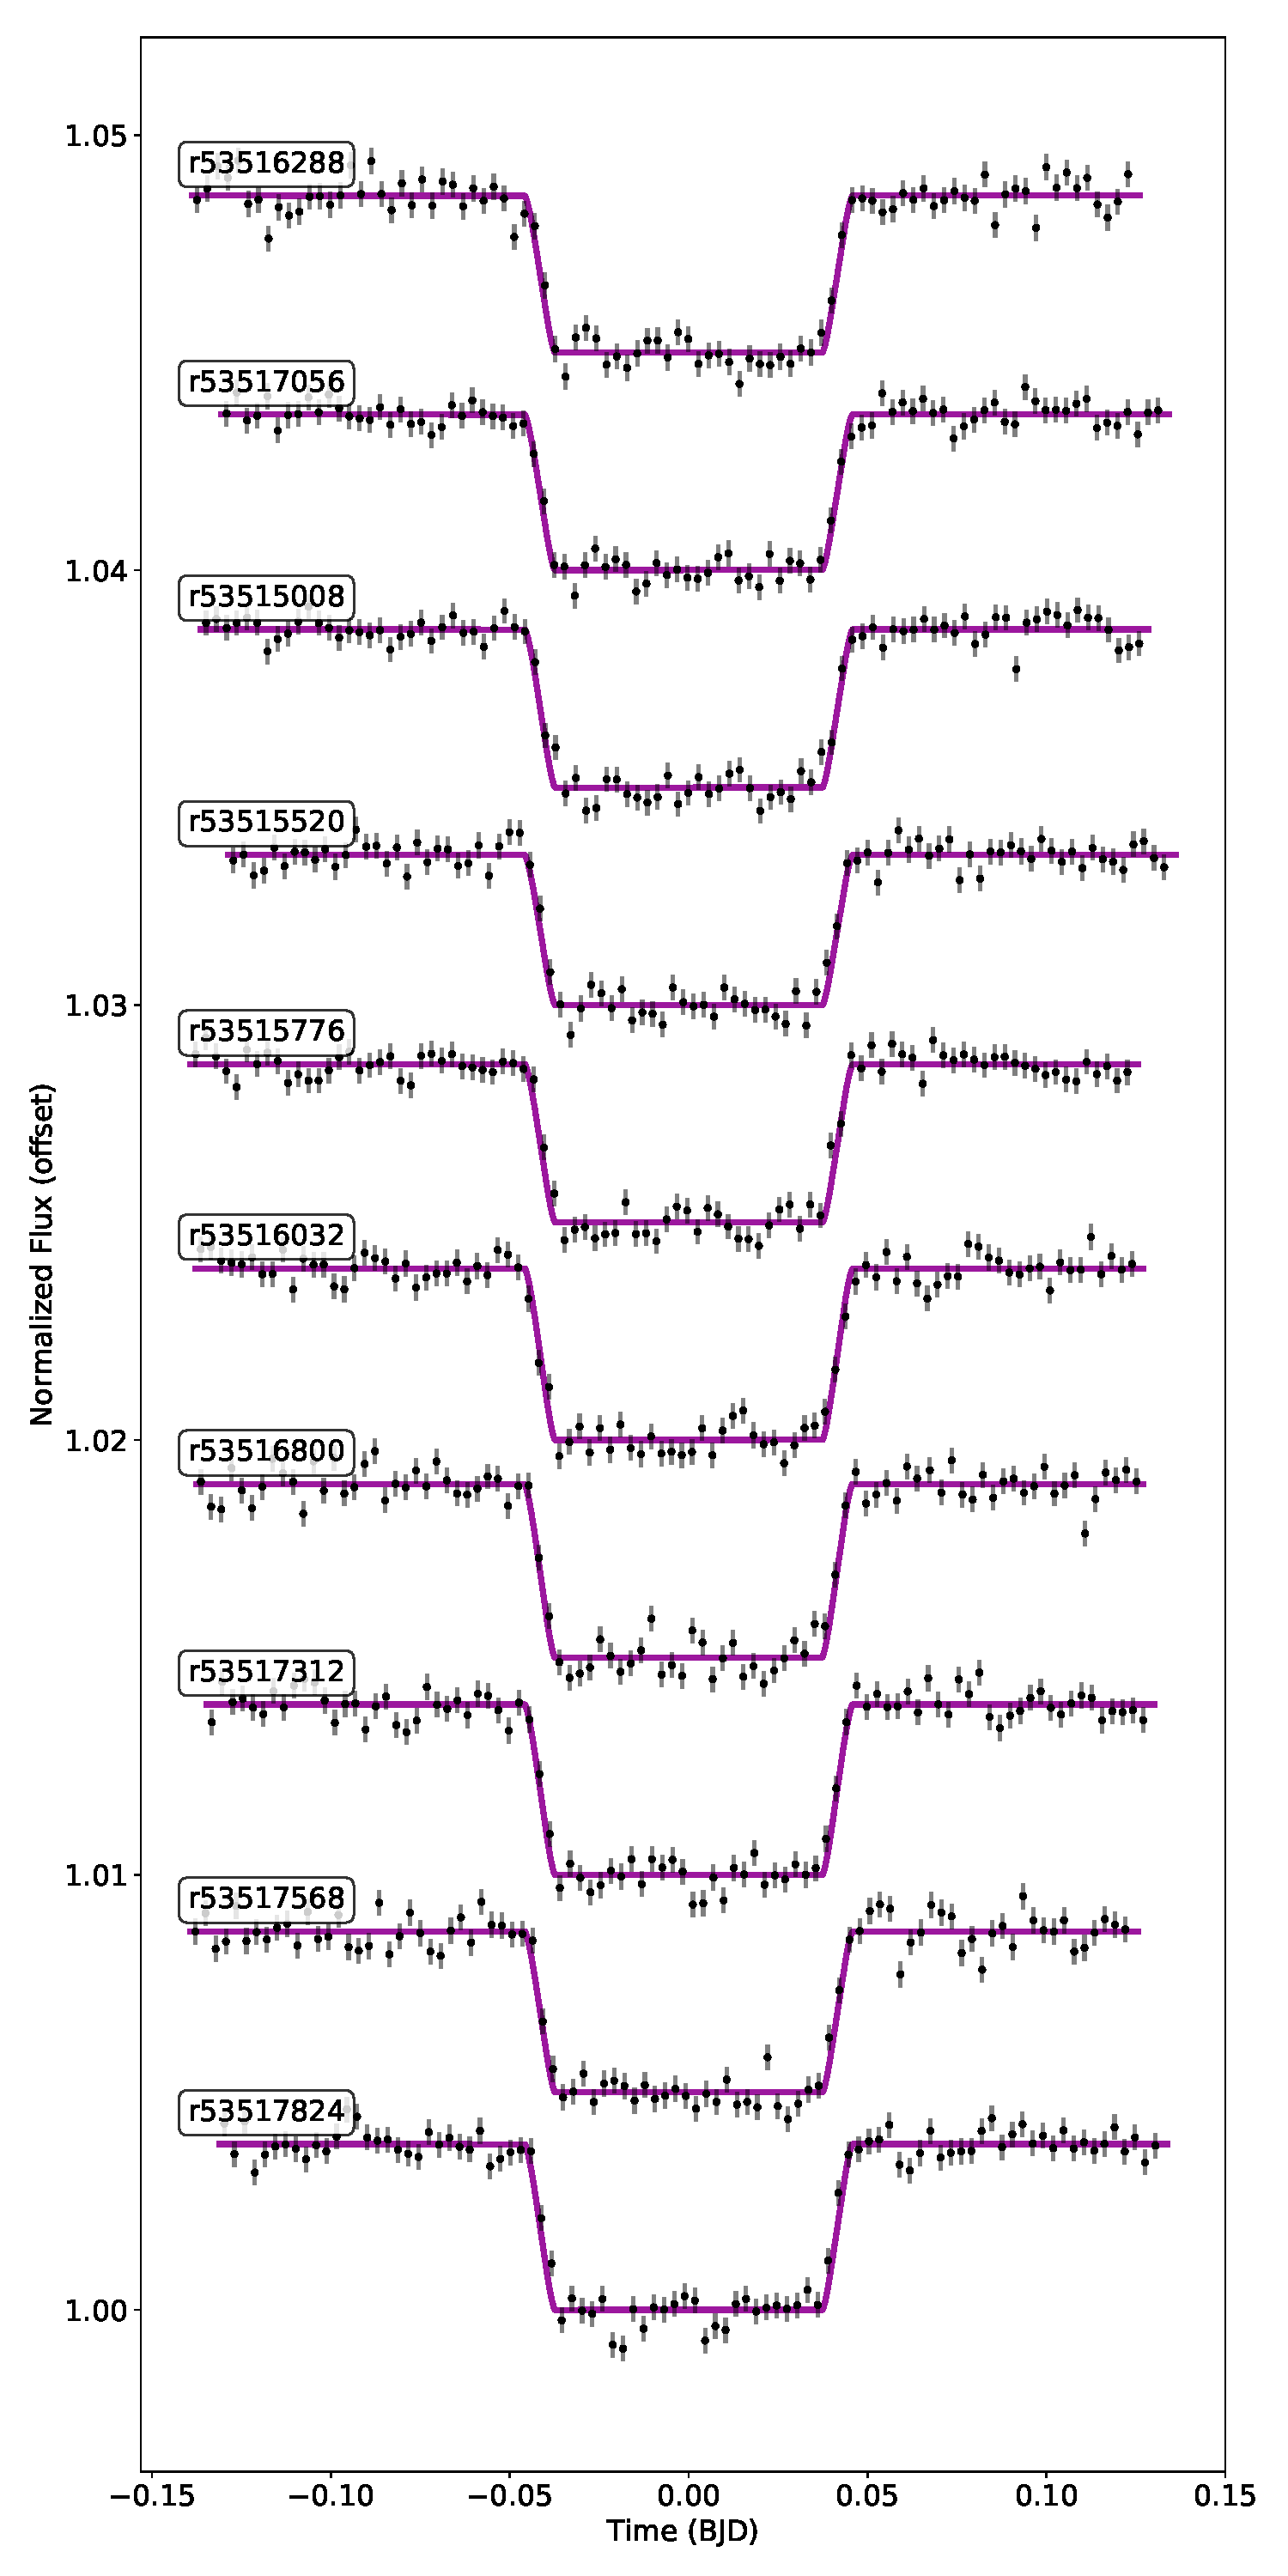
\includegraphics[height=\textheight]{Correctedlightcurves_W18b.pdf}
    \caption{Normalized and corrected eclipse lightcurves of WASP-18b, vertically offset for display purposes. These lightcurves are from the final fit, where we fixed $a/R_s$, inclination and the \nth{2} quadratic coefficient to their weighted means from the first fit. }
    \label{P3:fig:correctedlcs}
\end{figure}

\begin{landscape}
\begin{table*}[]
    \centering
    \caption{Best fit eclipse and systematic parameters using an MCMC method. The semi-major axis ($a/R_s$), inclination and 2nd order quadratic co-efficient (h) are shown from the first fits, they are fixed to the weighted mean in the final fit. The eclipse depth ($F_p/F_s$), brightness temperature ($T_B$) and the time of secondary eclipse ($T_{secondary}$) are shown from the final fits.}
    \label{P3:tab:resutls}
\begin{tabular}{lccc|ccc}
\hline \hline
 AOR & $a/R_s$ & Inclination & h & $F_p/F_s$ & $T_B$ & $T_{secondary}$ \\
 &  & Degrees & &~ppm & Kelvin & BJD \\
\hline
r53517824 & 3.48 $\pm$ 0.15 &  83.29 $\pm$ 2.05 &   -0.03 $\pm$ 0.008 &  3810 $\pm$ 68 &  3079 $\pm$ 37 &  2457274.14104 $\pm$ 0.00029 \\
r53517568 & 3.46 $\pm$ 0.14 &  83.38 $\pm$ 1.95 &  -0.039 $\pm$ 0.008 &  3700 $\pm$ 68 &  3011 $\pm$ 37 &   2457275.08202 $\pm$ 0.0003 \\
r53517312 & 3.43 $\pm$ 0.16 &  83.09 $\pm$ 2.22 &   -0.035 $\pm$ 0.01 &  3919 $\pm$ 78 &  3166 $\pm$ 41 &  2457278.84855 $\pm$ 0.00028 \\
r53516800 & 3.34 $\pm$ 0.15 &  82.04 $\pm$ 1.94 &  -0.038 $\pm$ 0.008 &  3984 $\pm$ 66 &  3163 $\pm$ 36 &  2457279.78877 $\pm$ 0.00026 \\
r53516032 & 3.15 $\pm$ 0.15 &  80.42 $\pm$ 1.75 &  -0.011 $\pm$ 0.009 &  3954 $\pm$ 69 &  3147 $\pm$ 37 &  2457283.55482 $\pm$ 0.00028 \\
r53515776 & 3.48 $\pm$ 0.14 &  83.27 $\pm$ 1.85 &  -0.041 $\pm$ 0.008 &  3640 $\pm$ 68 &  2984 $\pm$ 38 &  2457286.37946 $\pm$ 0.00028 \\
r53515520 & 3.28 $\pm$ 0.18 &  81.15 $\pm$ 2.26 &  -0.046 $\pm$ 0.009 &  3454 $\pm$ 70 &  2890 $\pm$ 37 &  2457288.26257 $\pm$ 0.00029 \\
r53515008 & 3.06 $\pm$ 0.18 &   78.70 $\pm$ 2.09 &  -0.028 $\pm$ 0.009 &  3633 $\pm$ 67 &  2988 $\pm$ 35 &   2457289.2035 $\pm$ 0.00029 \\
r53517056 & 3.32 $\pm$ 0.19 &  82.08 $\pm$ 2.41 &  -0.025 $\pm$ 0.008 &  3585 $\pm$ 71 &  2943 $\pm$ 37 &  2457293.91153 $\pm$ 0.00031 \\
r53516288 & 3.38 $\pm$ 0.18 &  82.32 $\pm$ 2.27 &  -0.013 $\pm$ 0.009 &  3616 $\pm$ 69 &  2973 $\pm$ 38 &   2457295.79433 $\pm$ 0.0003 \\
\hline
Weighted Mean & 3.45 $\pm$ 0.04 & 81.96 $\pm$ 0.49 & -0.031 $\pm$ 0.004 & 3729 $\pm$ 56 & 3033 $\pm$ 31 & \\
\hline
Standard Deviation & 0.13 & 1.43 & 0.01 & 169 & 93 & \\
Mean Error & 0.16 & 2.08 & 0.01 & 69 & 37 & \\
\hline
\end{tabular}

\end{table*}
\end{landscape}

\subsection{Brightness variability of WASP-18b in time}

% Compare to a straight line.
We plot the secondary eclipse depths of WASP-18b in time (see Figure \ref{P3:fig:variability}), and we find that the eclipse depths are not constant, but instead they show a level of variability, that isn't random, but that is reproduced by a periodic sinusoidal signal. We find that the eclipse depth measurements deviate from a straight line by more than 7$\sigma$. We fit this temporal brightness variability with a sinusoidal function in time (t).
%We parameterize the sinusoid with three free parameters: amplitude (A), frequency ($\nu$) and an offset ($\bar{D}$). We tested having an additional phase parameter ($\varphi$) but this did not significantly improve the fits ($\Delta$BIC = 2.2). Therefore, we fixed phase to zero such that the eclipse depths in time are modeled by the following equation: D = Asin($\nu$t) + $\bar{D}$.
We parameterize the sinusoid with four free parameters: semi-amplitude ($A$), frequency ($\nu$), phase ($\varphi$) and an offset ($\bar{D}$) such that the eclipse depths in time are modeled with $D(t)$ = $A$sin($\nu$t) + $\bar{D}$. We tested fixing the phase parameter ($\varphi$) but this did not significantly improve the fits ($\Delta$BIC = 2.2).
We calculate posterior distributions on these parameters by running an MCMC exploration using emcee \citep{Foreman-Mackey2013} with 300 walkers, 1000 burn-in steps and 20000 production steps. We confirm convergence of the chains using the auto-correlation time and the mean acceptance fraction. We then test the robustness of our sinusoidal fit by comparing it with a straight line using the Bayesian Information Criteria (BIC).

Figure \ref{P3:fig:MCMCcorner} shows the posterior distributions from the MCMC sinusoidal fits and the best sinusoidal fit is also shown in Figure \ref{P3:fig:variability}. We find that the sinusoidal fit is statistically significantly favored over a straight line fit where BIC of the straight line being 62.3 and the BIC of the sinusoid being 18.2.
% The best fit sinusoidal parameters are: A = -0.00023 $\pm$ 3.5e-05, $\nu$ = 0.27 $\pm$ 0.019, $\varphi$ = 3.1 $\pm$ 0.23, $\bar{D}$ = 0.0037 $\pm$ 2.3e-05. This corresponds to a 23.16 $\pm$ 1.73 days period of variability and a 228.39 $\pm$ 35.23~ppm amplitude of variability. The weighted mean eclipse depth of all 10 eclipses results in an eclipse depth of 3725 $\pm$ 57~ppm, meaning the measured variability amplitude is 6.1$\pm$0.9\%.
The best fit sinusoidal parameters are: $A$ = 228$\pm$36~ppm, $\nu$ = 0.27$\pm$0.02, $\varphi$ = -0.01$\pm$0.23, $\bar{D}$ = 3732$\pm$23~ppm. This corresponds to a 23.1$\pm$1.7 days period of variability and a 12.2$\pm$1.9\% peak-to-trough brightness variability (2$A$).

We tested for variability and correlations with the other parameters we let free in the fits. The standard deviation is smaller than the mean error over all ten lightcurves for $a/R_s$ and inclination (see Table \ref{P3:tab:resutls}. This indicates that there is no variability in these parameters. We also tested for correlations between $a/R_s$ and inclination with $F_p/F_s$, in both cases they had low Pearson correlation coefficients (0.05 and 0.13 respectively) with high associated chance probabilities (0.9 and 0.7 respectively). These numbers indicate that $a/R_s$ and inclination are not correlated with $F_p/F_s$.

\begin{sidewaysfigure}
    \centering
    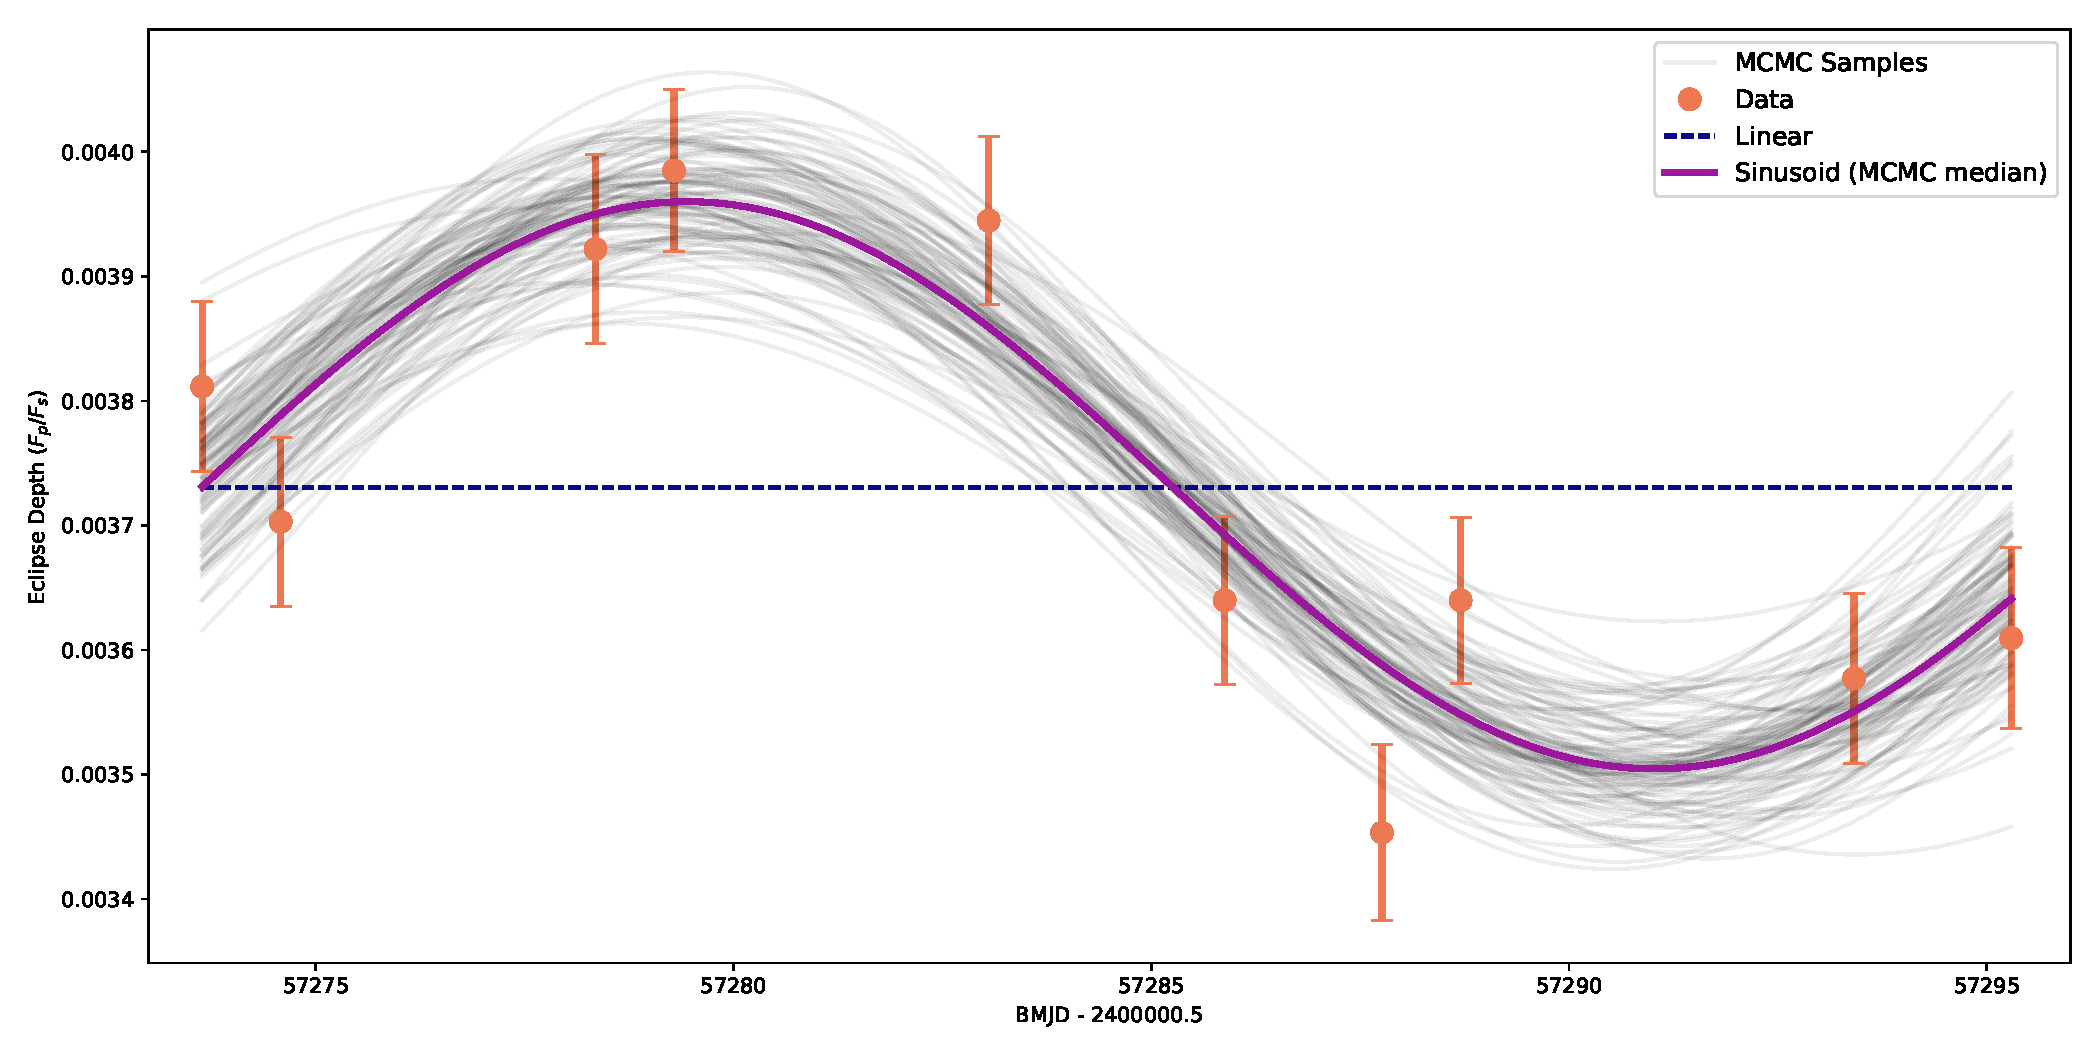
\includegraphics[width=\linewidth]{MCMCvarsamples.pdf}
    \caption{Measured eclipse depths of WASP-18b over time in orange, for the ten semi-consecutive eclipses. Purple solid line shows the median result from the MCMC fit, 100 random samples from the posterior distributions are shown in gray, blue line shows the best fitting straight line.}
    \label{P3:fig:variability}
\end{sidewaysfigure}

\begin{figure}
    \centering
    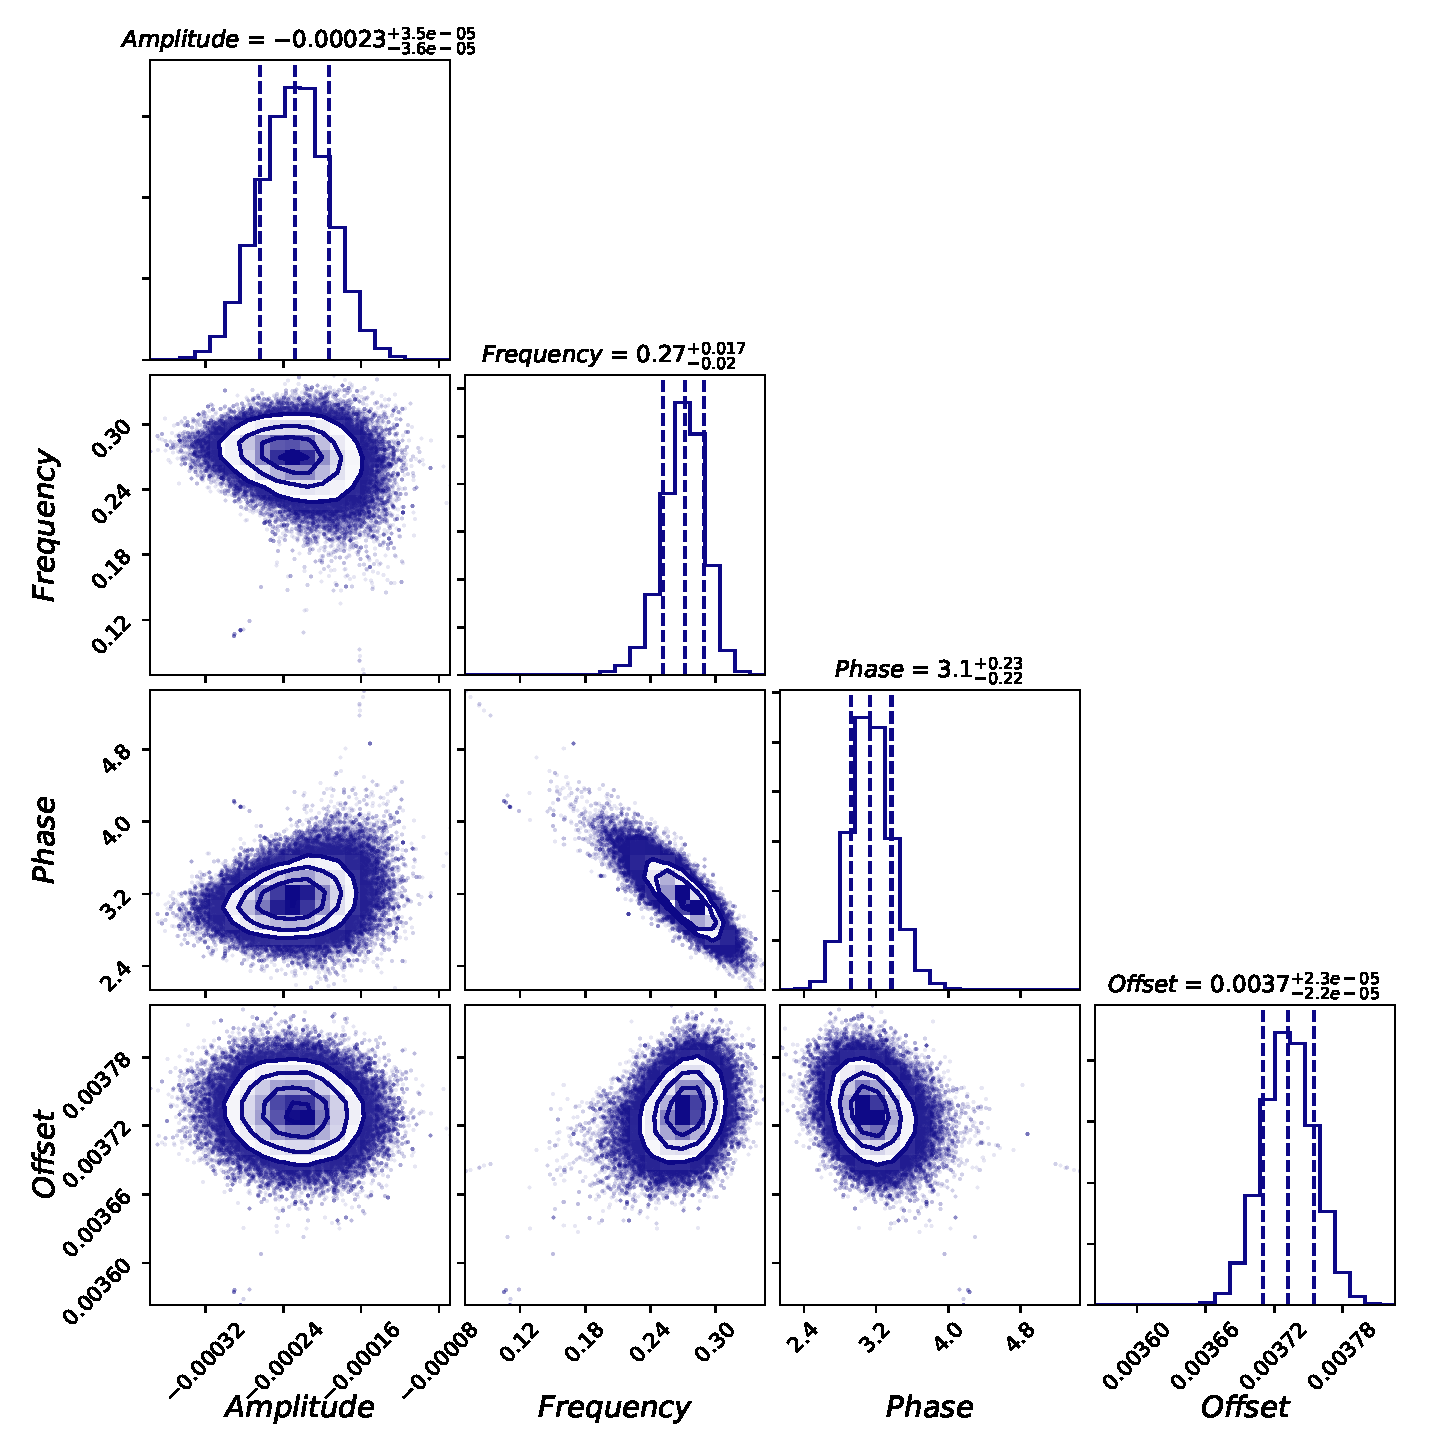
\includegraphics[width=\linewidth]{MCMCcorner.pdf}
    \caption{Posterior probability distributions of the free parameters from a periodic sinusoidal MCMC fit to the brightness variability in time of WASP-18b at 4.5~$\mu$m. In the marginalized confidence intervals the inner dashed line is the median and the outer dashed lines are the 1$\sigma$ confidence level. }
    \label{P3:fig:MCMCcorner}
\end{figure}

\subsection{Testing the method to measure variability}

To test the robustness of our analysis and ensure that our method does not introduce any spurious variability, we analyze the ten secondary eclipses of another hot Jupiter, XO-3b, which has been widely studied, and which serves as a calibration of our methods. These eclipses were first published in \citet{Wong2014} and later used as part of the extensive repeatability and accuracy post-cryogenic Spitzer/IRAC data challenge \citep{Ingalls2016}. \citet{Ingalls2016} test seven different techniques for correcting the correlated noise. Across these seven techniques they measure an average eclipse depth of $1520 \pm 30$~ppm. This value is a straight average of the weighted mean and weighted uncertainty over the ten eclipses for each technique. We calculate the weighted mean and weighted uncertainty using the same method (see their eq. 5-9) and find that the weighted mean eclipse depth of our PLD corrected secondary eclipses to be $1520 \pm 29$~ppm. This is in remarkable agreement with \citet{Ingalls2016} and we conclude that our pipeline produces consistent results.

For XO-3b we measure the mean uncertainty over the ten eclipses to be 84~ppm, which is in agreement with the average precision achieved over the seven different techniques in \citet{Ingalls2016}, which was 102~ppm (ranging from 48~ppm to 152~ppm). We also find that the standard deviation of the ten eclipse depths to be 86~ppm. The fact that the mean uncertainty and the standard deviation are the same indicates that the eclipse depths are drawn from a random distribution, and there is no evidence for variability in the eclipses of XO-3b. On the other hand, for WASP-18b, the mean uncertainty of the ten eclipse depths is 69~ppm, yet the standard deviation is 173~ppm. This indicates that there is variability measured at a significant level in the secondary eclipse measurements of WASP-18b.

\subsection{Variability of WASP-18b at various wavelengths}

WASP-18b was also observed at 3.6~$\mu$m with Spitzer/IRAC on two occasions: an eclipse was observed in December 2008, $F_p/F_s$=3040$\pm$170~ppm \citep{Nymeyer2011}, and a phase curve was observed in January 2010, $F_p/F_s$=3000$\pm$200~ppm \citep{Maxted2013}. These two eclipse depths are consistent to within 1$\sigma$ and so cannot rule out or confirm variability at 3.6~$\mu$m.

\citet{Shporer2019} measure the eclipse depth of WASP-18b with 40 TESS eclipses to be $341^{+17}_{-18}$~ppm. A $\sim$12\% variability in TESS would result in a 21~ppm variability semi-amplitude. The precision on one eclipse measured with TESS would be $18\times\sqrt{N}$, where N is the number of measurements, resulting in a precision of 113~ppm on each eclipse. Using this precision, we simulate the 40 individual eclipses from Sectors 2 and 3 in \citet{Shporer2019} and the 58 additional unpublished eclipses from Sectors 29 and 30. We then add a 21~ppm sinusoidal variability signal and try to retrieve it using MCMC. We find that TESS does not have the precision to detect the 21~ppm variability to greater than 1$\sigma$ with the 98 simulated eclipses.

Furthermore, \citet{Arcangeli2018} publish 5 secondary eclipses of WASP-18b with HST/WFC3. Their combined spectrum is measured to $\sim$20~ppm precision per bin. Using this, we calculated the precision on the combined white lightcurve to be 38~ppm. This means that the precision on one eclipse is 45~ppm per bin and 86~ppm on the white lightcurve. A $\sim$12\% peak-to-trough variability would result in 46-72~ppm semi-amplitudes over the spectral range. Using the same method as above, we found that HST/WFC3 does not have the precision to detect this variability across 5 eclipses in either the white light curve or the individual bins.

\section{Discussion \& Conclusion}

% \begin{itemize}
%     \item Stellar variability
%     \begin{itemize}
%         \item Less in infrared than optical
%         \item WASP-18 has low activity index (Fossati 2018)
%     \end{itemize}
%     \item Formation of clouds
%     \begin{itemize}
%         \item Wasp-18b is probably too hot for clouds
%         \item only on western terminator (Helling 2019)
%     \end{itemize}
%     \item Compositional variability in time
%     \begin{itemize}
%         \item Unlikely what we are seeing since 4.5 micron is sensitive to CO which is not sensitive to these temperature differences
%     \end{itemize}
%     \item Magnetic field coupling
%     \begin{itemize}
%         \item Alfven waves - timescale scaling to HAT-P-7b
%     \end{itemize}
%     \item Star-planet interactions
%     \begin{itemize}
%         \item link to magnetic fields and dissipation/play off between these two effects
%     \end{itemize}
%     \item Do I need a conclusion section?
% \end{itemize}

% We explore the various possible origins of the variability measured at 4.5~$\mu$m below. This includes brightness temperature and compositional variations, clouds, effects of magnetic field and stellar variability.

% Intro sentence
We explore the possible origins of the variability in the dayside of an ultra-hot Jupiter atmosphere, these are: changes in disk-integrated temperature, compositional changes, the presence of inhomogeneous clouds, magnetic field interactions or stellar variability.

% Changes in TP and changes in Composition
We first consider whether the periodic change in eclipse depths measured at 4.5~$\mu$m could be due to variability of the atmosphere of the planet itself. Variability in the eclipse depths relates directly to variability in the disc averaged brightness temperatures (see Table \ref{P3:tab:resutls}). The peak-to-trough change in the brightness temperature of our sinusoidal fit is $\sim$250~K. GCMs of WASP-18b show that the temperature pressure profiles on the dayside change significantly from the coolest western terminator to the hottest substellar point \citet{Helling2019a}. At the millibar level, which corresponds to the pressures probed by Spitzer, these temperatures change by almost 1000~K. 250~K variability in the disc averaged temperature could lead to compositional variability in the atmosphere in time. However, the dominating opacity at the 4.5~$\mu$m band of Spitzer/IRAC is carbon monoxide and the abundance weighted opacity is relatively constant, even over the 1000~K temperature gradient spanned by the hot spot to the western terminator \citep[e.g.,][]{Moses2013a}. It is therefore unlikely that we are detecting changes in the volume mixing ratio of CO at 4.5~$\mu$m.


% H2 dissociation/recombination
However, high levels of \ce{H2} dissociation are expected in the atmospheres of UHJs, atomic hydrogen can be transported to the nightside via eastward winds where it recombines and deposits a large amount of heat \citep{Komacek2018a, Bell2018}. Given a fixed wind speed, this will increase the global efficiency of heat redistribution. However, if the wind speeds are variable, the heat re-circulation from \ce{H2} dissociation/recombination will also vary, and so might the measured brightness.

% Clouds
A second possible cause of variability in the atmosphere of WASP-18b is the presence of clouds. A previous theoretical study has examined cloud formation on WASP-18b using GCMs \citep{Helling2019a}. They extract 1D profiles to use as inputs in their kinetic cloud formation modeling. They find that, due to high temperatures, the dayside of WASP-18b has no seed formation and is almost completely cloud-free, with the exception of the coolest mid-latitude western terminator region. However, the seed formation occurs much deeper than the observable pressures. We therefore do not think that in-situ cloud formation is causing the $\sim$12\% variability. It is also possible that small cloud particles could be transferred from the nightside to the dayside and act as condensation seeds, however, the dayside temperature is too hot for sufficient supersaturation of the gas phase required for condensation \citep{Helling2019a}, thus it is unlikely that the $\sim$12\% peak-to-trough brightness variability is due to clouds.

% Magnetic interactions
The temperature of WASP-18b dayside is so hot that it is expected that many of the atoms are in their second ionization state \citep{Helling2019a}. The predicted degree of ionization ($f_e > 10^{-7}$) is sufficiently high for the atmosphere to couple the planetary magnetic field. This results in electromagnetic hydrodynamic waves called Alfv\'en waves \citep{Alfven1942}. MHD GCMs of HAT-P-7b with a 10G magnetic field show zonal wind oscillations on a timescale of $\sim10^6$ seconds (11.5 days), which is consistent with the Alfv\'en time ($\tau_A=\sqrt{4\pi\rho}\lambda/B$) \citep{Rogers2017}. Scaling this Alfv\'en time to the mass and size of WASP-18b, and maintaining a 10G field, leads to a scaling factor of 2.5. This results in $\sim28$ day oscillations, which is in good agreement with our measured infrared variability period. The 23 day period of WASP-18b's variability can be matched with a 12G magnetic field injected in this equation. Meaning that our observations can be explained with a relatively small magnetic field. Simulations specific to WASP-18b would be necessary to constrain the magnetic field further.


% Stellar Variability
% Stellar variability can alter the interpretation of transiting planets \citep[e.g.,][]{}. Fortunately, amplitudes of stellar variability are larger in the optical than in the infrared \citep[e.g.,][]{Oshagh2014}, and affect transits more than secondary eclipses \citep{Zellem2017}. \citet{Kilpatrick2020} find that changes induced by stellar variability of HD189733 do not have a statistically significant effect on the measured eclipse depths. WASP-18 has been shown to have suppressed stellar activity, it has a much lower $\log(R'_{HK})$ of -5.15 \citep{Lanza2014} than HD189733 ($\log(R'_{HK})$ = -4.501 \citep{Knutson2010}). We therefore expect that WASP-18 will have a smaller variability amplitude than HD189733 in the infrared. Additionally, the individual eclipse depth measurement uncertainties are twice as large for WASP-18b as they are for HD189733b. Thus we do not expect that stellar activity of WASP-18 has a statistically significant effect on our eclipse depth measurements and is not the cause of the observed variability.


Stellar variability can alter the interpretation of transiting planets \citep[e.g.,][]{Pont2008, Oshagh2014, Desert2011d}, however, stellar variability affects transits more than secondary eclipses \citep{Zellem2017}. WASP-18 has been shown to have suppressed stellar activity, with a low $\log(R'_{HK})$ of -5.15 \citep{Lanza2014} and a far UV spectrum representing that of an old (>5Gyr) inactive star \citep{Fossati2018}. We therefore do not think the brightness variability of WASP-18b is caused by stellar variability. Our finding is similar to HD189733, which is known to be more active than WASP-18. \citet{Kilpatrick2020} measured the stellar variability amplitudes of HD189733 and find no statistically significant effect on the measured eclipse depths, even though the eclipses have 2x higher precision than WASP-18b.

Multiple epoch observations at different wavelengths would also be necessary to further disentangle the story behind WASP-18b's variability. However, WASP-18b is the fourth ultra-hot Jupiter to exhibit variability and the first to exhibit periodic infrared brightness variability in time. It is thus clear that planetary variability cannot be ignored going forward with JWST observations of ultra-hot Jupiters. JWST will be able to measure phase curves of ultra-hot Jupiters to unprecedented precision. This will help determine longitudinal changes in chemical composition and measure the brightness phase variations and hot-spot offsets. This, when coupled with MHD atmospheric models, could help constrain the planetary magnetic field strength.



% Star planet interactions
% The radius of WASP-18b is consistent with a non-inflated atmosphere \citep{Arcangeli2019, Thorngren2018}. This indicates that, despite the high levels of stellar insolation, heat transfer to the interior is inefficient. One way to limit the heat transfer is to
% Ultra-hot Jupiters are not expected to have


% \begin{acknowledgements}
% This work is based on observations made with the Spitzer Space Telescope, which is operated by the Jet Propulsion Laboratory, California Institute of Technology under a contract with NASA. Support for this work was provided by NASA through an award issued by JPL/Caltech. J.M.D acknowledges support from NASA grant NNX16AC64G, the Amsterdam Academic Alliance (AAA) Program, and the European Research Council (ERC) European Union’s Horizon 2020 research and innovation program (grant agreement no. 679633; Exo-Atmos).
% \end{acknowledgements}

%%%%%%%%%%%%%%%%%%%%%%%%%%
% \bibliographystyle{bibtex/aa}
% \bibliography{bib3_out}

\begin{subappendices}

\section{Supplementary plots}
\label{P3:app:plots}

\begin{sidewaysfigure}
    \centering
    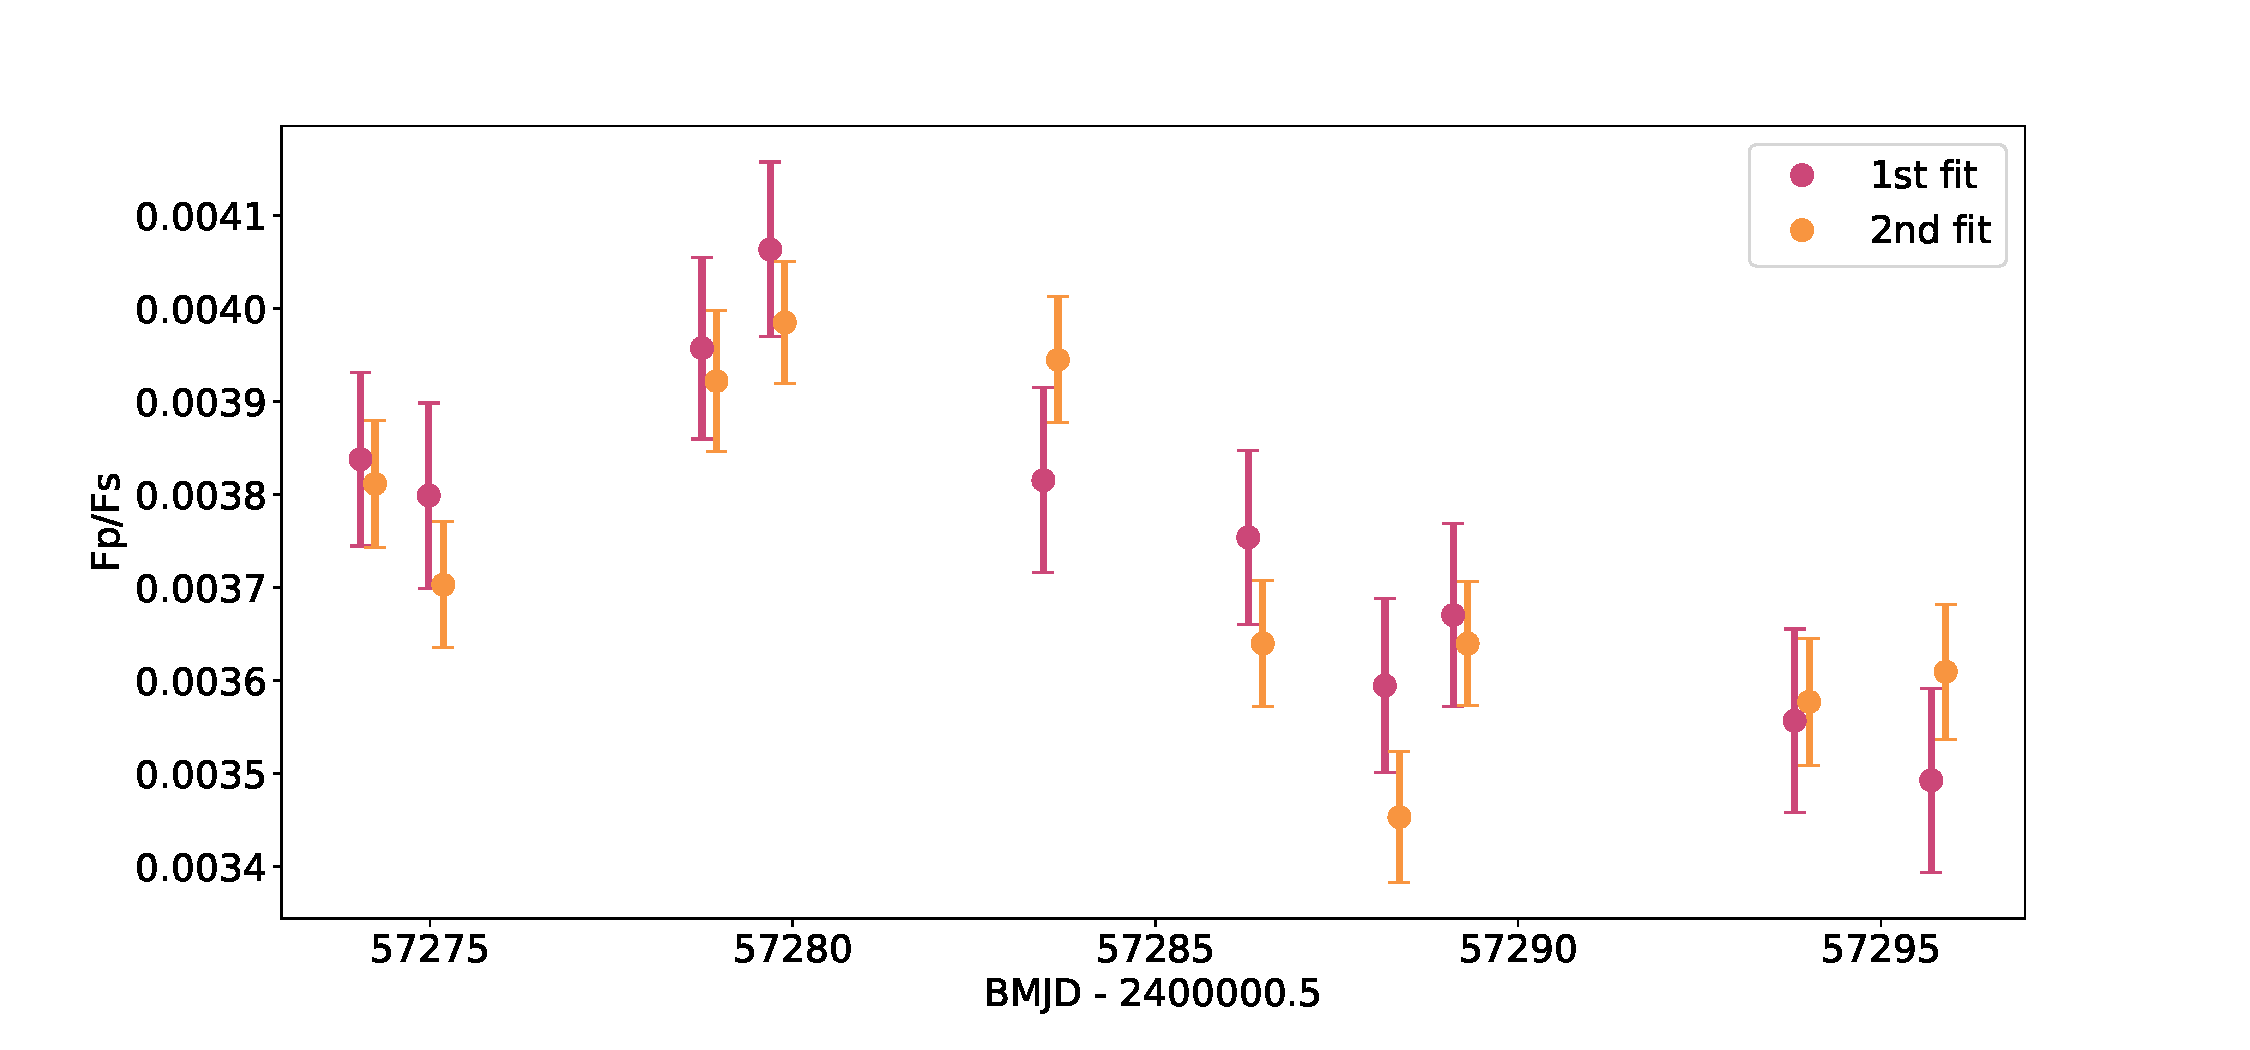
\includegraphics[width=\linewidth]{Wasp18b_EclipseDepths1stv2nd.pdf}
    \caption{Measured eclipse depths of WASP-18b over time in orange, for the ten semi-consecutive eclipses. Pink shows the eclipse depths from the first fit, where all parameters are free. Orange show the eclipse depths from the second fit, where the orbital distance, inclination and \nth{2} order quadratic term are fixed to the weighted mean from the first fit.}
    \label{P3:app:depths}
\end{sidewaysfigure}

\begin{figure}
    \centering
    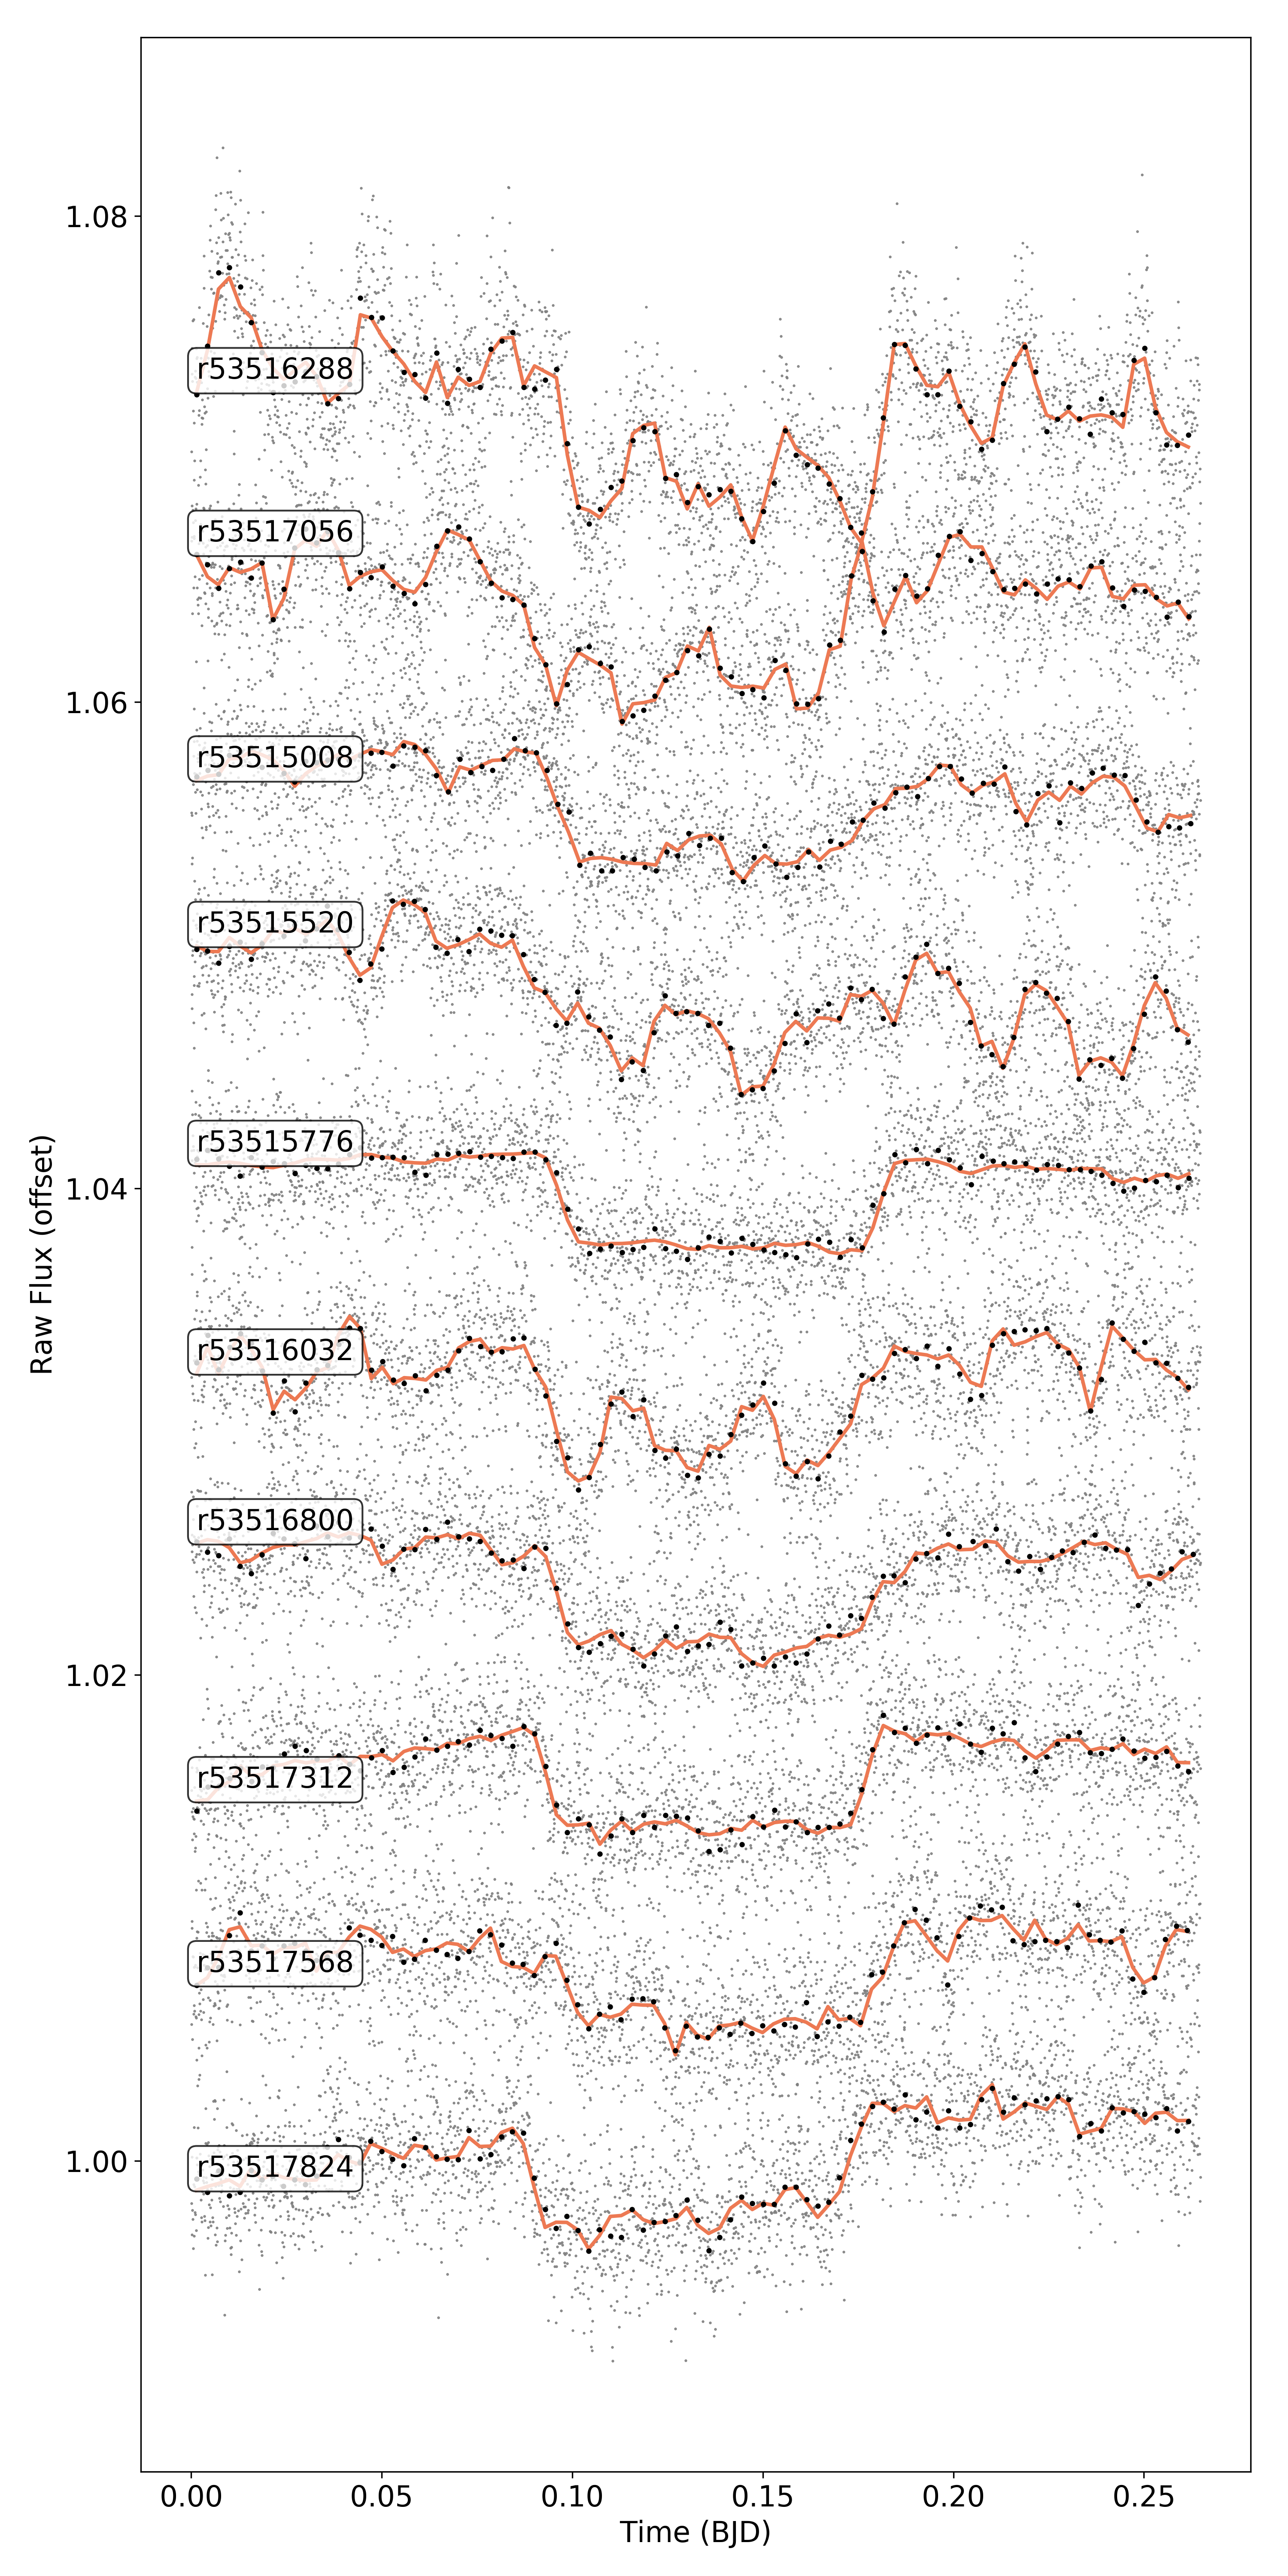
\includegraphics[height=\textheight]{Rawlightcurves_W18b.png}
    \caption{Raw eclipse lightcurves of WASP-18b with best fit systematic and eclipse model in orange.}
    \label{P3:fig:rawlcs}
\end{figure}

\begin{figure}
    \centering
    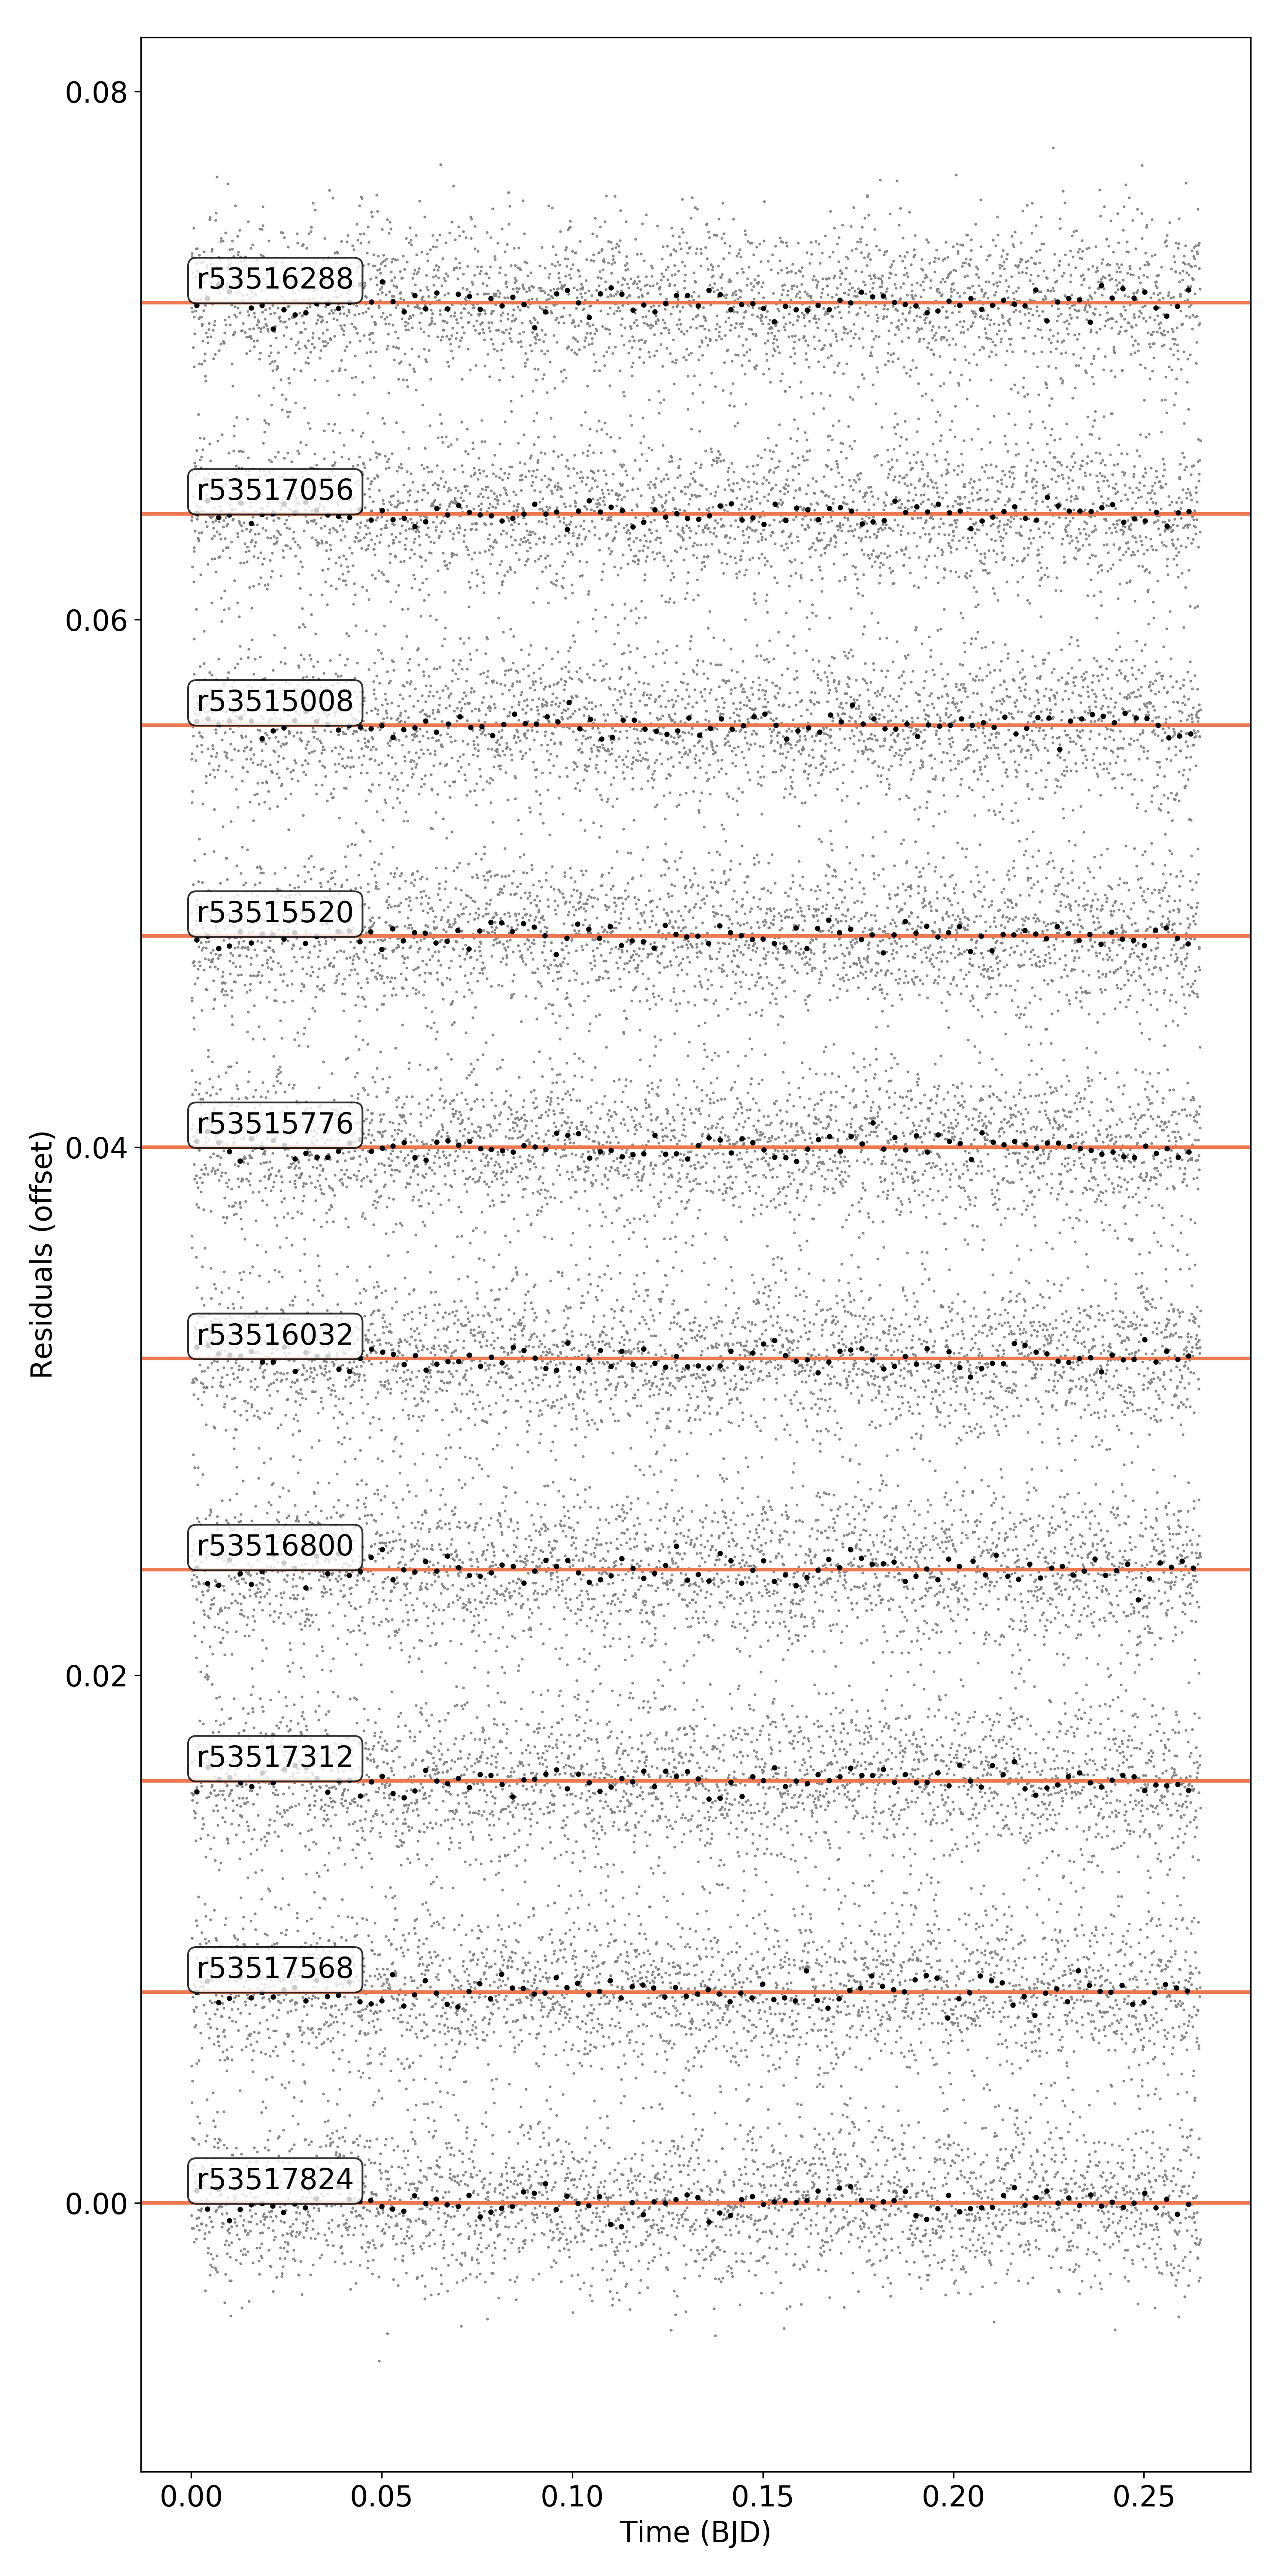
\includegraphics[height=\textheight]{Residuals_W18b.png}
    \caption{Residuals of WASP-18b eclipses with best fit systematic and eclipse model subtracted.}
    \label{P3:fig:residuallcs}
\end{figure}

\end{subappendices}



\begin{appendices}
  %   %% modify slightly header defined in styles/layout.tex
  \titleformat{\chapter}[display]{\LARGE}{\vspace*{-2.3\baselineskip}\raggedleft\textcolor{chcol}{\normalsize
      \chaptertitlename\hspace*{4em}}\\\titlerule\vspace*{0.5pc}{\hrulefill\fontsize{150}{150}\selectfont\textcolor{chcol}{\thechapter}}}{-77pt}{
    \scshape \rmfamily  \linespread{1000}\parbox[t][0pt][c]{0.8\textwidth}}
  \include{content/chapter2/appendix2}
\end{appendices}


%%% ---------------------------------------------------------------------------------------
%%%	BIBLIOGRAPHY
%%%------------------------------------------------------------------------------------------
%%% If you disabled the bibliography entry in the TOC my might use this
%%% command to enable a running head.
% \lhead{{\sffamily \small \slshape Bibliography}}

\setlength{\bibsep}{0.0pt}	%%% controls the reference list items separation

%%% Set bibliography styles:
%%% \bibliographystyle{styles/apj} 		%%% apj style, file apj.bst
%%% \bibliographystyle{styles/aa}        %%% A&A style, file aa.bst
\bibliographystyle{styles/linked-apj} 	%%% Customized apj style that recreates ApJ's colored
					                    %%% hyperlinks to journals [pink] and ADS [blue].
                                        %%% It assumes your bibentries come from ADS, and have

                                        %%% the 'adsurl' keyword.
                                        %%% Do not use this style for print edition!
                                        %%% Do not blindly use this style, it may still have
                                        %%% a few bugs.


%%% Load the bibtex library
%%% You can use multiple libraries, but watch out for double entries!
%%% Also make sure that there are no lingering bibliography or style
%%% definitions in the individual chapters.
\bibliography{content/bibliography/references.bib}


%%%------------------------------------------------------------------------------------------
%%%	BACKMATTER
%%%------------------------------------------------------------------------------------------

%%% The backmatter function turns off chapter numbering
\backmatter
\renewcommand{\chaptermark}[1]{\markboth{\sffamily \small \slshape #1 }{}}  %%% Remove chapter numbering from the headings
%\let\cleardoublepage\clearpage

% !TEX root = ../tex/thesis.tex

% Define a local referenced item command
\newcommand{\coitem}[1]{\item[Chapter~\ref{#1}:] \nameref{#1}}
\newcommand{\coauthors}[1]{\begin{flushleft} {\rm\normalsize #1} \\ \end{flushleft}}
\newcommand{\cojournal}[1]{\begin{flushleft} {\it\normalsize #1} \\ \medskip \end{flushleft}}
\newcommand{\note}[1]{\begin{flushleft} {\footnotesize \normalsize #1} \\ \medskip \end{flushleft}}

% There is no easy way to generate this automatically
\chapter{Contribution from co-authors}
% \vspace*{-1cm}
% \vspace*{1cm}

The position in the author list reflects the importance of the contribution of each co-author. I have omitted Jean-Michel D\'{e}sert from each chapter, as his supervision was present throughout the thesis.

 \bigskip

\begin{description}
% This is where you list the contribution of all your coauthors (see article 15 of the regulations).

  \coitem{ch:intro} %
  %\coauthors{you, your co-authors}
  %\cojournal{Astronomy \& Astrophysics, 20XX, YY, ZZZ}
  \note{The introduction was written entirely by CB.}

  \coitem{transits} %
  \coauthors{Claire Baxter,
            Jean-Michel D\'esert,
            Shang-Min Tsai,
            Kamen O. Todorov,
            Jacob L. Bean,
            Drake Deming,
            Vivien Parmentier,
            Jonathan J. Fortney,
            Michael Line,
            Daniel Thorngren,
            Raymond T. Pierrehumbert,
            Adam Burrows,
            Adam P. Showman}
  \cojournal{Astronomy \& Astrophysics, 648, A127 (2021)}
  \note{CB developed the data reduction pipeline based on previous studies for the reduction of 3.6 and 4.5\um~ Spitzer/IRAC data. Data used in the paper was taken from the Spitzer heritage archive, based on proposals by Jean-Michel D\'esert and Drake Deming. Shang-Min Tsai created the grids of forward models and contributed text to the section describing the models. Daniel Thorngren provided a table of radius anomalies. CB performed all data analysis, comparisons between data and models and wrote the manuscript. All of the co-authors provided feedback to the complete manuscript.}


  \coitem{eclipses} %
  \coauthors{Claire Baxter,
            Jean-Michel D\'esert,
            Vivien Parmentier,
            Michael Line,
            Jonathan J. Fortney,
            Jacob Arcangeli,
            Jacob L. Bean,
            Kamen O. Todorov,
            Megan Mansfield}
  \cojournal{Astronomy \& Astrophysics, 639, A36 (2020)}
  \note{CB augmented the data reduction pipeline for reduction of Spitzer/IRAC eclipses. CB performed the search of the literature and collected all of the eclipse data. Mike Line provided the grid of forward models and contributed text to the section describing the models. Megan Mansfield provided the HST/WFC3 spectra. CB performed all data analysis on the secondary eclipses and the emission models. All of the co-authors provided feedback to the complete manuscript.}

  \coitem{w18b} %
  \coauthors{Claire Baxter \&
            Jean-Michel D\'esert}
  \cojournal{To be submitted to Astronomy \& Astrophysics}
  \note{CB performed the data reduction and analysis of the archival eclipses and wrote the full manuscript. All co-authors provided feedback to the manuscript}

  \coitem{TTVs} %
  \coauthors{Claire Baxter,
            Jean-Michel D\'esert,
            Daniel Fabrycky}
  \cojournal{To be submitted to Astronomy \& Astrophysics}
  \note{CB performed the data reduction of the Spitzer transits. Daniel Fabrycky provided the transit times of the Kepler data, fit TTV models to the Kepler data and provided propagated predictions for the transit times of the multi-planet systems. Daniel Fabrycky also performed photodynamical modelling of the Kepler-16 data from Kepler and provided the relevant text for all of his contributions. CB performed the analysis of the reduced Spitzer transits and made comparisons with TTV predictions. CB wrote the manuscript, with the exceptions of the TTV modelling sections. All co-authors provided feedback to the manuscript.}

\end{description}

%% this is not mandatory
% {
%   \footnotesize

%   \noindent The chapters accepted for publication have been typographically
%   adapted.

%   \noindent
%   The following typos have been corrected:
%   \begin{itemize}
%   \item
%   \end{itemize}
% }


% Reset reference style
\renewcommand\chapterautorefname{chapter}


%%% Local Variables:
%%% mode: latex
%%% TeX-master: "../thesis_renzo"
%%% End:
         %%% mandatory
\chapter[Other publications]{Other publications}

\begin{enumerate}
  \setcounter{enumi}{0}
  \item my other publications
\end{enumerate}

%%% Local Variables:
%%% mode: latex
%%% TeX-master: "../thesis_renzo"
%%% End:
		%%% optional
% !TEX root = ../tex/thesis.tex

% This makes Figure A instead of Figure 1
\renewcommand{\thefigure}{\Alph{figure}}

% This resets the figure counter
\setcounter{figure}{0}

% reset the footnote counter
\setcounter{footnote}{0}

% Set language to Dutch for correct word-breaks.
% It also changes the Figure into Figuur, etc.
\selectlanguage{dutch}
\renewcommand\chapterautorefname{hoofdstuk}%
\cleardoublepage

\chapter{Nederlandse Samenvatting}

\lipsum[6]
 

% Reset language
\selectlanguage{english}
\renewcommand\chapterautorefname{chapter}%


%%% Local Variables:
%%% mode: latex
%%% TeX-master: "../thesis_renzo"
%%% End:
 	    %%% mandatory
%%% % !TEX root = ../tex/thesis.tex

% This makes Figure A instead of Figure 1
\renewcommand{\thefigure}{\Alph{figure}}

% This resets the figure counter
\setcounter{figure}{0}

% reset the footnote counter
\setcounter{footnote}{0}

% Set language to Dutch for correct word-breaks.
% It also changes the Figure into Figuur, etc.
%\renewcommand\chapterautorefname{hoofdstuk}%
\cleardoublepage

\chapter{Summary}

The Spitzer Space Telescope was decommissioned in January 2020, leaving behind a legacy of rich atmospheric studies of individual exoplanets. This thesis summarizes the huge efforts of Spitzer in the field of exoplanet science over the last 15 years. Using several hundreds of hours of near-infrared Spitzer/IRAC observations in emission and transmission, we measured and characterized the atmospheres of more than 100 exoplanets in total. We gained a deep understanding of the complex instrumental systematics involved in analyzing such data and we pinned down the important physical processes required in atmospheric models.

In Chapter \ref{transits} we presents our Spitzer/IRAC data reduction pipeline. This pipeline implements pixel level decorrelation for correcting the strong systematics arising from the intrapixel sensitivity of the IRAC detectors. We used this procedure to analyze 70 photometric lightcurves of 33 transiting planets uniformly. We then augmented this sample with 16 previously published exoplanets, resulting in a total of 49 exoplanets with transmission measurements at 3.6 and 4.5\um.

We compare the survey of exoplanet transit depths to a grid of 1-D radiative convective equilibrium forward models. Our initial grid of models stands on two common assumptions when modelling exoplanet atmospheres. First, is that the atmosphere is in chemical equilibrium. This means that the abundance of different molecular species can be determined from the temperature, pressure, and global chemical composition of the atmosphere. Second, it is commonly assumed that the elemental chemical composition of a typical atmosphere is equivalent to that of the Sun (solar composition). Under these assumptions, models can predict the relative abundance of elemental and molecular species as a function of planet temperature and pressure probed by transmission spectroscopy. In particular, a transition from methane to carbon monoxide is expected at around 1000 K as we sample from the coolest close-in giant exoplanets to the hottest hot-Jupiters. We demonstrated this transition with our grid of equilibrium chemistry solar composition forward atmospheric models. However, when comparing our models to our observations we found that the models overestimate methane levels for the coolest planets. With 13 planets less than 1000K, we obtained a strong statistical confirmation ($7.5~\sigma$) of the lack of methane in the atmospheres of gas giant exoplanets for the first time ever.

Building on this, we expanded our grid of models from equilibrium chemistry and solar composition to include disequilibrium chemistry as characterized by vertical mixing (via an eddy diffusion coefficient, $K_{zz} = 0$ - $10^{12}$~\cmcms) and with two different chemical compositions (1x and 30x solar). By comparing these models to the observations we were able to show that the lack of methane in the cool planets can be partially explained with models of higher metallicity (30x solar) and rule out the models with 1x solar composition with >$3~\sigma$ confidence. Previous studies have suggested that there is a mass-metallicity relation in the bulk composition of transiting gas giant planets, whereby the less massive planets tend to be more metal rich. Our finding supports the extrapolation of this trend from bulk metallicities to atmospheric metallicities.

Additionally, we found that these coolest planets (<1000K) favor the models with low amounts of vertical mixing ($K_{zz} = 10^8$~\cmcms). So not only do these cool, less massive close-in gas giant planets have statistically more metal-rich atmospheres than their hotter counterparts, they also exhibit less vigorous vertical mixing. On the other hand, we found that the hottest planets (>1000K) are best explained by 1x solar metallicity and high vertical mixing models ($K_{zz}= 10^{12}$~\cmcms). Higher levels of vertical mixing in hotter atmospheres has been predicted theoretically and observed in the atmospheres of brown dwarfs. Our result supports both of these studies.

In our survey of transiting planets, we did not find any obvious trends in the transmission metric with increasing temperature for the ultra-hot planets, but we only have a few ultra-hot Jupiters in our sample. However, in Chapter \ref{eclipses}, we expanded our exploration to the dayside emission of exoplanets. We used a survey of 78 planets with secondary eclipses to explore how the abundance of \ce{CH4} and CO manifests in the dayside. This survey contained twice as many hot planets compared with the transmission survey, and only a few of which fall within the expected methane-dominated temperature range. Furthermore, emission photometry probes deeper in the atmosphere (~1-10 bar pressure levels) than transmission photometry (~1mbar pressure level), reaching levels of higher temperatures and likely low methane abundance.

We examined this sample of planets by calculating the 3.6 and 4.5~\um~ brightness temperatures of the planetary dayside. We also defined a metric, called deviation from the blackbody, which measures the emission or absorption of the 4.5~\um relative to the 3.6~\um~ bandpass. The 4.5~\um~ probes the CO feature and the 3.6~\um~ probes close to the continuum due to the lack of methane in the hotter planets. Therefore, this metric allows us to probe the temperature pressure profile by measuring the strength of the relative CO emission or absorption. We found a transition in the deviation from the blackbody between the hot and the ultra-hot Jupiters at around 1700K, where the hotter planets appeared to have a stronger CO feature in emission. We explored what the origins of this might be by comparing the result to a new grid of self-consistent 1D radiative and convective models varying metallicity, carbon to oxygen ratio (C/O), surface gravity, and stellar effective temperature, making sure to incorporate the relevant physics for temperature inversions to form. The data is in remarkable agreement with these models. We propose that the transition between hot and ultra-hot Jupiters is statistical evidence of temperature inversions in the hottest planets, in addition to the expected Planck function shift.

Chapter \ref{eclipses} highlights the crucial importance of careful calculation of brightness temperatures and effective temperature. We found that either a failure to integrate over the Spitzer bandpass or approximating the star with a blackbody instead of a PHOENIX model when calculating the brightness temperatures can induce a bias in the results. This bias resulted in increasing the measured effective temperature of the planet compared to the equilibrium temperature prediction, and the bias was stronger for the planets around hotter stars. These disproportionately hotter effective temperatures in hotter exoplanets can be misinterpreted as a lower efficiency of redistribution in the hottest planets as is seen in previous studies. Another source of bias arises from the fact that the effective temperature is typically calculated by fitting a blackbody to the spectral energy distribution of the planet. However, there are just two photometric points, one of which has a strong CO emission feature (4.5~\um~) for the cases of ultra-hot Jupiters. In such a situation, calculating the effective temperature as a weighted mean of the two Spitzer brightness temperatures also biased the effective temperature results towards hotter temperatures. After correcting for all of these effects, we did not find a statistically significant trend in the effective temperature with equilibrium temperature. This finding does not support previous claims of lower redistribution efficiency with hotter planets. However, there remained a large scatter in the brightness temperatures of hotter planets compared to cooler planets, which suggested a range of different redistribution efficiencies for the hottest planets.

In Chapter \ref{w18b} we analyzed 10 archival secondary eclipses of the ultra-hot Jupiter WASP-18b and found periodic variability in the 4.5~\um~brightness of the planet in time. Using a sinusoidal model, we derived a variability period of 23.12 $\pm$ 1.66 days and a peak-to-trough amplitude of 456 $\pm$ 71~ppm, corresponding to $\sim$12\% variability. We discussed possible physical processes that could result in such variability: magnetic field coupling, variable wind speeds, clouds, changes in chemical composition, and we ruled out the hypothesis that this was due to stellar variability. Finally, we explored whether this could be detected with the current state-of-the-art instruments (HST, TESS) and found that these do not have the required precision and that we need to look towards future missions for follow-up of these variability measurements.

In Chapter \ref{TTVs} we analyzed 48 transits of the lowest SNR planets that were chosen for the science exploration program. We measured the transit times of six planets from three multi-planet systems (Kepler-9, Kepler-18 and Kepler-32) and compared these transit times to predictions made from Kepler observations. We found that the uncertainties were quite large on the Spitzer transits and so the results were consistent with predictions but not accurate enough to further constrain the models. Additionally, we analyzed two transits of the circumbinary planet, Kepler-16b.

#### INSERT SENTENCES ABOUT KEPLER 16B ####

The work presented in this thesis has the potential to serve as the benchmark for infrared studies in the future of exoplanet science, particularly with the upcoming James Webb Space Telescope. The trends observed and the effects described in the studies reported (vertical mixing, temperature inversions, clouds, variability, and complex dynamics) will be even more apparent with the increased precision, and important to include in future modelling efforts. Our research contributes to the understanding of planetary atmospheres in a broad context, thereby illuminating the issues of planet formation, evolution, and, ultimately, habitability.  

% Reset language
\selectlanguage{english}
\renewcommand\chapterautorefname{chapter}%


%%% Local Variables:
%%% mode: latex
%%% TeX-master: "../thesis_renzo"
%%% End:
 		%%% mandatory -- not if it is in the intro!
% !TEX root = ../tex/thesis.tex

\setcounter{footnote}{0}


\chapter{Acknowledgements}


\vspace{10mm}

It's no secret that finishing the PhD was a difficult feat for me. I don't think I would have managed it without all the help and support I have received from colleagues, friends and family over the last four and a half years. Everybody I have interacted with has, in some way or form, shaped me and my journey through the PhD and I owe many of these people a special thank you.

First, I want to thank my supervisor. You provided me with the opportunity to move to Amsterdam and do a PhD in the first place. I learned a lot from working with you. Scientifically, professionally and personally. I will take this wisdom to my future endeavours even though I have left academia. It was also amazing to see you grow the group of exoplaneteers at API over the last few years. You have built a group of amazing scientists and I look forward to seeing the great science that each of them produces in the future.

Speaking of the group, I have discovered and learned so much from our meetings, group meetings, and conversations over the years. Thank you for being such an awesome team.

Thank you as well to all of my collaborators for reading my papers, providing insightful feedback and creating models for me. I learned a lot from my discussions with you and your contributions always made my papers better. An additional thanks to all of the conference/workshop/meeting/summer school organisers throughout the years. My interactions (social and professional) at all of these events greatly enhanced my PhD experience, I am lucky to have met and travelled with so many great people.

I would also like to express my gratitude to the API for being such a warm and accepting environment for me to be a researcher. From the first time I set foot in the Institute during my interview days, I felt immediately welcomed and included in the community. So a huge thanks to all of the staff, PhDs, postdocs, and students who play an important role in making the institute a special and unique place to do a PhD. I feel honoured to have been a part of such a great and forward-thinking community.

Before embarking on a PhD, I worked on several projects and was fortunate to have had a string of great scientists as supervisors. This was especially motivating as all of you happened to be women. You showed me that astrophysics is a place for everyone and I am deeply grateful to each of you. You gave me the support, guidance and encouragement I needed and ultimately inspired me to pursue a PhD. I couldn't believe my luck when one of you was already working at API when I started!

Speaking of strong females, I want to say a special thanks to the pillars (secretariat) of the API, for holding the place together, especially through all the chaos over the last few years. The Institute would not be the same without you, I think I speak for everyone when I say that you are the glue that brings everyone together and make API such a brilliant community to be a part of. You have always surpassed your official duties, and were always a friendly shoulder to cry on with a seemingly endless supply of sweeties. An additional thanks to the PhD evaluation committee, our director and my promotor for doing your best to take care of us and for making the PhD journey as smooth as possible.

Continuing with thanking the APIs, thanks to my two little hobbits, for all of the fun, beers, movie nights, travel adventures and for being great and supportive friends through all of the ups and downs of the PhD. Thanks to my API buddy for taking me under her wing at the beginning, for giving me the courage to be brave and for trying to teach me how to dance. Thanks to the API noobs and bake-off partners in crime for all of the delicious cake, dinners, risotto lessons and python help. Thanks to the API-in law who designed my wonderful thesis cover and to the one who always had Tea. Thanks to the avengers and quarantine bikers for the adventures, bike rides and for all of the fun socialising keeping me sane. Thanks to all of my office mates over the last 4 years for making the days at the office gezellig and productive. I will miss the random chats and the fancy coffee breaks. A special thanks to my two paranymphs: my little PhD brother and my fellow Brit abroad/wine buddy. I look forward to seeing both of your PhD theses soon.

A further thanks to all of the API athletes for all of the sporting adventures and fun over the years. I never thought a bunch of astronomers would run 160km through Germany in the middle of the night, but we did it! On the other hand, I never had any doubts that we would be able to party after running 160km. Thanks to my swimming partner, for the therapy and for pushing me to pick up biking and running as well. Thanks to my new swimming partner, for letting me convince him to join the triathlon club. And thanks to all the swimmers, gymmers and triathletes who have helped keep me fit and sane through the stressful moments.

Thanks to the Montelbaaners, for the Michelin star meals, the live music concerts, the pool parties, and the set of great memories. You guys were so welcoming, you introduced me to so many great people and I really felt like I had a second family in you all. Coming home to you guys turned the hard days into beautiful days. Additionally, a special thank you to all my homies in the West for the unconditional support, the extravagant brunches, the drunken evenings, the board games, the face squeezes, the Kubb in the park, and the walks when there was nothing else we could do. I look forward to more great adventures with you all.

Thanks to my physics pals and ex-housemates from Edinburgh, I can't wait to be reunited with you all again and to go on more ski trips in the future. A special thanks to the one who will always be up for spending a weekend in our pyjamas baking cookies no matter what extravagant location we happen to be meeting in. You guys made studying physics fun, which inspired me to pursue it further. I am extremely grateful for all the support and good times that we had over the years.

From school classmates to teenage party buddies, to making a WhatsApp chat solely dedicated to pictures of cats for when we're sad, you know who you are. Your friendship means the world to me. I am extremely grateful for everything that you have done for me and all of the good times we have had throughout the years, there are too many to list. A special thanks to your direct contribution to this thesis by kindly giving me feedback on my writing, I know it must have taken you a lot of time to read and understand my rambles. You are an amazing friend and I am honoured to be able to call you that, thank you for everything.

To the one to whom I almost got engaged. I am eternally grateful to you. You are always there when I need you and you have provided me with so much support and help ever since I knew you, especially with the writing! We have shared so many hilarious moments and I am extremely thankful for your friendship. Less than infinity.

To the guy who fixed my internet. Thank you for all of the support you gave me, for teaching me to trust myself, helping me grow, become a stronger person and dampening the tidal waves of the PhD with your calm and gentle approach to life.

The final words go to my wonderful parents and brother. I probably wouldn't even have chosen to study physics if I didn't look up to my big brother the way that I did. You always encouraged me to ask questions, think critically and carefully and inspired me to aim high. I know we don't speak every day, but I take a lot of comfort in knowing that you are always there for me if I need it. You are an amazing big brother and I wouldn't be the person that I am without you. As for our parents, I can very literally say that I wouldn't even be here without both of you. You have always supported me in every way possible no matter what happens. You let me follow my own path in life and have always been there without fail. Dad, you have taught me the value of being loyal, strong, standing up for myself yet always looking out for others. Mum, you are so kind, generous and patient with everyone in your life. I can talk to you about anything and everything, and you are always there to listen. You are all my rocks, none of this would have been possible without you, and I still have so much to learn from each of you.


\raggedleft
Claire

%%% Local Variables:
%%% mode: latex
%%% TeX-master: "../thesis_renzo"
%%% End:



%% For Ylva: first person I met in AMS
%% For Manos: SNe understanding at 3am in Chicheley Hall
%%
  %%% optional (but not really!)
% !TEX root =  thesis.tex

\cleardoublepage
\thispagestyle{empty}
{\raggedright
  \small
  \noindent Ph.D.~thesis, Anton Pannekoek Institute, Universiteit van Amsterdam\\
  \noindent Claire Julie Baxter, 2021\\
    \noindent \textit{Contact: cbaxter93@icloud.com} \\[3ex]

  \noindent ISBN: \todo{N} \\[3ex]

  \noindent Cover design by Tamzyn Revolta.\\
  %\noindent Credits:



  %\noindent The source files for this thesis are available
}



\cleardoublepage
\thispagestyle{empty}
\null\vfill\null

\hfill\parbox{125mm}{
\raggedleft\emph{\large Above all, don’t fear difficult moments. The best comes from them.}\\[5pt]
Rita Levi-Montalcini
}
\vfill
\clearpage
\thispagestyle{empty}
\newpage
\phantom{let's kill those trees}


\pagestyle{fancy}

%%% Local Variables:
%%% mode: latex
%%% TeX-master: "../thesis_renzo"
%%% End:
        %%% optional
\end{document}

%%% Local Variables:
%%% mode: latex
%%% TeX-master: t
%%% End:
